\documentclass[12pt, italian]{toptesi}
\usepackage[T1]{fontenc}
\usepackage[utf8]{inputenc}
\usepackage{lmodern}
\usepackage[italian]{babel}
\usepackage{pdfpages}
\usepackage{caption}
\captionsetup{tableposition=top,figureposition=bottom,font=small}
\usepackage[autostyle,italian=guillemets]{csquotes}
\usepackage[backend=biber]{biblatex}
\usepackage{booktabs}
\usepackage{siunitx}
\sisetup{output-decimal-marker={,}}
\usepackage{tabularx}
\addbibresource{bibliografia_tesi.bib}

\unless\ifTOPfront% esegue solo se si è specificata l'opzione "noTOPfront"
   \usepackage{frontespizio}
\fi

\usepackage{hyperref}

\hypersetup{%
    pdfpagemode={UseOutlines},
    bookmarksopen,
    pdfstartview={FitH},
    colorlinks,
    linkcolor={black},
    citecolor={red},
    urlcolor={black}
  }
  
\begin{document}

\frontespizio

\paginavuota
\begin{dedica}
       A mia madre
\end{dedica}

\ringraziamenti

Vorrei innanzitutto ringraziare l'Ing.~Loiacono per il preziosissimo aiuto fornitomi durante la tesi, per essere sempre stato disponibile ad aiutarmi e per avermi fatto prendere la decisione giusta per la tesi. 
Lo ringrazio anche per avermi fornito i due computer su cui ho svolto la maggior parte degli esperimenti, senza i quali non sarei riuscito a finire questa tesi.

Vorrei anche ringraziare Piero Uboldi e la redazione del Notiziario per l'aiuto dato e per avermi concesso l'uso di computer per gli esperimenti.

Un grosso grazie va a tutte le persone che ho conosciuto in questi 5 anni di università, in particolar modo i miei compagni di corso, senza i quali questi 5 anni non sarebbero stati gli stessi.

Ringrazio tutte le persone che ho conosciuto in Erasmus che mi hanno fatto passare uno dei periodi più belli della mia vita, in particolare Marco, Riccardo, Dalila, Nico, Vale, Jenny, Maxime, Juliette e Massi.
Ringrazio tutti i miei zii, i miei cugini Luca, Nicola, Lorenzo, Stefano, Sarah, Matteo, Giancarlo, Giada e Jacopo; tutti i miei amici milanesi, Marco, Ivan e Davide; i miei amici lecchesi Luca, Greg, Giulia, Francesca, Daniele, Carlo, Davide, Paolo, Valentina, ecc.; gli amici di Onore Andrea, Serena, Giulio, Robi, Elisa, Annalisa, Claudia, Simo, Lorenzo, Michele ecc.

Ultimo ringraziamento ma sicuramente non per importanza a mia madre, a cui non potrò mai smettere di dire grazie per tutto quanto,  per avermi cresciuto, per avermi aiutato in tutta la mia carriera scolastica e universitaria, e per avermi sempre sostenuto nelle mie decisioni, Grazie.

\indici

\listoffigures
\listoftables

\abstract

La creazione automatica di contenuti è un processo che sta assumendo un'importanza sempre maggiore nello sviluppo dei videogiochi moderni.
Infatti le tecniche di generazione procedurale possono diminuire i tempi di sviluppo ed aiutare gli sviluppatori a creare contenuti che rispettino gli alti standard qualitativi richiesti nelle moderne produzioni videoludiche.
Questo lavoro vuole fornire uno strumento capace di creare automaticamente armi per gli sparatutto in prima persona.
La generazione avviene rispettando alcuni requisiti fondamentali che permettono di ottenere armi interessanti, bilanciate e funzionali.
Utilizzando un famoso titolo commerciale come test delle funzionalità delle armi, \emph{Unreal Tournament III}, utilizziamo un algoritmo genetico per generare automaticamente i parametri delle armi.
Abbiamo condotto tre diversi esperimenti con diverse finalità: nel primo esploriamo lo spazio di design delle armi con lo scopo di generare armi diverse tra loro e che siano equilibrate e funzionali;
nel secondo calibriamo un'arma data con lo scopo di bilanciarla; nel terzo esploriamo dello spazio di design con alcuni obiettivi aggiuntivi, che formalizzano alcuni requisiti di gameplay.
Per ogni esperimento analizziamo i risultati ottenuti e mostriamo le armi generate più interessanti.

\selectlanguage{english}

\abstract
Nowadays the procedural generation of content is getting an incremental attention in the video game panorama.
It can help designers to create new content and at the same time it can reduce development cost and time.
This work wants to provide a tool that can help game designers to create weapons for first person shooter games.
By using well known techniques of procedural content generation, e.~g.~genetic algorithms, this tool
can create offline couple of weapons, and provides a set of control parameters to direct the creation.
To test the weapons generated we use a famous commercial game: \emph{Unreal Tournament III}.
We have conducted three main experiments.
In the first one we explore the space of weapons in order to obtain couple of balanced and usable weapons.
On the second one, we balance a given weapon designed by a game designer.
In the third one we have added some external parameters to direct the weapon generation, which address some important gameplay feature.
We describe the results obtained in each experiment and then we analyze some interested weapon picked from the generated ones. 

\selectlanguage{italian}


\mainmatter

\chapter{Introduzione}

Oggigiorno la produzione dei videogiochi è un processo sempre più complesso, che richiede lunghi periodi di sviluppo e risorse per costruire l'alto numero di contenuti che necessitano le produzioni moderne.
Infatti la ricchezza di contenuti è fondamentale per il successo commerciale di un videogioco, e gli alti standard qualitativi richiesti dagli utenti necessitano di lunghe fasi di test per verificare la qualità dei contenuti e il design delle meccaniche di gioco.
Negli sparatutto in prima persona uno dei componenti fondamentali per il gameplay sono le armi. Queste richiedono un attento design che permetta di sviluppare varie strategie che rendano complesso ed appagante l'esperienza di gioco: le armi devono essere varie, divertenti da usare, equilibrate, ecc.
La fase di design delle armi richiede un conoscenza approfondita delle meccaniche di gioco e numerosi test con persone fisiche che possono allungare i tempi di sviluppo e richiedere investimenti aggiuntivi.
Quindi automatizzare il processo di creazione delle armi potrebbe giovare sia dal punto di vista economico sia dal punto di vista dei tempi di sviluppo.

Per questo motivo abbiamo sviluppato uno strumento per la generazione automatica di armi.
Nel nostro lavoro ci concentriamo nella generazione automatica di armi per sparatutto in prima persona competitivi, armi che devono rispettare alcuni requisiti di gameplay.
Abbiamo studiato l'utilizzo di tecniche di apprendimento automatico per creare uno strumento che semplifichi ai game designer la creazione di armi.
In particolare ci siamo avvalsi dell'utilizzo di algoritmi genetici, che permettono di creare automaticamente delle armi attraverso la modifica dei parametri funzionali dell'arma.
Attraverso l'uso del videogioco \emph{Unreal Tournament III} e della sua intelligenza artificiale, simuliamo una partita tra due giocatori, che ci permette di valutare le prestazioni delle armi generate.
Lo studio si è focalizzato su tre scenari: 
\begin{enumerate}
\item Esplorazione dello spazio di design delle armi con lo scopo di generare armi diverse tra loro e che siano equilibrate e funzionali;
\item Calibrazione automatica di un'arma obiettivo creata \emph{ad-hoc} da un game designer;
\item Esplorazione dello spazio di design con alcuni obiettivi secondari, che vanno a indirizzare la generazione verso alcuni requisiti di gameplay.
\end{enumerate}

Nella letteratura possiamo trovare lavori dedicati al bilanciamento dei FPS ma diretti alla creazione di mappe; mentre per quanto riguarda le armi, la ricerca accademica si è concentrata nella generazione procedurale con l'obiettivo finale di creare armi innovative, senza però dedicarsi al bilanciamento o altri requisiti di game design, se non con soluzioni ad-hoc.
Quindi il nostro lavoro vuole essere un \emph{trait d'union} tra questi due lavori, cioè il bilanciamento negli sparatutto e la generazione automatica di armi.

Questa tesi è strutturata come segue: 

\bigskip

Nel \textbf{Capitolo 2} descriviamo la \emph{Generazione Procedurale di Contenuti} (PCG), in particolare facciamo un piccolo \emph{excursus} storico della PCG, e successivamente ne descriviamo la tassonomia. Infine portiamo alcuni esempi di generazione procedurale con algoritmi di ricerca, in particolare la generazione di mappe e di armi.

\bigskip

Nel \textbf{Capitolo 3} andiamo a descrivere gli obiettivi di questo lavoro e l'ambiente sviluppato per condurre gli esperimenti. Nella prima parte descriviamo i nostri obiettivi e il gioco usato per le simulazioni: Unreal Tournament III.
Nella seconda parte andiamo a descrivere l'ambiente simulativo in cui si svolgono gli esperimenti e le modifiche apportate al gioco UT3 per svolgere le simulazioni.

\bigskip

Nel \textbf{Capitolo 4} mostra i risultati del primo esperimento, cioè la generazione di armi equilibrate senza nessun vincolo aggiuntivo; successivamente andiamo ad analizzarne i risultati ed alcuni esempi di armi generate. Infine mostriamo l'errore ottenuto rivalutando i risultati finali con un numero limite di uccisioni per partita più ampio.

\bigskip

Nel \textbf{Capitolo 5} mostra i risultati ottenuti del secondo esperimento, dove il nostro obiettivo è il bilanciamento di un'arma obiettivo, da bilanciare contro un'arma fissa. Per questo abbiamo selezionato due armi già implementate in UT3, cioè abbiamo provato a bilanciare l'arma denominata \emph{Flak} contro l'arma chiamata \emph{Rocket Launcher}. Infine andiamo a validare i risultati ottenuti con delle simulazioni più precise.

\bigskip

Nel \textbf{Capitolo 6} mostra i risultati ottenuti con il terzo esperimento, dove l'obiettivo è generare armi bilanciate con dei vincoli specifici per arma.
In particolare abbiamo scelto tre obiettivi da massimizzare: la distanza media dei colpi, il tempo impiegato per colpire un avversario (\emph{Hit time}) e le sequenze di uccisioni (\emph{Kill Streak}).
Successivamente andiamo a valutare l'errore dei risultati mediante delle simulazioni più precise.

\bigskip

Nel \textbf{Capitolo 7} riportiamo le conclusioni di questo lavoro e i possibili sviluppi futuri.

\chapter{Generazione procedurale di contenuti}

In questo capitolo introdurremo la generazione procedurale di contenuti (\emph{Procedural Content Generation, PCG}).
Successivamente andiamo a descrivere la tassonomia di questo campo di ricerca.
Infine vedremo degli esempi applicativi di PCG nel genere videoludico degli \emph{First Person Shooter}, in particolare la generazione automatica di mappe e di armi.

\section{Procedural Content Generation}

La generazione procedurale di contenuti consiste nel lasciare il computer l'onere di creare automaticamente i contenuti di un videogioco, come per esempio circuiti, mappe, pianeti, mostri, animazioni ecc.
Le PCG nasce per risolvere problematiche dovute a limitazioni hardware che impedivano di poter salvare in memoria grandi quantità di contenuti.
Quindi si generava attraverso il codice i contenuti necessari al videogioco.
La prima apparizione della PCG la troviamo nel gioco \emph{Beneath Apple Manor} \footnote{\url{http://en.wikipedia.org/wiki/Beneath_Apple_Manor}} (1978),
un gioco bidimensionale dove l'obiettivo è trovare una mela dorata alla fine di un labirinto.
Qui è già possibile trovare una generazione automatica dei livelli e il posizionamento dei nemici e dei tesori è automaticamente generato all'inizio del gioco.
Un altro esempio famoso è \emph{Elite}, un gioco di simulazione spaziale, dove troviamo un avanzato sistema di commercio. Questo viene gestito da un algoritmo di generazione automatica dei prezzi e della posizione dei materiali grezzi all'interno dell'universo del gioco, e inoltre anche il nome e la descrizione dei pianeti sono creati automaticamente attraverso la PCG.
\begin{figure}
\centering
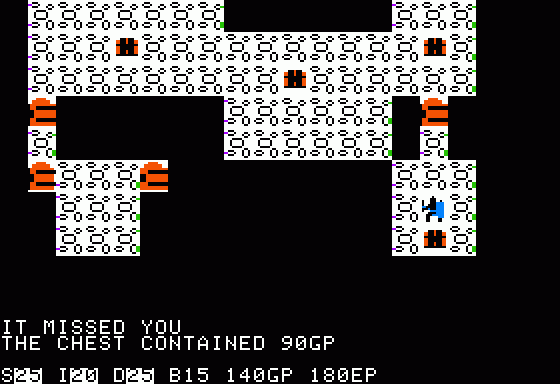
\includegraphics[width=0.5\textwidth]{beneath_apple_manor}
\caption{Beaneath Apple Manor}
\label{fig:beneath_apple_manor}
\end{figure}
\begin{figure}
\centering
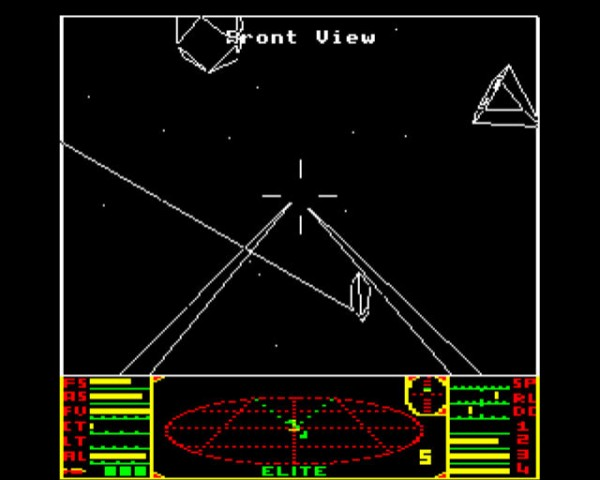
\includegraphics[width=0.5\textwidth]{elite}
\caption{Elite}
\label{fig:elite}
\end{figure}
Oggi non ci sono più le stesse limitazioni hardware dei primi giochi, ma nonostante questo abbiamo una crescita esponenziale d'uso di tecniche di PCG.
Infatti la PCG oggi è utilizzata per aumentare l'efficienza degli studi di sviluppo, per esempio attraverso l'uso di strumenti commerciali, o per essere inserita come elemento portante delle meccaniche di gioco, cioè basando alcuni elementi necessari alla fruizione del gioco proprio sulla generazione procedurale.
Tra gli strumenti commerciali più famosi citiamo \emph{SpeedTree}, il quale è capace di creare automaticamente alberi e foreste ed è utilizzato da molti giochi commerciali, tra cui \emph{Skyrim}, un gioco di ruolo in prima persona sviluppato da Beteshda Software \footnote{\url{http://en.wikipedia.org/wiki/The_Elder_Scrolls_V:_Skyrim}}; \emph{CityEngine} \footnote{\url{http://en.wikipedia.org/wiki/CityEngine}}, che può creare intere città ed edifici.
Per quanto riguarda invece i giochi per cui sono stati sviluppati soluzioni \emph{ad-hoc} direttamente dallo studio di sviluppo troviamo: \emph{Spore}, gioco manageriale/strategico dove le animazioni delle specie inventate nel gioco sono create proceduralmente; \emph{No Man's Sky} \footnote{\url{http://en.wikipedia.org/wiki/No_Man's_Sky}}, un gioco di avventura nello spazio, dove la PCG è usata per creare l'intero gioco, dai pianeti fino alle specie che è possibile trovare su di essi.
Infine relativo all'argomento di questa tesi, citiamo anche \emph{Borderlands} \footnote{\url{http://en.wikipedia.org/wiki/Borderlands_(video_game)}},
sparatutto in prima persona, dove ogni arma presente nel gioco è una combinazione di vari elementi diversi, con i quali il gioco è capace di creare una quantità notevole di armi.

\begin{figure}

\centering
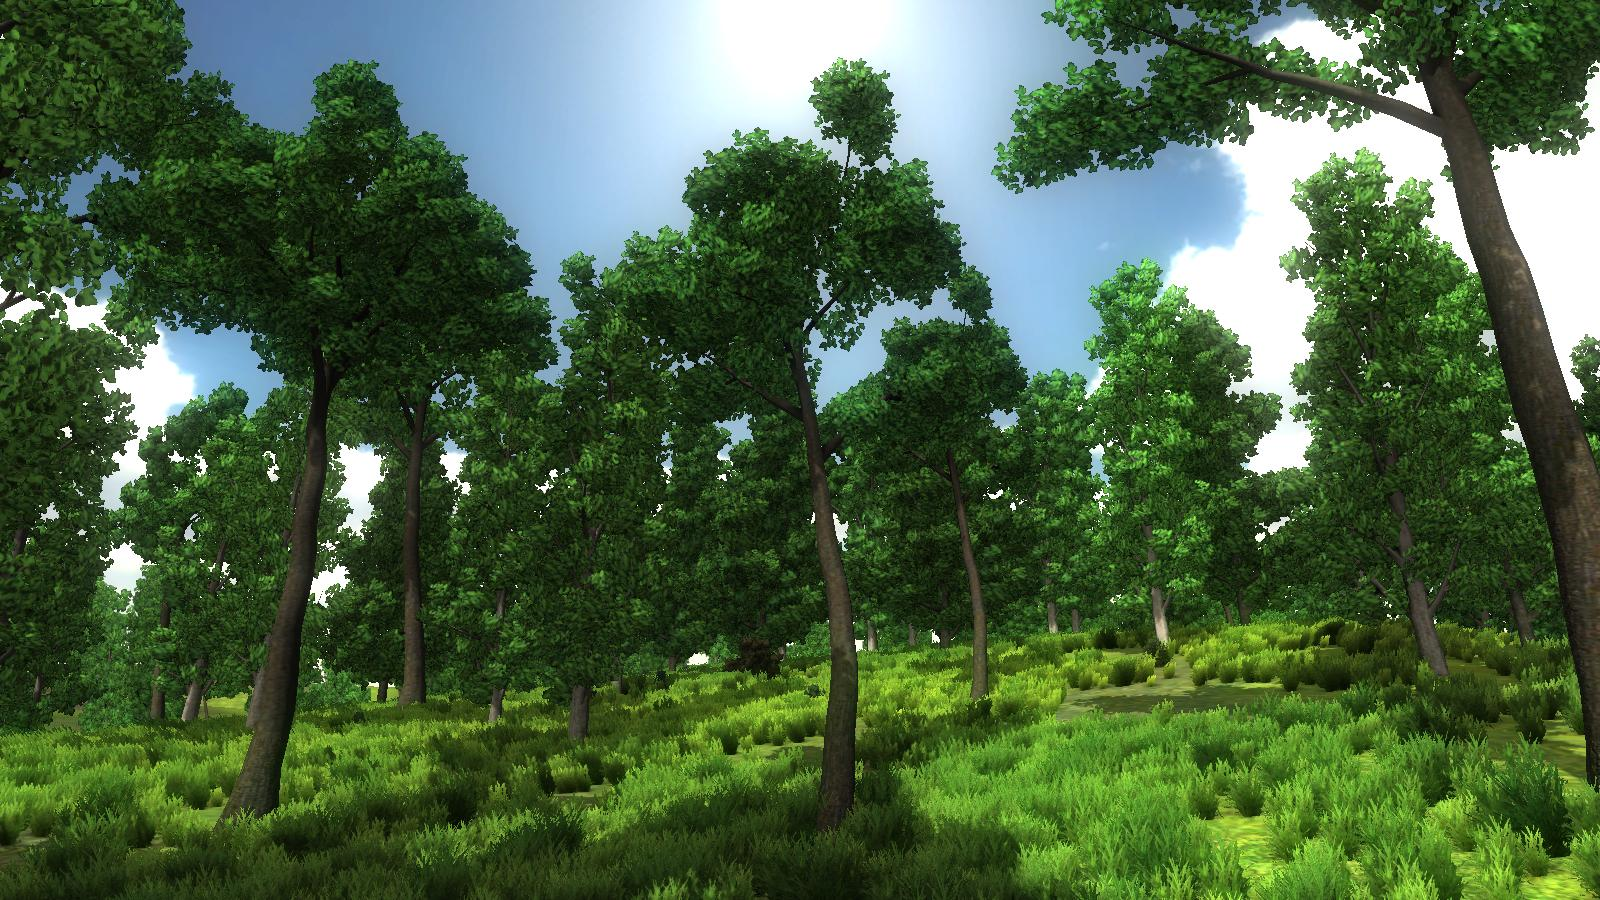
\includegraphics[width=0.5\textwidth]{speedtree}
\caption{SpeedTree}
\label{fig:speedtree}

\end{figure}

\begin{figure}

\centering
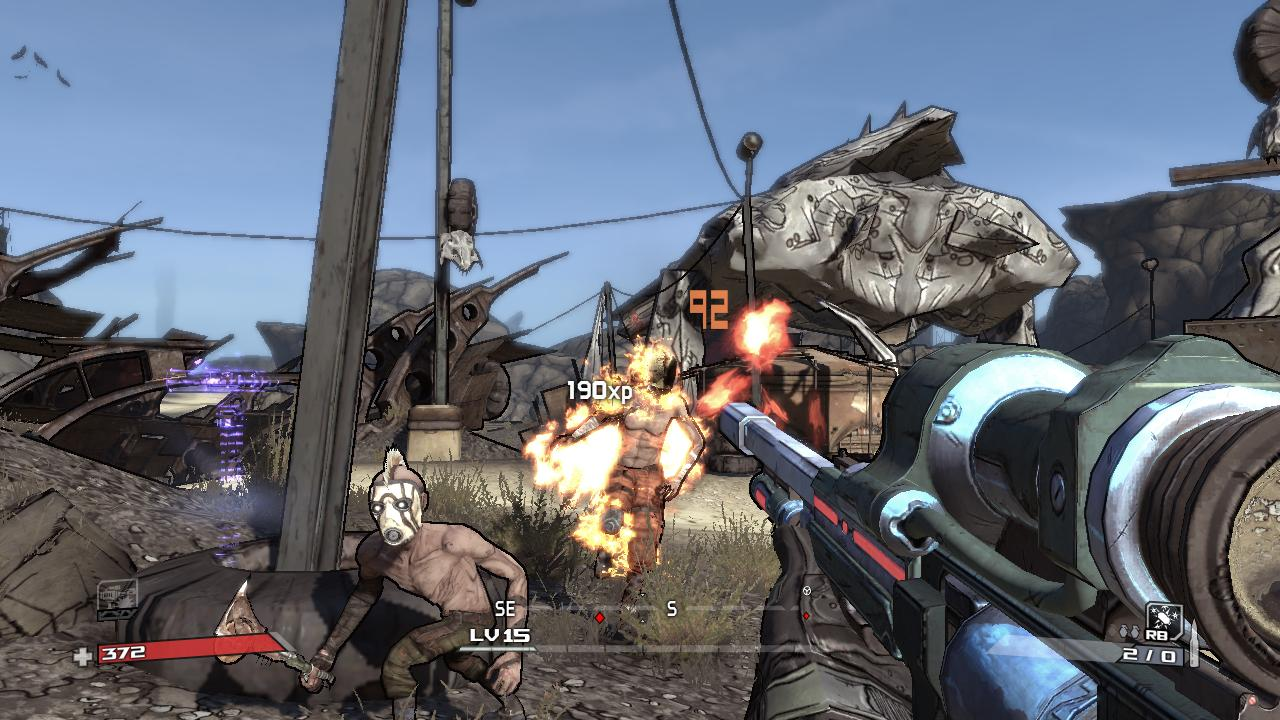
\includegraphics[width=0.5\textwidth]{borderlands}
\caption{Borderlands}
\label{fig:borderlands}

\end{figure}

\section{Tassonomia}

Il campo della PCG comprende molte tecniche e algoritmi che sono stati sviluppati sia ricerca accademica sia dall'industria.
Per descrivere in dettaglio come si suddivide questo campo di ricerca, andremo a usare la tassonomia introdotta dal lavoro
di Togelius et al. \cite{taxonomy:article}.

\paragraph{Online o Offline:}
La generazione procedurale può avvenire \emph{online} o \emph{offline}.
\emph{Online} significa generare contenuto in tempo reale durante il gioco, ma questo richiede una elevata efficienza computazionale data la necessità di generare il contenuto nel minor tempo possibile.
\emph{Offline} invece vuol dire generare contenuti prima che sia avviato il gioco; questo ovviamente non impone limiti di tempo, ma una volta generato il contenuto, questo non può essere cambiato.
 
\paragraph{Contenuto necessario o opzionale:}
Nei videogiochi possiamo avere dei contenuti necessari o opzionali.
Tutto ciò che è importante ai fini del gameplay, per esempio le armi in un sparatutto in prima persona, 
sono contenuti necessari, e devono essere funzionanti. Ciò comporta che se il contenuto necessario deve essere 
generato dalla PCG, questo deve sottostare a requisiti di qualità molto stretti, e quindi restringiamo le possibilità offerte dalla generazione procedurale.
Invece tutto quello che riguarda aspetti opzionali o marginali in un gioco, come per esempio gli alberi di una foresta,
possono essere più flessibili a livello di generazione, in quanto hanno requisiti meno stringenti.
 
\paragraph{\emph{Random seed} o vettore di parametri:}
Il game designer può avere più o meno controllo rispetto a ciò che viene prodotto dalla PCG.
Infatti è possibile creare contenuto solo partendo da un \emph{seed} che inizializzi l'algoritmo,
come per esempio nella generazione procedurale di labirinti.
Se invece è necessario avere un controllo maggiore sul contenuto generato,
allora vengono usati dei vettori di parametri che vanno a restringere il campo di ricerca dell'algoritmo,
in modo tale che il contenuto abbia certi requisiti imposti dal design del gioco.
 
\paragraph{Generazione stocastica o deterministica:}
Per la PCG possiamo avere algoritmi più o meno deterministici.
Questo è una decisione di design, cioè a seconda di che risultati si vogliono ottenere,
si possono usare algoritmi più deterministici nel caso si voglia essere certi dei risultati (con l'inconveniente
di avere una generazione meno flessibile), o meno deterministici, in modo da ottenere più varietà nel contenuto 
generato ma a costo di ottenere risultati potenzialmente peggiori dal punto di vista qualitativo.

\paragraph{\emph{Constructive} o \emph{Generate-and-test}:}
Gli algoritmi usati nella PCG possono essere divisi in due categorie: \emph{constructive} o \emph{generate-and-test}.
Il primo crea i contenuti direttamente attraverso dei processi \emph{ad-hoc} che garantiscano una certa qualità del contenuto generato.
Il secondo crea contenuti e poi li testa attraverso un criterio, umano o artificiale, definito dal designer dell'algoritmo.
I giochi commerciali preferiscono usare approcci \emph{constructive}, in genere più affidabili e quindi più adatti a prodotti con requisiti di qualità elevati,
mentre il secondo approccio ha una grande attenzione da parte della comunità accademica per le sue grandi potenzialità creative.

\subsection{Search Based Procedural Content Generation}
\label{sec:SBPCG}

Nell'ambito degli algoritmi di tipo \emph{generate-and-test} una grande rilevanza è data alla \emph{generazione di contenuti con algoritmi di ricerca}
(\emph{Search Based Procedural Content Generation}).
Questi usano tecniche di ricerca evolutive o euristiche per generare i contenuti. 
Questo tipo di generazione è caratterizzato da tre aspetti fondamentali: la rappresentazione, la funzione di fitness e l'algoritmo di ricerca.

\paragraph{Rappresentazione dei contenuti e lo spazio di ricerca:}
Per rappresentazione si intende come vengono rappresentati i contenuti, chiamati solitamente individui.
Per ogni individuo abbiamo due rappresentazioni: il \emph{genotipo} e il \emph{fenotipo}.
Il genotipo è una struttura dati che è usata dall'algoritmo di ricerca, mentre il fenotipo è usata nella fase di test e per l'implementazione finale del contenuto.
Per collegare le due rappresentazioni, si possono utilizzare due tipo di \emph{encoding}.
Nel \emph{direct encoding} abbiamo una mappatura diretta tra genotipo e fenotipo, cioè ogni elemento del genotipo ha una relazione 
lineare con la sua rappresentazione nel fenotipo.
Nel \emph{indirect encoding} invece esiste una relazione non lineare tra genotipo e fenotipo, il che comporta potenzialmente
un funzione di encoding più complessa, e quindi un peso maggiore a livello computazionale rispetto all'\emph{encoding} diretto.
Formalmente se prendiamo in considerazione i due insiemi , $X$ come l'insieme dei genotipi e $Y$ come l'insieme dei fenotipi, la funzione di \emph{encoding} è $ y = f(x) $, dove $ x \in X $ ,  $y \in Y $ e $ f: X \to Y.$
Una rappresentazione molto usata in letteratura per il genotipo vede l'uso di un vettore di numeri reali. Infatti questi possono essere facilmente implementati all'interno degli algoritmi di ricerca, e molto spesso riescono a formalizzare bene i contenuti utilizzati in questo tipo di problemi.
Però lo spazio di ricerca formalizzato da questi vettori deve possedere alcune caratteristiche importanti al fine di ottenere risultati coerenti e corretti.
La prima caratteristica è la dimensionalità:  vettori di dimensione troppo ridotta non riescono a rappresentare in modo corretto il contenuto, in quanto possono esserci caratteristiche indipendenti le une dalle altre che non possono essere codificate con un unico parametro, mentre se la dimensione del vettore diventa troppo grande lo spazio di ricerca può diventare troppo complesso per essere ricercato in modo esaustivo dall'algoritmo.
La seconda caratteristica è la località della rappresentazione: la rappresentazione deve garantire che per ogni piccola differenza nel genotipo sia corrisposta da una piccola differenza nel fenotipo. Questo principio può essere garantito più facilmente  con l'\emph{encoding} diretto, ma non è sempre possibile utilizzarlo, in quanto la scelta dell'\emph{encoding} dipende dal problema preso in considerazione.

\paragraph{Funzione di fitness:}
Per funzione di fitness intendiamo la valutazione dei contenuti che avviene nella fase di test.
Il design di questa funzione pone il seguente problema: stabilire cosa deve essere ottimizzato e 
in che modo formalizzarlo.
Abbiamo tre tipi di funzioni di fitness:
\begin{itemize}
\item Funzione di valutazione diretta: calcoliamo la fitness direttamente dal contenuto generato. Vengono estratte alcune caratteristiche d'interesse dal contenuto generato e in base a queste ne valutiamo la qualità. Un esempio può essere la dispersione delle risorse in una mappa per giochi di strategia, o il numero di percorsi presenti in un labirinto procedurale.
\item Funzione basata sulla simulazione: valutiamo il contenuto sulla base dei dati raccolti tramite un'intelligenza artificiale, che gioca a una parte del gioco. Molto spesso non è banale valutare il contenuto generato dall'algoritmo: una soluzione spesso usata è sviluppare un'intelligenza artificiale che prova il contenuto generato, e in base ai dati raccolti dalla simulazione, vengono valutati i contenuti. Un esempio può essere valutare il numero di uccisioni ottenuti in una mappa generata proceduralmente o giocare a un gioco da tavolo con nuove regole generate dall'algoritmo genetico.
\item Funzione interattiva: si coinvolge nella valutazione l'utente finale direttamente o indirettamente. Direttamente si intende una richiesta esplicita all'utente di cosa pensa del contenuto, mentre l'indiretta consiste nel 
raccogliere dati di una o più partite dell'utente e usare quanto raccolto per valutare la fitness. 
La valutazione diretta può essere complicata: infatti non è facile integrare con il gameplay delle richieste esplicite al giocatore; anche quando la valutazione è indiretta non è facile fare deduzioni sulla base dei dati, che inoltre possono essere soggetti a rumore, essere incompleti o poco affidabili.
\end{itemize}

\paragraph{Algoritmo:}
Una volta stabiliti la rappresentazione e la funzione di fitness, bisogna scegliere un algoritmo di ricerca.
Una scelta molto diffusa in letteratura sono gli algoritmi genetici (\emph{Genetic Algorithm} \cite{ga:article}).
Gli algoritmi genetici consistono in una ricerca euristica che imita i processi naturali di selezione, riproduzione, \emph{crossover} dei cromosomi e mutazione dei geni.
Per \emph{crossover} si intende un processo che dati due individui, ne produce due nuovi ottenuti attraverso la ricombinazione dei due \emph{genitori}.
La mutazione invece è una variazione causale dell'individuo.
Si possono trovare molte implementazione di questi due operatori, e la loro scelta è determinata dal problema da affrontare.

L'algoritmo può essere riassunto come segue:

\begin{enumerate}
 \item Viene generato un insieme casuale di individui (popolazione iniziale);
 \item Viene calcolata la fitness per ogni individuo della popolazione;
 \item I candidati per la prossima generazione vengono selezionati in base alla loro fitness;
 \item Gli individui selezionati vengono quindi usati per creare la nuova popolazione, con l'uso dei dei due operatori genetici.
 \item Si ripete dal punto 2 finché il numero desiderato di generazioni viene raggiunto.
\end{enumerate}

\section{PCG negli \emph{shooter}}

La generazione procedurale di contenuti con algoritmi di ricerca è stata applicata a numerose applicazioni; possiamo trovare esempi notevoli in molti e diversi generi videoludici.
Nei giochi di guida troviamo esempi nella generazione di tracciati, per esempio nel lavoro di Loiacono, Cardamone e Lanzi \cite{trackgen:article}, vengono generati tracciati con algoritmi evolutivi usando come funzione di fitness la diversità e le variazioni di velocità nell'affrontare il circuito.
Nei videogiochi a piattaforme (\emph{platform}), giochi in cui la meccanica principale consiste nell'attraversare i livelli saltando su delle piattaforme poste a differenti altezze, ci si è concentrati nella generazione della struttura dei livelli. Per esempio nell'articolo Michael Cook, Simon Colton, and Jeremy Gow\cite{platform:article} si propone l'utilizzo di \emph{algoritmi cooperativi e coevolutivi} per generare platform massimizzando un  funzione di fitness che codifica lo spazio raggiungibile dal giocatore nel livello generato.
Nei giochi strategici, giochi con visuale dall'alto in cui si controllano delle unità che possono essere utilizzate per raccogliere risorse o per attaccare l'avversario, troviamo l'uso della PCG per la generazione delle mappe. Un esempio è PSMAGE \cite{psmage:article}, un tool usato per generare mappe bilanciate per il gioco strategico \emph{Starcraft}
\footnote{\url{http://en.wikipedia.org/wiki/StarCraft}}.
Nei giochi \emph{rogue-like} e simili, giochi di ruolo caratterizzati da alcuni elementi comuni tra cui una sola vita a disposizione del giocatore e movimenti a turni, la generazione di labirinti è l'aspetto più importante. Nella letteratura possiamo trovare numerosi esempi, tra cui quello di Soreson e Pasquier \cite{dungeon:article}, dove si cerca di massimizzare la distanza tra ingresso e uscita del labirinto generato.
Per quanto riguarda il genere degli \emph{sparatutto in prima persona} (\emph{First Person Shooter}), la comunità accademica si è concentrata su due aspetti principali: la generazione di mappe e la generazione di armi.

\subsection{Generazione di mappe per FPS}
Negli \emph{sparatutto in prima persona} la mappe per le modalità multiplayer sono un aspetto fondamentale del gameplay.
Infatti delle mappe ben fatte ed equilibrate possono determinare il successo commerciale del gioco.
Quindi desta molto interesse la generazione automatica delle mappe attraverso le tecniche di PCG; ciò può permettere di ottenere un numero potenzialmente infinito di mappe e che soddisfino alcuni requisiti di gameplay, tra cui il bilanciamento.
Inoltre la generazione automatica può diminuire notevolemente i tempi di sviluppo di un FPS.

Nel lavoro condotto da Cardamone et al.\cite{fpsmaps:article} si propone una soluzione al problema basata su algoritmi di ricerca. 
In particolare si è cercato di creare automaticamente mappe per sessioni multigiocatore, cioè partite in cui diversi giocatori controllati da persone fisiche o dal computer 
combattono gli uni contro gli altri per raggiungere un determinato obiettivo; infatti esistono più tipi di modalità, per esempio nella modalità \emph{deathmatch} vince chi raggiunge per primo un numero prefissato di \emph{frag} (il numero di uccisioni di un giocatore), invece nella modalità \emph{capture the flag} vince la prima squadra di giocatori che riesce a portare alla sua base una bandiera presente nella mappa di gioco un determinato numero di volte.
Le mappe degli FPS sono caratterizzate da una serie di stanze collegate da corridoi e in questo ambiente vengono messi in posizioni strategiche delle risorse che possono essere raccolte dal giocatore (munizioni, armi o power-up). Inoltre queste possono svilupparsi in più piani, con la presenza di elevatori, scale, punti di ripristino, ecc.
Nell'esempio in analisi ci si è concentrati sulla modalità \emph{deathmatch} e su delle mappe a singolo piano.

Il loro obiettivo è stato quello di generare mappe \emph{interessanti}. Infatti le mappe che hanno più successo sono quelle che consentono ai giocatori di adottare diverse strategie di combattimento, ma che evitano il comparire di strategie dominanti, le quali possono rovinare l'esperienza di gioco.
Questo richiede l'utilizzo di un funzione di fitness che riesca formalizzare questo concetto.
\subsubsection{Funzione di fitness}
Come funzione di fitness hanno assunto che l'interesse verso una particolare mappa sia strettamente legato al \emph{fighting time} ( tempo di combattimento) del giocatore, $T_f$:
quanto tempo trascorre tra quando il giocatore comincia a giocare e quando viene ucciso.
Oltre a questo indice, hanno aggiunto un altro fattore: la quantità di spazio libero presente nella mappa. Questo è determinato dal fatto che se la mappa è troppo piccola, 
non c'è abbastanza spazio per posizionare le risorse, il che può portare a valori di \emph{fighting time} irrealistici.
Per calcolare $T_f$ hanno usato un approccio basato sulla simulazione: un gruppo di 4 giocatori controllati dall'intelligenza artificiale (bot) vengono fatti giocare per 10 minuti nella mappa presa in considerazione, e viene raccolto il tempo medio di combattimento per ciascun bot.
 
 
\subsubsection{Rappresentazione}
Per la rappresentazione sono state scelti quattro diversi approcci: \emph{All-White, All-Black, Grid, Random-Digger}.
Per quanto riguarda il fenotipo questo è identico in tutti e quattro gli approcci: la mappa viene rappresentata con una matrice di 64 x 64 celle.
Invece il genotipo cambia a seconda della rappresentazione (vedi figure \ref{fig:all_white_black} e \ref{fig:grind_digger}):
\begin{description}
\item[All-White:] mappa inizialmente vuota, vengono inseriti al suo interno i muri, ognuno dei quali viene rappresentato da una terna di valori $<x, y, l>$, dove
$x,y$ sono le coordinate mentre $l$ e la lunghezza del muro.
\item[All-Black:] mappa inizialmente piena di muri,  vengono inserite mano a mano stanze e corridoi; le stanze (quadrate) vengono rappresentate con la terna $<x, y, s>$ dove $x, y$ sono le coordinate del centro mentre $s$ è la dimensione del lato, i corridoi sono invece mappati dalla terna $<x, y, l>$, esattamente come nella rappresentazione \emph{All-White}.
\item[Grind:] la mappa viene rappresentata come una griglia di muri 9 x 9;  il genoma codifica quali muri per ogni quadrato sono attivi o meno, attraverso l'uso di un numero per ogni allele.
\item[Random-digger:] la mappa inizialmente è piena di muri, e un agente viene usato per  \emph{scavare} nei muri; il genoma codifica per ogni posizione nella mappa la probabilità dell'agente di scavare in una delle 4 direzioni possibili.
\end{description}
La rappresentazione \emph{Grind} utilizza quindi un \emph{encoding} diretto, mentre nelle altre tre rappresentazioni (\emph{All-White, All-Black} e in particolar modo \emph{Random-Digger}) abbiamo un \emph{encoding} indiretto.

\begin{figure}
\centering
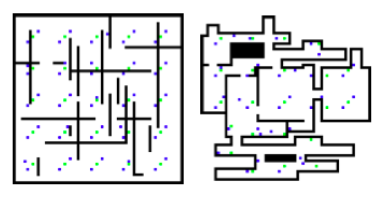
\includegraphics[width=0.5\textwidth]{all_white_black}
\caption{A sinistra mappa generata con rappresentazione All-White, a destra con All-Black}
\label{fig:all_white_black}
\end{figure}

\begin{figure}
\centering
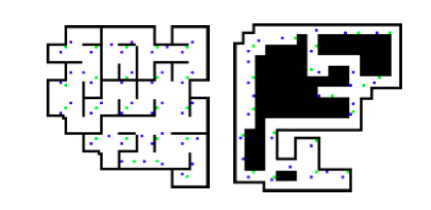
\includegraphics[width=0.5\textwidth]{grind_digger}
\caption{A sinistra mappa generata con rappresentazione Grind, a destra con Random-Digger}
\label{fig:grind_digger}
\end{figure}

\subsubsection{Risultati}
I risultati hanno evidenziato che a seconda della rappresentazione emergono diverse caratteristiche:
\begin{itemize}
\item Random-Digger crea lunghi corridoi e piccole stanze;
\item All-Black genera grandi arene e corridoi molto corti;
\item Grid genera mappe molto interessanti e simmetriche;
\item All-White genera le mappe con la fitness più alta;
\end{itemize}
Dai risultati si evince che la fitness più alta è appunto ottenuta con la rappresentazione All-White: questo probabilmente è dovuto alla combinazione di passaggi molto stretti e grandi arene, che permette ai bot di nascondersi e intrappolare gli avversari.

\subsubsection{Estensioni}
Il lavoro di Cardamone è stato poi esteso dal lavoro di Lanzi, Loiacono e Stucchi \cite{stucchi:article}.
Qui partendo dalle basi del lavoro precedente si è cercato di ottenere delle mappe che massimizzassero il bilanciamento dei combattimenti tra due giocatori a partire da una situazione di svantaggio per uno dei due giocatori.
Quindi è stata utilizzata una diversa funzione di fitness, indice di quanto le uccisioni dei due bot siano bilanciate ($Uccisioni_{giocatore_1} = Uccisoni_{giocatore_2}$);
mentre per la rappresentazione sono stati usati i medesimi approcci del lavoro di Cardamone.
Dai risultati è emerso che utilizzando una rappresentazione \emph{All-Black} e dotando entrambi i bot di un'arma \emph{rifle}(mitragliatore) e impostando le loro abilità con valori differenti, si riesce ad evolvere una mappa che riesce a bilanciare la partita in modo efficace, con un incremento costante durante le generazioni. Ciò è dovuto alla presenza di corridoi che circondano un un'area aperta: questi permettono al bot con abilità minore di compensare il suo svantaggio, grazie agli spazi ristretti che gli consentono di prendere la mira più velocemente (vedi figura \ref{fig:grind_digger_stucchi}).

\begin{figure}
\centering
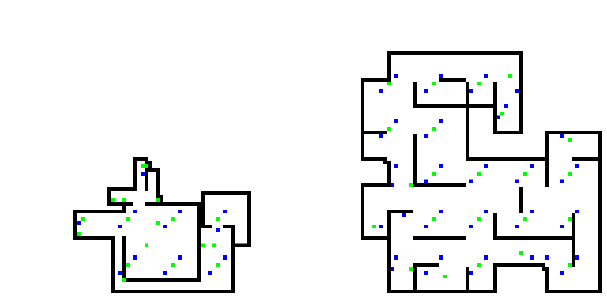
\includegraphics[width=1.0\textwidth]{stucchi_best}
\caption{A sinistra mappa migliore ottenuta con rappresentazione \emph{All-Black}, a destra con rappresentazione \emph{Grid}}
\label{fig:grind_digger_stucchi}
\end{figure}

\subsection{Generazione di armi per FPS}

La generazione di armi è un ancora un campo abbastanza inesplorato nel panorama della generazione procedurale di contenuti.

Come abbiamo già accennato, \emph{Borderlands} è un FPS dove le armi vengono generate proceduralmente, attraverso una combinazione di vari parametri.
Questi generano armi che rientrano in determinate categorie, tra cui pistole, mitragliatori, lanciagranate, fucili da assalto, fucili da cecchino, ecc.
Le generazione però non può generare armi innovative, in quanto la generazione è vincolata ai tipi di classe scelti dagli sviluppatori.

Invece in letteratura possiamo trovare alcuni esempi di generazione di armi che hanno posto l'accento sulla creatività del contenuto generato.
Questi sono \emph{Galactic Arm Race} e \emph{Team Blockhead Wars}.

\subsubsection{Team Blockhead Wars}
\emph{Team Blockhead Wars} (TBHW) \cite{tbhw:article} è un gioco sparatutto in prima persona (vedi figura \ref{fig:tbhw}), in cui si è tentato di generare le armi attraverso la modifica (\emph{tuning}) dei parametri delle armi,
mediante una funzione obiettivo basata su il tempo trascorso dal giocatore con l'arma generata.
TBHW usa un \emph{encoding diretto}, in quanto il genotipo (le variabili del genoma) è direttamente legato al fenotipo (parametri dell'arma); inoltre la valutazione è basata sugli utenti ed è basata sui dati raccolti sulle statistiche di utilizzo degli utenti, quindi è una valutazione indiretta e interattiva.

\begin{figure}

\centering
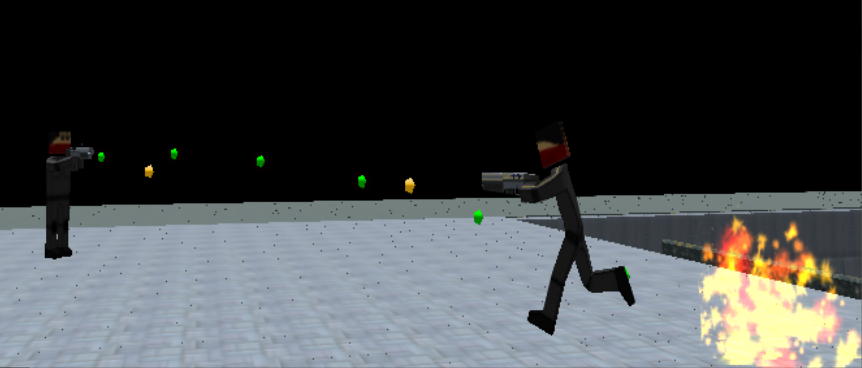
\includegraphics[width=1.0\textwidth]{TBHW_2}
\caption{Team Blockhead Wars, screenshot di un match}
\label{fig:tbhw}

\end{figure}

\subsubsection{Funzione di fitness}

La funzione di fitness è basata su due elementi:
\begin{itemize}
\item La quantità di tempo per cui l'arma generata è stata utilizzata;
\item Il numero di uccisioni che non siano suicidi ottenuti con l'arma;
\end{itemize}

\subsubsection{Rappresentazione}
Il genoma è un vettore di dieci parametri, scelti in modo da rappresentare il più possibile le caratteristiche generali di un'arma:
\begin{itemize}
\item Velocità -- velocità iniziale del proiettile;
\item Dimensioni -- raggio del proiettile;
\item Gravità -- gravità applicata al proiettile;
\item Danno -- danno causato dal proiettile;
\item Raggio -- raggio del danno causato quando il proiettile esplode;
\item Numero rimbalzi -- numero di rimbalzi del proiettile prima di esplodere;
\item Rateo di fuoco -- rateo di fuoco dell'arma;
\item Dimensioni del caricatore -- quanti proiettili si possono sparare prima di ricaricare;
\item Numero di munizioni -- massimo numero di munizioni per arma;
\item Tempo di ricarica -- tempo per ricaricare l'arma;
\end{itemize}
Ogni parametro ha dei limiti prefissati, oltre i quali non è possibile uscire durante l'evoluzione.

\begin{figure}
\centering
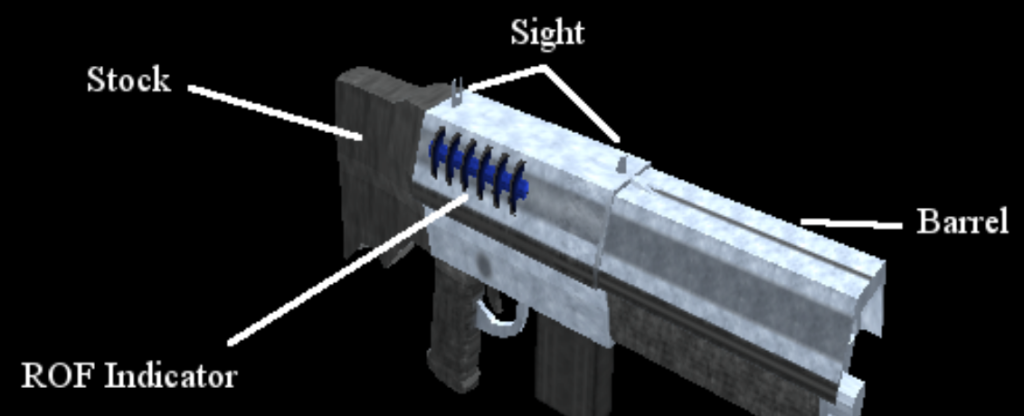
\includegraphics[width=1.0\textwidth]{TBHW_1}
\caption{Team Blockhead Wars, la mesh dell'arma cambia a seconda dei parametri}
\label{fig:tbhw}
\end{figure}

\subsubsection{Ciclo principale}
TBHW è un gioco costruito su un'architettura client-server, dove sul server viene lanciato l'algoritmo evolutivo mentre sui client gli utenti giocano al gioco e valutano le armi.
Ogni 10 minuti il server centrale crea una nuova generazione di armi e successivamente vengono inviate ai client.
Il giocatore può in ogni momento mettere in pausa il gioco, e selezionare due nuove armi.
Quindi una nuova popolazione viene così generata: 
\begin{enumerate}
\item Selezione degli individui proporzionale alla fitness dell'arma;
\item Crossover degli individui selezionati;
\item Mutazione degli individui selezionati;
\item Bilanciamento della nuova popolazione ottenuta;
\end{enumerate}
Come si può notare, è stata aggiunta una fase di bilanciamento, la quale ha lo scopo di bilanciare il rateo di danno di ciascun arma, per evitare di ottenere armi che massimizzassero tutti i parametri.
Dopo che l'arma è stata generata dall'algoritmo una nuova \emph{mesh} viene associata all'arma. 
Questa \emph{mesh} viene modificata per riflettere le caratteristiche intrinseche dell'arma: per esempio la canna dell'arma viene allungata proporzionalmente all'aumentare della velocità dei proiettili,
o il colore dei proiettili cambia a seconda di quanto danno infliggono.
Tutto questo per aiutare il giocatore a riconoscere le caratteristiche dell'arma, in quanto essendo la valutazione basata sul suo giudizio, è vitale che le potenzialità dell'arma siano comprese il più possibile dal giocatore.
\subsubsection{Risultati}
I risultati preliminari hanno mostrato dei risultati promettenti: l'algoritmo è stato capace di generare armi innovative e interessanti fin dai primi test.
Per esempio è stata generata un'arma con una velocità dei proiettili molto alta, e con un valore di rimbalzo pari a due; questo ha permesso i giocatori di usare tattiche innovative, come sparare verso un muro per colpire giocatori dall'altra parte della mappa attraverso il rimbalzo.
Un'altra arma interessante aveva proiettili con gravità bassa, danno molto alto e una capacità del caricatore molto alta, la quale si è dimostrata un'arma difensiva perfetta.

\subsubsection{Galactic Arm Race}

\emph{Galactic Arm Race} (GAR) \cite{gar:article} è un esperimento che utilizza un algoritmo evolutivo chiamato \emph{content-generating NeuroEvolution of Augmenting
Topologies (cgNEAT)}.
cgNEAT è una versione leggermente modificata di NEAT, un algoritmo per l'evoluzione di reti neurali , che vengono modificate aggiungendo o togliendo nodi e connessioni. Per una descrizione più dettagliata si rimanda all'articolo \cite{gar:article}.
cgNEAT usa NEAT per uno scopo diverso da quello per cui è nato: mentre NEAT viene usato per il controllo automatico, cgNEAT genera automaticamente dei pattern.
Infatti utilizzando sistemi particellari usati normalmente nella computer grafica e controllandoli con le reti neurali, si possono ottenere diversi pattern visivi.

GAR in particolare utilizza cgNEAT per generare proceduralmente delle armi. Infatti GAR è un gioco ambientato nello spazio (vedi figura \ref{fig:gar}), dove il giocatore controlla una navicella spaziale e il suo scopo è sconfiggere nemici, acquisire esperienza e raccogliere nuove armi. Queste vengono appunto rappresentate nel gioco dai sistemi particellari, che si differenziano in base al pattern dei proiettili, mentre la loro potenza rimane fissa qualunque sia l'arma generata.
Ogni giocatore possiede tre slot dove poter inserire le armi selezionate, e quando l'arsenale è pieno, il giocatore deve decidere quale arma scartare per poterne selezionare una nuova.
Ogni arma mostra nel mondo di gioco un'anticipazione del suo particolare pattern, in modo tale che il giocatore possa rendersi conto delle eventuali potenzialità dell'arma in questione.

\begin{figure}
\centering
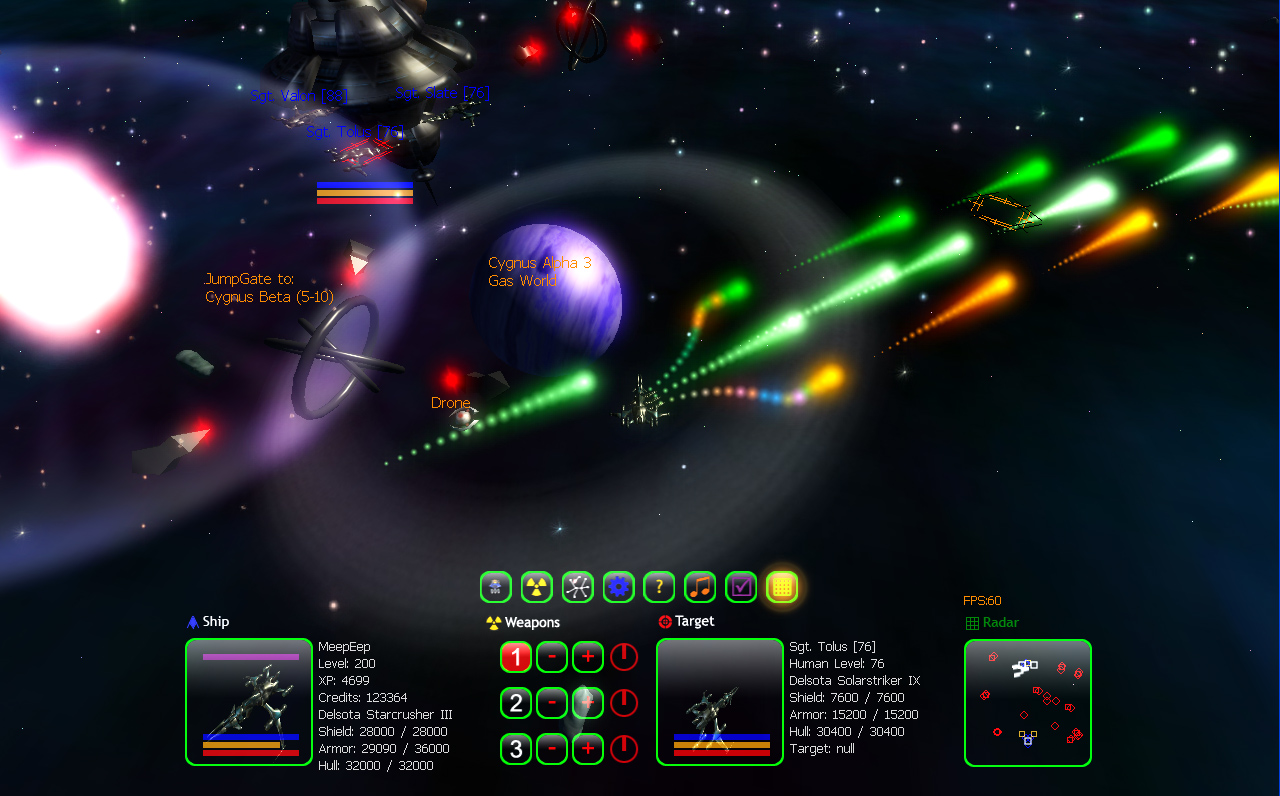
\includegraphics[width=1.0\textwidth]{GAR}
\caption{Screenshot di GAR}
\label{fig:gar}
\end{figure}

\subsubsection{Rappresentazione} 

\emph{Compositional Pattern Producing Network} sono una variazione delle reti neurali utilizzate da cgNEAT, dove l'insieme delle funzioni di attivazioni viene allargato, in modo tale da ottenere più tipi di pattern diversi; quindi per esempio oltre alle classiche funzioni gaussiane e sigmoid, vengono incluse anche funzioni lineari, periodiche ecc.
In questo modo, selezionando diversi tipi di funzione di attivazioni possono essere ottenuti diversi tipi di pattern (vedi figura ~\ref{fig:CPPN}).
Quindi usando come genotipo le CPPN e come fenotipo i sistemi particellari, abbiamo un \emph{encoding} indiretto.
Nel dettaglio la posizione della particella ($p_{x}$, $ p_{y}$) e la distanza dalla navicella del giocatore ($d_{c}$) vengono usati come input della CPPN, mentre l'output è usato per codificare la velocità delle particelle ($v_{x}$, $v_{z}$) e il loro colore ($r, g, b$).

\begin{figure} 
\centering
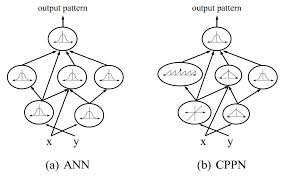
\includegraphics[width=0.5\textwidth]{CPPN}
\caption{Compositional Pattern Producing Network}
\label{fig:CPPN}
\end{figure}

\subsubsection{Funzione di fitness} 
La funzione di fitness è basata su quanto l'arma generata viene utilizzata dal giocatore.
Infatti quando viene selezionata la sua fitness incrementa in modo graduale, mentre quando viene deselezionata la sua fitness
gradualmente diminuisce, fino ad un minimo di uno.
La popolazione consta solo delle armi in possesso del giocatore, mentre quando vengono scartate queste vengono escluse dal
processo evolutivo.

\subsubsection{Ciclo principale}

Il ciclo principale è:

\begin{itemize}
\item All'inizio del gioco viene usata una popolazione prefissata, in modo tale che le armi iniziali garantiscano un minimo di usabilità. 
\item Il contenuto viene generato e posizionato nel mondo di gioco, ma non entra nel processo evolutivo finché non viene selezionato dal giocatore;
\item Nella fase riproduttiva, l'algoritmo seleziona i candidati in possesso del giocatore con un la \emph{roulette wheel}, basata sulla fitness descritta precedentemente; quindi vengono usati gli operatori genetici (crossover e mutazione) per produrre nuove CPPN;
\item Per preservare la diversità, c'è una certa probabilità che il contenuto generato venga prelevato da un insieme predefinito di contenuti già evoluti, detto \emph{spawning pool}.
\end{itemize}

Come si può notare, esistono alcune differenze dal processo evolutivo classico.
Il contenuto non è scartato direttamente dall'algoritmo, ma l'utente attivamente decide quali armi devono essere lasciate nella popolazioni e quali scartate; inoltre solo ciò che viene selezionato dal giocatore entra nel processo evolutivo, in modo da adattarsi alle preferenze dell'utente.

\subsubsection{Risultati} 
Sono stati effettuati alcuni test con il gioco, in particolare 10 giocatori hanno giocato a diverse partite con una durata minima di un'ora.
Durante questi test, sono trovate diverse armi innovative e interessanti.
Per esempio è stato trovato che i proiettili lenti possono bloccare efficacemente i proiettili avversari, mentre i proiettili più veloci sono efficaci sulle lunghe distanze.
Sono state generate anche armi con pattern che evolvono nel tempo, la velocità aumenta o diminuisce man mano che il pattern si sviluppa.
Inoltre per alcune classi di armi particolarmente interessanti sono stati assegnati dei nomi descrittivi della loro particolarità: per esempio i \emph{tunnel maker} sono armi che generano `tunnel' cioè creano due fasci di proiettili ai due lati del giocatore, mentre i \emph{wall makers} creano `muri' di proiettili in fronte alla navicella del giocatore (vedi figura \ref{fig:gar_2}).

\begin{figure}

\centering
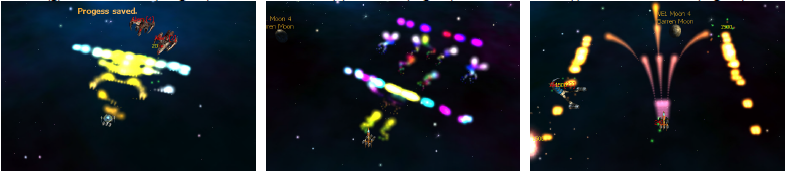
\includegraphics[width=1.0\textwidth]{gar-1}
\caption{Esempi di armi generati in GAR}
\label{fig:gar_2}

\end{figure}

\section{Sommario}
In questo capitolo abbiamo introdotto il concetto di Generazione procedurale di contenuti e gli algoritmi usati in questo campo.
Nella Sezione 2.1 abbiamo fatto un piccolo excursus storico della PCG e descritto alcuni tool e giochi commerciali che la utilizzano.
Nella Sezione 2.2 abbiamo introdotto il concetto di PCG applicato alla generazione di mappe per \emph{sparatutto}.
Nella Sezione 2.3 infine abbiamo descritto due esempi di generazione procedurale applicata alla produzione di armi negli shooter.

\chapter{Generazione automatica di armi bilanciate}

In questo capitolo andremo a descrivere gli obiettivi di questo lavoro e l'ambiente sviluppato per condurre gli esperimenti.
Nella prima parte andremo a descrivere i nostri obiettivi e il gioco usato per le simulazioni: Unreal Tournament III.
Nella seconda parte andremo a descrivere l'ambiente sviluppato per svolgere gli esperimenti e le modifiche apportate al gioco.

\section{Obiettivi}

L'obiettivo di questo lavoro è bilanciare automaticamente due armi attraverso la modifica dei parametri (\emph{tuning}).
Intuitivamente possiamo affermare che due armi sono equilibrate se mediamente ottengono lo stesso numero di uccisioni in una partita. 
Ma le armi non sono l'unico fattore determinante per una partita equilibrata: anche la mappa in cui si svolge la partita può influire notevolmente sull'esito del match.
Come abbiamo visto esistono già lavori che si sono concentrati nel generare mappe per FPS, dove si sottolinea l'importanza di avere mappe equilibrate per evitare strategie dominanti che rovinino l'esperienza di gioco.
Inoltre alcune mappe possono risultare equilibrate date due armi, ma non è detto che sia ugualmente un match equilibrato nel caso si scelgano altre due tipi di armi.
Per semplificare il problema abbiamo scelto una mappa già inclusa nel gioco, e l'abbiamo mantenuta costante per tutte le simulazioni, supponendo che la mappa fosse equilibrata qualunque siano le armi. Ovviamente questa è una semplificazione necessaria per svolgere il nostro lavoro, ma è possibile pensare di estendere questo lavoro in modo da generare contemporaneamente la mappa e le armi. 
Quindi abbiamo deciso di selezionare una mappa e di tenerla costante per tutte le nostre simulazioni, nelle quali cambieranno solo i parametri delle armi.
La simulazione si svolge nel seguente modo: due giocatori controllati dall'intelligenza artificiale del gioco vengono fatti combattere l'uno contro l'altro, ciascuno con un'arma fissa che non può essere sostituita durante tutta la durata della partita.
Quindi raccogliamo le statistiche delle uccisioni dei due bot: se il numero di uccisioni conseguite dal $bot_1$ è simile al numero di uccisioni ottenute dal $bot_2$ allora consideriamo le due armi equilibrate.
Questo impone il design di una funzione di fitness che formalizzi questo concetto.
Inoltre sono necessarie alcune considerazioni preliminari per decidere le abilità dei bot che simulano la partita, il numero di uccisioni massimo per partita e la durata della singola simulazione.
Ora descriveremo il gioco che abbiamo utilizzato per le simulazioni e successivamente descriveremo l'ambiente sviluppato per l'esecuzione degli esperimenti.

\section{Unreal Tournament III}
\emph{Unreal Tournament III} (UT3) è un gioco sviluppato dallo studio \emph{Epic Games}\footnote{\url{http://en.wikipedia.org/wiki/Unreal_Tournament_3)}}.
Sesto seguito della saga \emph{Unreal}, UT3 è uno sparatutto in prima persona, cioè un gioco in cui il giocatore impugna un'arma da una prospettiva in prima persona con l'obiettivo di sparare ai nemici (vedi figura \ref{fig:ut3}).
Nella modalità \emph{single player} si gioca contro l'intelligenza artificiale, mentre nella modalità \emph{multiplayer} si gioca contro altre persone connesse via rete.
Il multiplayer si suddivide ulteriormente in più modalità di gioco: nella modalità \emph{deathmatch} vince il giocatore che per primo raggiunge una determinata quantità di uccisioni, mentre nella modalità \emph{capture the flag} vince il primo team che riesce a riportare la bandiera della sua squadra alla propria base il maggior numero di volte prima che scada il tempo.
Esistono altre modalità, tra cui citiamo \emph{Warfare, Duel, Vehicle Capture the Flag, Betrayal and Greed}; per una loro descrizione rimandiamo al sito di Unreal Tournament III. 
Noi per questo lavoro abbiamo deciso di concentrarci sulla modalità \emph{deathmatch}.

UT3 è un gioco ambientato in un universo fantascientifico, dove troviamo un insieme di armi non realistiche che appartengono alle classi di armi che compaiono in tutti gli FPS, tra cui pistole, fucili a pompa, fucili da cecchino, fucili d'assalto, lanciamissili ecc.
L'engine usato da UT3 è l'\emph{Unreal Engine 3}\footnote{\url{http://en.wikipedia.org/wiki/Unreal_Engine_3)}}, sempre sviluppato da \emph{Epic Games}, con il quale sono stati sviluppati molti giochi commerciali degli ultimi anni grazie alla sua versatilità e una grafica ad alto impatto visivo.

Abbiamo deciso di usare questo engine per tre motivi principali: il primo è che permette di modificare facilmente la logica di gioco attraverso un linguaggio di \emph{scripting} chiamato \emph{UnrealScript}\footnote{\url{http://en.wikipedia.org/wiki/UnrealScript)}}; il secondo è che essendo un gioco sparatutto possiede già tutto il codice necessario per il funzionamento delle armi, il che ci ha permesso di apportare poche modifiche per adeguare il gioco ai nostri scopi; il terzo è che essendo UT3 un gioco commerciale che nasce sopratutto per la modalità a più giocatori, possiede un'avanzata intelligenza artificiale, che ci ha permesso di ottenere simulazione molto verosimili.

Inoltre il gioco può essere lanciato nella modalità \emph{Server}, il che permette di fare simulazioni senza \emph{rendering}, cioè senza che il gioco debba visualizzare la partita a schermo. Questo ci ha permesso di lanciare più partite contemporaneamente su un singolo computer, il che ha diminuito notevolmente i tempi necessari per ottenere i risultati.

\begin{figure}
\centering
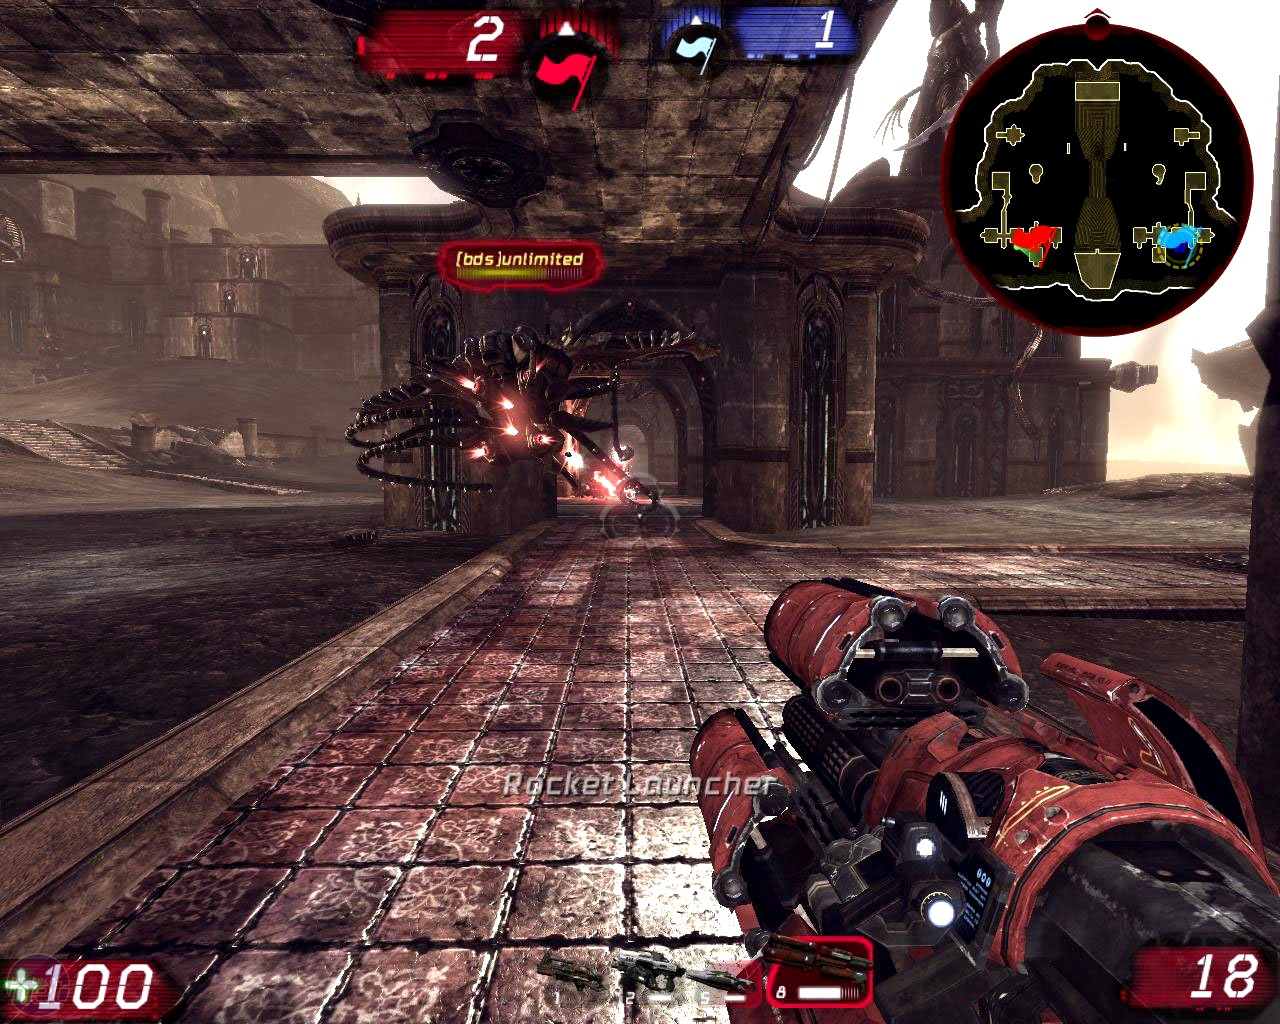
\includegraphics[width=1.0\textwidth]{UT3}
\caption{Unreal Tournament III}
\label{fig:ut3}
\end{figure}

\section{Ambiente simulativo}
\label{sec:setting}
Per calcolare il bilanciamento di due armi abbiamo bisogno di simulare una partita nel gioco UT3, e raccogliere le statistiche necessarie al calcolo del bilanciamento.
Per questo motivo abbiamo costruito un'architettura client-server, nella quale il gioco viene visto come server su cui lanciare le simulazioni, mentre il client manda i dati relativi per configurare la simulazione e riceve i risultati ottenuti dalle simulazioni effettuate.
Quindi abbiamo dovuto implementare in UT3 la simulazione tra due giocatori controllati dall'intelligenza artificiale e una rappresentazione delle armi tale che fosse abbastanza generale da poter rappresentare un vasto insieme di armi.

\subsection{Parametrizzazione delle armi}
Le armi presenti nel gioco Unreal Tournament III sono molto diverse le une dalle altre, in quanto possono includere diverse funzionalità e modalità di uso.
Per questo abbiamo deciso di estrarre le caratteristiche principali che ci permettessero di rappresentare il più possibile l'insieme di armi presenti negli giochi sparatutto in prima persona.
Abbiamo quindi deciso un numero di parametri pari a 10, che vengono descritti nella tabella \ref{tab:parametri}\footnote{Unreal Unit (UU) , citato nelle tabelle, è l'unità fondamentale di misura di lunghezza in UT3, e corrispondono a 2 cm reali}.

\begin{table}[htp]
\caption{Descrizione dei parametri}
\label{tab:parametri}
\centering
	 \begin{tabularx}{\textwidth}{lX}
	\toprule
	Parametro & Descrizione \\
	\midrule
	\textbf{Rate of Fire} & Frequenza di fuoco dell'arma, calcolato come numero di spari per secondo \\
	\midrule
	\textbf{Spread} & Numero puro che rappresenta l'errore aggiunto alla direzione dei proiettili quando questi vengono sparati\\
	\midrule
	\textbf{ShotCost} &  Numero di proiettili sparati contemporaneamente per ogni sparo dell'arma\\
	\midrule
	\textbf{LifeSpan} &  Tempo di `vita' del proiettile, cioè per quanto tempo rimane in gioco una volta che viene sparato\\
	\midrule
	\textbf{Speed} &  Velocità iniziale del proiettile quando viene sparato, calcolata come \emph{Unreal Unit} per secondo\\
	\midrule
	\textbf{Damage} &  Numero puro che rappresenta il danno causato all'avversario; questo numero indica numericamente quanta \emph{vita} viene tolta all'avversario: la \emph{vita} è un numero che rappresenta la vita del giocatore,
				    numero che varia da 100 (vita massima) a 0 (vita minima), e nel caso raggiunga il valore 0, il giocatore è considerato \emph{ucciso} dall'avversario che l'ha colpito\\
	\midrule
	\textbf{Damage Radius } & Raggio sferico del proiettile, calcolato in \emph{Unreal Unit}; i proiettili vengono rappresentati con delle sfere di raggio variabile e nel caso questa sfera intersechi il corpo dell'avversario, quest'ultimo viene 					                      danneggiato dal proiettile\\
	\midrule
	\textbf{Gravity } &   Gravità subita dal singolo proiettile; i proiettili sparati nel modo di gioco subiscono un'accelerazione sull'asse z costante, che può anche essere opposta rispetto alla gravità reale\\
	\midrule
	\textbf{Explosive} &   Raggio del danno esplosivo quando il proiettile esplode; i proiettili quando colpiscono un oggetto nel mondo di gioco provocano un'esplosione di raggio variabile, determinato da questo parametro e qualsiasi giocatore                				       che venga investito dal raggio esplosivo, anche il giocatore che ha sparato lo stesso proiettile, viene danneggiato di una quantità dipendente dal danno del proiettile\\
	\bottomrule
	\end{tabularx}
\end{table}
Tutti i parametri hanno un certo intervallo stabilito a priori (vedi tabella \ref{tab:limiti}), i quali vanno a limitare il campo di ricerca verso armi potenzialmente interessanti.

\begin{table}[htp]
\caption{Intervalli prefissati dei parametri delle armi e unità di misura}
\label{tab:limiti}
\centering
	\begin{tabular}{lrrr}
	\toprule
	Parametro & Minimo & Massimo & Unità Di Misura\\
	\midrule
	Rate Of Fire & 0 & 4 & $spari/secondo$\\
	Spread & 0 & 3 & numero puro \\
	ShotCost & 1 & 9 & numero proiettili\\
	LifeSpan & 0 & 100 & $secondi$\\
	Speed & 0 & 10000 & $UU/secondo$\\
	Damage & 0 & 100 & numero puro\\
	Damage Radius & 0 & 100  & $UU$\\
	Gravity & -250 & 250 & $UU/secondo^2$\\ 
	Explosive & 0 & 300  & $ UU $\\
	\bottomrule
	\end{tabular}
\end{table}

Andiamo inoltre a suggerire all'intelligenza artificiale alcune caratteristiche dell'arma, in modo tale che possa utilizzarla nel miglior modo possibile:
\begin{itemize}
\item \textbf{Fast Repeater} -- booleano che suggerisce al bot di usare l'arma per lunghe sequenze di colpi o meno;  viene impostato nel caso il \emph{Rate of Fire} dell'arma sia minore a $0.5$;
\item \textbf{Weapon Range} -- suggerisce al bot il raggio ottimale a cui usare l'arma, che nel caso la gravità sia diversa da zero viene calcolato come moto parabolico data la velocità iniziale e la gravità, mentre se la gravità è zero viene calcolato moltiplicando il \emph{LifeSpan} del proiettile per la sua velocità iniziale;
\item \textbf{Sniping} -- booleano che suggerisce di usare l'arma come se fosse un fucile da cecchino; viene impostato nel caso il parametro \emph{Weapon Range} sia maggiore di 2000 UU. 

\end{itemize}

\subsection{Simulazione delle partite}
\label{sec:simulation}
Nelle simulazioni vogliamo simulare una partita in modalità \emph{Deatmatch}, tra due giocatori, con un numero di uccisioni totali prefissato e un tempo limite.
Quindi abbiamo modificato la logica di gioco per poter simulare un match tra due giocatori controllati dall'intelligenza artificiale, a cui vengono assegnate due armi che non possono essere cambiate durante tutto l'arco di durata della partita.
Abbiamo deciso di sviluppare un'architettura client-server, nella quale il server offre come servizio una simulazione, e una volta dati come input i parametri delle armi e la configurazione della partita, il server restituisce al richiedente i risultati della partita dopo aver terminato la simulazione.

In generale una simulazione è costituita dai seguenti passi:
\begin{enumerate}
\item Il client che vuole testare due armi invia al server (su cui è stata lanciata la simulazione) i parametri delle due armi, la durata della partita e il \emph{goal score};
\item Il server riceve la configurazione della partita e parametri delle armi;
\item La partita viene inizializzata secondo la configurazione ricevuta e ai due bot vengono assegnate due nuove armi con i parametri inviati dal client;
\item Viene eseguita la simulazione;
\item La partita termina e i risultati della partita vengono inviati al client;
\item Il server si mette in attesa di ricevere una nuova richiesta dal client;
\end{enumerate}

Una volta terminata la simulazione, il server invia al client le seguenti statistiche della partita:
\begin{itemize}
\item Il numero di uccisioni delle due armi;
\item Il numero di morti delle due armi, che possono differire rispetto alle uccisioni a causa dei suicidi;
\item La media dei tempi che intercorrono tra quando un proiettile viene sparato e quando questo colpisce l'avversario, per entrambi le armi.
\item La media della distanze coperte dai proiettili tra quando un proiettile viene sparato e quando questo colpisce l'avversario, per entrambi le armi.
\item La media delle sequenze di uccisioni senza interruzioni eseguite dai due bot (\emph{kill streak}).
\end{itemize}
Le prime due statistiche vengono utilizzate per calcolare il bilanciamento, mentre le ultime tre per valutare alcune caratteristiche secondarie delle armi, il cui scopo verrà descritto nel capitolo 6.

Il match simulato termina quando la somma delle uccisioni ottenute dai due bot raggiunge un valore pari al \emph{goal score} o quando la durata della partita raggiunge il tempo limite impostato per la partita.
Il \emph{goal score} e il tempo limite sono due parametri di configurazione della partita che vengono inviati dal client al server, e quindi possono essere cambiati a seconda delle necessità.
Invece abbiamo altri due parametri di configurazione che sono fissi per tutte le simulazioni, e che sono stati impostati direttamente nel codice di gioco delle simulazioni: la mappa di gioco e l'abilità dell'intelligenza artificiale.
La mappa è \emph{DM-Biohazard}, un mappa di piccole dimensioni che si sviluppa sue due piani. \`E stata scelta tra le mappe disponibili del gioco in quanto le sue dimensioni ridotte sono ideali per simulare una partita tra due giocatori.
L'abilità dell'intelligenza artificiale può essere impostata con diversi livelli di abilità, rappresentati da un intervallo numerico compreso tra 0 e 7, dove al crescere del numero abbiamo un'abilità crescente: noi abbiamo deciso di impostare il livello di abilità massimo (7), in quanto ci interessava avere dei bot che simulassero un partita tra due giocatori esperti; oltretutto questo comporta un numero di uccisioni maggiori in un tempo minore.

Ora andremo a descrivere alcuni test preliminari atti a decidere in modo empirico come impostare la velocità delle simulazioni e il valore del \emph{goal score}.

\subsection{Velocità e durata delle simulazioni}
Come abbiamo detto precedentemente, per calcolare il bilanciamento delle armi abbiamo bisogno di simularle all'interno del gioco UT3.
Ogni simulazione richiede una certa quantità di tempo per essere eseguita. Come vedremo nei capitolo successivi, abbiamo bisogno di eseguire per ogni prova degli esperimenti un numero di simulazioni pari a 500, quindi abbiamo bisogno di ridurre al minimo i tempi richiesti per simulazione, in modo da ottenere dei tempi ragionevoli per gli esperimenti che andremo ad eseguire.
La durata complessiva delle simulazioni è determinata da tre parametri: la velocità a cui viene eseguito il gioco, il \emph{goal score} e il tempo limite delle partite.

\subsubsection{Velocità delle simulazioni}
In UT3 è possibile modificare la velocità a cui viene eseguito il gioco. Infatti la logica di gioco viene eseguita a una certa velocità, impostata in modo tale che sia verosimile rispetto al reale trascorrere del tempo.
Noi siamo interessati ad ottenere i risultati delle simulazioni nel minor tempo possibile, e dal momento che il gioco può essere eseguito nella modalità \emph{server}, cioè senza \emph{rendering} del gioco, abbiamo aumentato la velocità di gioco. Infatti in UT3 è possibile modificare la velocità attraverso un parametro chiamato \emph{GameSpeed}, il cui massimo incremento consentito è pari a 12 volte la velocità normale.
Purtroppo il gioco non è stato pensato per essere eseguito a queste velocità, quindi non è garantito che eseguendolo con l'incremento massimo la logica di gioco relativa all'intelligenza artificiale venga effettivamente chiamata con una frequenza più alta. Dal momento che le statistiche di gioco dipendono direttamente dal funzionamento dei bot, abbiamo la necessità che l'IA funzioni correttamente.
Infatti normalmente l'IA è una parte di logica che normalmente ha una prorità minore rispetto ad altri sezioni, come per esempio la simulazione della fisica di gioco.
Per questo motivo la frequenza con cui viene eseguita l'intelligenza artificiale può variare a seconda delle performance del gioco, e quindi può capitare che questa non venga eseguita con una frequenza maggiore se la velocità del gioco è troppo alta.
Quindi abbiamo condotto dei test per verificare con quale incremento avessimo i tempi migliori di simulazione. Dal momento che gli esiti della simulazione sono influenzati anche dal tipo di armi usate, abbiamo svolto la nostra analisi usando tre diverse coppie di armi per ridurre tale dipendenza nei risultati ottenuti.
Abbiamo lanciato 10 simulazioni per ogni coppia di armi , e abbiamo raccolto i risultati.

\begin{figure}[htp]
\centering
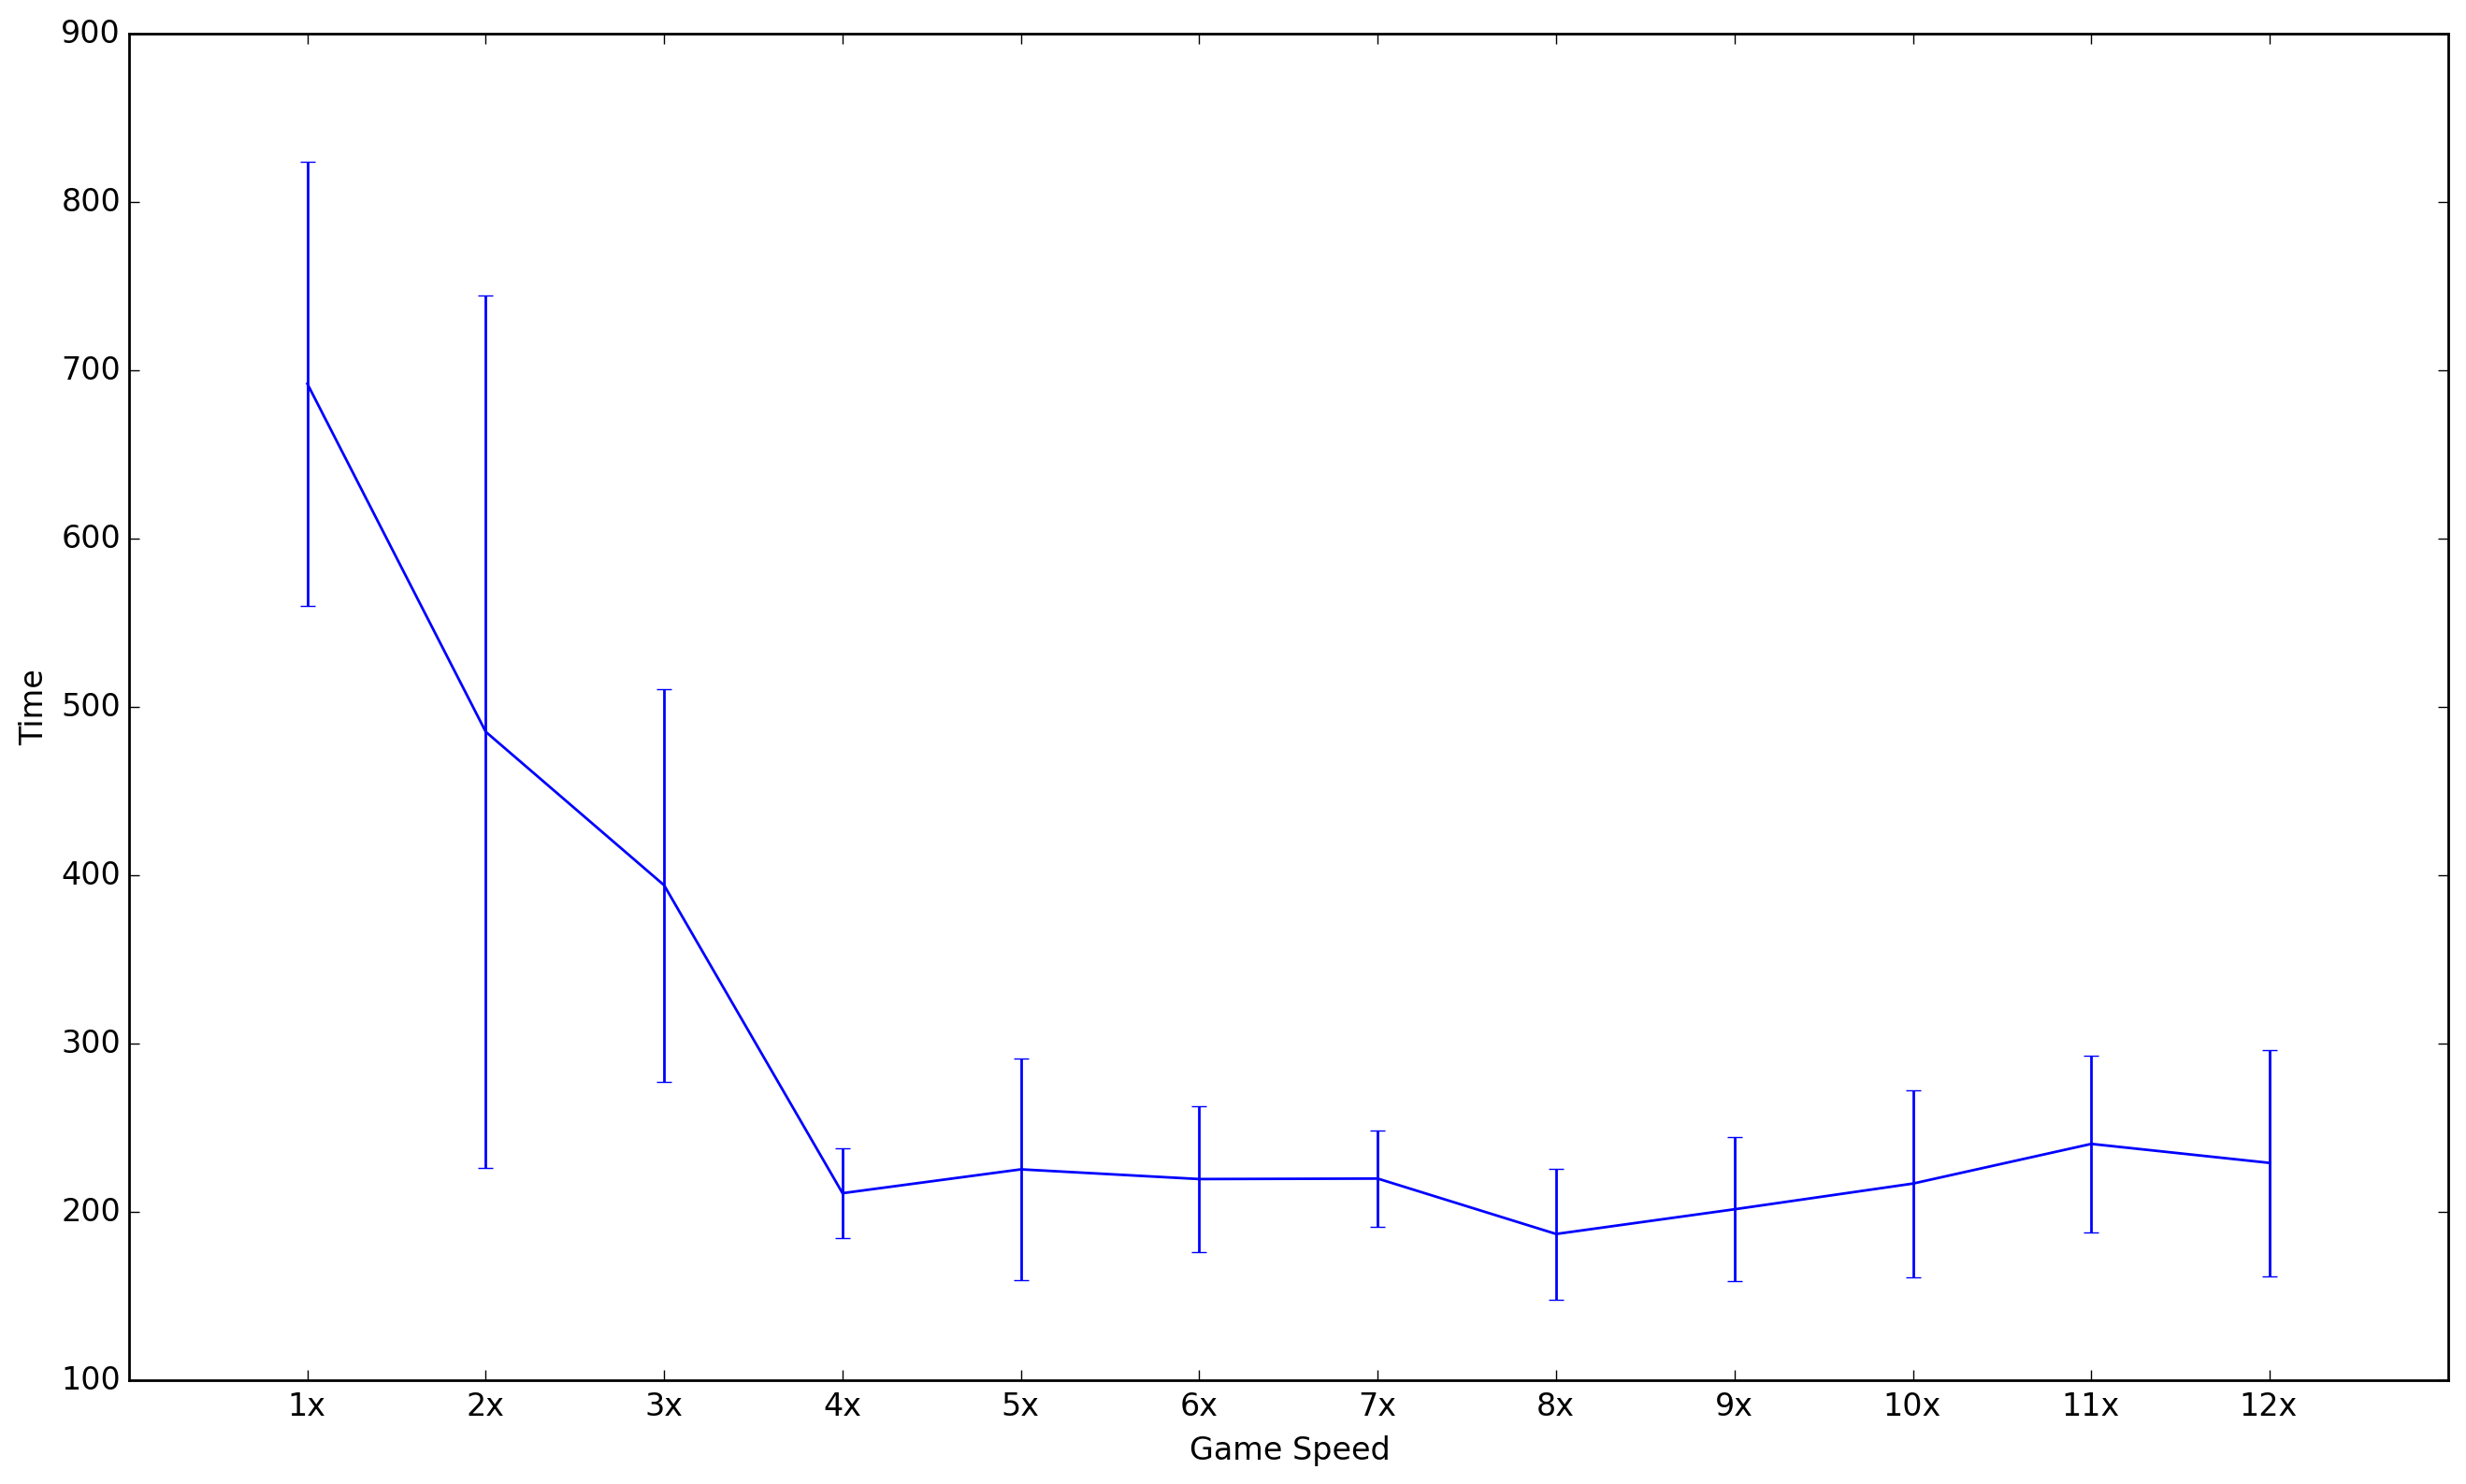
\includegraphics[width=1.0\textwidth]{time_speed_1}
\caption{Tempi delle simulazioni con la prima coppia di armi}
\label{fig:time_speed_1}
\end{figure}

\begin{figure}[htp]
\centering
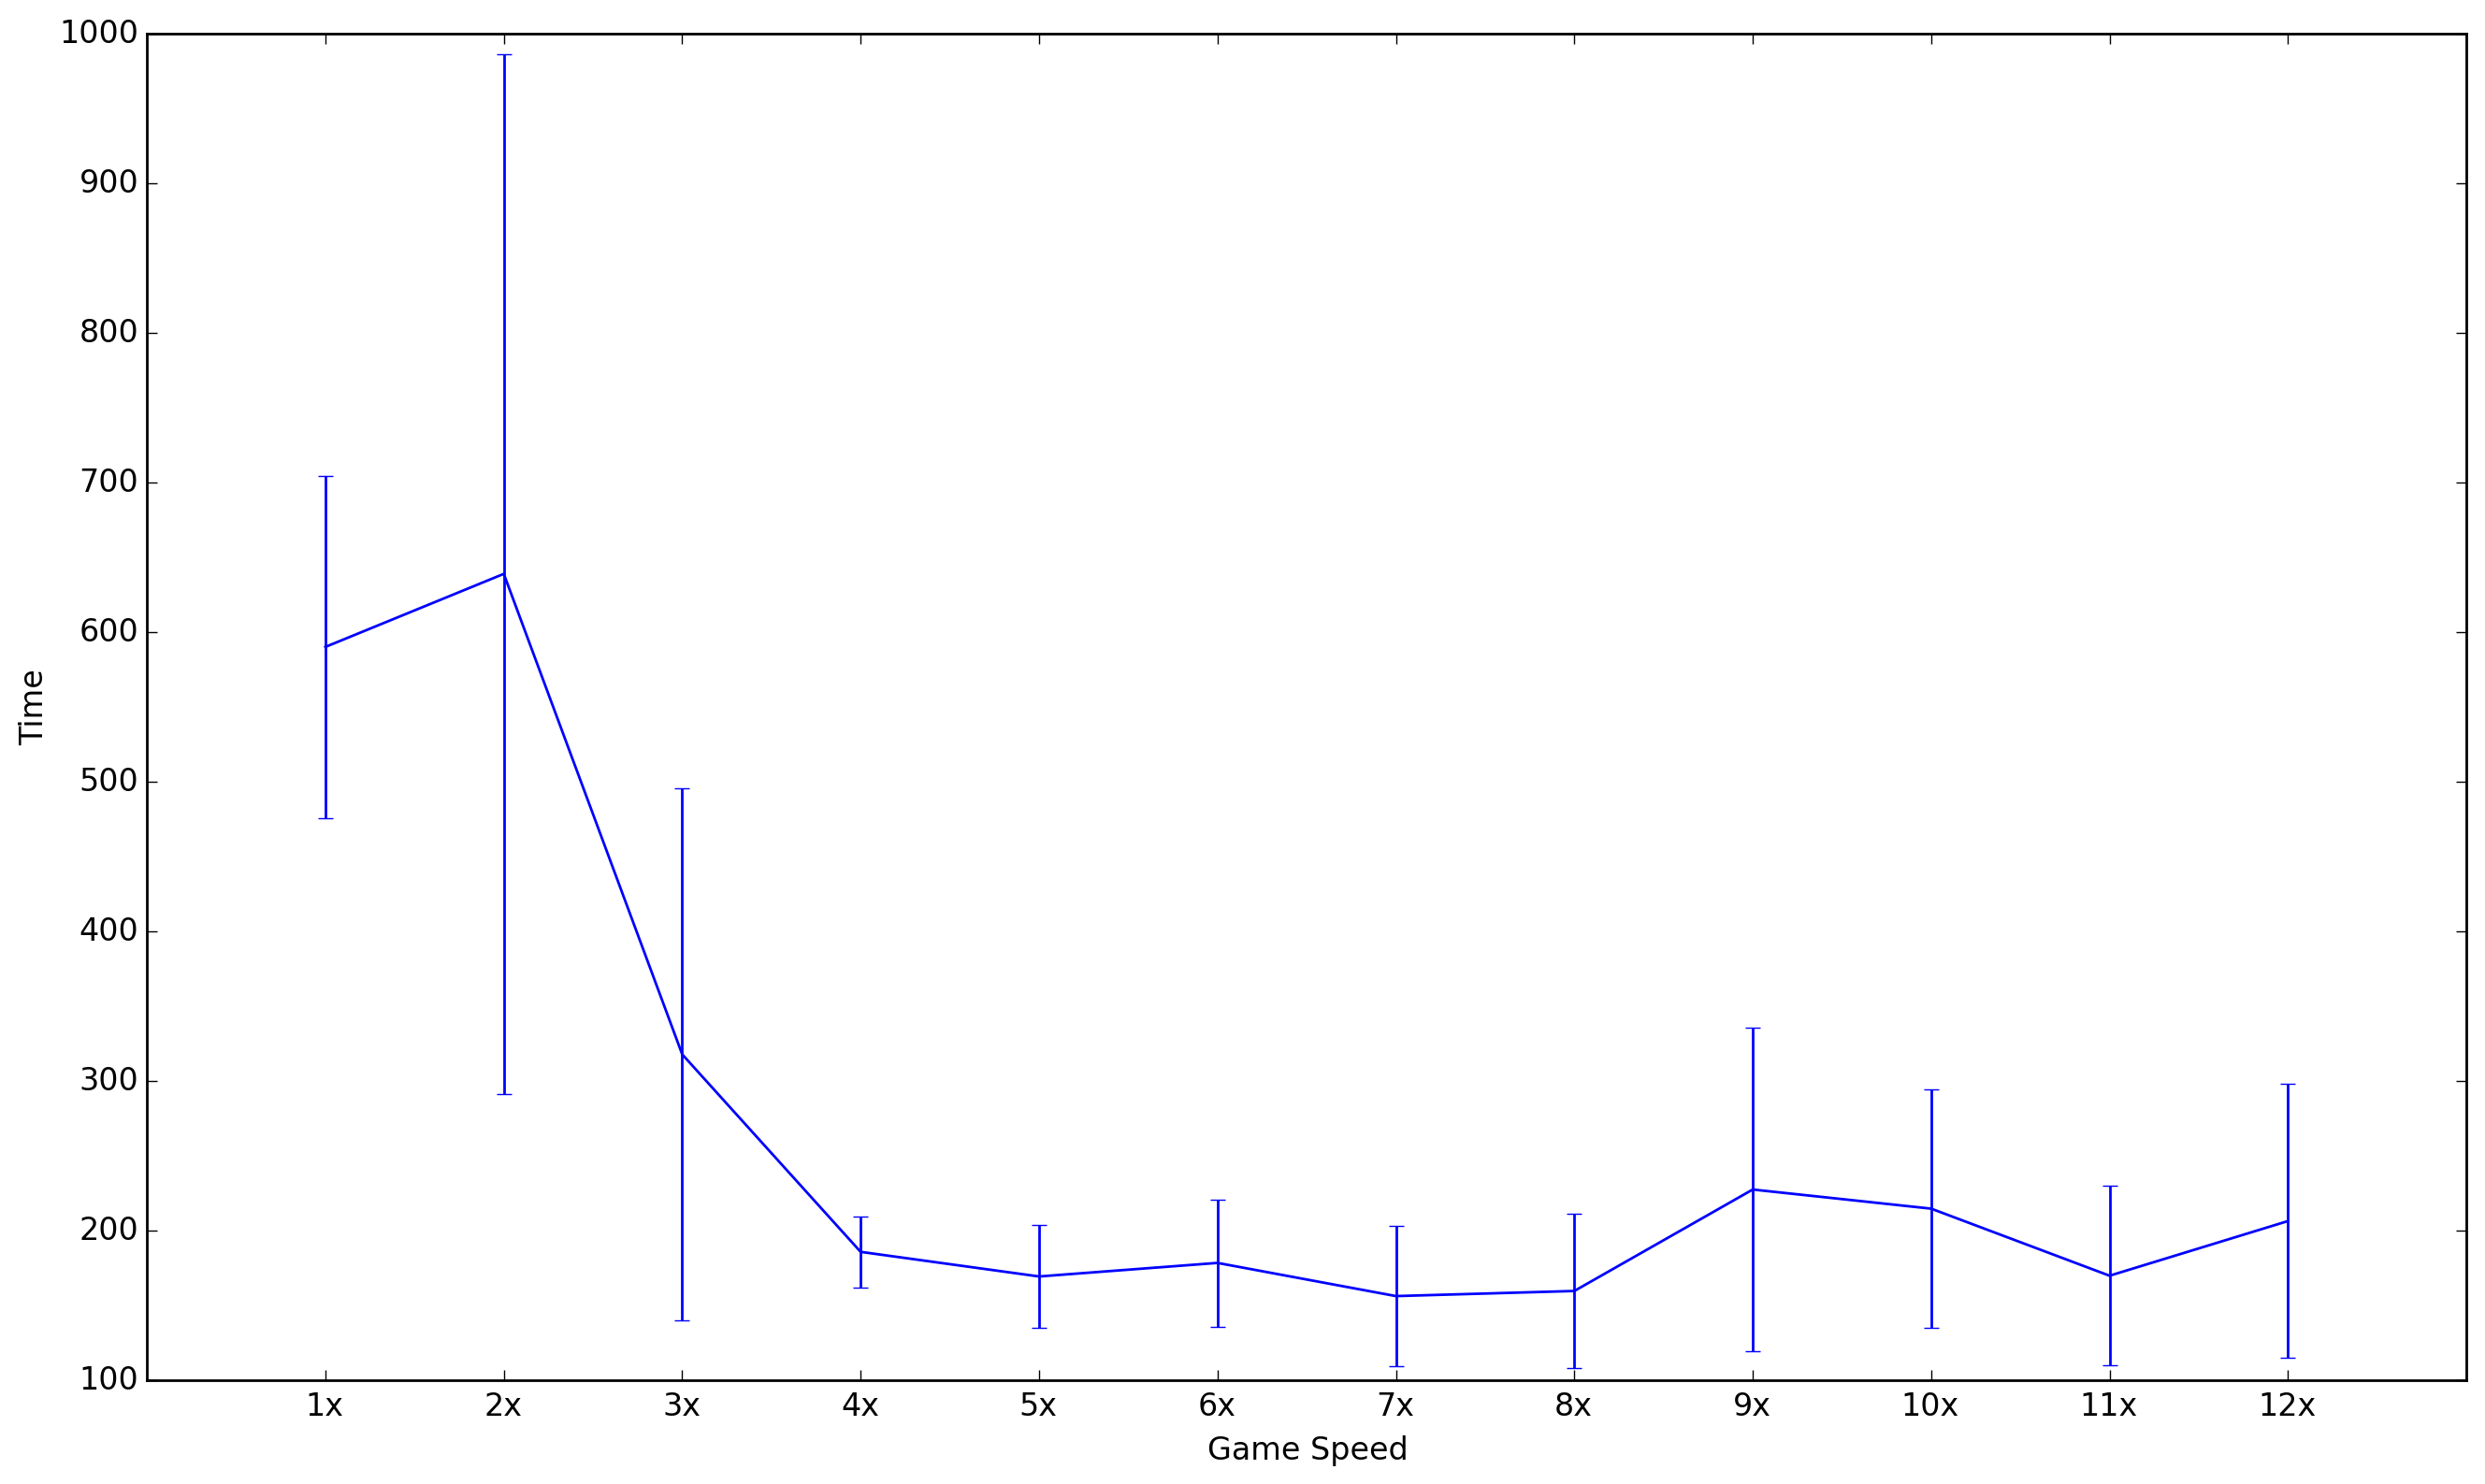
\includegraphics[width=1.0\textwidth]{time_speed_2}
\caption{Tempi delle simulazioni con la seconda coppia di armi}
\label{fig:time_speed_2}
\end{figure}

\begin{figure}[htp]
\centering
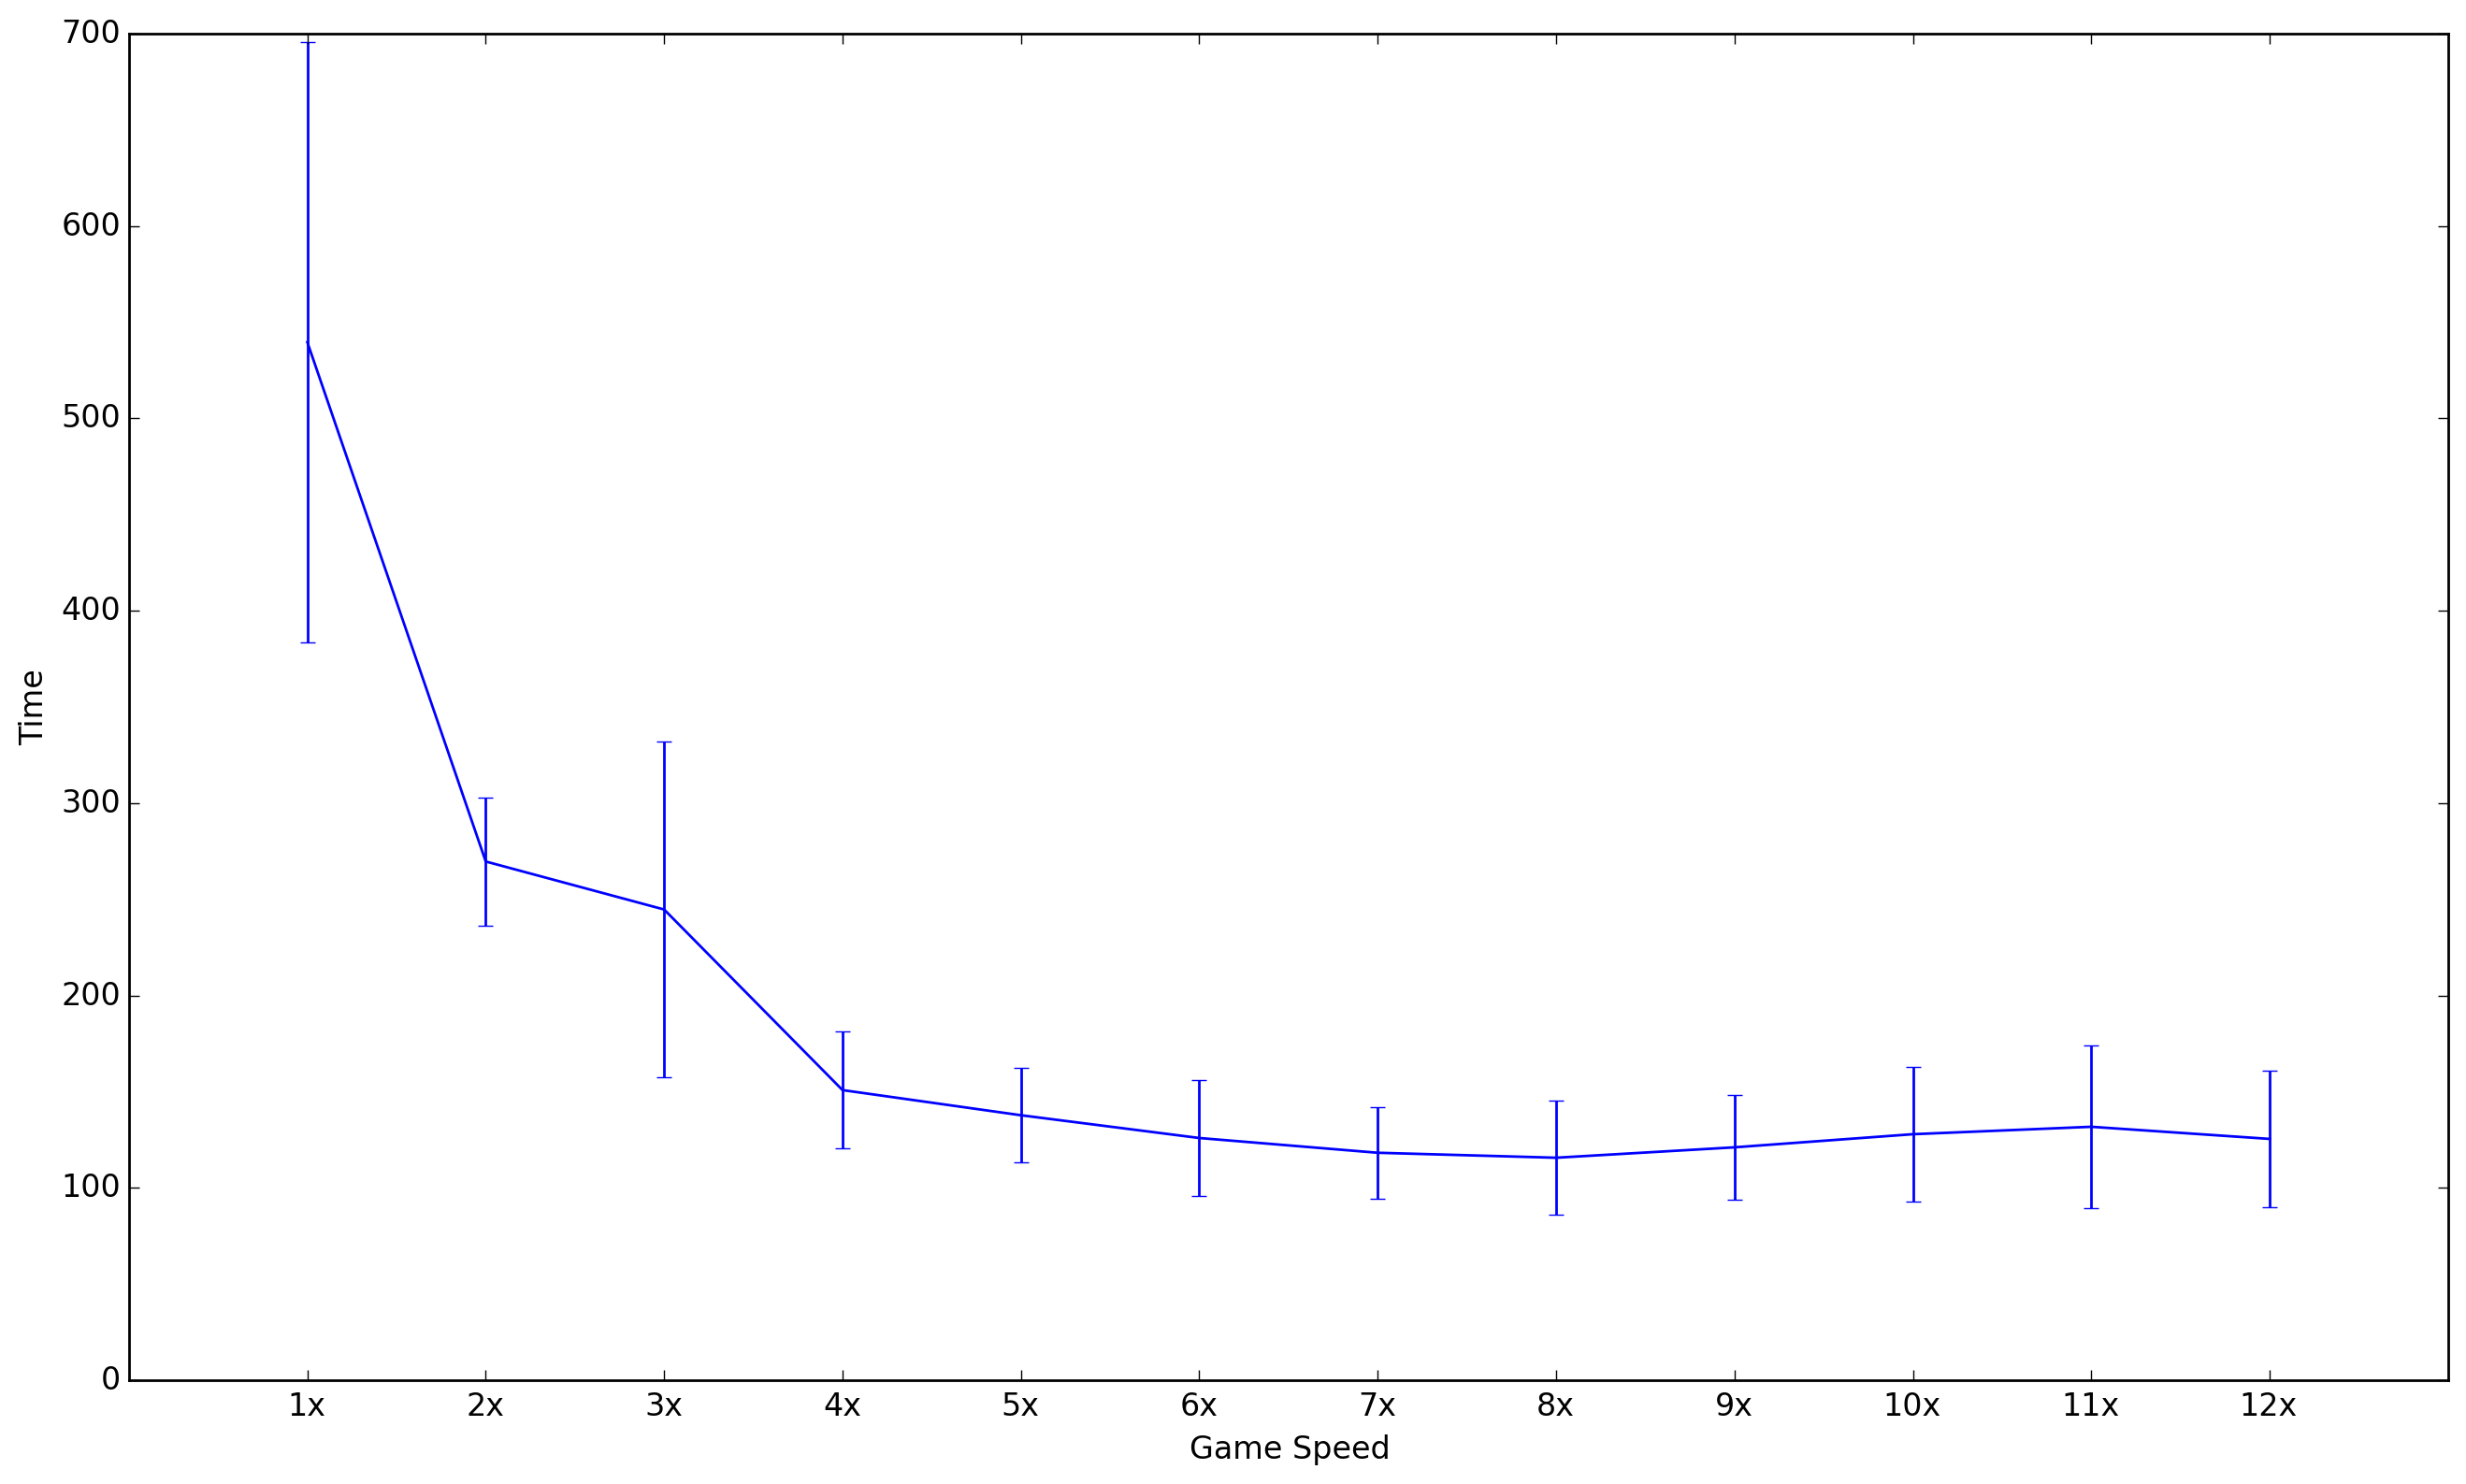
\includegraphics[width=1.0\textwidth]{time_speed_3}
\caption{Tempi delle simulazioni con la terza coppia di armi}
\label{fig:time_speed_3}
\end{figure}

I grafici  \ref{fig:time_speed_1}, \ref{fig:time_speed_2} e \ref{fig:time_speed_3} mostrano la media e la deviazione standard dei tempi ottenuti nelle 10 simulazioni per tutti gli incrementi di velocità compresi tra 1x (velocità normale) e 12x (velocità incrementata di 12 volte).
Dai grafici si nota un rapido decremento del tempo di simulazione fino alla velocità 4x e successivamente un decremento più contenuto fino alla velocità 8x, per poi ricominciare ad aumentare nei successivi incrementi.
Abbiamo quindi deciso di prendere come velocità ottimale l'incremento 8x. Nonostante la velocità sia stata incrementata di 8 volte rispetto al normale, il rapporto effettivo tra velocità maggiorata e velocità normale è solo di circa 3x: questo dimostra le considerazioni fatte precedentemente , in quanto è probabile che la logica che gestisce l'intelligenza artificiale venga chiamata con meno frequenza rispetto alle velocità più basse. Questo purtroppo non lo possiamo verificare in modo puntuale in quanto il codice sorgente dell'engine non è disponibile.

Una volta decisa la velocità di gioco, abbiamo verificato che il gioco si comportasse in modo corretto anche alle velocità maggiori. Infatti è possibile che a una velocità incrementata la logica dedicata all'intelligenza artificiale non si comporti più correttamente, perché non essendo stata progettata per funzionare a queste velocità, il suo comportamento potrebbe essere meno affidabile rispetto a una velocità normale. 
Per verificarne il comportamento, abbiamo raccolto le statistiche relative alle uccisioni ottenute dai bot rispetto alla velocità normale e alla velocità incrementata di 8 volte.

\begin{figure}[htp]
\centering
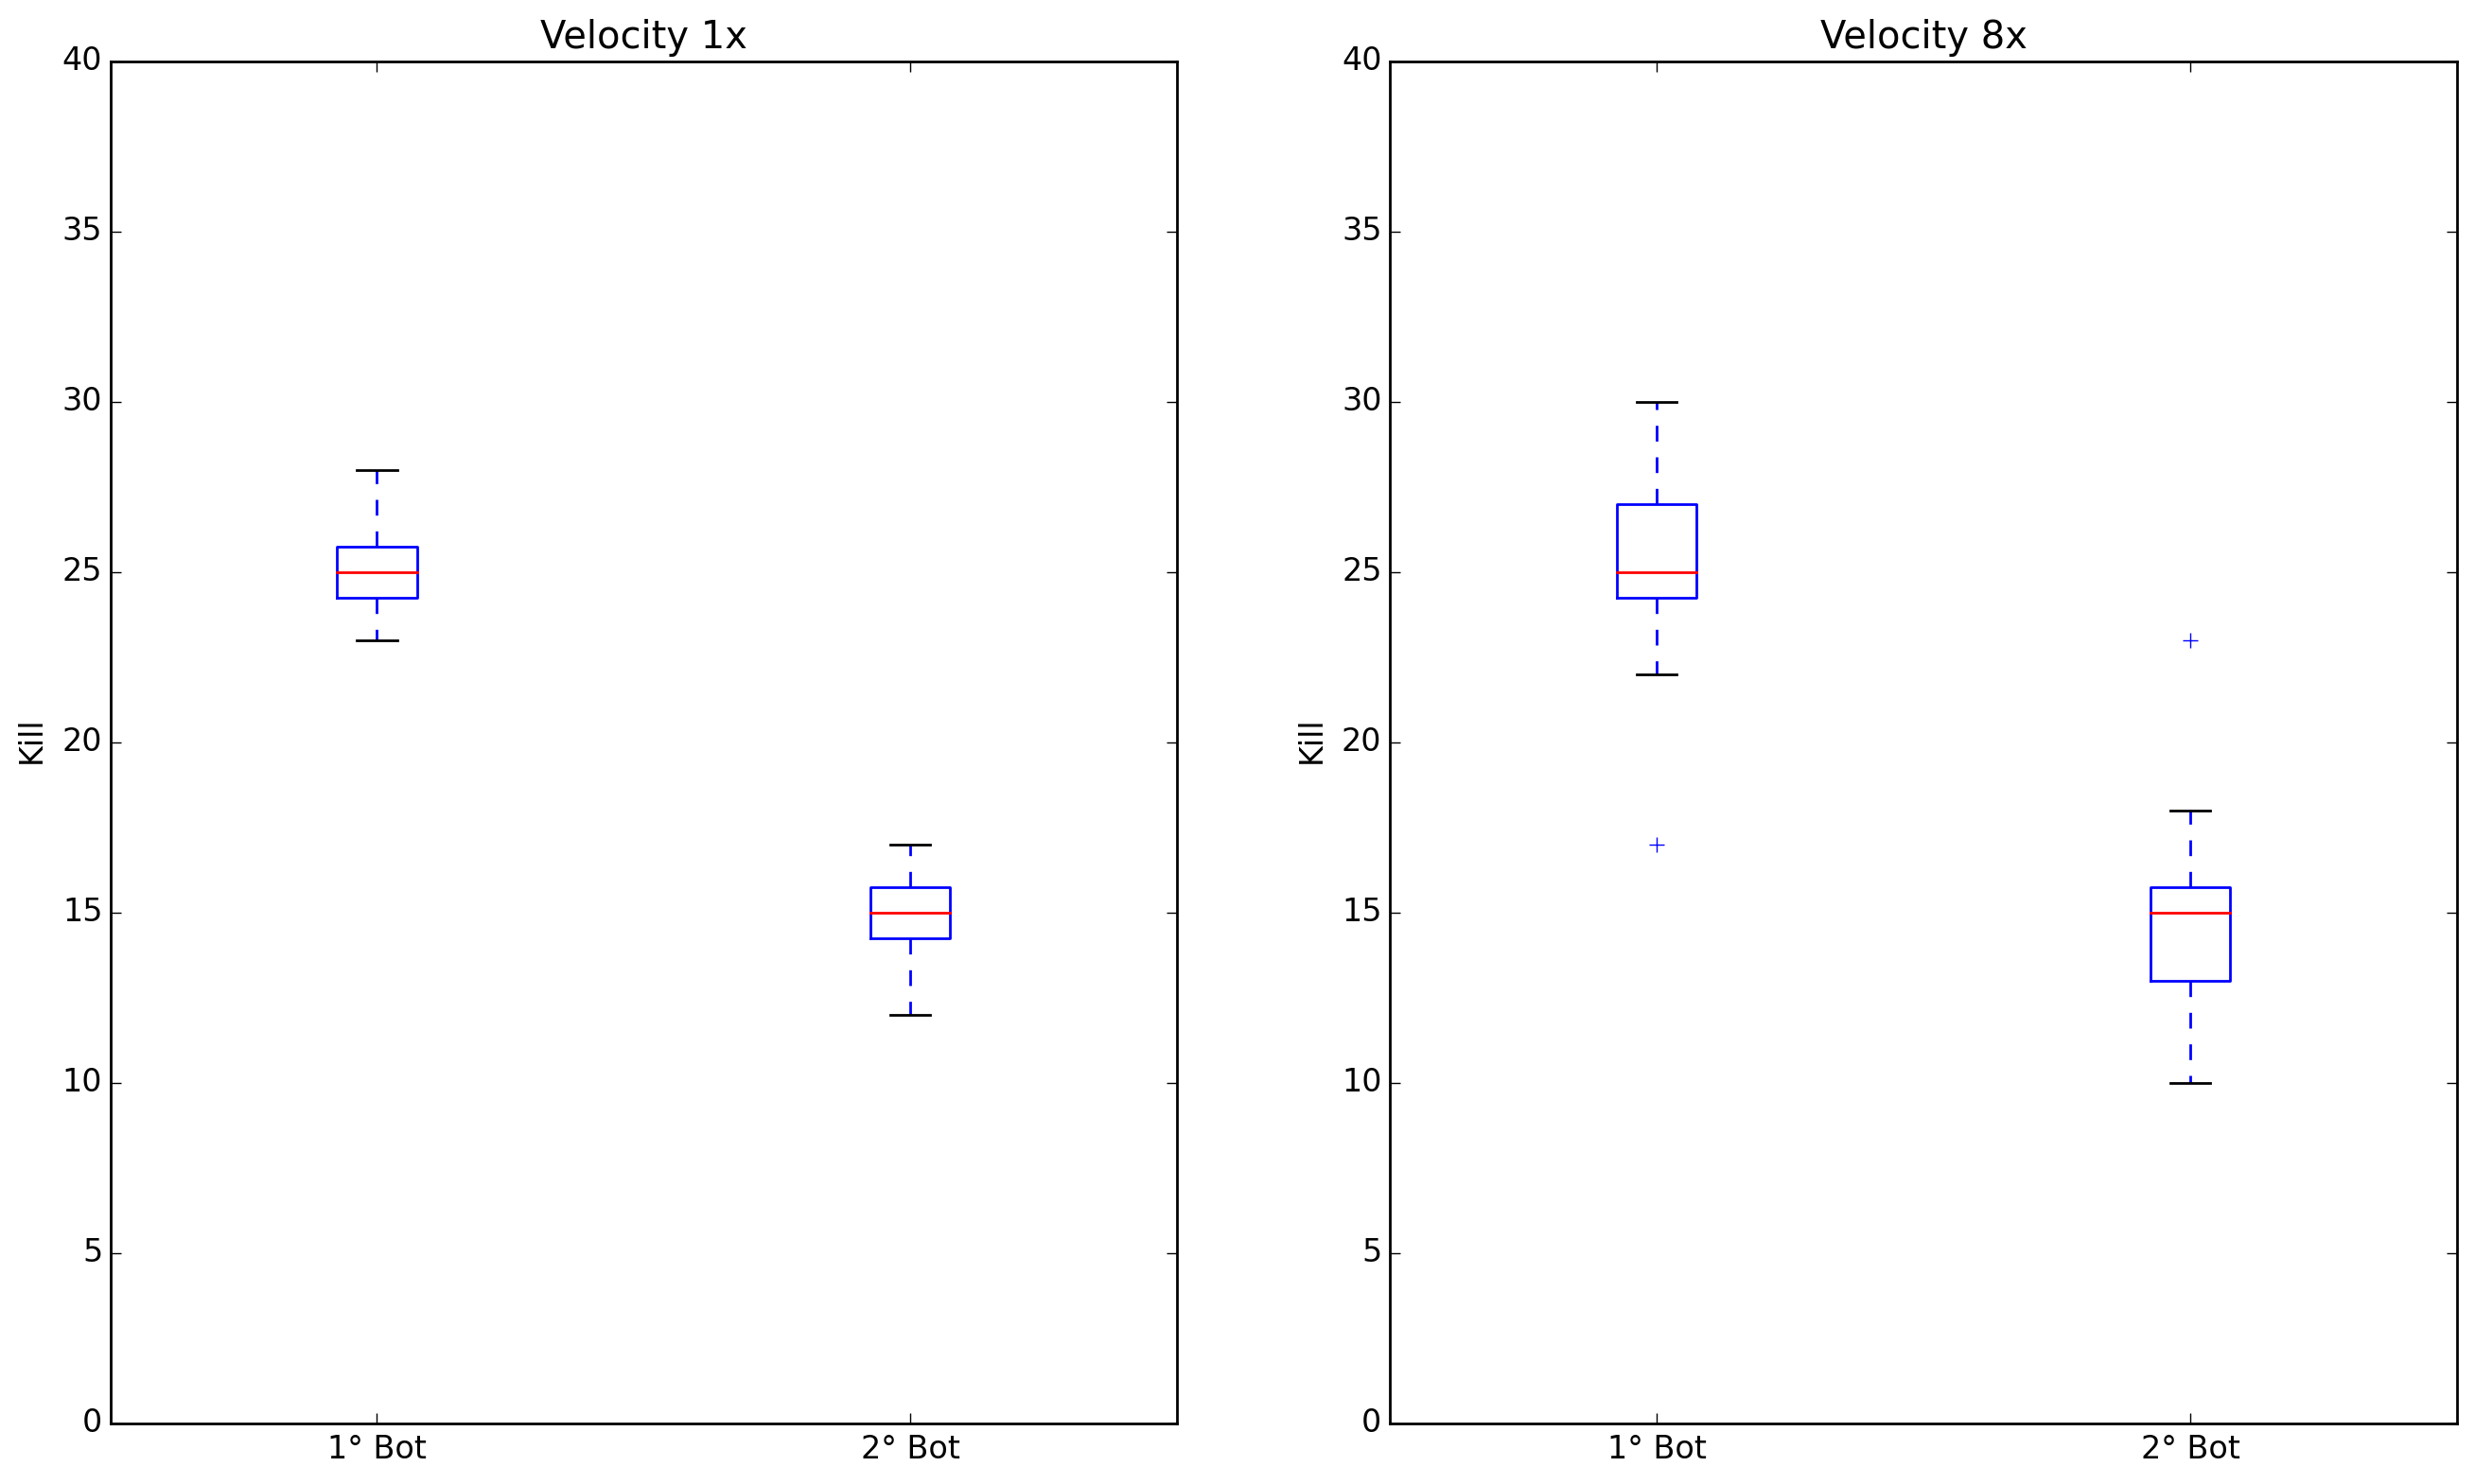
\includegraphics[width=1.0\textwidth]{1vs8_1}
\caption{Risultati delle uccisioni ottenute dai due bot con la prima coppia di armi}
\label{fig:kill_vs_speed_1}
\end{figure}

\begin{figure}[htp]
\centering
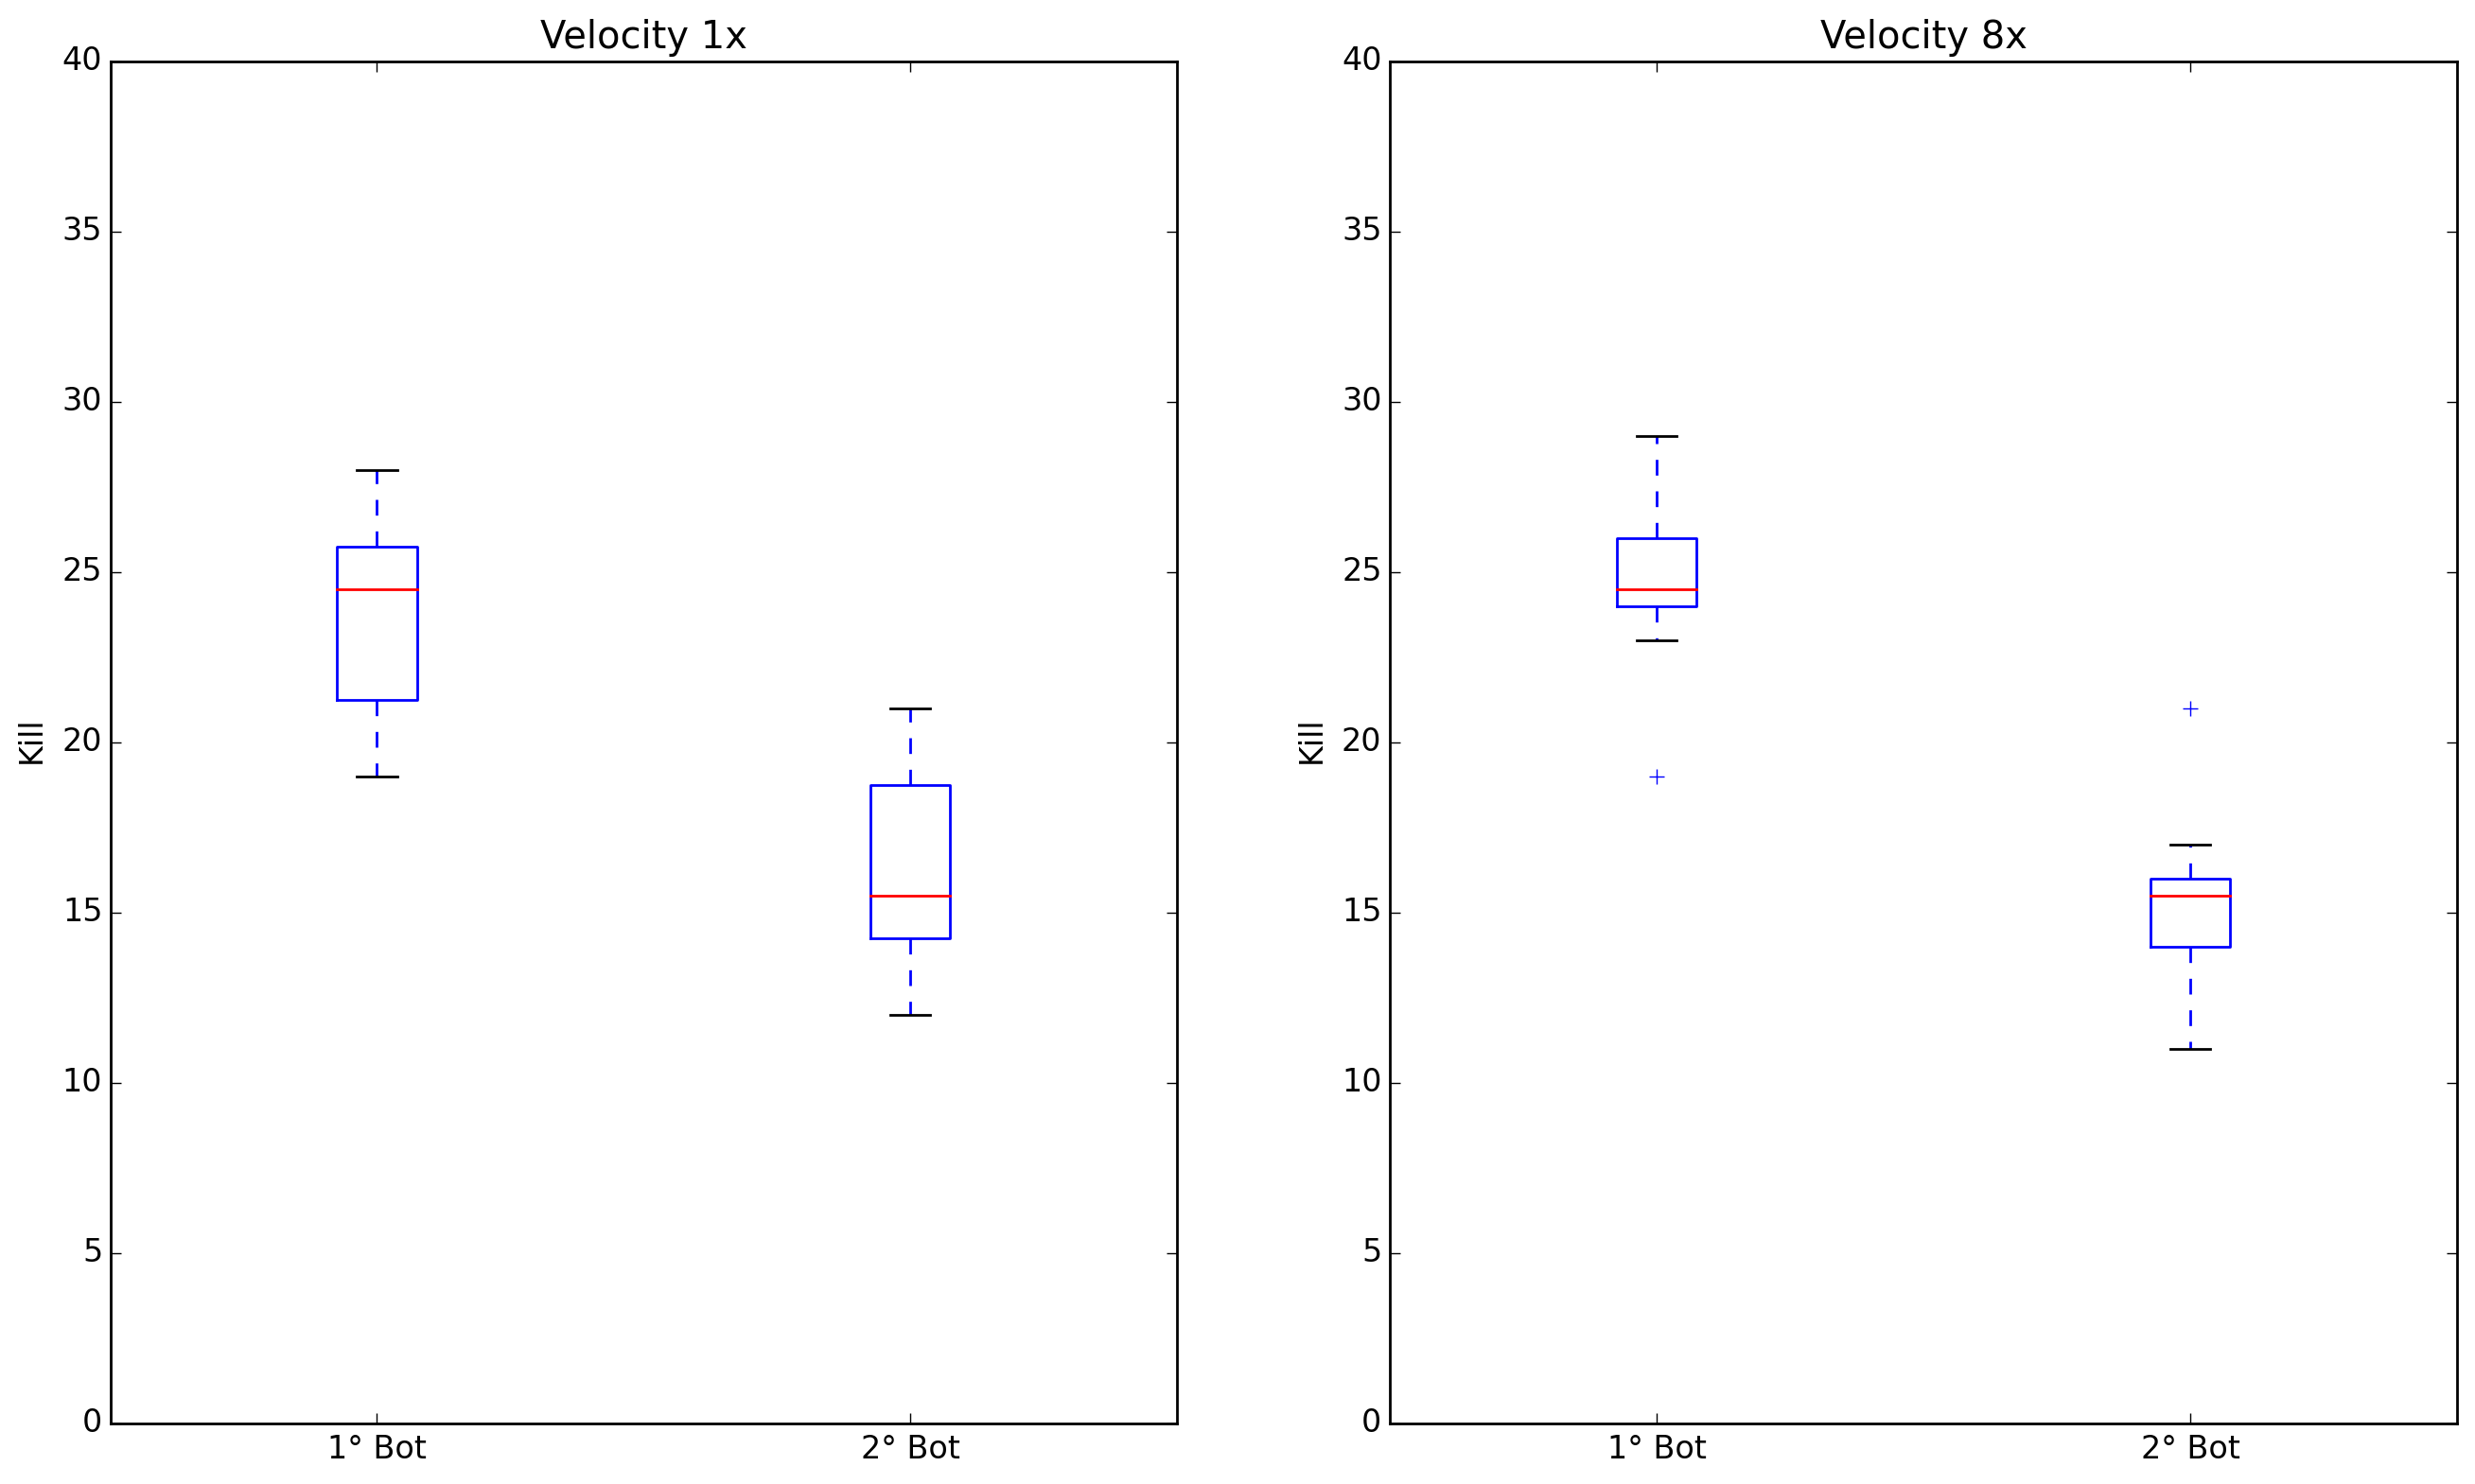
\includegraphics[width=1.0\textwidth]{1vs8_2}
\caption{Risultati delle uccisioni ottenute dai due bot con la seconda coppia di armi}
\label{fig:kill_vs_speed_2}
\end{figure}

\begin{figure}[htp]
\centering
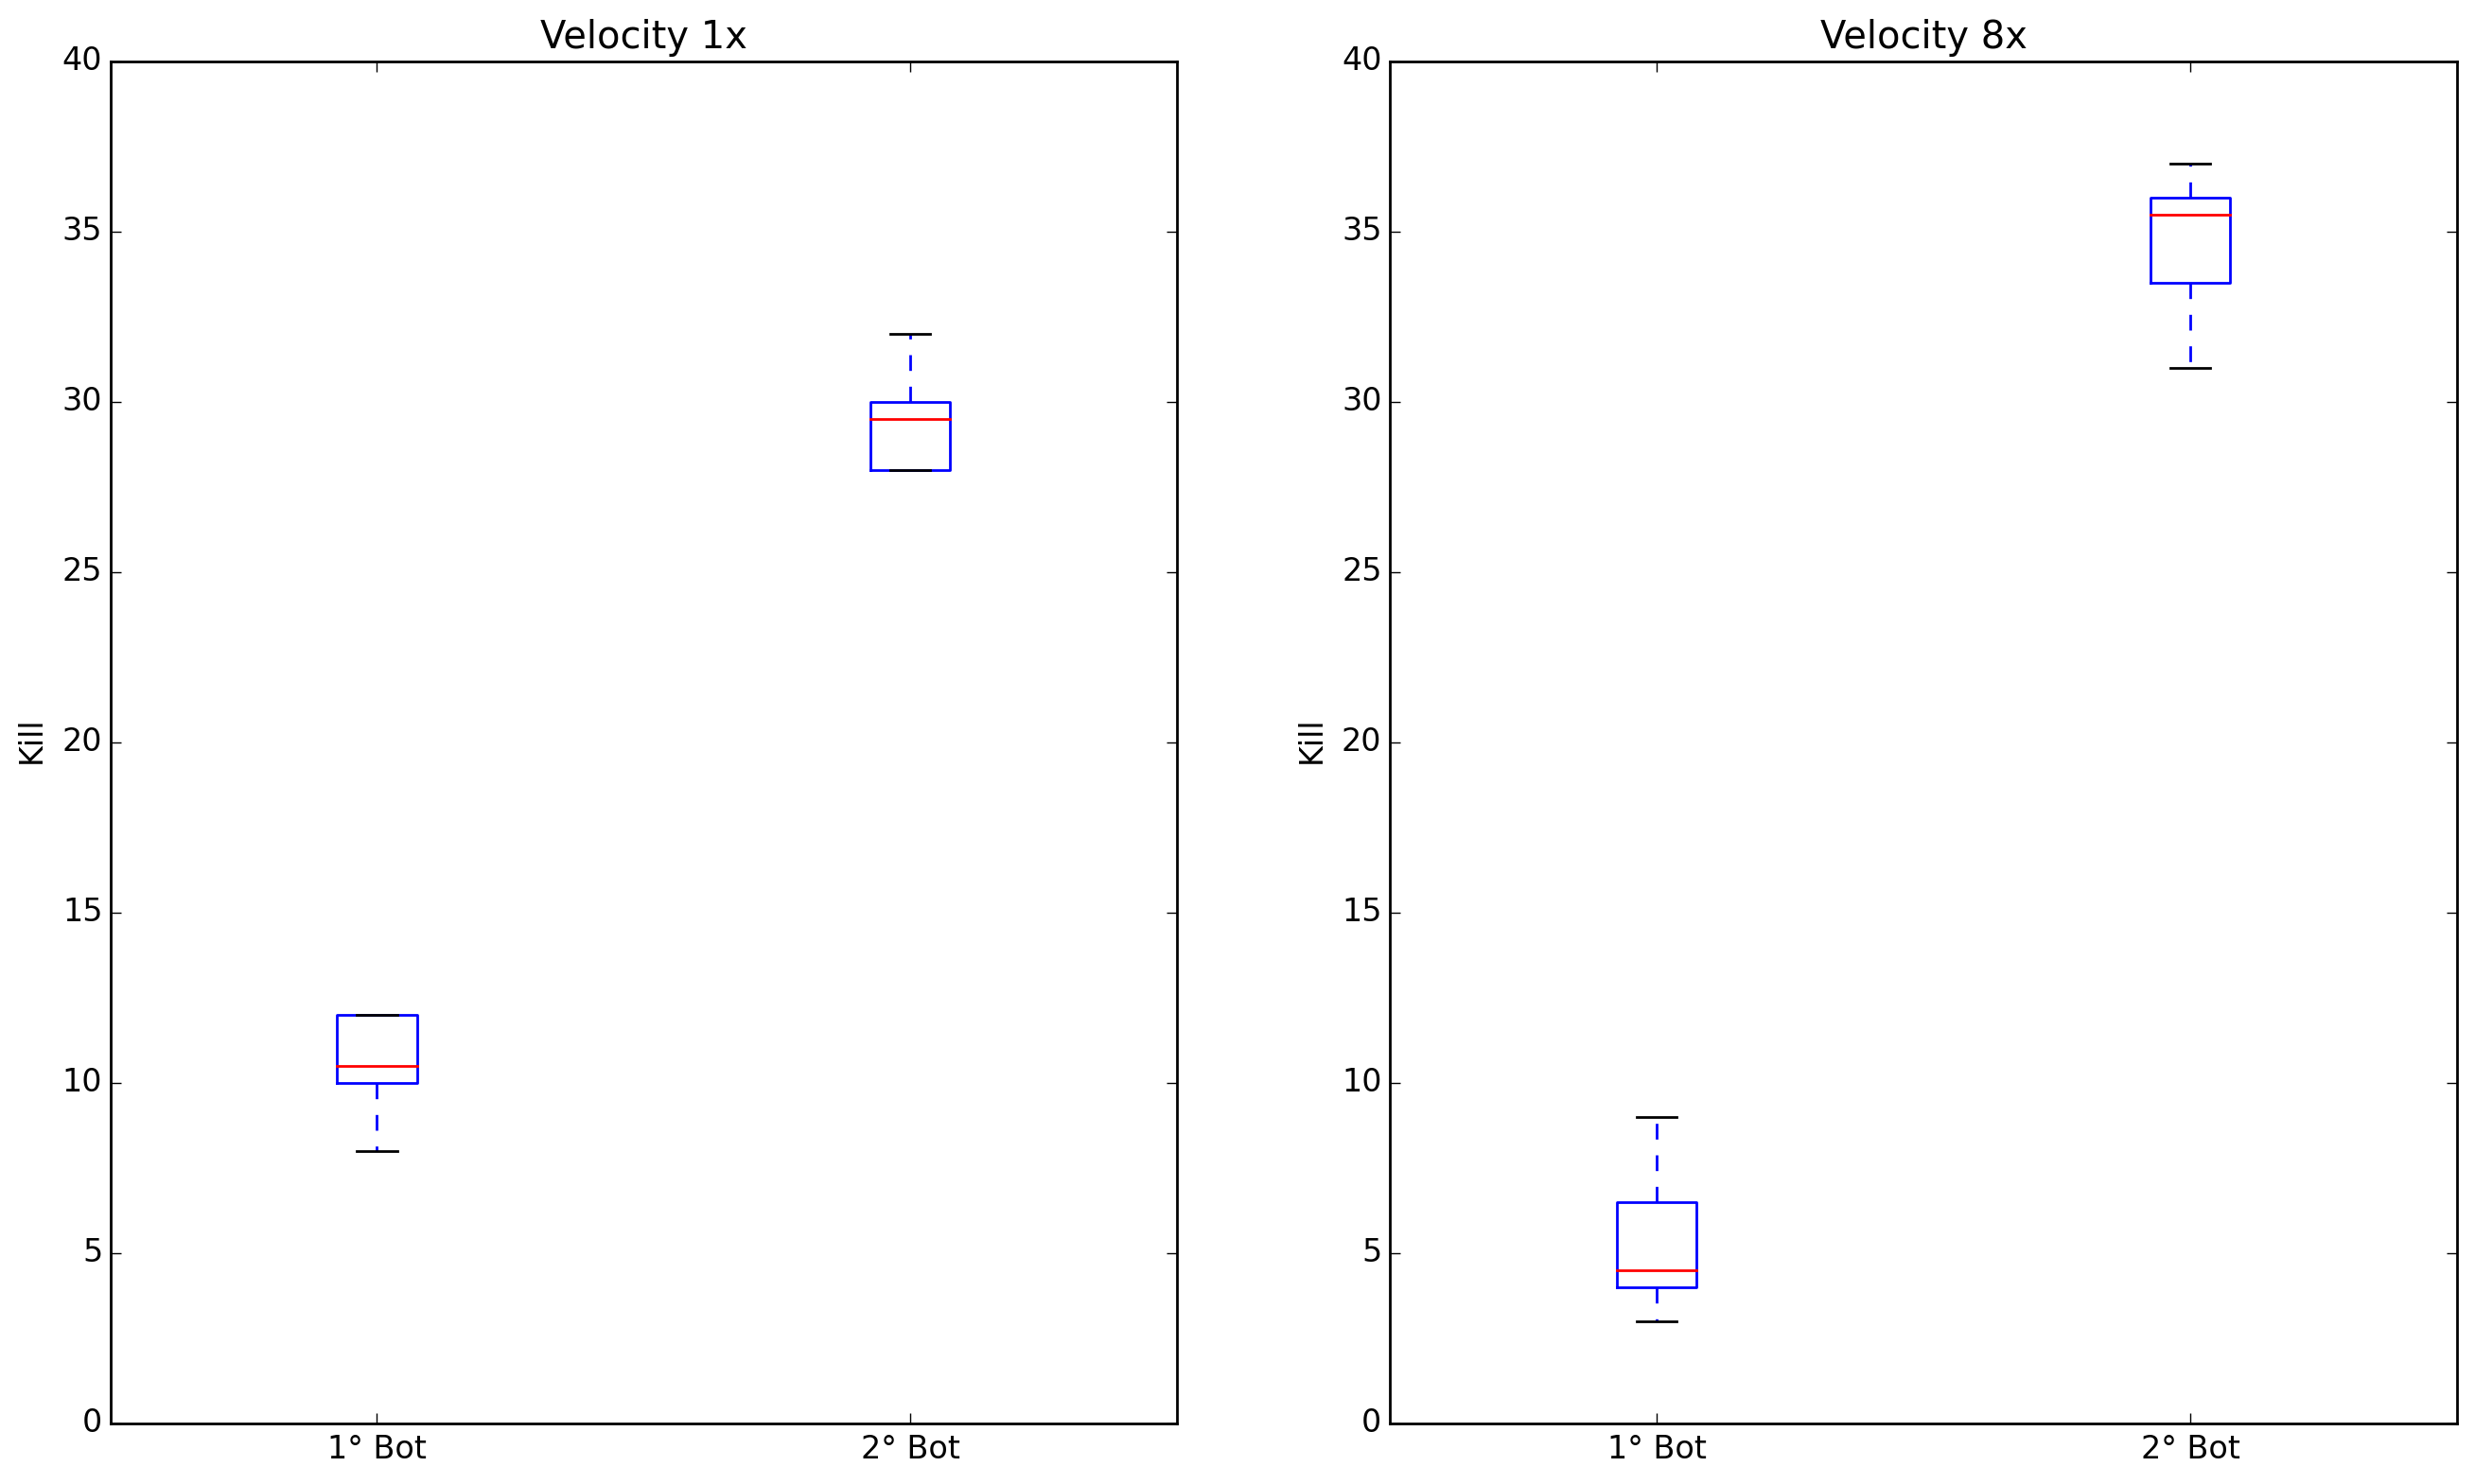
\includegraphics[width=1.0\textwidth]{1vs8_3}
\caption{Risultati delle uccisioni ottenute dai due bot con la terza coppia di armi}
\label{fig:kill_vs_speed_3}
\end{figure}

Le figure \ref{fig:kill_vs_speed_1}, \ref{fig:kill_vs_speed_2}, \ref{fig:kill_vs_speed_3} mostrano i \emph{boxplot} delle uccisioni ottenute dai due bot con le tre coppie di armi usate nei esperimenti precedenti, confrontando le due velocità scelte, cioè velocità normale (1x) e velocità incrementata (8x).
Si nota che abbiamo un comportamento molto simile nel caso le armi siano abbastanza equilibrate (\ref{fig:kill_vs_speed_1}), mentre abbiamo qualche leggera differenza in più con la terza coppia di armi (\ref{fig:kill_vs_speed_3}), dove risulta esserci un divario più accentuato nel caso della velocità 8x.

Dopo queste valutazioni abbiamo deciso che il miglior compromesso tra velocità ed errore è la velocità 8x, che ci consente di avere il tempo di simulazione più basso, a costo di un piccolo errore nel caso le armi non siano equilibrate, ma che diminuisce ulteriormente man mano che le armi diventano più bilanciate.

\subsubsection{Il Goal Score e il tempo limite di simulazione}
\label{sec:goal_score}
Una volta deciso la velocità più adatta per le simulazioni, abbiamo dovuto scegliere il \emph{goal score} da impostare per le simulazioni.
Il \emph{goal score} è il limite di uccisioni totali dei due bot che determina la fine della simulazione, a meno che la durata della partita superi il limite di tempo imposto per la partita.
Per decidere il \emph{goal score}, dobbiamo valutare quale sia un buon candidato che ci permetta di ottenere dei risultati affidabili nel minor tempo possibile. 
La durata della partita infatti dipende, oltre dalla velocità della simulazione, anche dal \emph{goal score}: se questo è troppo piccolo la simulazione potrebbe darci risultati poco affidabili, in quanto andrebbe a imporre un numero troppo esiguo di uccisioni per avere dei risultati affidabili in termini statistici, mentre se troppo grande, renderebbe troppo lunghe le simulazioni e considerando che dobbiamo eseguire all'incirca 500 simulazioni per ogni prova degli esperimenti, il tempo necessario per simulazione diventa un problema da considerare attentamente.
Quindi abbiamo eseguito dei test per verificare come si comportano le armi a seconda di come cambia il \emph{goal score}.
Dal momento che gli esiti della simulazione sono influenzati anche dal tipo di armi usate, abbiamo svolto la nostra analisi usando due diverse coppie di armi per ridurre tale dipendenza nei risultati ottenuti.
I test sono stati eseguiti con 4 diversi \emph{goal score}: 20, 40, 80 e 160. Per ogni coppia abbiamo eseguito 10 simulazioni.

\begin{figure}[htp]
\centering
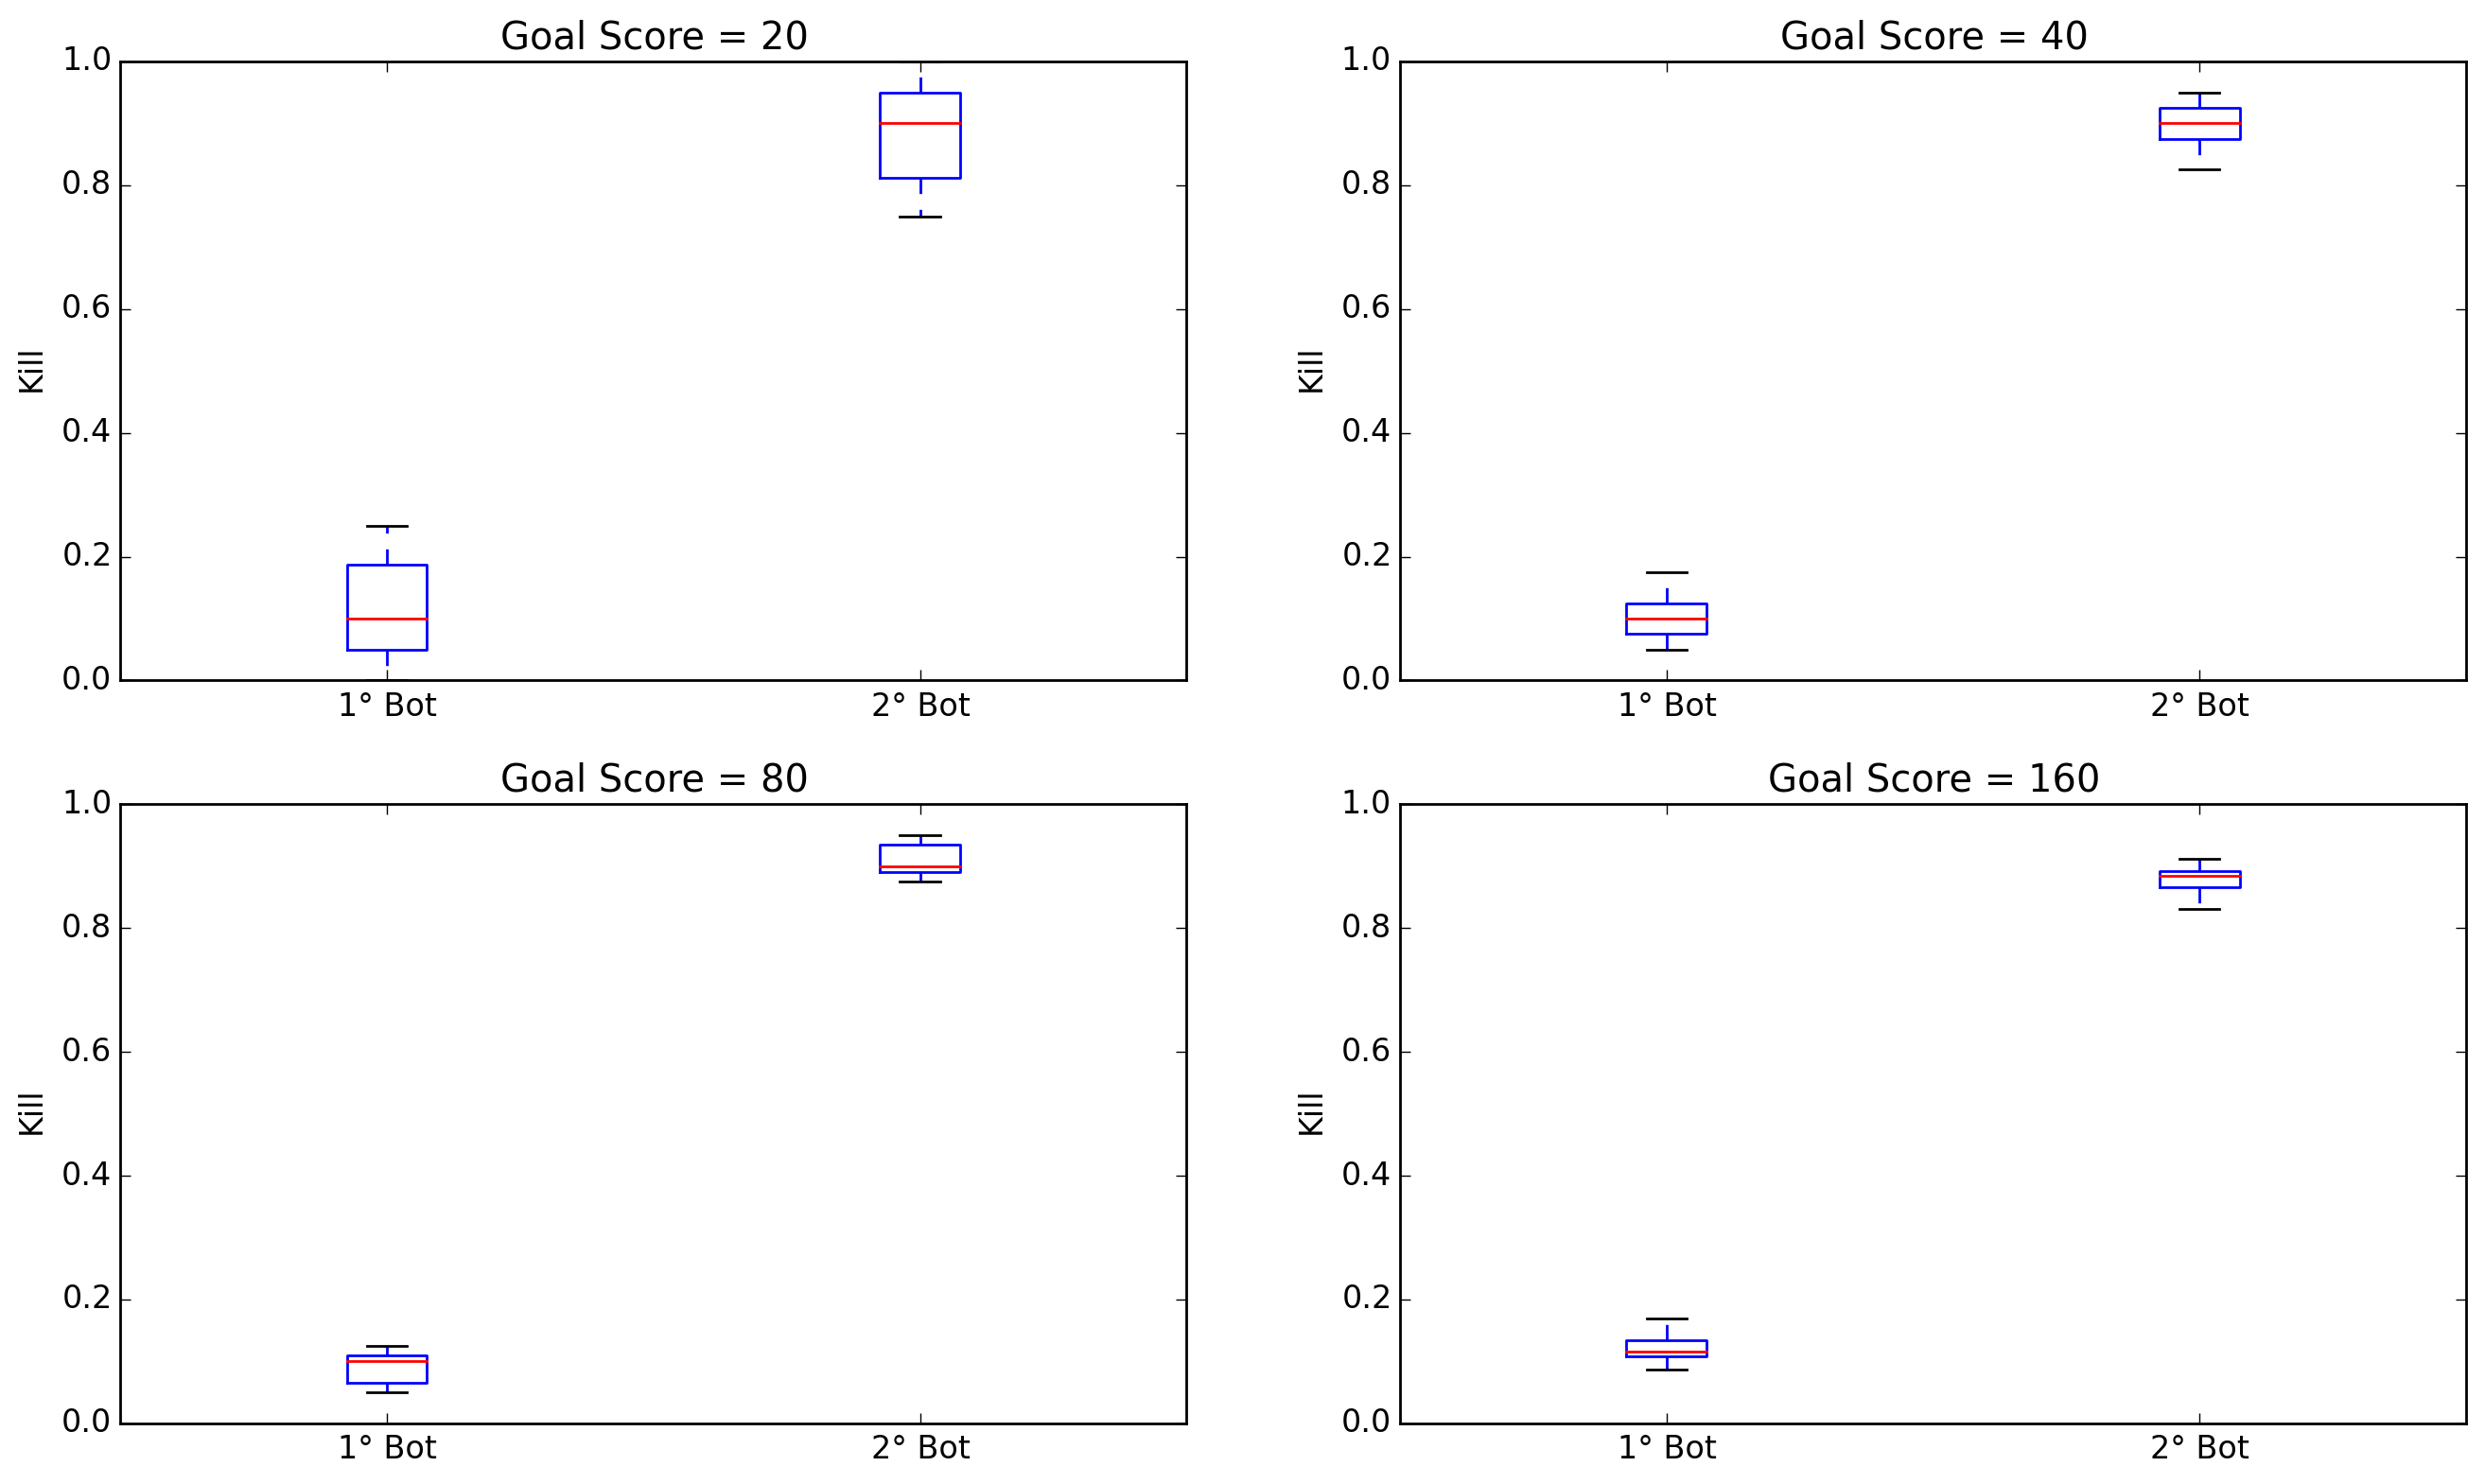
\includegraphics[width=1.0\textwidth]{kill_vs_gs_1}
\caption{\emph{boxplot} delle uccisioni dei due bot con la prima coppia di armi}
\label{fig:kill_vs_gs_1}
\end{figure}
\begin{figure}[htp]
\centering
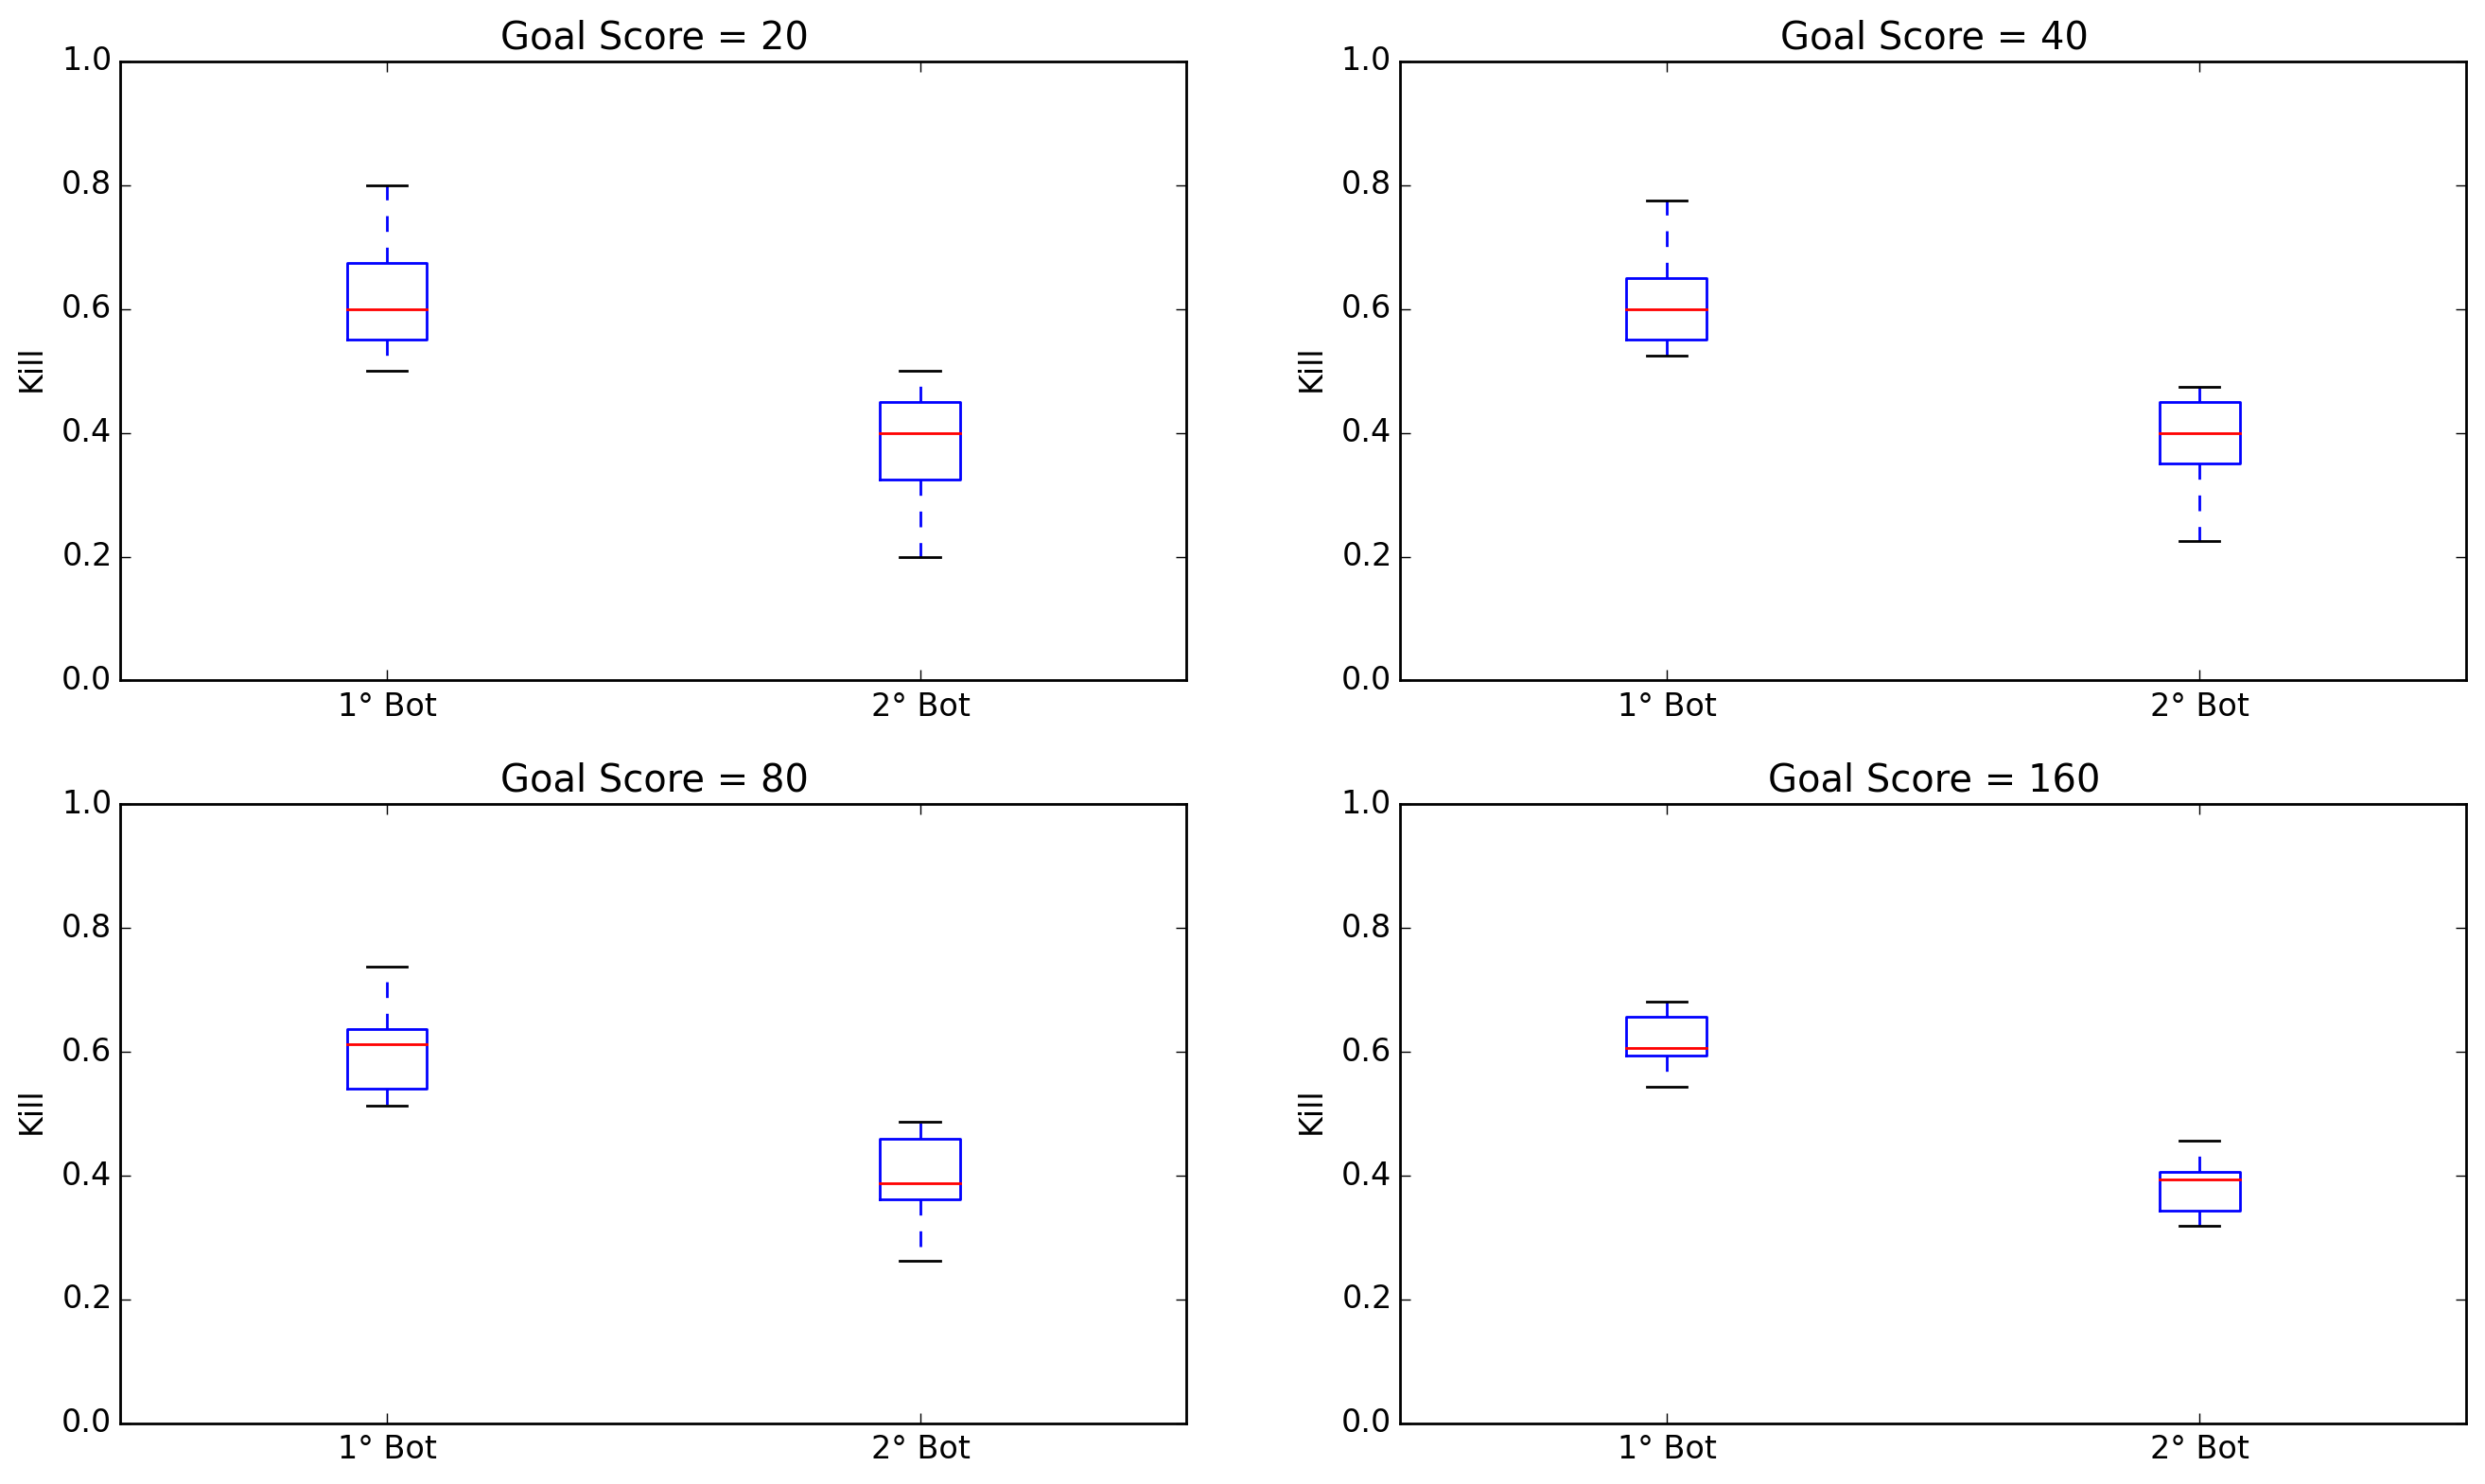
\includegraphics[width=1.0\textwidth]{kill_vs_gs_2}
\caption{\emph{boxplot} delle uccisioni dei due bot con la seconda coppia di armi}
\label{fig:kill_vs_gs_2}
\end{figure}

Le figure \ref{fig:kill_vs_gs_1} e \ref{fig:kill_vs_gs_2} mostrano i risultati con due coppie di armi: per ogni \emph{goal score} mostriamo i \emph{boxplot} delle uccisioni ottenute con le due armi. I risultati sono stati normalizzati a 1, in modo da ottenerne una migliore visualizzazione.
I grafici mostrano come la precisione della simulazione aumenta gradualmente con l'aumentare del \emph{goal score}.
Abbiamo deciso che per le nostre simulazioni il \emph{goal score} ottimale è 20, in quanto è abbastanza affidabile rispetto ai \emph{goal score} più alti, e il tempo di esecuzione medio è intorno ai 100 secondi, un tempo accettabile rispetto al numero di simulazioni richieste dal nostro lavoro.

Una volta deciso il \emph{goal score}, abbiamo dovuto valutare come impostare il limite di tempo delle simulazioni. Infatti nel caso due armi non siano utilizzabili dai bot (un certa combinazione di parametri potrebbe rendere l'arma inutilizzabile) la partita potrebbe non terminare mai, in quanto i due bot non riuscirebbero a ottenere alcuna uccisione. Inoltre può capitare che in alcuni rari casi il comportamento dell'intelligenza artificiale sia particolarmente difettosa, in quanto a una velocità maggiorata è possibile constatare dei casi in cui il comportamento dei bot non sia corretto, il che determina una durata più lunga e dei risultati errati.
Per affrontare questi problemi abbiamo introdotto nelle simulazioni un tempo limite per partita.

Sulla base dei tempi medi ottenuti dalle due coppie di armi prese in considerazione nei test precedenti, con una configurazione con velocità incrementata di 8 volte e con un\emph{goal score} pari a 20, abbiamo constatato che il tempo medio è di 100 secondi, e quindi abbiamo optato per un tempo limite di 150 secondi a velocità incrementata, che a velocità normale corrispondono a 1200 secondi.
Questo lascia un certo margine che permette a due armi di ottenere il numero di uccisioni richiesto e permette di avere dei tempi massimi di simulazione accettabili per i fini dei nostri esperimenti.

\section{Sommario}
In questo capitolo abbiamo introdotto i nostri obiettivi per questo lavoro e l'ambiente simulativo degli esperimenti.
Nella Sezione 3.1 introduciamo nel dettaglio quali sono i nostri obiettivi.
Nella Sezione 3.2 descriviamo il gioco utilizzato per le simulazioni, Unreal Tournament III.
Infine nella Sezione 3.3 descriviamo l'ambiente simulativo costruito per i nostri esperimenti, e spieghiamo come abbiamo deciso la velocità, il goal score e tempo limite delle simulazioni.

\chapter{Generazione libera di armi bilanciate} 
Per esplorare le potenzialità creative dell'algoritmo genetico applicato allo spazio delle armi, abbiamo valutato come primo esperimento la generazione di armi equilibrate senza nessun vincolo aggiuntivo.
Lo scenario applicativo di questo esperimento è quello di realizzare uno strumento applicativo per i game designer che permetta di esplorare lo spazio delle armi bilanciate, e quindi valutare le capacità creative dell'algoritmo genetico.
Per questo motivo abbiamo deciso di utilizzare una algoritmo genetico a singolo obiettivo, il cui unico scopo sia generare coppie di armi bilanciate. 
Questo ci permette di esplorare lo spazio delle armi bilanciate e valutare quali caratteristiche debbono avere delle coppie di armi per risultare equilibrate.
Andremo quindi a descrivere il design sperimentale utilizzato per questo esperimento.
Successivamente descriviamo i risultati ottenuti nelle 10 prove effettuate dell'esperimento.
Infine andiamo a effettuare una validazione dei risultati ottenuti, rivalutando con una simulazione più precisa le coppie di armi ottenute nelle 10 prove dell'esperimento.

\section{Design Sperimentale}
\label{sec:entropy}
Ora andremo a descrivere l'implementazione dell'algoritmo genetico e i parametri scelti per la l'esperimento; successivamente descriveremo la funzione di fitness scelta per formalizzare il concetto di bilanciamento in una coppia di armi.

\subsection{Algoritmo e Parametri Sperimentali}
L'algoritmo utilizzato in questo esperimento è un algoritmo genetico a singolo obiettivo, dove l'obiettivo è la massimizzazione del bilanciamento delle armi generate.
Gli operatori genetici scelti per questo esperimento sono i seguenti:  per il crossover abbiamo scelto il \emph{simulated binary crossover} con probabilità 0.6; per la mutazione abbiamo scelto la \emph{simulated binary mutation} con probabilità 0.05; e infine come selezione abbiamo scelto la \emph{tournament selection} a tre individui.
La \emph{rappresentazione} degli individui consiste in un vettore di 20 parametri: ogni individuo consta di due armi, in particolare i primi dieci rappresentano i parametri della prima arma, e gli ultimi dieci sono i parametri della seconda arma.
Ogni parametro rappresenta una caratteristica dell'arma, come descritto nella Sezione~\ref{sec:setting}, quindi stiamo utilizzando un \emph{encoding} \emph{diretto}.
Dopo aver effettuato alcuni test, abbiamo constatato che per ottenere dei risultati soddisfacenti dal punto di vista della fitness il numero di generazioni ottimale fosse 50 con una popolazione di individui pari a 100.
Per l'implementazione dell'algoritmo abbiamo utilizzato una libreria {P}ython,  DEAP\cite{deap:article}, e abbiamo sviluppato un'architettura client-server, dove lato client l'algoritmo genetico testa le armi generate inviando i parametri al server, il quale lancia una simulazione nel gioco \emph{Unreal Tournament III} (come abbiamo descritto nella Sezione 3.3). 
La simulazione avviene in una mappa di piccole dimensioni, \emph{DM-Biohazard}, scelta tra quelle disponibili in UT3, e nella modalità \emph{Deathmatch}. La configurazione della partita è la seguente: ai bot viene assegnata una skill pari a 7 (cioè il massimo), un limite di uccisioni totali (\emph{goal score}) pari a 20 e un tempo limite di 1200 secondi.
Quindi una volta inviati i parametri delle armi al server, una delle due armi vengono assegnate ai bot, e viene lanciata la simulazione.
Una volta conclusa la simulazione il server invia i risultati al client, il quale elabora i dati ricevuti e li utilizza per calcolare la fitness delle armi.
Questo procedimento avviene per testare ogni coppia di armi generata dall'algoritmo evolutivo.
La durata media per completare un singolo esperimento si è attestata sulle 9 ore.

\subsection{Funzione di Fitness}
\label{subsec:fitness}

Per calcolare la fitness delle armi generate abbiamo considerato l'utilizzo di tre funzioni, le quali vanno a valutare tre diversi aspetti delle armi.
La prima funzione formalizza il concetto di equilibrio, cioè l'obiettivo principale di questo esperimento.
Questa funzione valuta l'entropia delle due armi:
\begin{equation}
f_e = - \sum_i u_i/T_u*log_2(u_i/T_u)
\end{equation}
dove $u_i$ sono le uccisioni ottenute dall'$i$-esimo bot, $T_u$ è la somma delle uccisioni totali ottenute dai due bot.
L'entropia ha un massimo pari a uno quando le armi sono perfettamente equilibrate, cioè hanno $u_1 = u_2$, e diminuisce man mano che le uccisioni ottenute dalle due armi divergono.
La seconda e la terza funzione invece valutano due aspetti secondari che abbiamo inserito per aiutare l'algoritmo genetico scegliere armi che abbiano dei requisiti di funzionalità fondamentali per ottenere dei risultati di buona qualità.
In particolare la seconda funzione valuta se le due armi hanno ottenuto un numero di uccisioni totali entro il tempo limite imposto alla simulazione. In questo modo andiamo a limitare la variabilità dei risultati introdotta da una valutazione parziale delle uccisioni ottenute dalle armi, cioè se le armi non ottengono abbastanza uccisioni nel tempo limite, la valutazione del loro bilanciamento è imprecisa in quanto avviene prima che le due armi siano riuscite ottenere un numero di uccisioni sufficiente.
Dal momento che abbiamo interesse a generare delle armi \emph{interessanti} e che due armi molto lente nel provocare danno all'avversario vengono considerate di poco interesse per i nostri scopi, abbiamo deciso di premiare le armi più efficienti nell'ottenere il numero di uccisioni desiderato nel tempo limite.
La funzione è la seguente:
\begin{equation}
f_g =  \frac{T_u}{G}
\end{equation}
dove $T_u$ è la somma delle uccisioni totali ottenute dai due bot, mentre $G$ è il \emph{goal score}. Quando le due armi ottengono entro il tempo limite un numero di uccisioni pari a \emph{goal score} abbiamo $f_g$ pari a uno, mentre diminuisce fino a minimo di zero nel caso contrario.
La terza funzione va a valutare il numero di suicidi provocati dalle armi generate. Alcuni parametri delle armi, per esempio il raggio esplosivo dei proiettili, possono provocare dei suicidi nei bot che le usano. Questo è un comportamento delle armi che abbiamo deciso di penalizzare, in quanto un'arma di questo tipo è di poco interesse per i nostri fini e inoltre incrementa l'errore sulla valutazione delle armi, in quanto introduce un fattore aleatorio sul numero di uccisioni ottenute dalle armi.
La funzione è la seguente:
\begin{equation}
f_s =  0.9^{T_s}
\end{equation}
dove $T_s$ è il numero di suicidi totali ottenute dai due bot. Questa funzione ha un massimo pari a uno quando il numero di suicidi totali è pari a 0, e diminuisce man mano che il numero di suicidi aumenta.
Queste due funzioni, $f_s$ e $f_g$, contribuiscono a incrementare la fitness media della popolazione nella fasi iniziali di ricerca dell'algoritmo. Una volta che popolazione consta di individui che riescono a soddisfare questi due requisiti da noi imposti con queste due funzioni, il loro valore non andrà più a influenzare la fitness,  in quanto avremo armi che riescono sempre a raggiungere un numero di uccisioni pari a $G$ ($f_g = 1$) e non provocano suicidi  ($f_s = 1$).
Quindi la funzione di fitness è la somma di queste tre funzioni:
\begin{equation}
fitness = f_e + f_g + f_s
\end{equation}
La funzione di fitness ha come massimo 3, cioè quando la coppia di armi risulta equilibrata, con un numero di uccisioni totali ottenute nella simulazione pari a \emph{goal score} e con una somma pari a zero di suicidi, mentre ha come minimo 0,
cioè nel caso in cui tutte e tre le funzioni diano contributo pari a 0 nel calcolo della fitness totale.

\section{Risultati}

Ora andremo a descrivere in dettaglio i risultati ottenuti con gli esperimenti effettuati con la configurazione appena descritta.
Per valutare in media le prestazioni dell'algoritmo genetico, l'esperimento è stato ripetuto 10 volte. Per ogni esperimento abbiamo raccolto la fitness della popolazione per ogni generazione e gli individui delle popolazioni finali prodotte dalle 10 prove dell'esperimento effettuate.
Nell'analisi delle prestazioni andremo a descrivere come si è comportato l'algoritmo a livello di fitness per ogni generazione delle 10 prove effettuate.
Successivamente andiamo ad analizzare le caratteristiche emergenti delle armi finali ottenute attraverso degli algoritmi di \emph{clustering}.
Infine andremo a descrivere nel dettaglio alcuni esempi di armi generate che riteniamo particolarmente significative.

\subsection{Analisi delle Prestazioni}
Per valutare le prestazioni dell'algoritmo genetico andiamo a mostrare la fitness media e massima ottenuta nelle 10 prove dell'esperimento effettuate.
Nella figura~\ref{fig:avg_of_avg} mostriamo i risultati sperimentali misurati come la fitness media della popolazione per ogni generazione e nella figura~\ref{fig:avg_of_max} mostriamo i risultati sperimentali mediante la fitness massima della popolazione per ogni generazione.
In entrambi i grafici abbiamo quattro curve:
\begin{itemize}
\item Curva rossa -- rappresenta media e deviazione standard dell'entropia ($f_e$);
\item Curva verde -- rappresenta media e deviazione standard dei risultati rispetto alla funzione $f_g$;
\item Curva nera -- rappresenta media e deviazione standard dei risultati rispetto alla funzione $f_s$;
\item Curva blu -- rappresenta media e deviazione standard della fitness totale;
\end{itemize}
Il primo grafico mostra che il transitorio della fitness si esaurisce entro un numero di generazioni pari a 20, oltre il quale la curva si attesta a un valore medio di fitness pari a 2.89, quindi molto vicina al limite massimo teorico, cioè 3.
Analizzando le curve che rappresentano i tre contributi notiamo che le tre funzioni crescono in modo costante finché i contributi dati dalle funzioni $f_g$ e $f_s$ esauriscono il loro scopo, rimanendo pressoché costanti dalla generazione numero 20. Infatti queste due funzioni aiutano l'algoritmo a trovare uno spazio di ricerca di armi potenzialmente interessanti e successivamente l'algoritmo cerca di trovare coppie di armi equilibrate.
Nelle generazioni iniziali il numero di suicidi rimane costante fino alla generazione 4, dove in media il valore si attesta sul 0.5, cioè ci sono 6 suicidi per ogni coppia di arma, e dalla generazione 5 in poi vanno a diminuire fino a raggiungere una media intorno allo 0 dalla generazione 20.
Invece se guardiamo il comportamento della funzione $f_g$, notiamo che abbiamo un valore iniziale pari a 0.4, cioè in media abbiamo un numero di uccisioni totali pari 8, e fin dalla prima generazione abbiamo una crescita costante del valore, fino a un stabilizzazione intorno alla generazione 20.
Infine l'entropia inizia intorno a 0.4, cioè se consideriamo che il numero di uccisioni totali è 8 nella prima generazione, abbiamo in media un rapporto 7 a 1 tra l'arma più forte e la più debole, e l'entropia aumenta progressivamente fino alla generazione 20.
Le tre funzioni che contribuiscono alla fitness totale crescono contemporaneamente, in quanto al diminuire dei suicidi, il numero di uccisioni ottenute dai due bot aumenta, e al crescere del numero di uccisioni la valutazione data dall'entropia diventa più precisa e affidabile, e contemporaneamente al crescere del bilanciamento, l'algoritmo genera armi sempre più performanti dal punto di vista delle uccisioni ottenute e meno inclini a provocare suicidi.
Se guardiamo al grafico con i massimi delle quattro funzioni prese in esame, notiamo come, prese singolarmente, le tre funzioni $f_s$, $f_g$ e entropia ottengono il massimo fin dalla prima generazione (le tre curve sono costanti e pari a 1, cioè il loro massimo). La fitness totale però raggiunge il limite massimo teorico solo alla generazione numero 10: le coppie di armi generate casualmente nella popolazione iniziale riescono a raggiungere il massimo in uno nei tre contributi, ma nessuna arma riesce a ottenere il massimo contemporaneamente di tutti e tre gli obiettivi.
Questo mostra come l'algoritmo abbia bisogno di almeno 10 generazioni per ottenere un'arma che riesca a soddisfare tutti e tre gli obiettivi, in quanto non è facile per l'algoritmo trovare una coppia di armi che riesca a massimizzare la fitness totale.
Questo è un'ulteriore spiegazione di come in media i tre contributi alla fitness totale riescano a crescere fin dalla prima generazione, in quanto riusciamo a trovare fin dalla prima generazione dei modelli che ottimizzano singolarmente i tre obiettivi, e quindi l'algoritmo riesce a esplorare lo spazio di ricerca in modo ottimale rispetto all'obiettivo del bilanciamento.

\begin{figure}[tp]
\centering
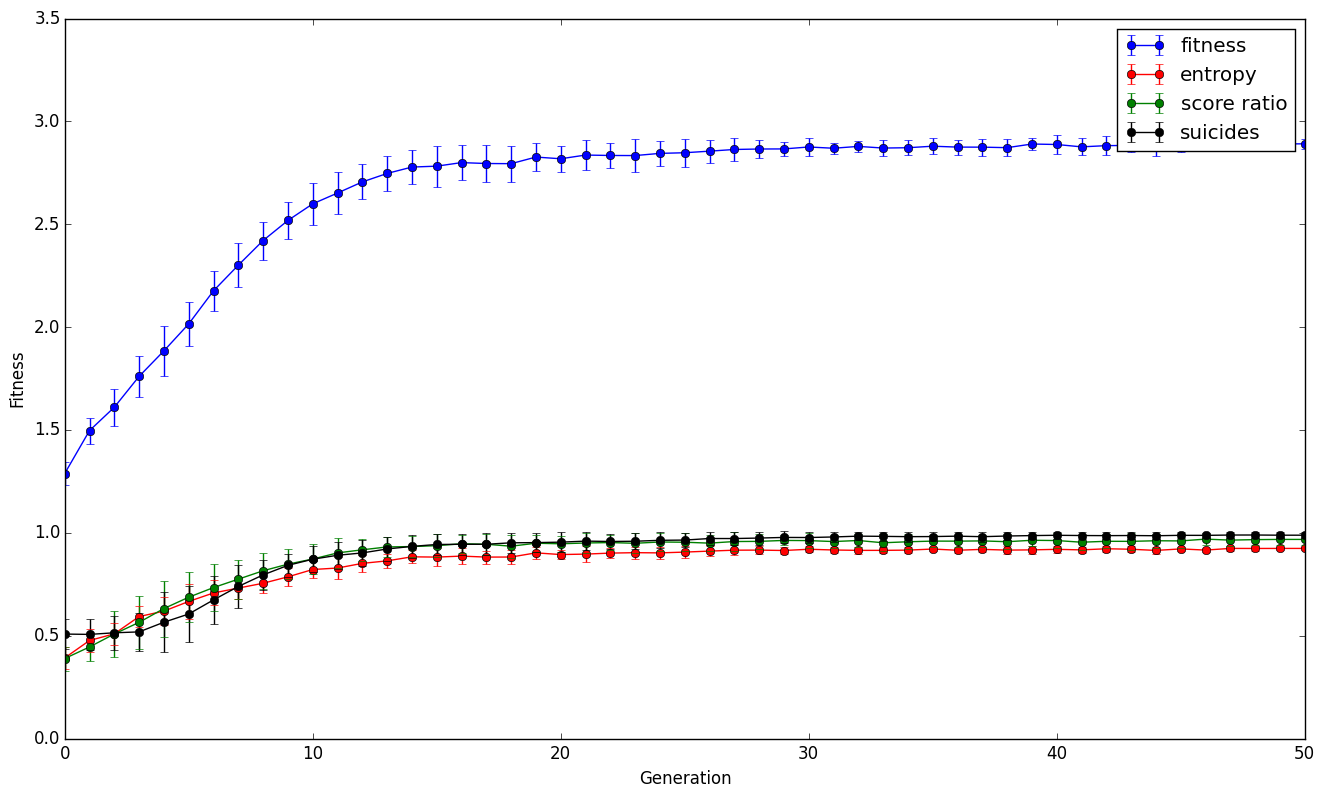
\includegraphics[width=1.0\textwidth]{avg_of_avg}
\caption{Media e deviazione standard delle fitness medie}
\label{fig:avg_of_avg}
\end{figure}

\begin{figure}[tp]
\centering
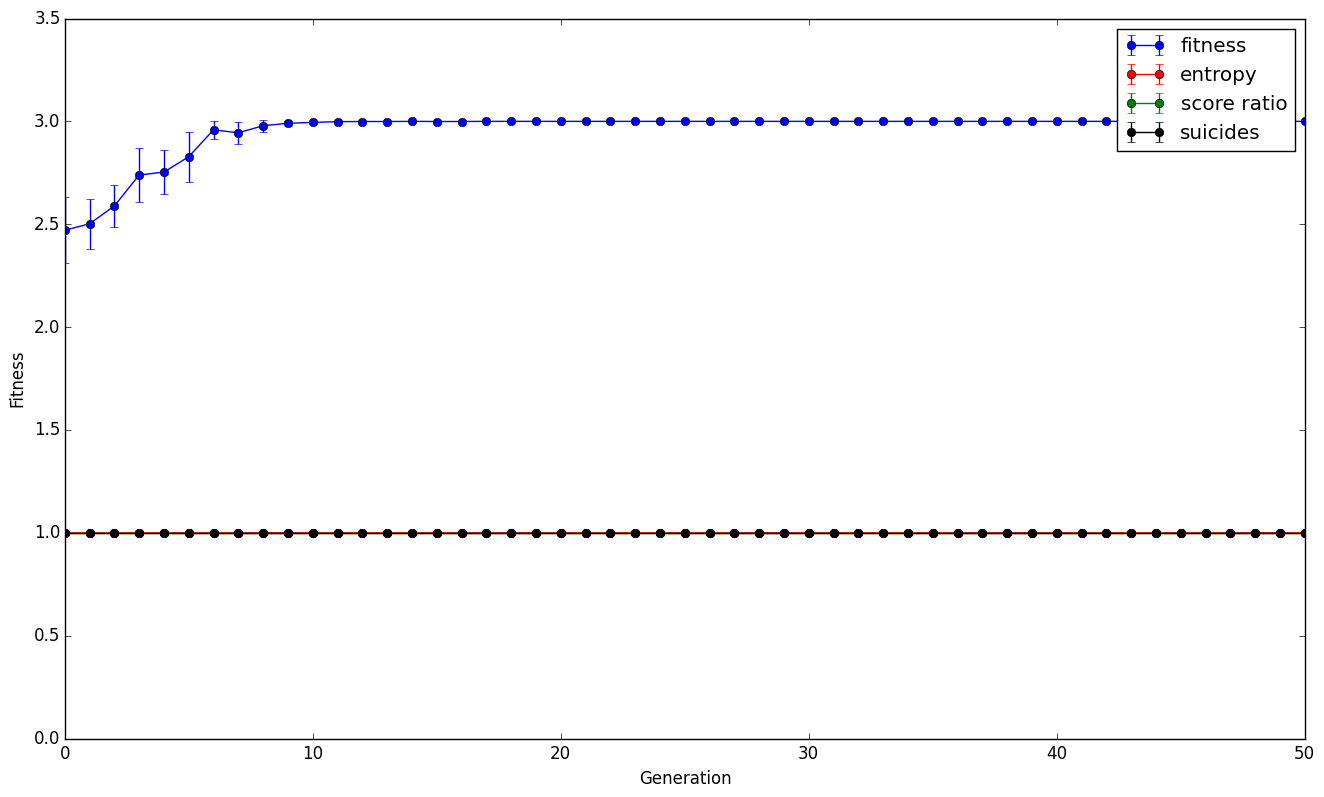
\includegraphics[width=1.0\textwidth]{avg_of_max}
\caption{Media e deviazione standard delle fitness massime}
\label{fig:avg_of_max}
\end{figure}

\subsection{Analisi delle soluzioni}

Nelle 10 prove effettuate dell'esperimento abbiamo ottenuto delle buone prestazioni in media dal punto di vista della fitness, come abbiamo visto nel paragrafo precedente.
Abbiamo quindi deciso di analizzare le caratteristiche principali delle coppie di armi ottenute nelle prove effettuate, in modo tale da valutare quali fossero le caratteristiche che rendono equilibrate queste coppie di armi.
Per visualizzare le caratteristiche emergenti di questi risultati, abbiamo raccolto le popolazioni finali ottenute nelle 10 prove, e le abbiamo sottoposte a un algoritmo di clustering.
Per il clustering abbiamo utilizzato l'algoritmo \emph{DBSCAN} \cite{dbscan:article} con $\epsilon = 0.2$ e $minPts = 5$, attraverso la libreria {P}ython \emph{scikit-learn} \cite{scikit-learn:article}.
Il DBSCAN (\emph{Density-Based Spatial Clustering of Applications with Noise}) è un metodo di clustering basato sulla densità dei punti, che connette regioni dello spazio con una data densità decisa dall'utente.
Il valore della densità dei punti è dettata da due parametri: $\epsilon$ determina la raggiungibilità dei punti all'interno del cluster, mentre \emph{minPts} determina il numero minimo di punti per formare un cluster.
Dopo aver effettuato il clustering abbiamo ottenuto 29 cluster data una popolazione di 1000 individui, cioè la somma dei 100 individui finali ottenuti per ogni prova dell'esperimento effettuata.

Nella figura~\ref{fig:cluster_single_obj_1} mostriamo per ogni singolo parametro come variano le coppie di armi ottenute attraverso il \emph{clustering}. Abbiamo selezionato un campione di 10 cluster, per agevolarne la visualizzazione.
Per ogni parametro delle armi (così come descritti nella nella Sezione~\ref{sec:setting}) andiamo a rappresentare come si comportano le coppie di armi generate; ogni coppia viene indicata con una lettera, e in ciascun coppia le due barre rappresentano rispettivamente la caratteristica in esame della prima e seconda arma della coppia.
Per ogni grafico viene indicato quale caratteristica dell'arma viene rappresentata, e per l'unità di misura di ogni parametro si rimanda alla Sezione~\ref{sec:setting}.
Se prendiamo in considerazione il sotto-grafico rappresentante il \emph{rateo di fuoco} (RoF), è possibile notare che il rateo di fuoco in media è al di sopra dei 2 $proiettili/secondo$: il motivo è la spinta evolutiva data dalla funzione $f_g$ all'interno della funzione di fitness, che premia le armi che riescono a raggiungere il maggior numero di uccisioni nel minor tempo possibile. La soluzione più facile per l'algoritmo è stata quella di aumentare il rateo di fuoco di ciascuna arma.
Nel grafico rappresentante lo \emph{spread} notiamo che le armi mantengono dei valori al di sotto del valore 0.5: le armi minimizzano lo spread con lo scopo di essere più precise, il che aiuta le armi a ottenere il numero di uccisioni prefissato dal \emph{goal score}.
Evidenziamo che i grafici rappresentanti il danno e lo \emph{shotcost} sono spesso complementari: le armi evidentemente cercano di ottimizzare il danno per singolo sparo e di mantenersi equilibrate evitando di massimizzare entrambi le caratteristiche, e quindi per esempio nel caso lo \emph{shotcost} sia al di sotto dei 3 colpi per sparo, il danno viene aumentato fino a 100, come nelle coppie A e I.
Infine nel grafico dedicato al raggio esplosivo dei proiettili (\emph{explosive}) abbiamo in media delle armi che minimizzano questo parametro: la soluzione più facile per minimizzare il numero di suicidi, in modo tale da massimizzare il contributo dato dalla funzione $f_s$, è diminuire il raggio esplosivo, il che comporta una minor probabilità che il bot si suicidi sparando nelle sue vicinanze.
In generale si può apprezzare un'alta varietà di armi generate, il che dimostra una grande potenziale creativo dell'algoritmo.

\begin{figure}[tp]
\centering
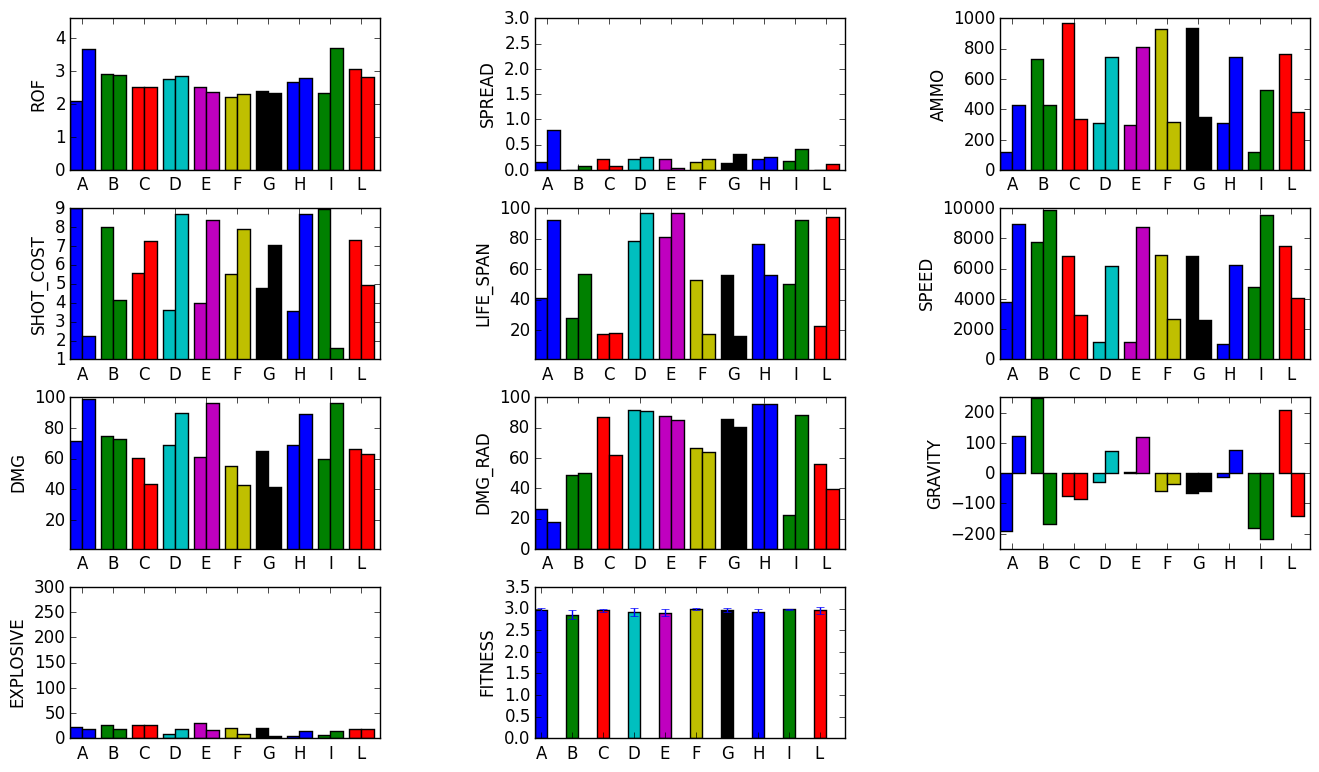
\includegraphics[width=1.2\textwidth, angle=90]{bar_single_obj}
\caption{Grafico a barre delle coppie di armi ottenute con il GA a singolo obiettivo}
\label{fig:cluster_single_obj_1}
\end{figure}

\subsection{Esempi significativi}
\label{sec:esempi_single_obj}

Ora andremo ad analizzare nel dettaglio alcuni esempi di armi generate con l'esperimento descritto in questo capitolo.
Nelle figure~\ref{fig:radar1},~\ref{fig:radar2} mostriamo con dei \emph{radar chart} la media dei parametri delle armi contenute in due cluster scelti tra quelli ottenuti attraverso il clustering descritto nel paragrafo precedente, e un \emph{boxplot} che visualizza come varia l'entropia all'interno del cluster preso in considerazione.
Mentre nelle figure ~\ref{fig:stat_radar_1},~\ref{fig:stat_radar_2} mostriamo tre \emph{boxplot} che vanno ad analizzare il comportamento dei due cluster presi in considerazione rispetto a tre statistiche, calcolate sulla base di 100 simulazioni: la distanza media dei colpi (calcolata in Unreal Unit),  la \emph{Kill Streak}, cioè in media quante uccisioni sono state effettuate di seguito senza mai essere uccisi (calcolata in numero di uccisioni) e precisione media (calcolata come percentuale del rapporto tra numero di colpi che hanno colpito l'avversario e numero di colpi sparati).
Nella figura~\ref{fig:radar1} mostriamo il primo esempio di cluster.
La prima arma ha massimizzato velocità, danno e \emph{lifespan} dei proiettili; inoltre ha uno \emph{shotcost} pari a uno, uno \emph{spread} leggermente più alto della seconda arma e un gravità opposta vicina al massimo negativo. Quest'arma è un'arma di raggio medio-basso, dovuto alla combinazione di gravità e velocità molto alte. La seconda è un'arma a raggio medio-basso, con un'alta concentrazione di proiettili (\emph{shotcost} alto e \emph{spread} quasi nullo) che punta a massimizzare il danno per singolo colpo.
Nella figura \ref{fig:stat_radar_1} possiamo notare una distanza media più alta per la seconda arma, in quanto la prima arma , avendo più \emph{spread} e uno \emph{shotcost} pari a uno, riesce a ottenere degli \emph{hit} solo avvicinandosi all'avversario; per quanto riguarda la precisione, i \emph{boxplot} dimostrano che la seconda arma è più precisa della prima, in quanto la prima, sparando molti proiettili per singolo sparo, ha una maggiore probabilità che alcuni proiettili non colpiscano l'avversario.
Le armi riescono quindi a bilanciarsi in virtù della loro differenza nello \emph{spread} e nello \emph{shotcost}.

\begin{figure}[tp]
\centering
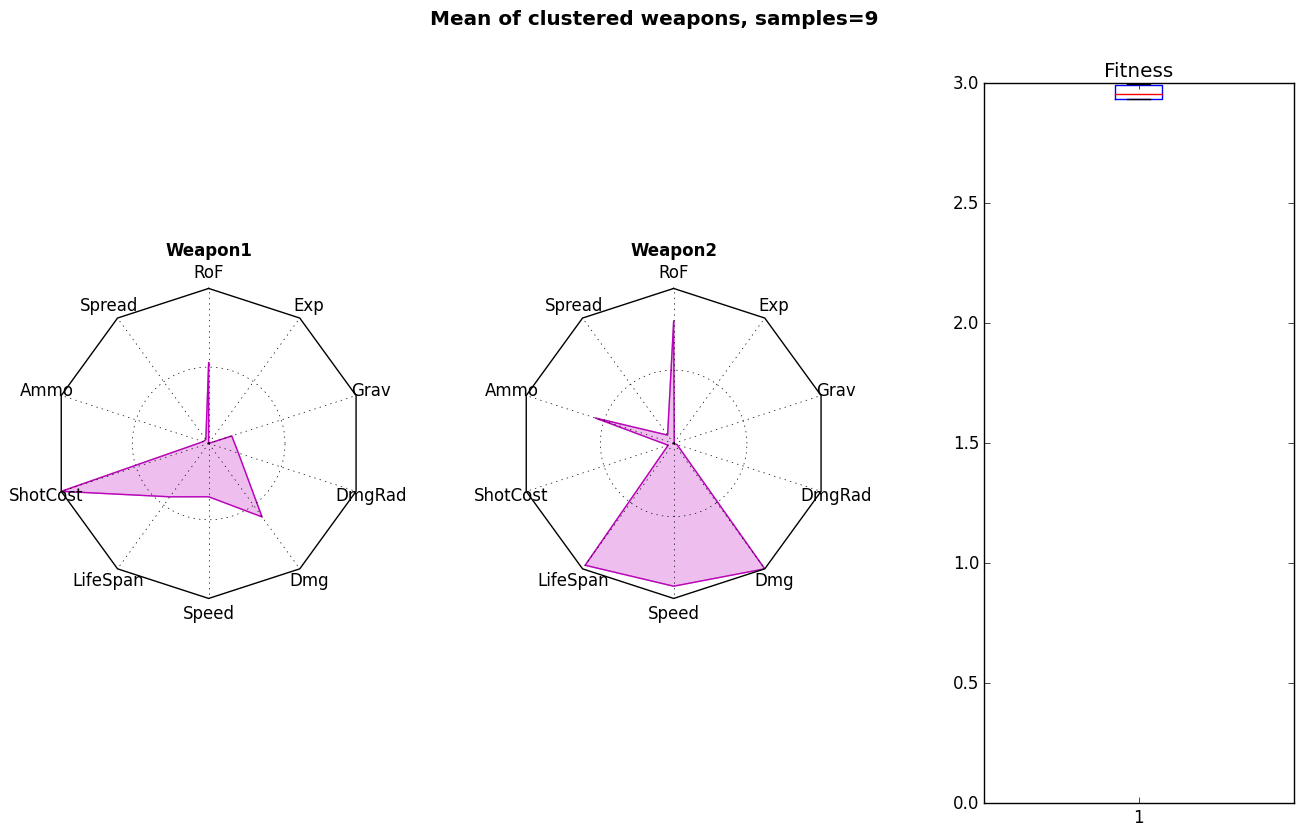
\includegraphics[width=1.0\textwidth]{rad_single_obj_1}
\caption{1° esempio di armi generate con il GA a singolo obiettivo}
\label{fig:radar1}
\end{figure}

\begin{figure}[tp]
\centering
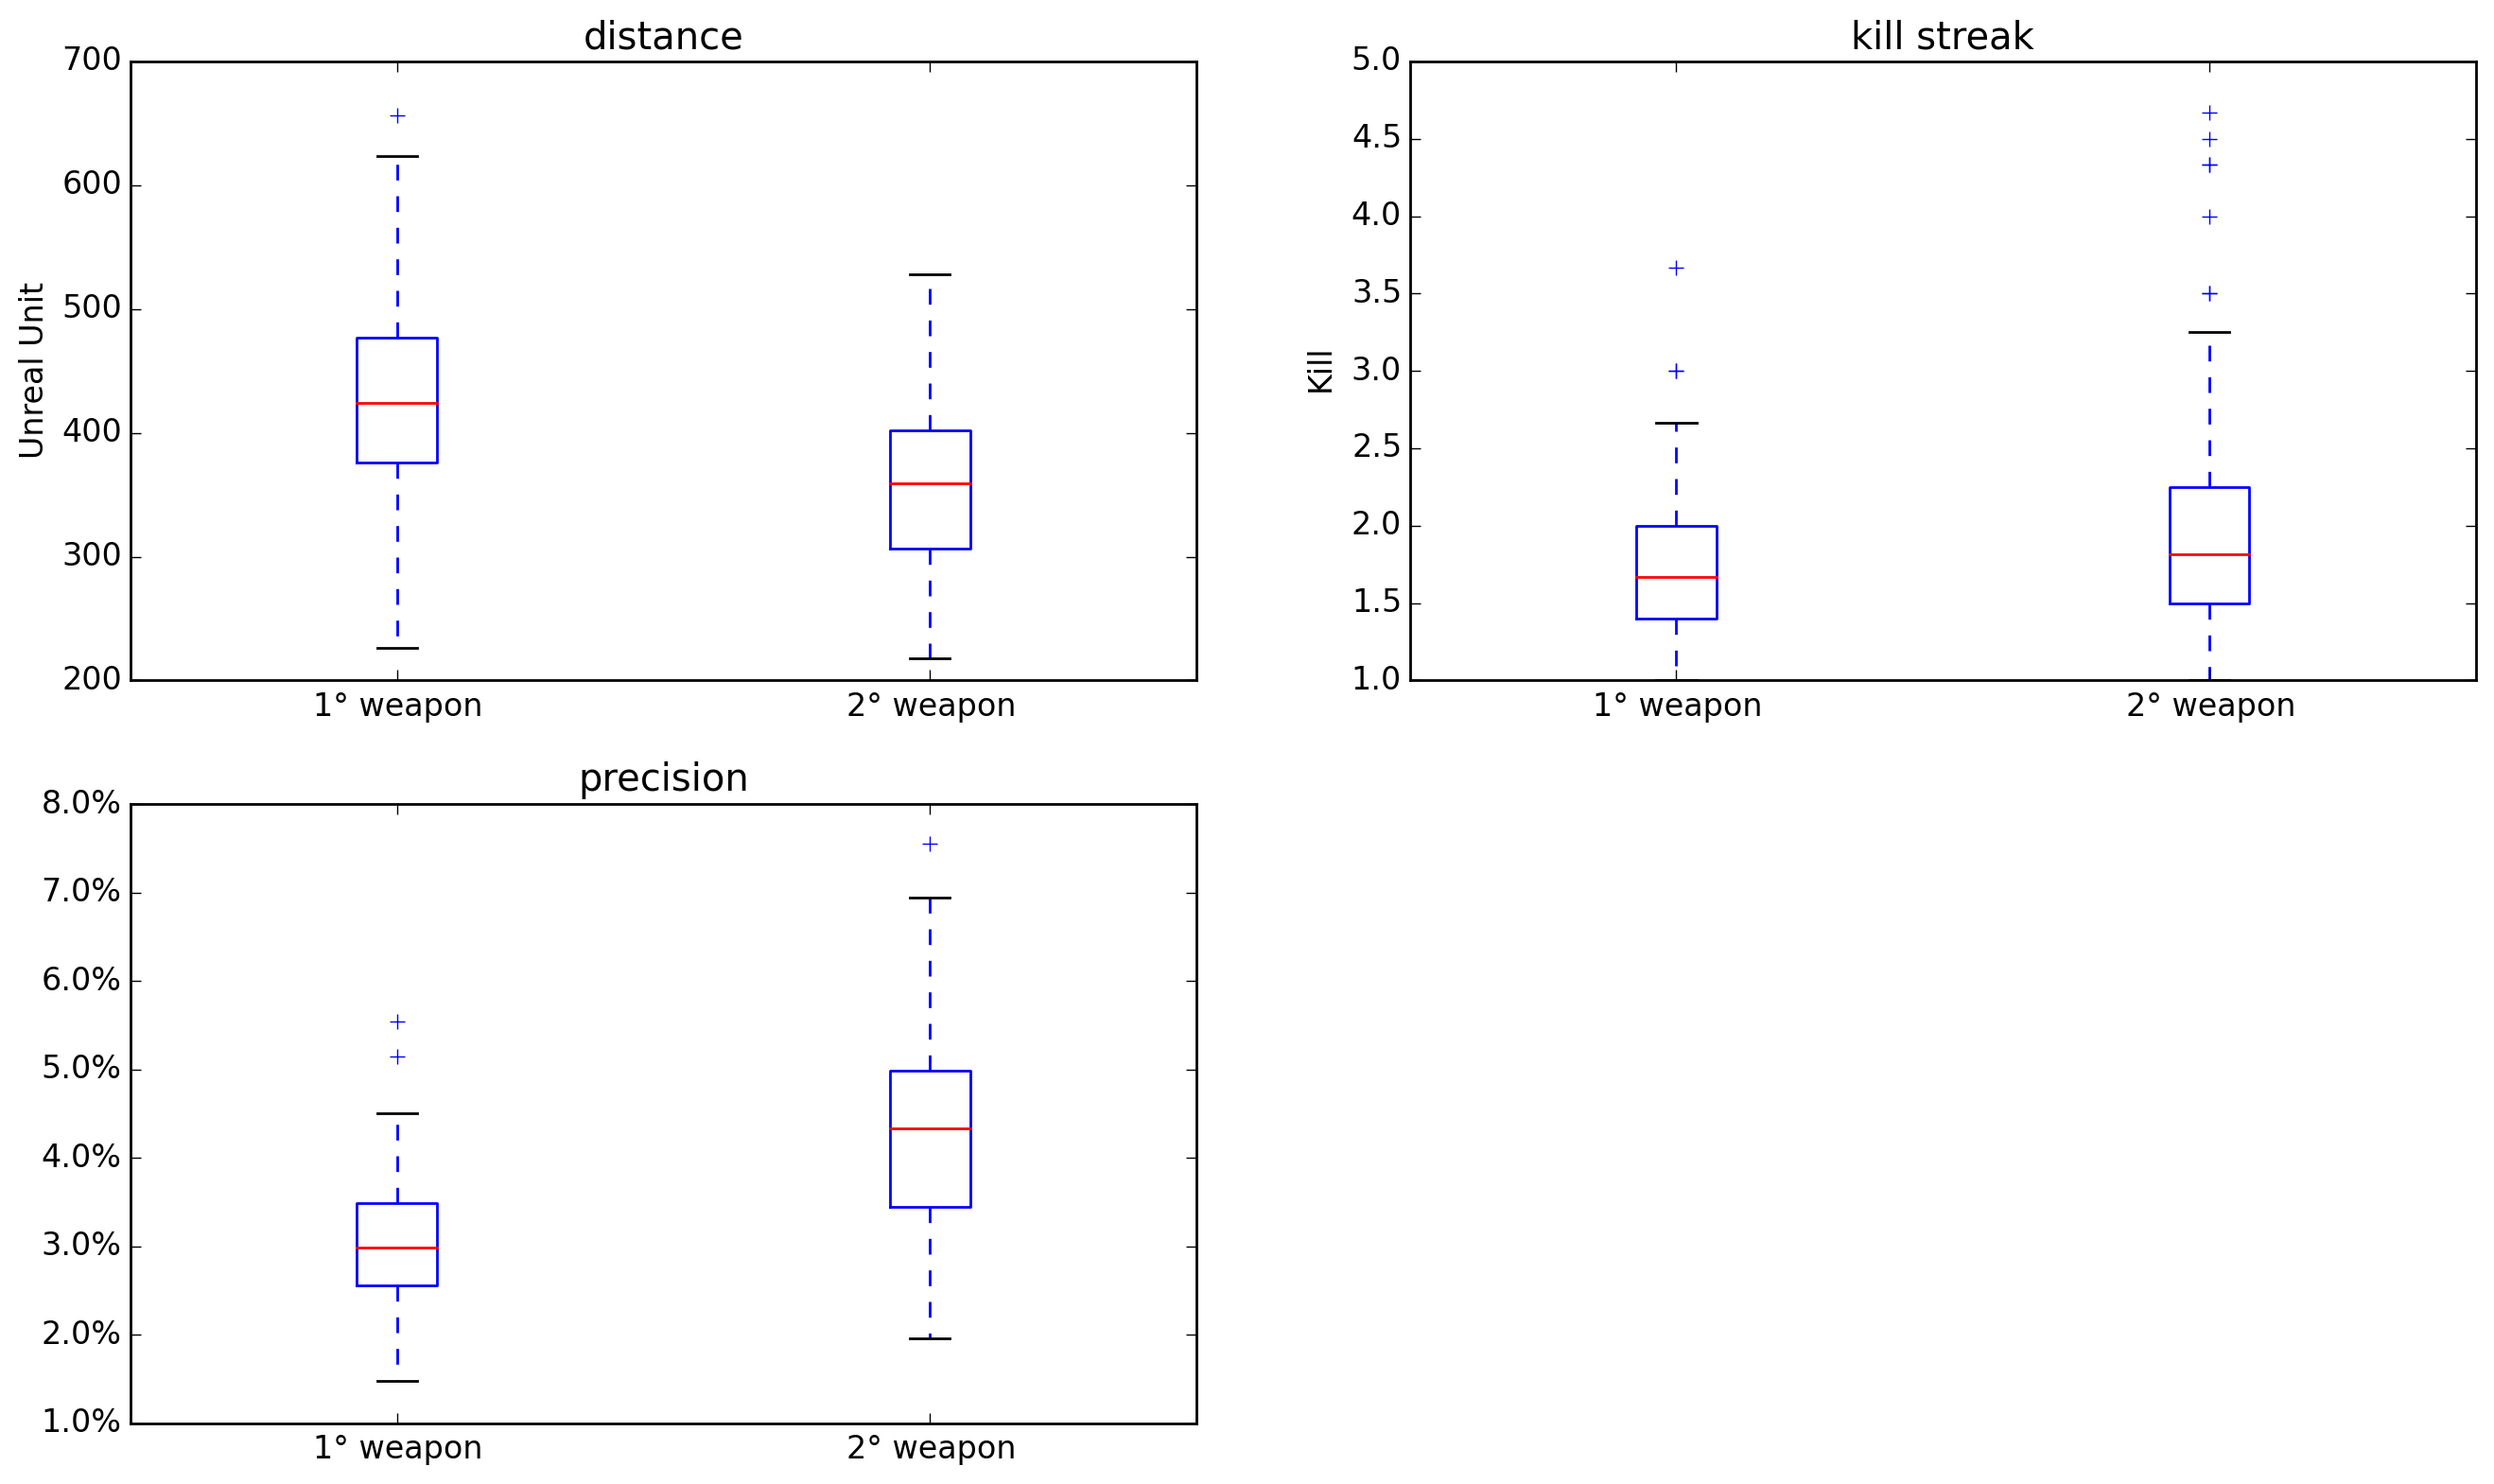
\includegraphics[width=1.0\textwidth]{stat_radar_1}
\caption{statistiche relative al 1° esempio di armi generate}
\label{fig:stat_radar_1}
\end{figure}

Nella figura \ref{fig:radar2} prendiamo in considerazione una seconda coppia di armi. In questo caso la prima arma ha un rateo di fuoco medio, pochissimo \emph{spread}, uno \emph{shotcost} molto alto e un gravità elevata. Ma la seconda arma è molto più interessante: un rateo di fuoco medio, uno \emph{spread} minimo, uno \emph{shotcost} pari a 5 e una combinazione di \emph{speed} e \emph{life span} molto elevati. Questa è un'arma a lungo raggio, molto simile a un fucile da cecchino. Queste armi riescono a bilanciarsi in virtù della loro diverso range di fuoco: la prima è appunto un'arma molto potente sulle corte distanze, mentre la seconda è più adatta alle lunghe distanze. 
Come possiamo vedere dalla figura \ref{fig:stat_radar_2} le distanze coperte dalla seconda arma sono molto più alte, dove abbiamo un massimo a 1200 UU. Anche la precisione della seconda arma è più alta, nonostante lo \emph{spread} quasi identico delle due armi: questo è giustificato dal fatto che il bot potendo sparare da distanze più grandi ha un tempo maggiore per prendere la mira. Infine è possibile vedere che la \emph{kill streak} della seconda arma è leggermente maggiore: questo è sempre dovuto al range più elevato di quest'ultima, che permette di concatenare più uccisioni senza essere colpito dall'avversario.

I due esempi analizzati dimostrano la creatività dell'algoritmo che è riuscito a generare armi molto diverse e interessanti.

\begin{figure}[tp]
\centering
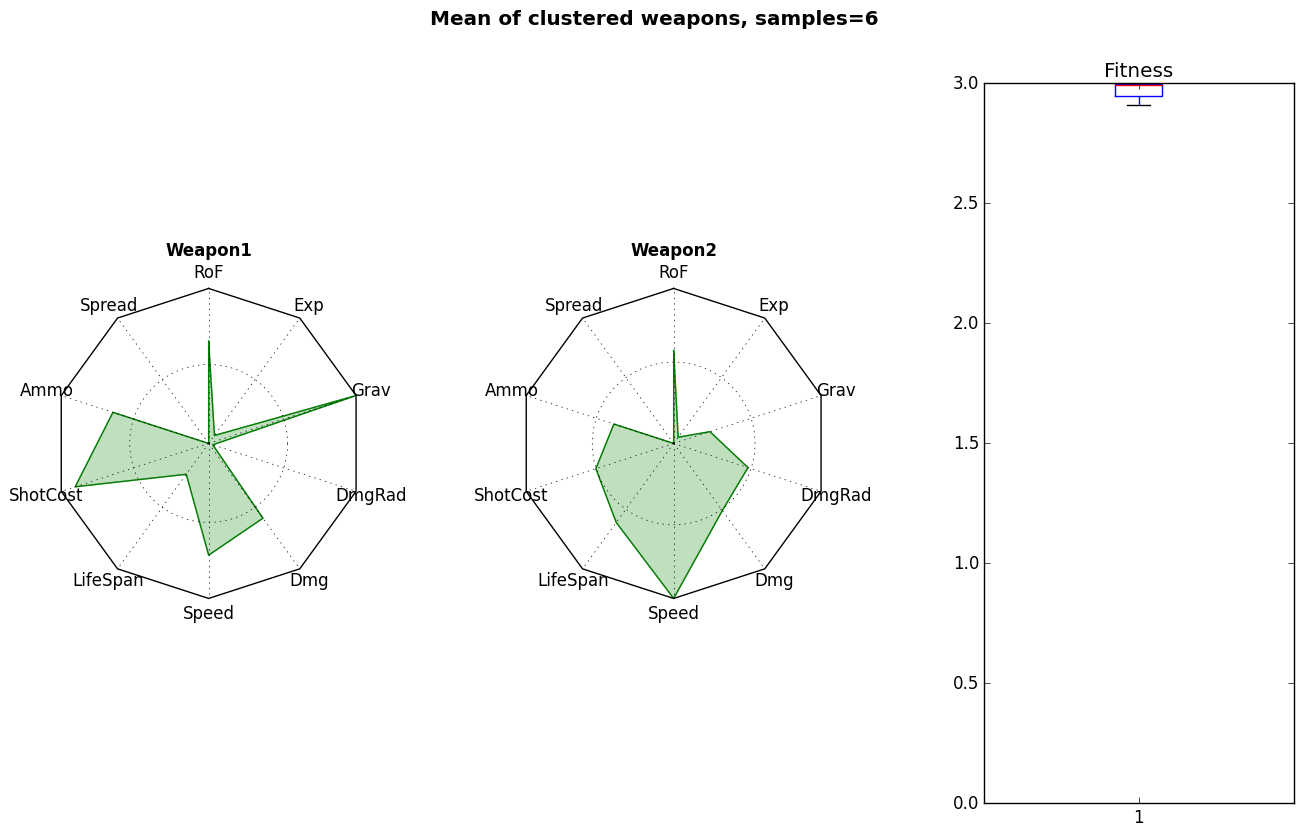
\includegraphics[width=1.0\textwidth]{rad_single_obj_2}
\caption{2° esempio di armi generate con il GA a singolo obiettivo}
\label{fig:radar2}
\end{figure}

\begin{figure}[tp]
\centering
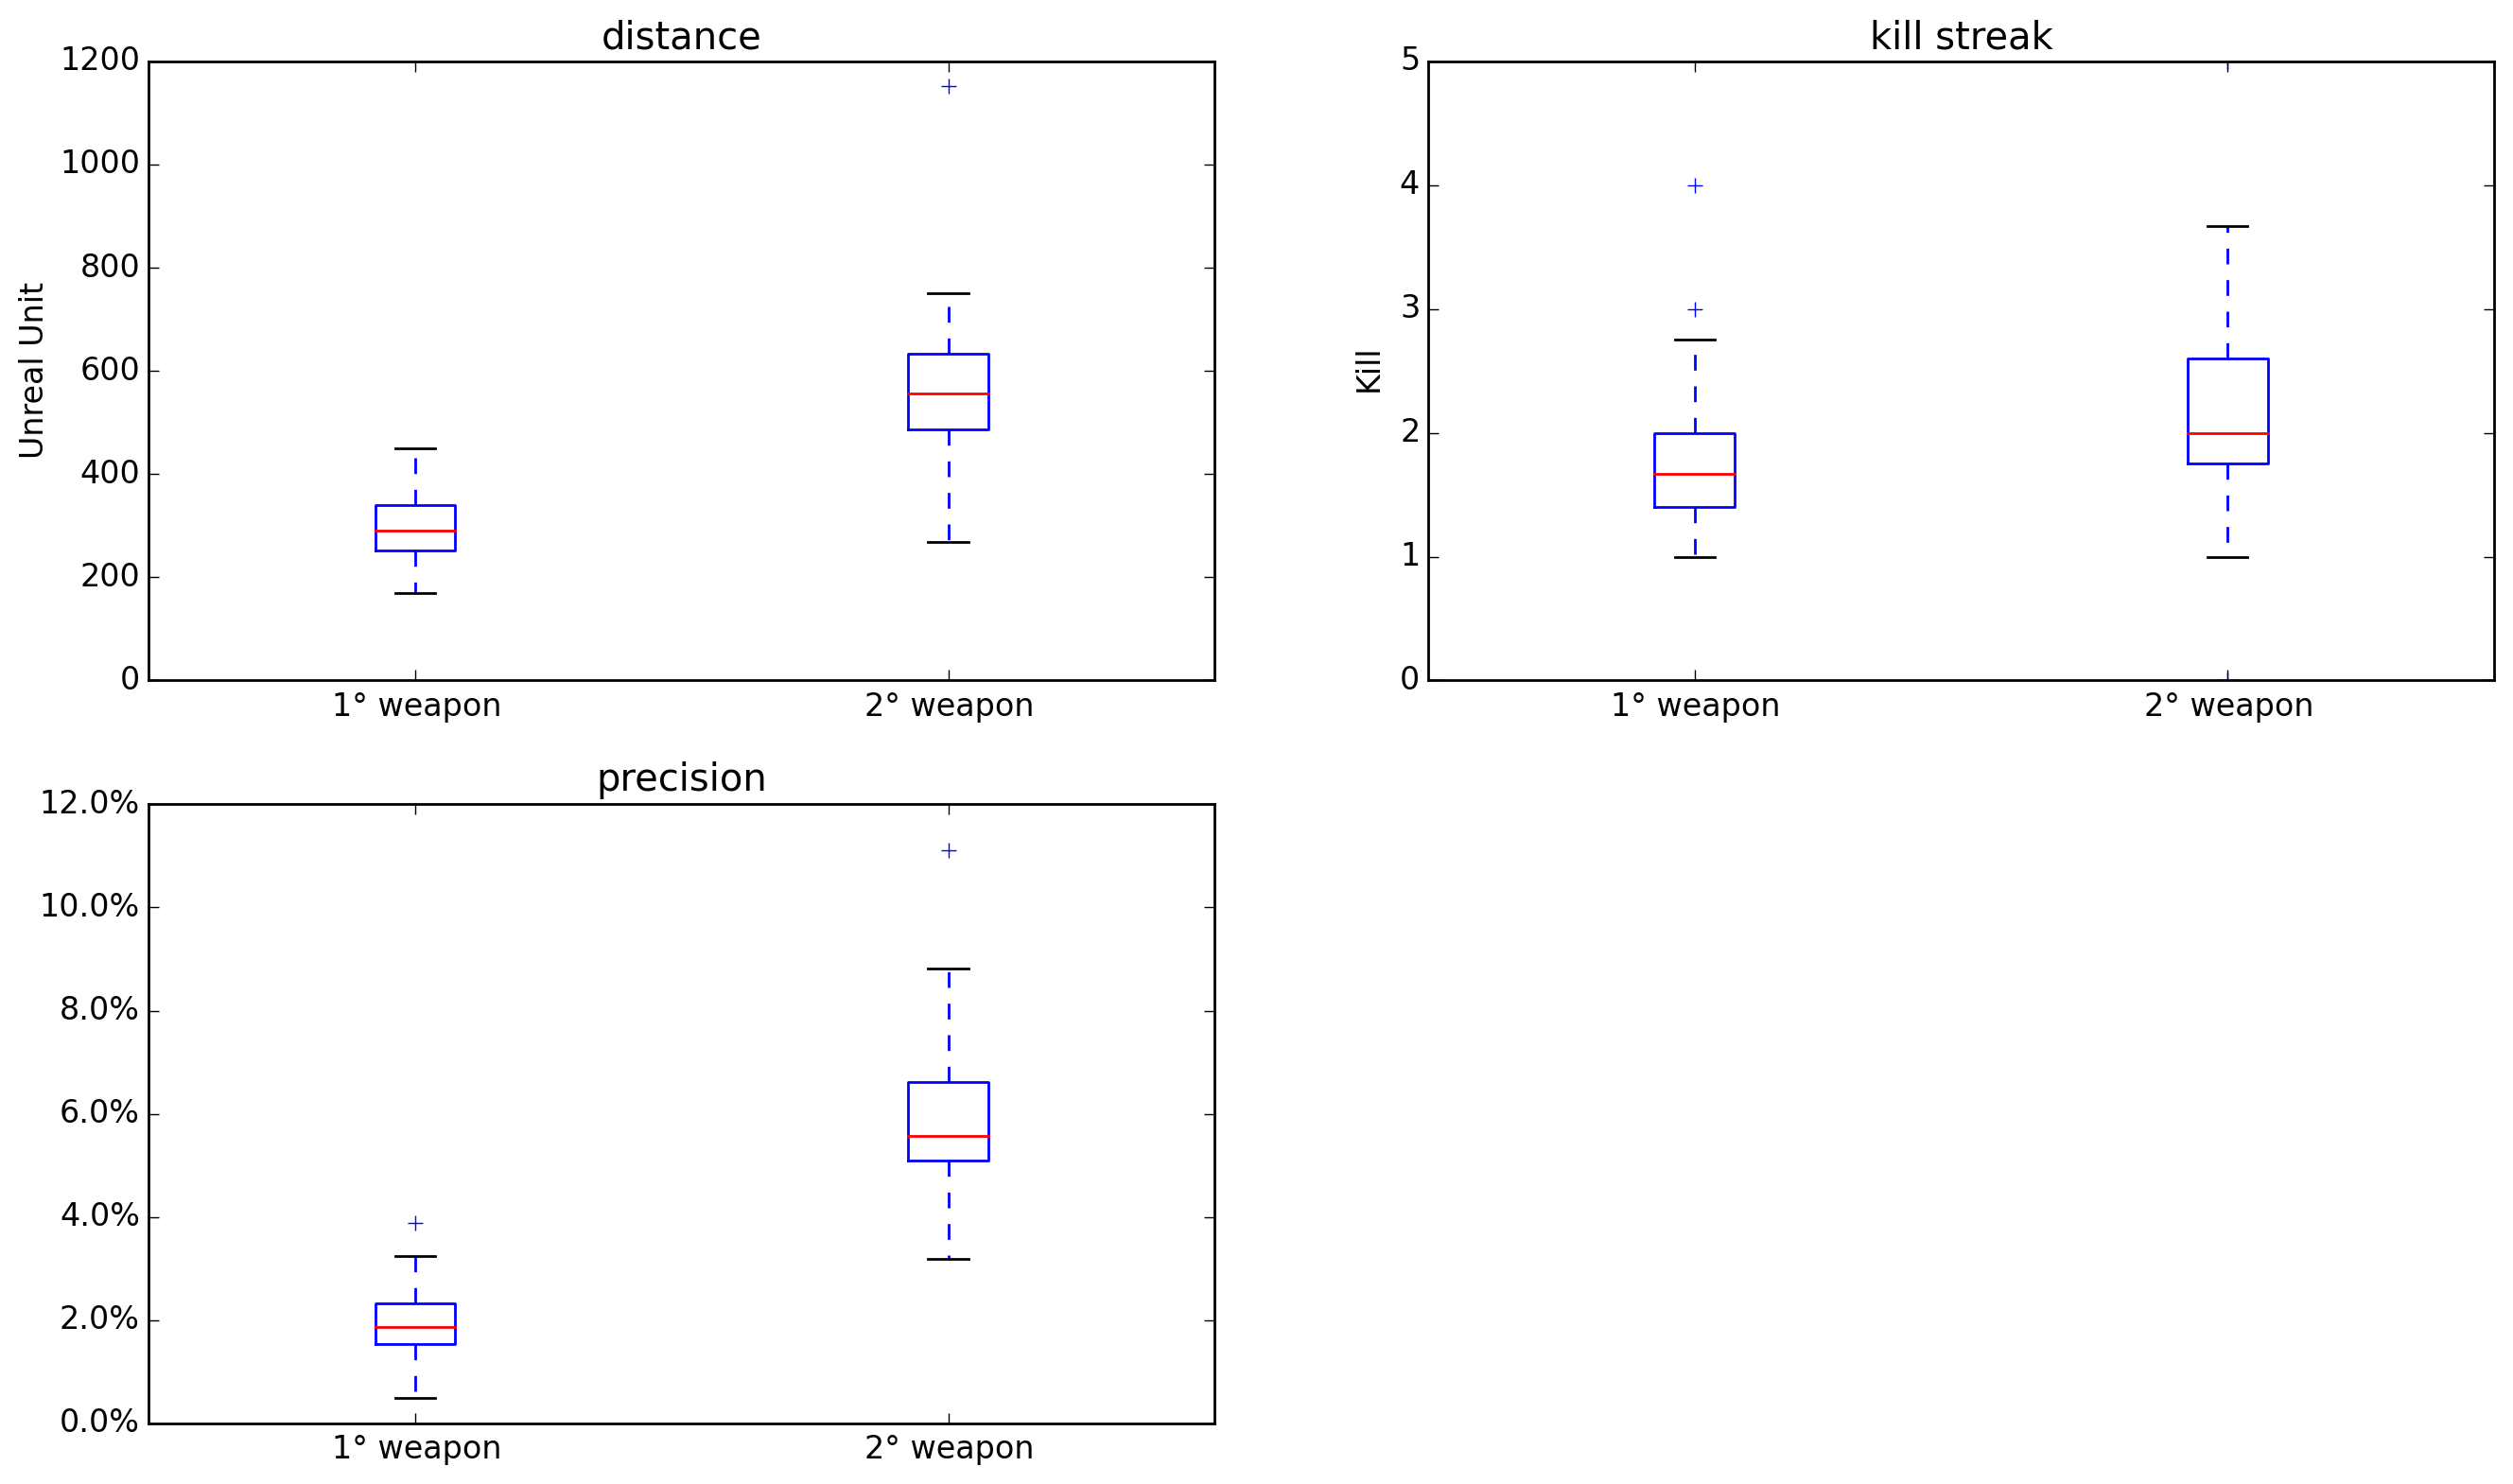
\includegraphics[width=1.0\textwidth]{stat_radar_2}
\caption{statistiche relative al 2° esempio di armi generate}
\label{fig:stat_radar_2}
\end{figure}


\section{Validazione}
\label{sec:error_single_obj}
Nella Sezione \ref{sec:goal_score} abbiamo evidenziato come le simulazioni effettuate in UT3 abbiano un errore di valutazione nel caso che il \emph{goal score} sia 20.
Per validare i risultati ottenuti dalle 10 prove effettuate in questo esperimento, abbiamo rivalutato la fitness delle 10 popolazioni finali con un \emph{goal score} più ampio, pari a 40, il che da una stima più precisa del vero valore di fitness delle coppie di armi e ci permette di valutare se le coppie di armi che abbiamo generato sono effettivamente bilanciate.
Quindi abbiamo cambiato la configurazione delle simulazioni: il limite delle uccisioni totali per partita è stato cambiato con 40, e il tempo limite delle partite è stato impostato a 2400 secondi.

I risultati mostrano un errore medio, calcolato come differenza tra valutazione della fitness con \emph{goal score} pari 40 e \emph{goal score} pari a 20, di $-0.035$ e una deviazione standard di $0.27$.
L'errore medio è relativamente piccolo e negativo, dovuto principalmente a delle valutazione pessimistiche dell'entropia delle coppie di armi con \emph{goal score} pari a 20, mentre i contributi dati dalle due funzioni secondarie, $f_t$ e $f_s$ hanno un errore nullo rispetto alla valutazione con \emph{goal score} pari a 20.
Solo per alcuni individui però abbiamo una differenza pari a -2, il che giustifica il valore della deviazione standard: questo è dovuto a delle simulazioni in cui i bot non sono riusciti a raggiungere un numero sufficiente di uccisioni, il che ha portato a una valutazione completamente errata. Infatti può capitare che alcuni rari casi le simulazioni siano \emph{difettose} per la velocità maggiorata a cui sono eseguite, come abbiamo descritto nella Sezione 3.3.1, e questo comporta un numero di uccisioni minore rispetto a una simulazione corretta. In questi casi la rivalutazione non è affidabile, in quanto sia il valore dell'entropia sia quello d $f_t$ saranno molto diversi da una simulazione senza errori.

Nella figura~\ref{fig:single_obj_err} visualizziamo nel dettaglio la media e la deviazione standard dell'errore (calcolato come differenza tra la valutazione con \emph{goal score} pari a 40 e la valutazione con \emph{goal score} pari a 20) per ogni popolazione finale ottenuta nei 10 esperimenti, e come si può vedere le considerazioni fatte precedentemente valgono anche per le singole popolazioni: qualitativamente possiamo notare un errore medio in generale molto piccolo e una deviazione standard sempre molto elevata rispetto all'errore medio, dovuto ai casi di simulazione errata.

\begin{figure}[tp]
\centering
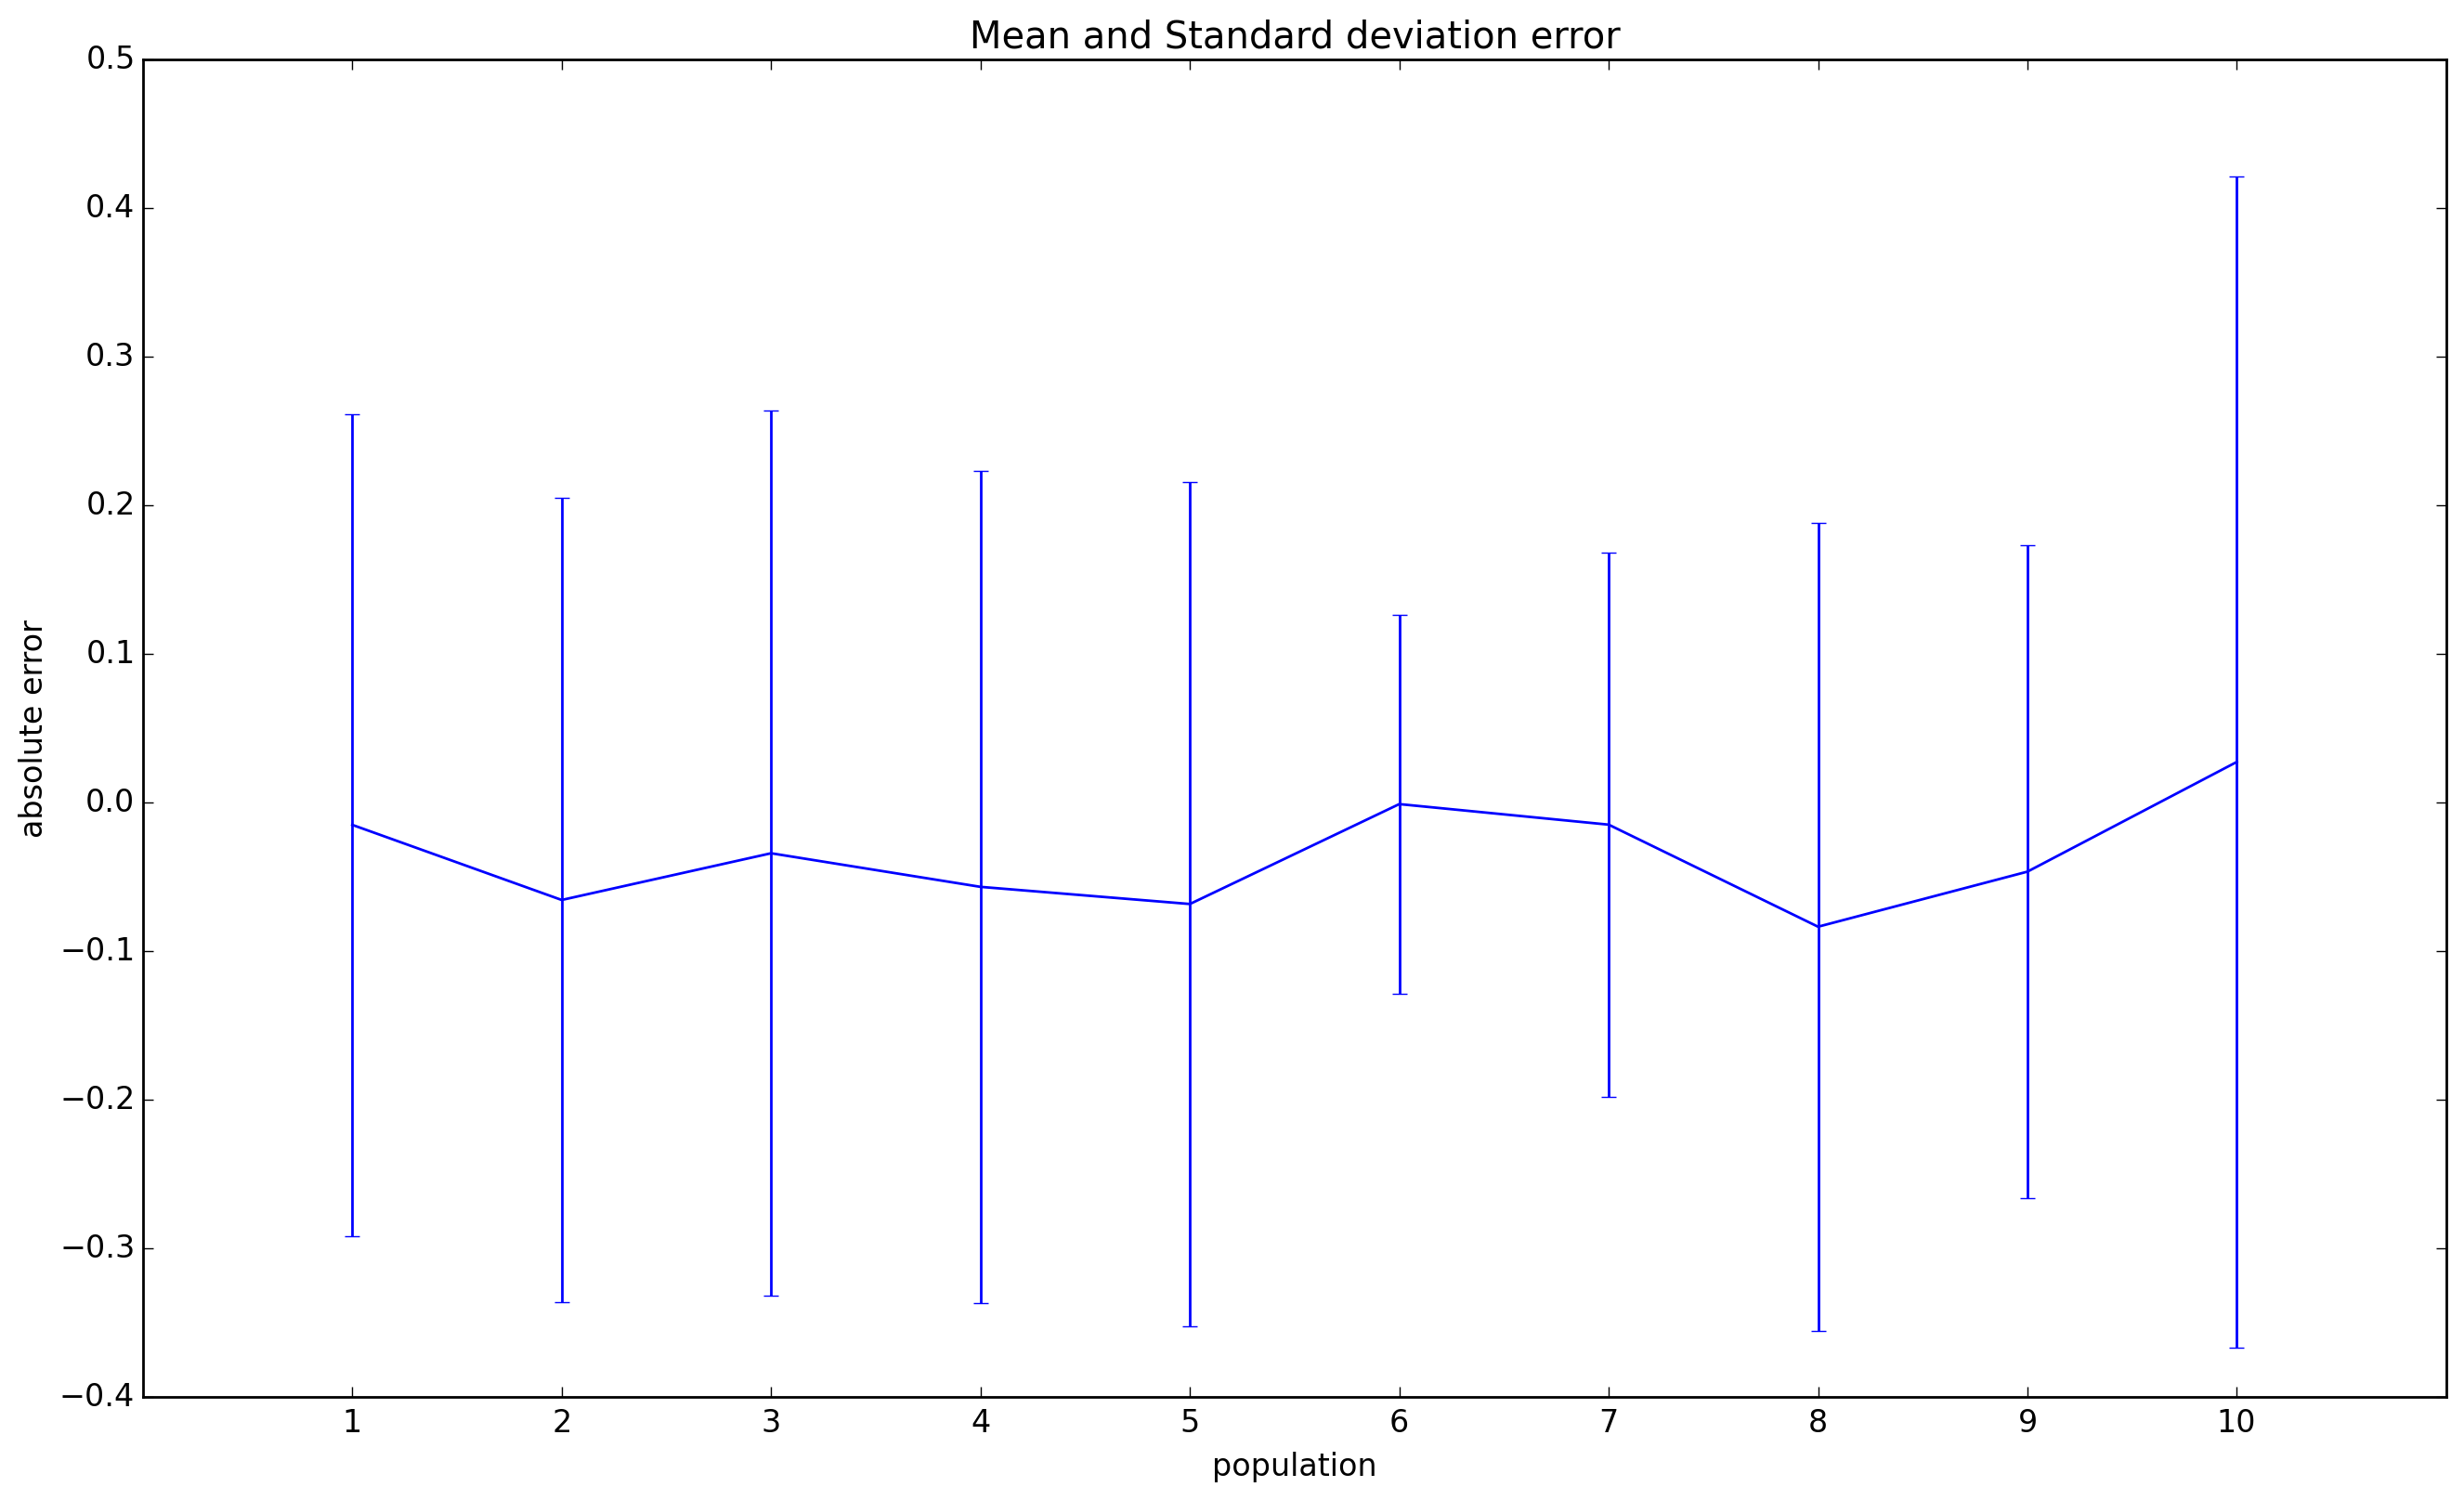
\includegraphics[width=1.0\textwidth]{single_obj_error}
\caption{media e deviazione standard dell'errore ottenuto con GA a singolo obiettivo}
\label{fig:single_obj_err}
\end{figure}

\section{Sommario}
In questo capitolo abbiamo condotto degli esperimenti sulla generazione di armi bilanciate senza vincoli aggiuntivi.
Nella Sezione 4.1 introduciamo gli obiettivi di questi esperimenti e la descrizione della funzione di fitness.
Nella Sezione 4.2 descriviamo i risultati ottenuti ed analizziamo alcuni esempi di armi generate.
Nella Sezione 4.3 infine andiamo a mostrare l'errore ottenuto rivalutando i risultati ottenuti con un \emph{goal score} pari a 40.

\chapter{Bilanciamento automatico di un'arma obiettivo}
In questo capitolo andremo a descrivere uno strumento che possa bilanciare automaticamente un'arma obiettivo data un'arma fissa.
Questo può permettere ai game designer di costruire delle armi \emph{ad hoc} e poi utilizzare questo strumento per bilanciare le armi automaticamente.
Per esempio il game designer potrebbe progettare un'arma con alcune caratteristiche volute, e poi lasciare all'algoritmo genetico il compito di mettere a punto i parametri in modo tale che sia un'arma equilibrata.
Quindi per valutare come si comporta in questo scenario applicativo l'algoritmo genetico, abbiamo scelto due armi presenti nel gioco \emph{Unreal Tournament III}, e dopo aver selezionato l'arma che risultava aver uno svantaggio in termini di uccisioni ottenute nelle simulazioni, abbiamo provato a bilanciarla contro quella più forte.
Inizialmente andremo a descrivere il design sperimentale scelto per questo tipo di esperimento.
Successivamente andremo ad analizzare i risultati ottenuti nelle prove dell'esperimento effettuate e infine andremo a validare i risultati con una valutazione più precisa del bilanciamento.

\section{Design Sperimentale}
Per poter valutare come l'algoritmo genetico si comporta nel bilanciare un'arma obiettivo contro un'arma fissa, abbiamo scelto due armi presenti in \emph{Unreal Tournament III}: il \emph{Flak} e il \emph{Rocket Launcher}.
Queste due armi sono implementate nella logica di gioco scritta con \emph{UnrealScript}: abbiamo quindi estratto i parametri principali delle due armi e le abbiamo rappresentate secondo la rappresentazione descritta nella Sezione \ref{sec:setting}.
Questo \emph{rappresentazione} delle due armi comporta alcune semplificazioni: le armi presenti in UT3 hanno alcune funzioni e tipo di modalità di fuoco particolari per ogni arma,  per esempio ogni arma ha due modalità di fuoco, alcune armi hanno il \emph{lock-on} automatico, ecc.; queste caratteristiche specifiche di alcune armi potrebbero comportare delle leggere differenze rispetto alla nostra implementazione, ma per rendere più generale possibile la rappresentazione delle armi abbiamo dovuto semplificare alcune funzionalità.
Ora andremo a descrivere l'algoritmo implementato per questo esperimento, i parametri scelti per la simulazione, la rappresentazione e la funzione di fitness.

\subsection{Algoritmo e Parametri Sperimentali}
\label{sec:nsga2}
In questo esperimento vogliamo bilanciare un'arma obiettivo: quindi abbiamo formalizzato la risoluzione di questo problema con un algoritmo multiobiettivo, dove il primo obiettivo è il bilanciamento dell'arma rispetto all'arma fissa data, e il secondo obiettivo è la minimizzazione della distanza euclidea dei parametri dell'arma generata e i parametri dell'arma obiettivo.
In questo modo indichiamo all'algoritmo genetico che deve esplorare lo spazio delle armi nelle immediate vicinanze dell'arma obiettivo, e che deve trovare quali sono i parametri da modificare per rendere quest'arma equilibrata rispetto all'arma fissa.
Abbiamo quindi dovuto scegliere un'implementazione di algoritmo genetico \emph{multiobiettivo}: la nostra scelta è ricaduta sull'implementazione \emph{NSGA-II} \cite{nsga2:article}, attraverso la libreria {P}ython  DEAP\cite{deap:article}.
Gli operatori genetici scelti per questo esperimento sono i seguenti:  per il crossover abbiamo scelto il \emph{simulated binary crossover} con probabilità 0.9; per la mutazione abbiamo scelto la \emph{simulated binary mutation} con probabilità 0.1; e infine come selezione abbiamo scelto la \emph{tournament selection} a due individui.
La probabilità di \emph{crossover} è più alta della probabilità usata per l'esperimento con GA a singolo obiettivo (capitolo 3) perché con l'\emph{NSGA-II} abbiamo un forte \emph{elitismo}, cioè all'interno del processo di selezione degli individui per formare una nuova popolazione, un certo di numero individui che hanno ottenuto delle fitness molto performanti nella generazione precedente, vengono direttamente inseriti nella popolazione successiva. Infatti, in ogni generazione dell'algoritmo, vengono mantenute due diverse popolazioni, una costituita dagli individui della popolazione precedente, e un'altra, chiamata \emph{offspring}, creata mediante la selezione e gli operatori genetici come nell'implementazione che abbiamo descritto nella Sezione \ref{sec:SBPCG}. Quindi l'algoritmo, dopo aver calcolato la fitness della popolazione \emph{offspring}, applica un \emph{fast non-dominated sorting}\cite{nsga2:article} all'unione delle due popolazioni, da cui vengono selezionati un numero di individui pari alla quantità di elementi nella popolazione iniziale in base al loro ordine ottenuto con il \emph{fast non-dominated sorting}.

La rappresentazione consiste in un vettore di 10 parametri, che rappresenta l'arma da bilanciare. Ogni volta che client vuole testare l'arma generata, i parametri di quest'ultima vengono inviati al server assieme ai parametri dell'arma fissa contro la quale vogliamo testare il bilanciamento.

La simulazione avviene in una mappa di piccole dimensioni, \emph{DM-Biohazard} e nella modalità \emph{Deathmatch}. La configurazione della partita è la seguente: ai bot viene assegnata una skill pari a 7 (cioè il massimo), un limite di uccisioni totali (\emph{goal score}) pari a 20 e un tempo limite di 1200 secondi.
Dopo aver fatto alcuni test abbiamo considerato ottimali un numero di generazioni pari a 50 e una popolazione composta da 50 individui, in quanto in questo caso il numero di parametri è 10, quindi metà rispetto alla rappresentazione usata nel Capitolo 4.
La durata media per singola prova dell'esperimento si è attestata sulle 8 ore.

\subsection{Funzione di Fitness}

Avendo scelto un algoritmo multiobiettivo abbiamo progettato due diverse funzioni di fitness, che formalizzano i due obiettivi di questo esperimento.
Il primo obiettivo è la massimizzazione del bilanciamento: questa funzione è la medesima descritta nella Sezione \ref{subsec:fitness}.
Il secondo obiettivo invece è la minimizzazione della distanza euclidea dall'arma obiettivo: 
\begin{equation}
f_d = \sqrt{ \sum_{i=1}^{10} (p_i - o_i)^2}
\end{equation}
dove $p_i$ sono i parametri dell'arma generata e $o_i$ sono i parametri dell'arma obiettivo. 
In questo modo indichiamo all'algoritmo che deve ricercare lo spazio di armi nelle immediate vicinanze dell'arma obiettivo, con lo scopo finale di trovare l'arma con il miglior \emph{trade-off} tra bilanciamento e distanza dall'arma obiettivo.
Quindi gli obiettivi sono i seguenti:
\begin{enumerate}
\item Bilanciamento -- $f_e + f_g + f_s$
\item Distanza euclidea dall'arma obiettivo -- $f_d$
\end{enumerate}

\subsection{Armi scelte per l'esperimento}
Come abbiamo detto precedentemente, abbiamo deciso di selezionare due armi di UT3: il \emph{Flak} e il \emph{Rocket Launcher}.
Per valutare quale delle due armi dovessimo usare come arma obiettivo da bilanciare e quale come arma fissa, abbiamo deciso di simulare 10 partite per vedere quali delle due fosse svantaggiata rispetto all'altra.
Nella figura \ref{fig:flak_vs_rocket} mostriamo attraverso dei \emph{radar chart} come abbiamo deciso di rappresentare le caratteristiche delle due armi con la nostra rappresentazione, in particolare a sinistra mostriamo i parametri scelti per l'arma \emph{Rocket Launcher} e a destra i parametri per l'arma \emph{Flak}.
Nella figura \ref{fig:kill_rocket_vs_flak} mostriamo a sinistra il \emph{boxplot} delle uccisioni ottenute dal \emph{Rocket Launcher} e a destra il \emph{boxplot} delle uccisioni ottenute dal \emph{Flak}, dati raccolti dalle 10 simulazioni effettuate assegnando al primo bot il \emph{Rocket Launcher} e a l secondo bot il \emph{Flak}. Come si nota, il \emph{Flak} è svantaggiato rispetto al \emph{Rocket Launcher}, e quindi abbiamo deciso di selezionare come arma da bilanciare il \emph{Flak} e come arma fissa il \emph{Rocket Launcher}.

\begin{figure}[htp]
\centering
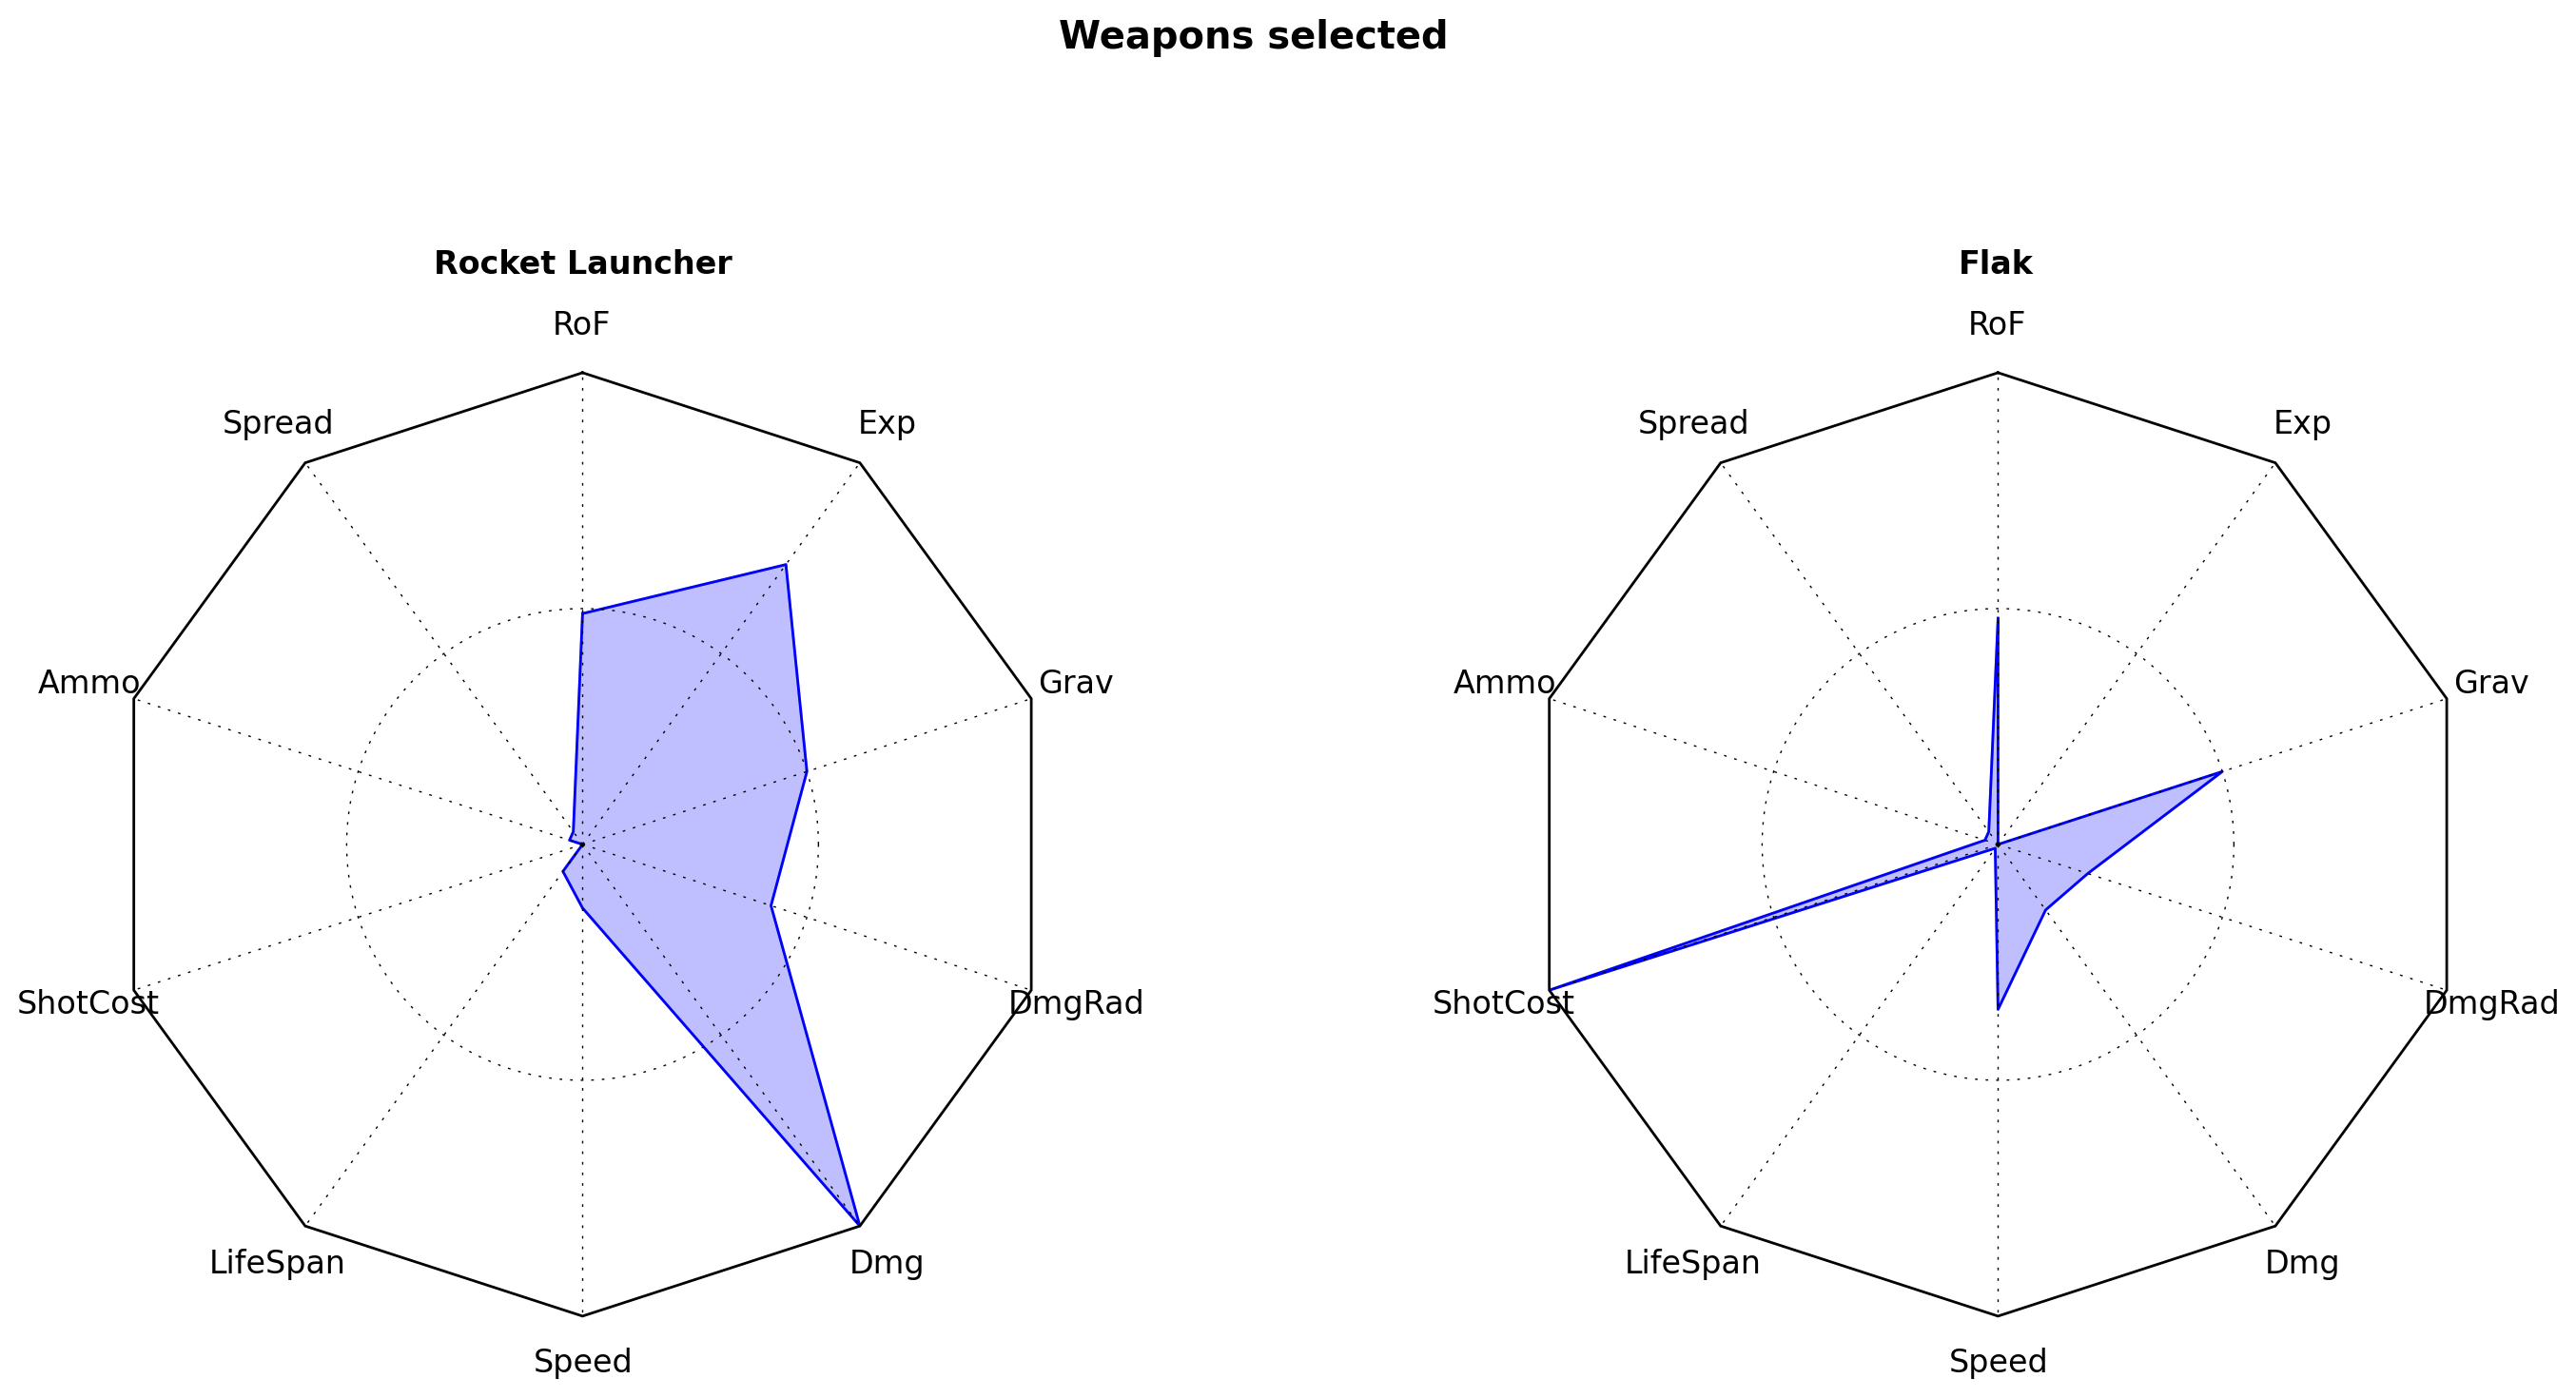
\includegraphics[width=1.0\textwidth]{flak_vs_rocket}
\caption{\emph{radar chart} dell'arma \emph{Rocket Launcher} e dell'arma \emph{Flak}}
\label{fig:flak_vs_rocket}
\end{figure}

\begin{figure}[htp]
\centering
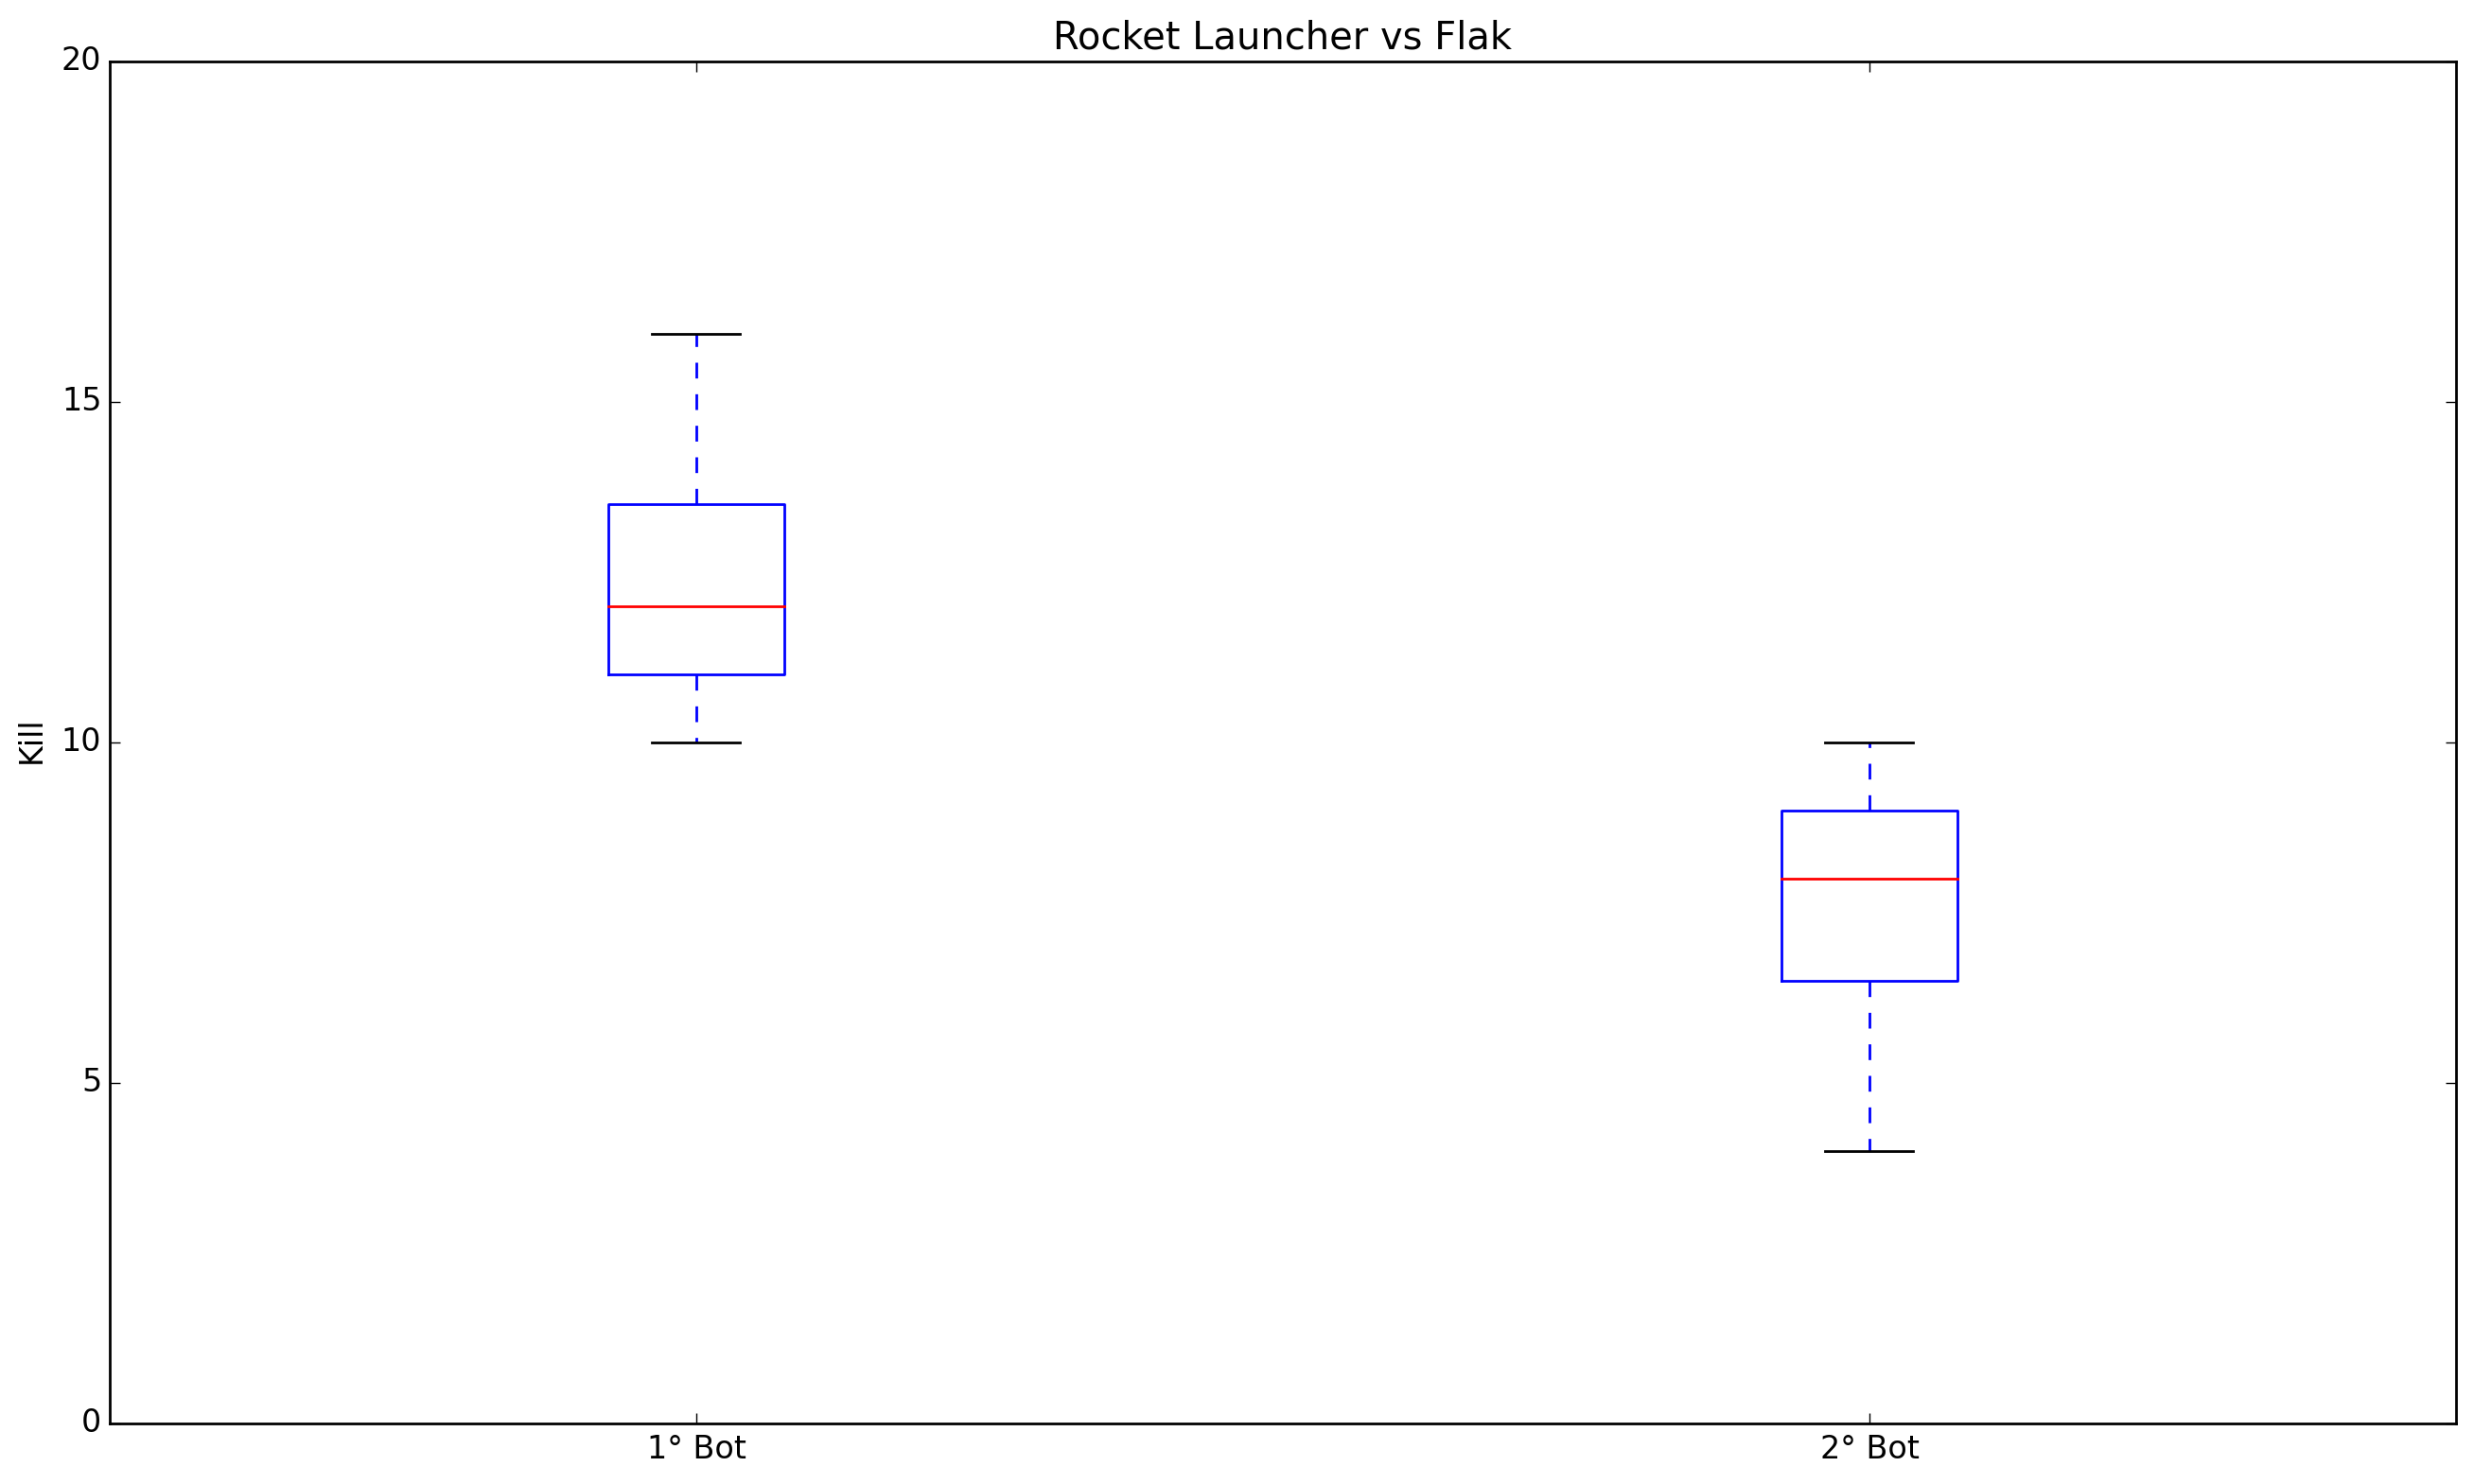
\includegraphics[width=1.0\textwidth]{kill_rocket_vs_flak}
\caption{\emph{boxplot} delle uccisioni ottenute con il \emph{Rocket Launcher} contro il \emph{Flak}}
\label{fig:kill_rocket_vs_flak}
\end{figure}

\section{Risultati}
\label{sec:single_weap_result}
Ora andremo a descrivere in dettaglio i risultati ottenuti con gli esperimenti effettuati con la configurazione appena descritta.
Per valutare le prestazioni dell'algoritmo genetico multiobiettivo, l'esperimento è stato ripetuto 10 volte. Per ogni esperimento abbiamo raccolto la fitness (sia del bilanciamento sia della distanza dall'arma obiettivo) della popolazione per ogni generazione e gli individui delle popolazioni finali prodotte dalle 10 prove dell'esperimento effettuate.
Nell'analisi delle prestazioni andremo a descrivere le prestazioni dell'algoritmo.
Successivamente andiamo ad analizzare le caratteristiche emergenti delle armi finali ottenute attraverso degli algoritmi di \emph{clustering}.
Infine andremo a descrivere nel dettaglio alcuni esempi di armi generate che si sono dimostrate come migliori soluzioni.


\subsection{Analisi delle prestazioni}
Abbiamo eseguito 10 \emph{run} dell'algoritmo multiobiettivo e abbiamo raccolto in un unica popolazione finale tutte i risultati ottenuti nelle 10 prove effettuate dell'esperimento.
Nella figura \ref{fig:pareto_single_weap} mostriamo il confronto tra la distanza euclidea tra l'arma generata e l'arma obiettivo e il bilanciamento ottenuto dalle armi generate nelle 10 prove dell'esperimento effettuate.
Con i punti blu indichiamo gli individui presenti nelle 10 popolazioni finali, mentre con i punti rossi la pareto finale ottenuta rispetto a tutti gli individui presenti nelle popolazioni finali.
Le armi ottenute mostrano come per una distanza maggiore a $0.1$ l'algoritmo riesca a trovare sempre un'arma equilibrata rispetto all'arma fissa. 
L'arma migliore ottenuta con un bilanciamento massimo (cioè pari a 3) ha una distanza di 0.046 dall'arma obiettivo, ma, come vedremo anche nell'analisi dei cluster, le armi con una distanza minore a $0.1$ sono \emph{instabili}: come si può vedere dal grafico, le armi con una distanza minore a $0.1$ decrescono rapidamente dal punto di vista del bilanciamento.
Questo si spiega analizzando il comportamento dell'arma fissa, cioè \emph{Rocket Launcher}: quest'arma possiede dei proiettili esplosivi che possono rendere particolarmente variabile l'esito di un match, in quanto può succedere che in una partita il bot che controlla quest'arma si suicidi e cambi la valutazione del bilanciamento dell'arma generata. Quindi abbiamo constatato che alcune armi molto vicine all'arma obiettivo ottengono un bilanciamento molto variabile se analizzato in più simulazioni, mentre sono più stabili le armi con una distanza euclidea maggiore di $0.1$: queste armi sono effettivamente bilanciate rispetto all'arma avversaria e quindi diminuiscono la probabilità che l'avversario si suicidi, in quanto quest'ultimo ha meno possibilità di suicidarsi con un'arma altrettanto forte rispetto a un'arma meno forte.
Quindi abbiamo concluso che possiamo considerare affidabili dal punto di vista del bilanciamento solo le armi con un distanza euclidea maggiore a $0.1$, che comunque risultano particolarmente simili all'arma obiettivo, come vedremo nell'analisi delle soluzioni.
\begin{figure}[htp]
\centering
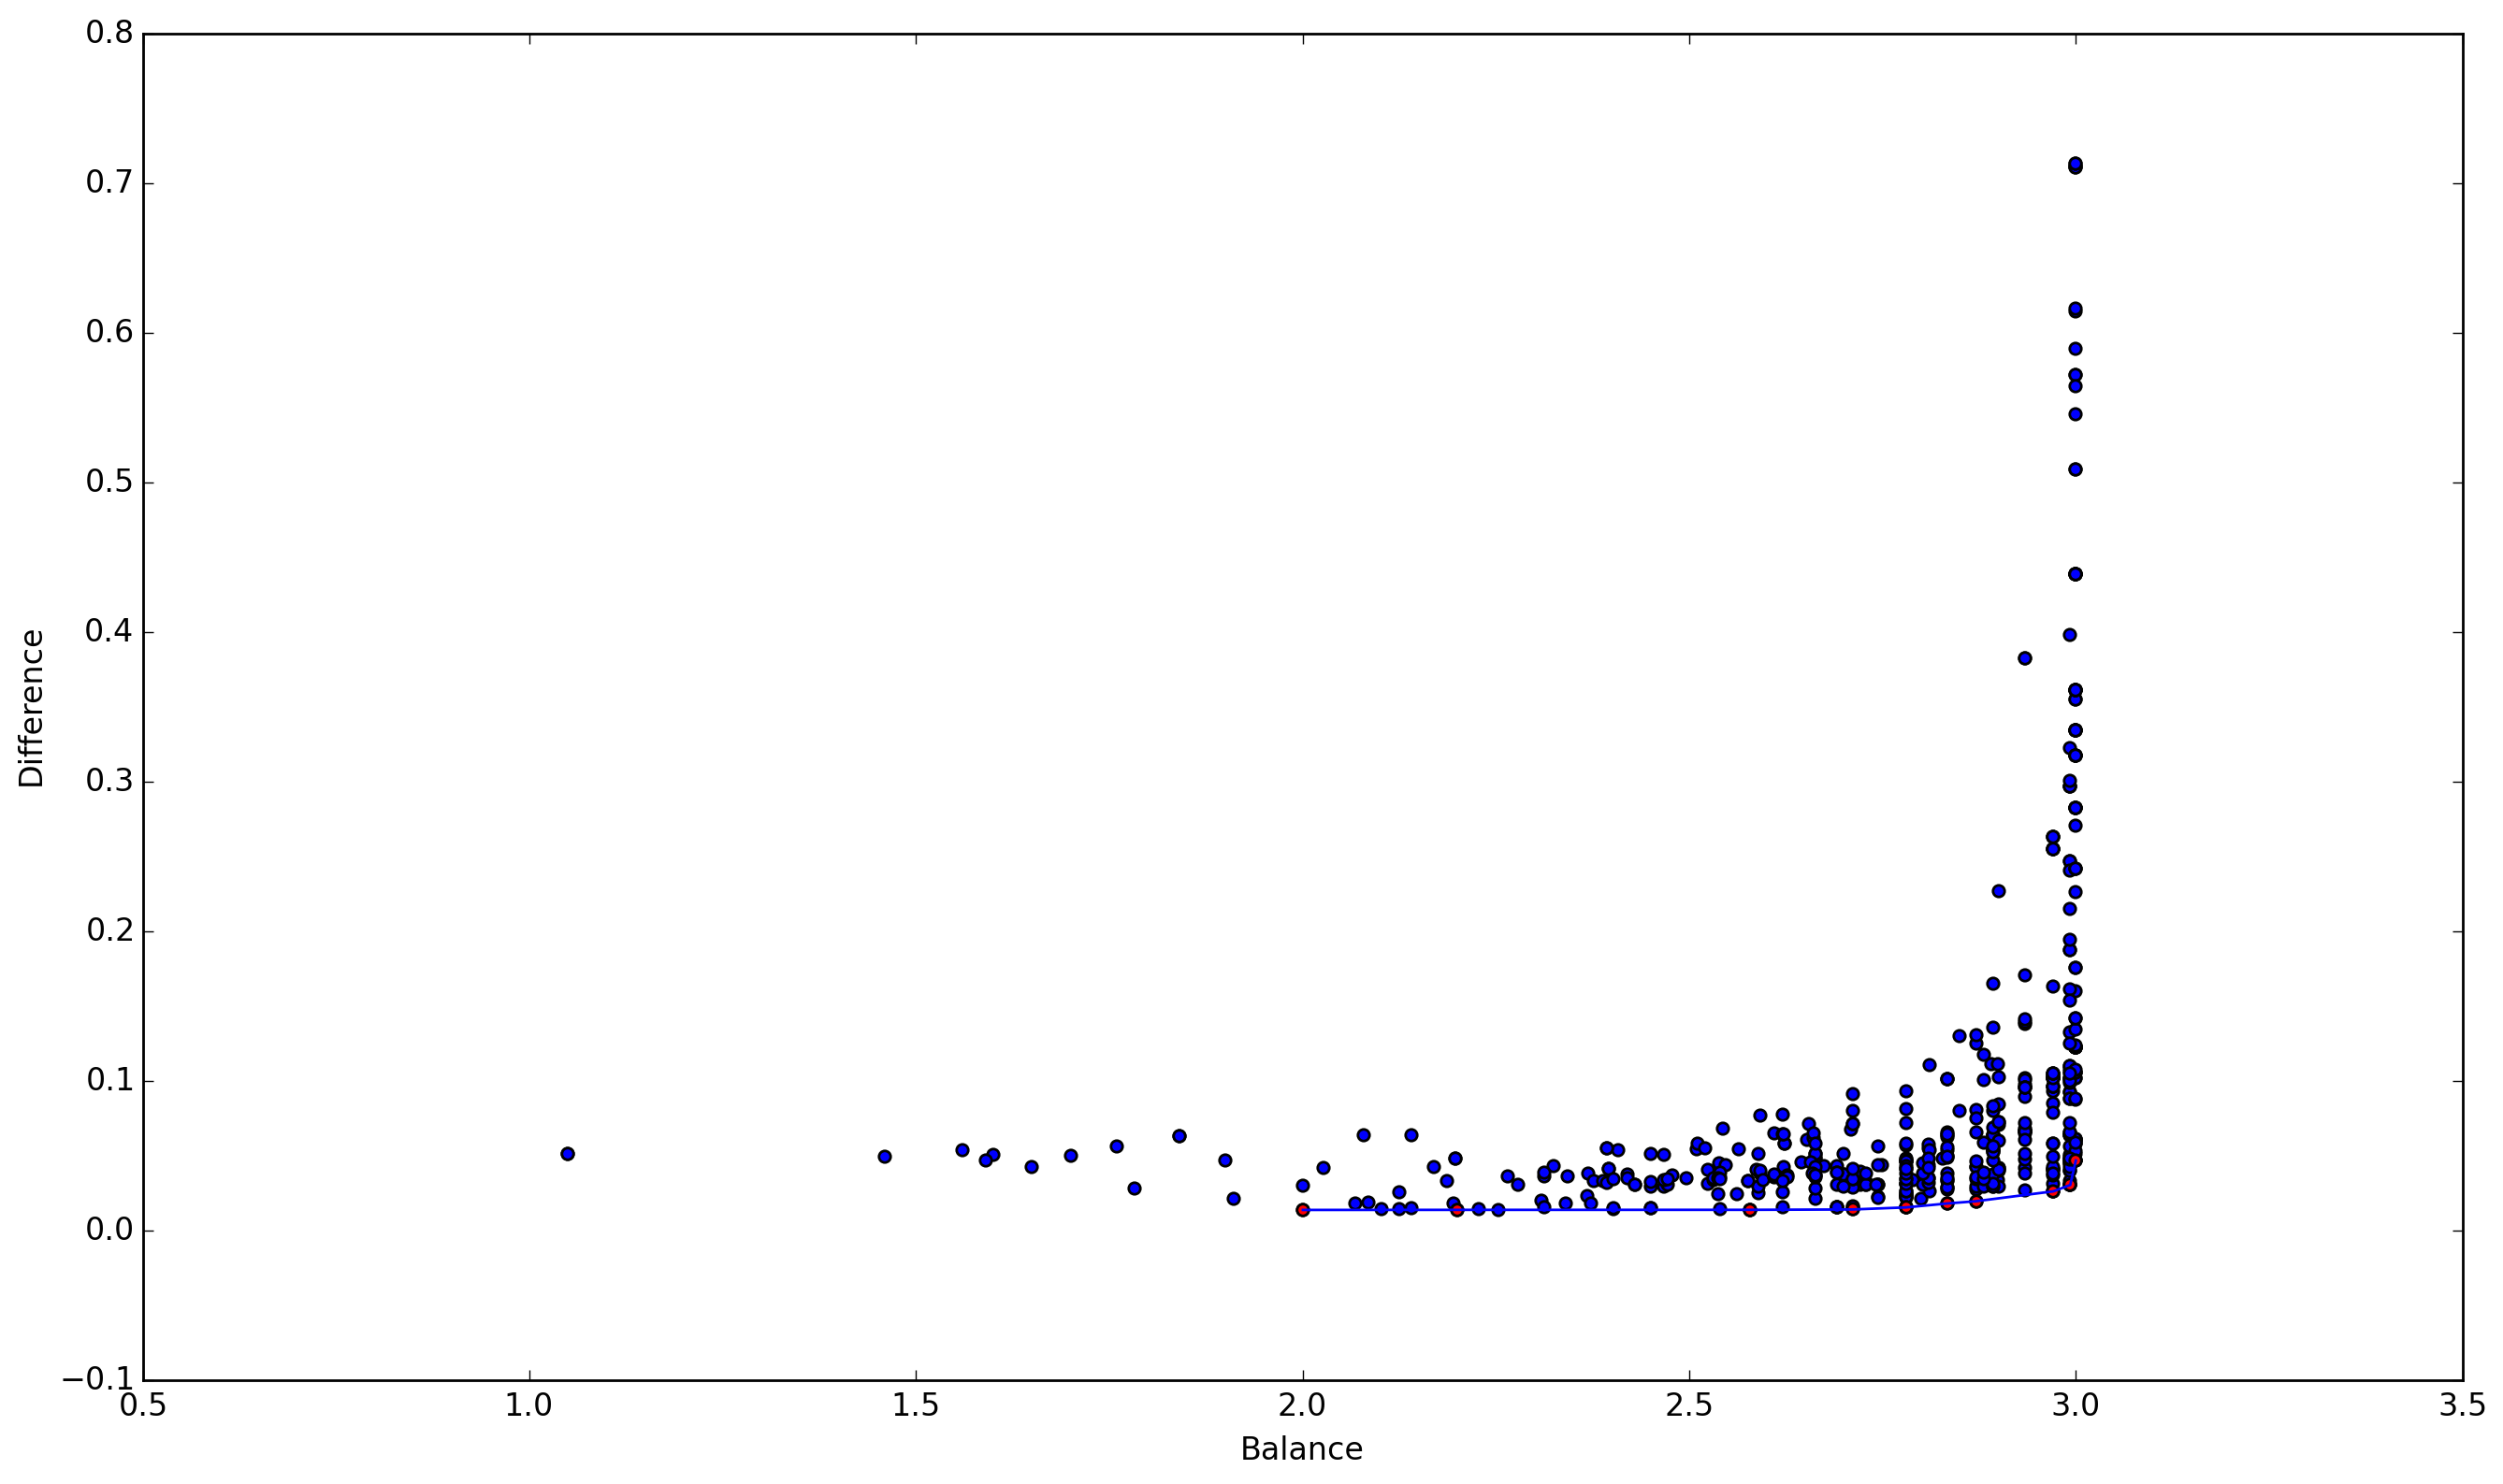
\includegraphics[width=1.0\textwidth]{pareto_single_weap}
\caption{pareto ottenuta con il bilanciamento dell'arma obiettivo}
\label{fig:pareto_single_weap}
\end{figure}

\subsection{Analisi delle soluzioni}
Nelle 10 prove effettuate dell'esperimento abbiamo ottenuto delle armi molto simili all'arma obiettivo e bilanciate.
Abbiamo quindi deciso di analizzare le caratteristiche principali delle armi ottenute nelle prove effettuate, in modo tale da valutare quali fossero le caratteristiche modificate dall'algoritmo che rendono l'arma obiettivo bilanciata.
Per visualizzare le caratteristiche emergenti di questi risultati, abbiamo raccolto le popolazioni finali ottenute nelle 10 prove, e le abbiamo sottoposte a un algoritmo di clustering.
Per il clustering abbiamo utilizzato l'algoritmo \emph{DBSCAN} \cite{dbscan:article} con $\epsilon = 0.05$ e $minPts = 5$, attraverso la libreria {P}ython \emph{scikit-learn} \cite{scikit-learn:article}.
Dopo aver effettuato il clustering abbiamo ottenuto 8 cluster data una popolazione di 500 individui, cioè la somma dei 50 individui finali ottenuti per ogni prova dell'esperimento effettuata.
Attraverso il clustering delle popolazioni finali andiamo ad analizzare quali sono effettivamente i parametri cambiati dall'algoritmo.
La figura \ref{fig:bar_single_weap} mostra per ogni parametro come si comportano in media le armi all'interno dei cluster ottenuti, indicati con una lettera (A-H), e inoltre mostriamo la media e la deviazione standard del bilanciamento e della distanza dall'arma obiettivo dei cluster.
\begin{figure}[htp]
\centering
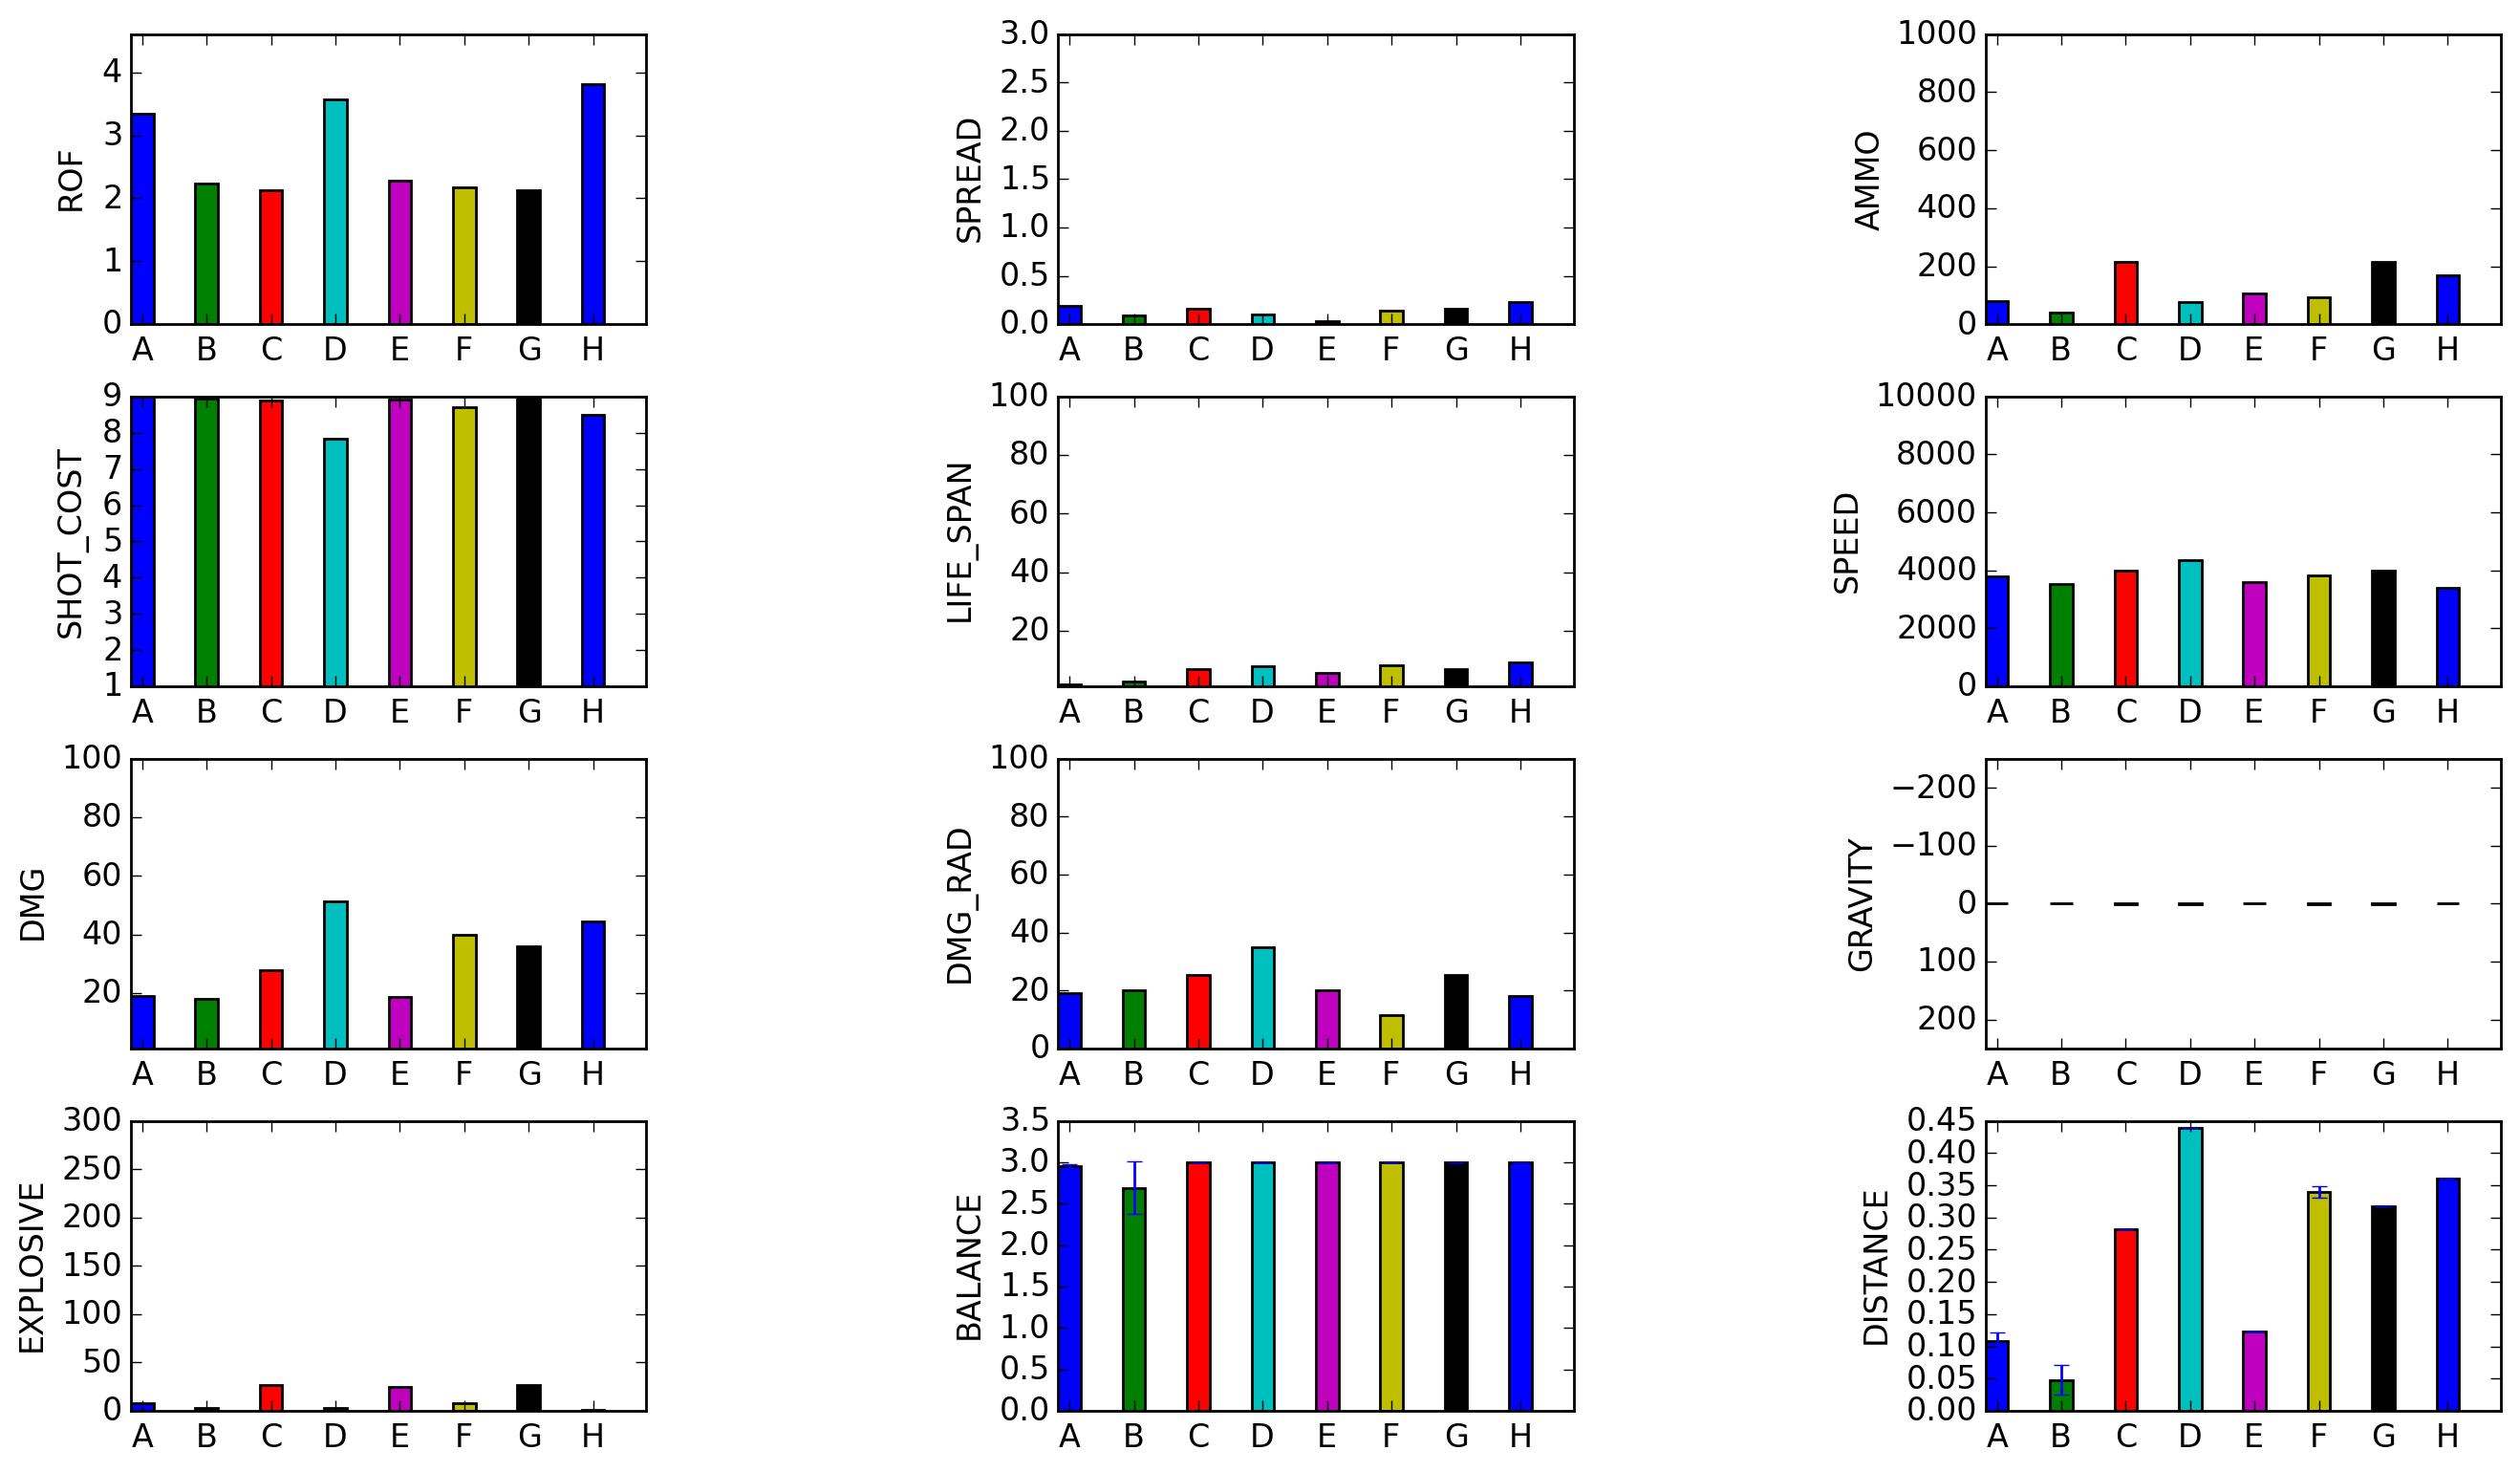
\includegraphics[width=1.2\textwidth, angle=90]{bar_single_weap}
\caption{Grafico a barre delle armi ottenute attraverso il \emph{tuning} dell'arma obiettivo}
\label{fig:bar_single_weap}
\end{figure}
Nella figura \ref{fig:bar_single_weap} possiamo vedere che il cluster B è praticamente uguale al \emph{Flak}, infatti la sua distanza media è al di sotto di $0.05$, mentre il bilanciamento è in media $2.69$, il più basso tra tutti i cluster ottenuti.
Questo cluster riunisce le armi che hanno un distanza euclidea minore a $0.1$ e come abbiamo detto precedentemente hanno un bilanciamento molto instabile, che diminuisce molto velocemente man mano che si avvicinano all'arma obiettivo.

In generale possiamo vedere che l'algoritmo ha modificato in particolare il rateo di fuoco delle armi, il numero di munizioni e il danno causato dai proiettili.
L'arma con il miglior \emph{trade-off} tra fitness e distanza è il cluster A: questo cluster mostra come le armi in media hanno incrementato il rateo di fuoco (\emph{Rate of Fire} e hanno una quantità di munizione leggermente più alta rispetto al \emph{Flak}. Queste armi riescono quindi a bilanciarsi rispetto al \emph{Rocket Launcher} grazie a un rateo di fuoco maggiorato e compensano il maggior numero di proiettili sparati per secondo con un numero di munizioni più alto.
Un altro cluster molto simile all'arma obiettivo e con un bilanciamento massimo è il cluster E: qui abbiamo un distanza media leggermente maggiore rispetto al cluster A, cioè $0.12$, e in questo caso le armi all'interno del cluster hanno reso praticamente nullo lo \emph{spread} dell'arma ($0.03$), hanno aumentato il numero di munizioni, pari a $105$, e infine ha aggiunto un piccolo raggio esplosivo ai proiettili.
Questa cluster riunisce delle armi che per bilanciare l'arma hanno puntato a massimizzare il danno per singolo colpo, in quanto uno \emph{spread} pari a $0.12$ aumenta la densità dei proiettili, e il numero maggiore di proiettili rende l'arma capace di colpire l'avversario con lunghe sequenze di spari.

\subsection{Esempi significativi}
Ora andremo ad analizzare nel dettaglio alcuni dei cluster migliori trovati nei risultati finali.
Nelle figure \ref{fig:rad_single_weap_1}, \ref{fig:rad_single_weap_2} e \ref{fig:rad_single_weap_3} mostriamo a sinistra il \emph{radar chart} dell'arma \emph{Flak} originale (nominata \emph{Target Weapon}), a destra il \emph{radar chart} della media dei parametri delle armi contenuti nel cluster preso in esame e infine due \emph{boxplot}, che mostrano come variano rispettivamente il bilanciamento e la distanza euclidea dall'arma obiettivo.
\begin{figure}[htp]
\centering
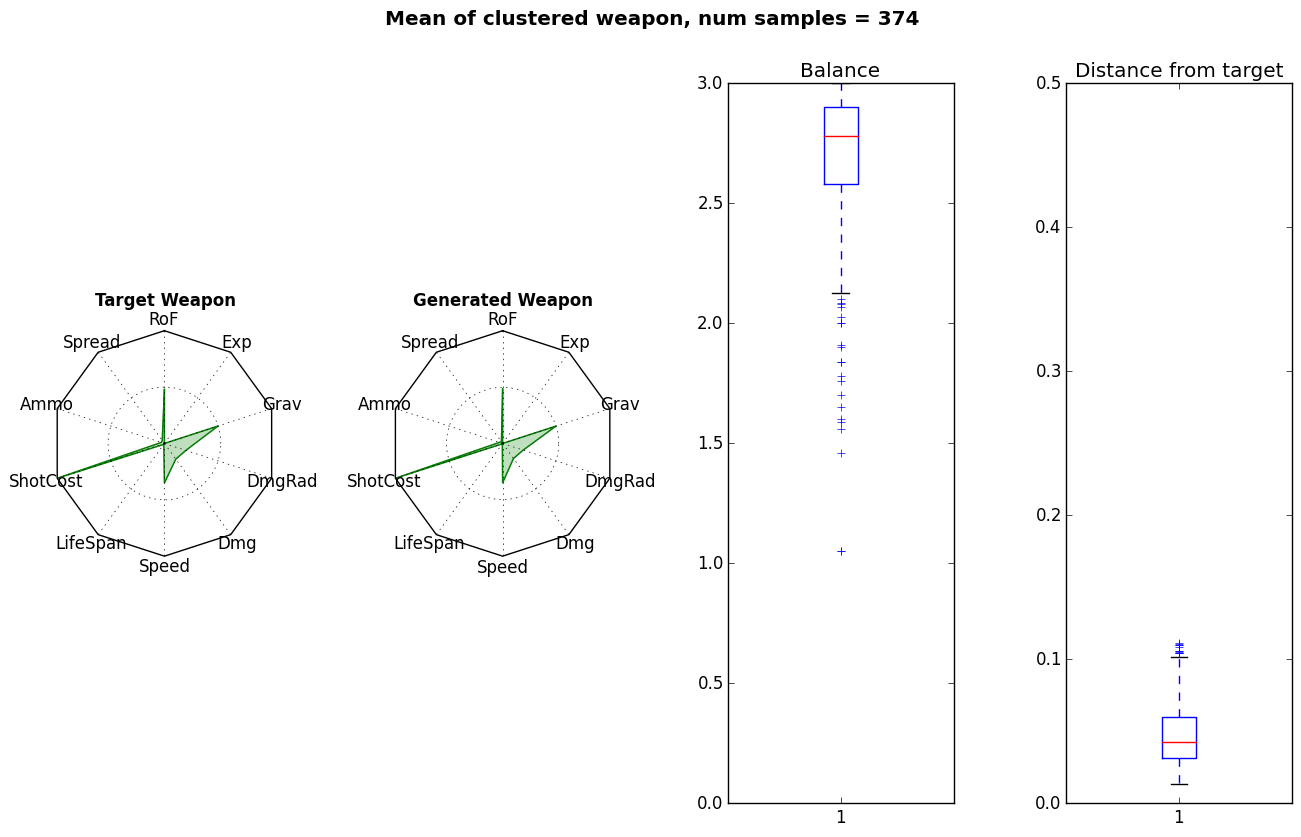
\includegraphics[width=1.0\textwidth]{rad_single_weap_1}
\caption{\emph{radar chart} della 1°  arma generata  attraverso il bilanciamento dell'arma obiettivo}
\label{fig:rad_single_weap_1}
\end{figure}
\begin{figure}[htp]
\centering
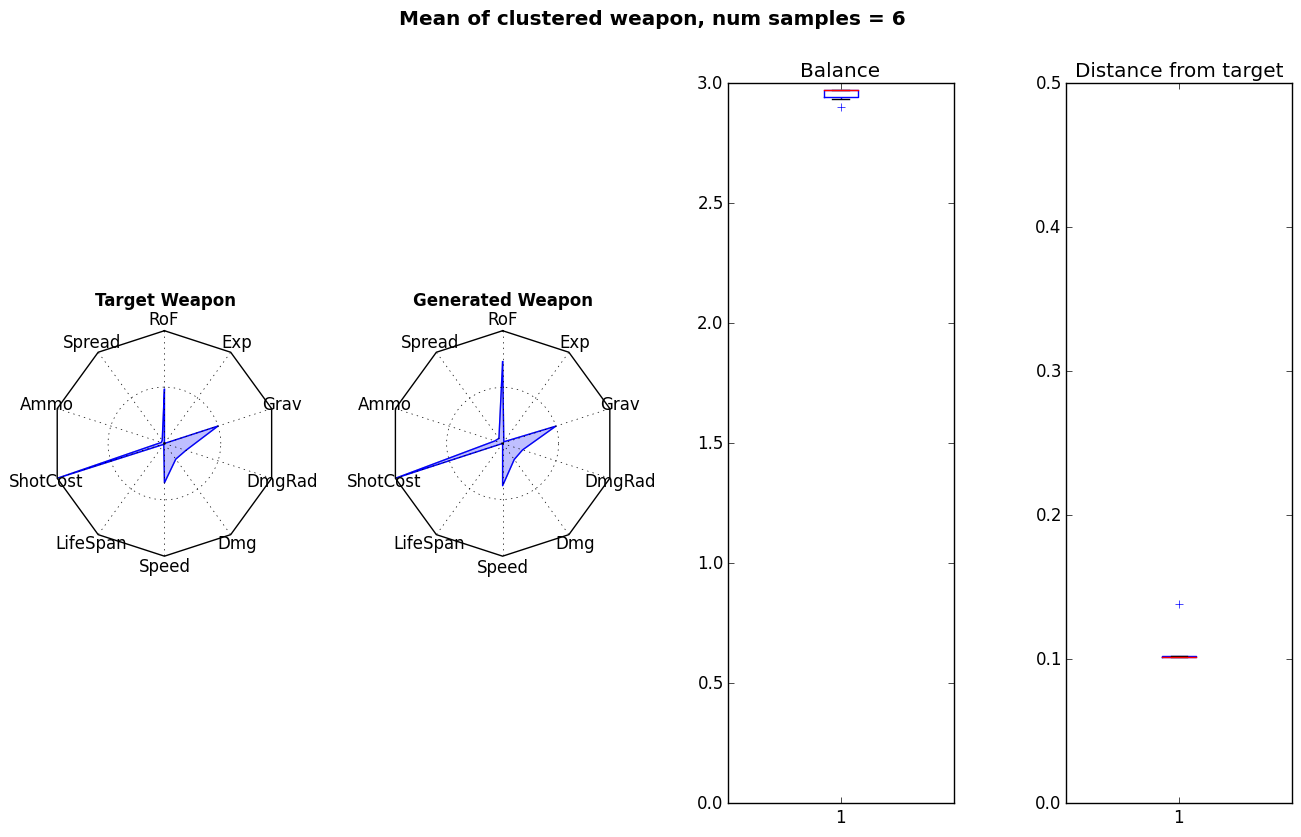
\includegraphics[width=1.0\textwidth]{rad_single_weap_2}
\caption{\emph{radar chart} della 2° arma generata  attraverso il bilanciamento dell'arma obiettivo}
\label{fig:rad_single_weap_2}
\end{figure}
\begin{figure}[htp]
\centering
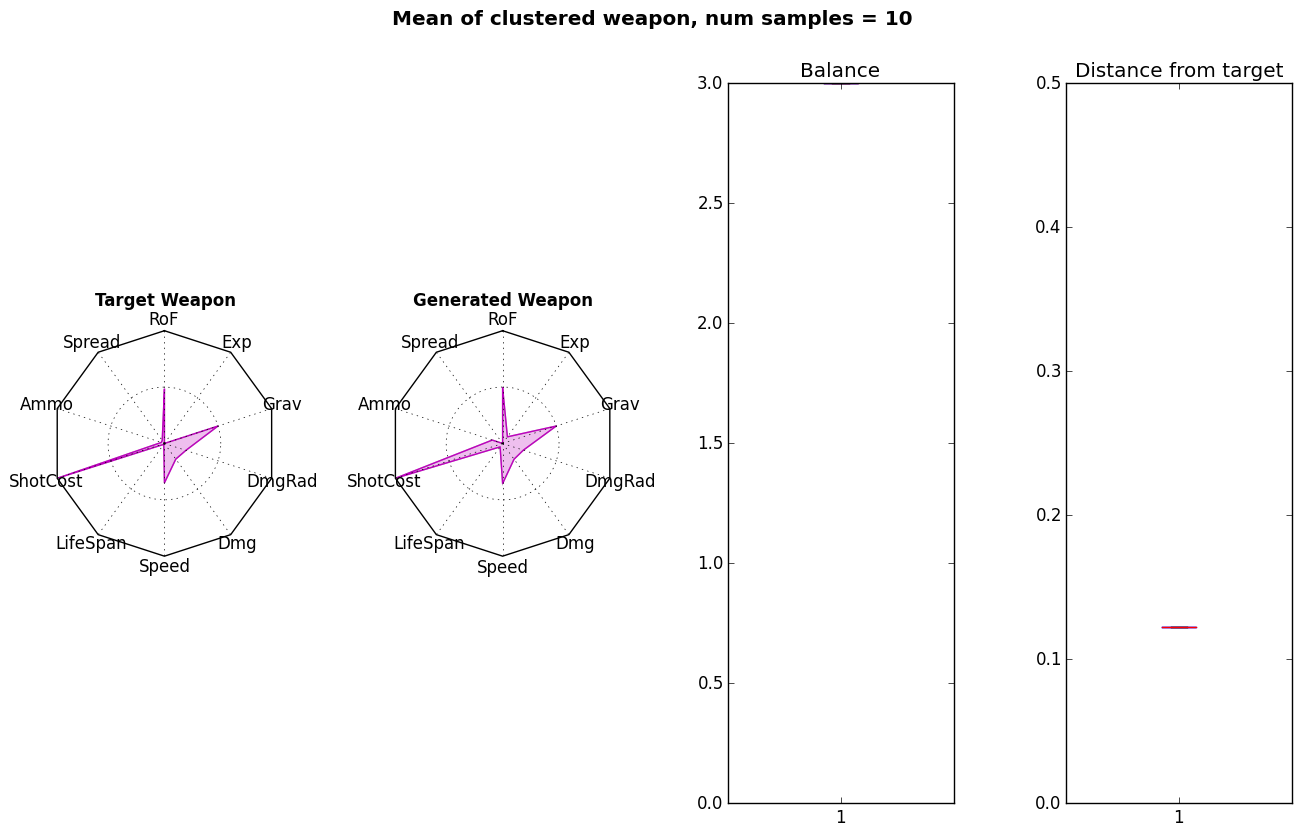
\includegraphics[width=1.0\textwidth]{rad_single_weap_3}
\caption{\emph{radar chart} della 3° arma generata  attraverso il bilanciamento dell'arma obiettivo}
\label{fig:rad_single_weap_3}
\end{figure}
Il primo cluster (vedi figura \ref{fig:rad_single_weap_1}) è il cluster che nella sottosezione precedente veniva indicato con la lettera B: come si vede il cluster è praticamente uguale all'arma obiettivo, ma abbiamo ottenuto una fitness molto variabile. Infatti, come abbiamo descritto precedentemente, può capitare che in alcune simulazioni le armi contenute in questo cluster siano di fatto equilibrate con il \emph{Rocket Launcher}, ma nel caso in cui il bot che possiede quest'ultima arma compia molti suicidi, la valutazione dell'equilibrio diventa molto variabile, come appunto è visibile dal \emph{boxplot} del bilanciamento.
Invece il cluster della figura \ref{fig:rad_single_weap_2} (cluster A nella precedente sottosezione) rende molto più stabile l'equilibrio tra le due armi, in virtù del rateo di fuoco più alto e di un numero di munizioni leggermente maggiorato. Infatti nel momento in cui la seconda arma riesce effettivamente a rendere equilibrato il match, diminuisce la probabilità di suicidio dovuto al \emph{Rocket Launcher},  in quanto il bot che la possiede non ha abbastanza tempo per sparare lunghe sequenze di colpi che alzano la probabilità di suicidio.
Anche il terzo cluster preso in analisi (\ref{fig:rad_single_weap_3}) (cluster E nella precedente sottosezione) mostra un bilanciamento molto più stabile, grazie a un numero di munizioni molto più alto, uno \emph{spread} praticamente nullo e un raggio esplosivo leggermente aumentato.
Questi esempi dimostrano la capacità dell'algoritmo di bilanciare anche finemente i parametri delle armi, in quanto è riuscito a generare un'insieme di armi molto simili all'arma obiettivo e capaci di modificare in modo puntuale alcuni parametri per rendere l'arma equilibrata.

\section{Validazione}
Nella Sezione \ref{sec:goal_score} abbiamo evidenziato come le simulazioni effettuate in UT3 abbiano un errore di valutazione del bilanciamento nel caso che il \emph{goal score} sia 20.
Per validare i risultati ottenuti dalle 10 prove effettuate in questo esperimento, abbiamo rivalutato il bilanciamento delle 10 popolazioni finali con un \emph{goal score} più ampio, pari a 40, il che ci permette di avere una stima più precisa del vero valore del bilanciamento delle armi generate.
Quindi abbiamo cambiato la configurazione delle simulazioni: il limite delle uccisioni totali per partita è stato cambiato con 40, e il tempo limite delle partite è stato impostato a 2400 secondi.

I risultati mostrano un errore medio, calcolato come differenza tra valutazione della fitness con \emph{goal score} pari 40 e \emph{goal score} pari a 20, di $0.088$ e una deviazione standard di $0.24$.
L'errore medio è relativamente piccolo, ma la deviazione standard invece è molto più grande. 
In questo esperimento i motivi sono due.
Il primo è il problema che abbiamo citato nella Sezione \ref{sec:error_single_obj}: ci sono delle simulazioni in cui l'intelligenza artificiale da dei risultati errati, dovuti alla velocità maggiorata a cui vengono eseguiti gli esperimenti.
Inoltre abbiamo un secondo problema, dovuto in questo caso ai proiettili con raggio esplosivo dell'arma fissa: il tempo maggiore concesso alle simulazioni di validazioni permette al bot che possiede l'arma fissa (il \emph{Rocket Launcher}) di avere una probabilità maggiore di compiere suicidi, in quanto avendo un tempo maggiore a disposizione, c'è una probabilità maggiore che il bot spari nelle sue vicinanze, suicidandosi. Questo crea un ulteriore rumore sulla valutazione della fitness, che come abbiamo detto nelle sezione precedente (Sezione \ref{sec:single_weap_result}), viene ridotto solo nel caso di armi equilibrate.
Per verificare che le armi più distanti dall'arma obiettivo hanno effettivamente un rumore minore rispetto alle armi con una distanza minore di $0.1$, che risultando meno equilibrate dovrebbero mostrare un errore più significativo, abbiamo ordinato gli individui delle popolazioni finali ottenute nei 10 esperimenti a seconda della loro distanza euclidea dall'arma \emph{Flak}.
La figura \ref{fig:error_vs_distance} mostra nel grafico superiore l'errore assoluto, calcolato come differenza tra bilanciamento ottenuto con \emph{goal score} pari a 40 e con \emph{goal score} pari a 20, delle armi ottenute nelle 10 prove ordinati da sinistra a destra per distanza crescente dall'arma obiettivo, e con il medesimo ordinamento mostriamo nel grafico inferiore la distanza degli individui dall'arma obiettivo.
Per rendere visivamente più chiari i risultati mostriamo la media mobile dell'errore assoluto nel grafico superiore e della distanza nel grafico inferiore.
Come si vede, l'errore aumenta proporzionalmente al diminuire della distanza: questo dimostra ulteriormente come effettivamente al di sotto della distanza limite di $0.1$ tra arma generata e l'arma \emph{Flak} il bilanciamento sia molto impreciso.

\begin{figure}[htp]
\centering
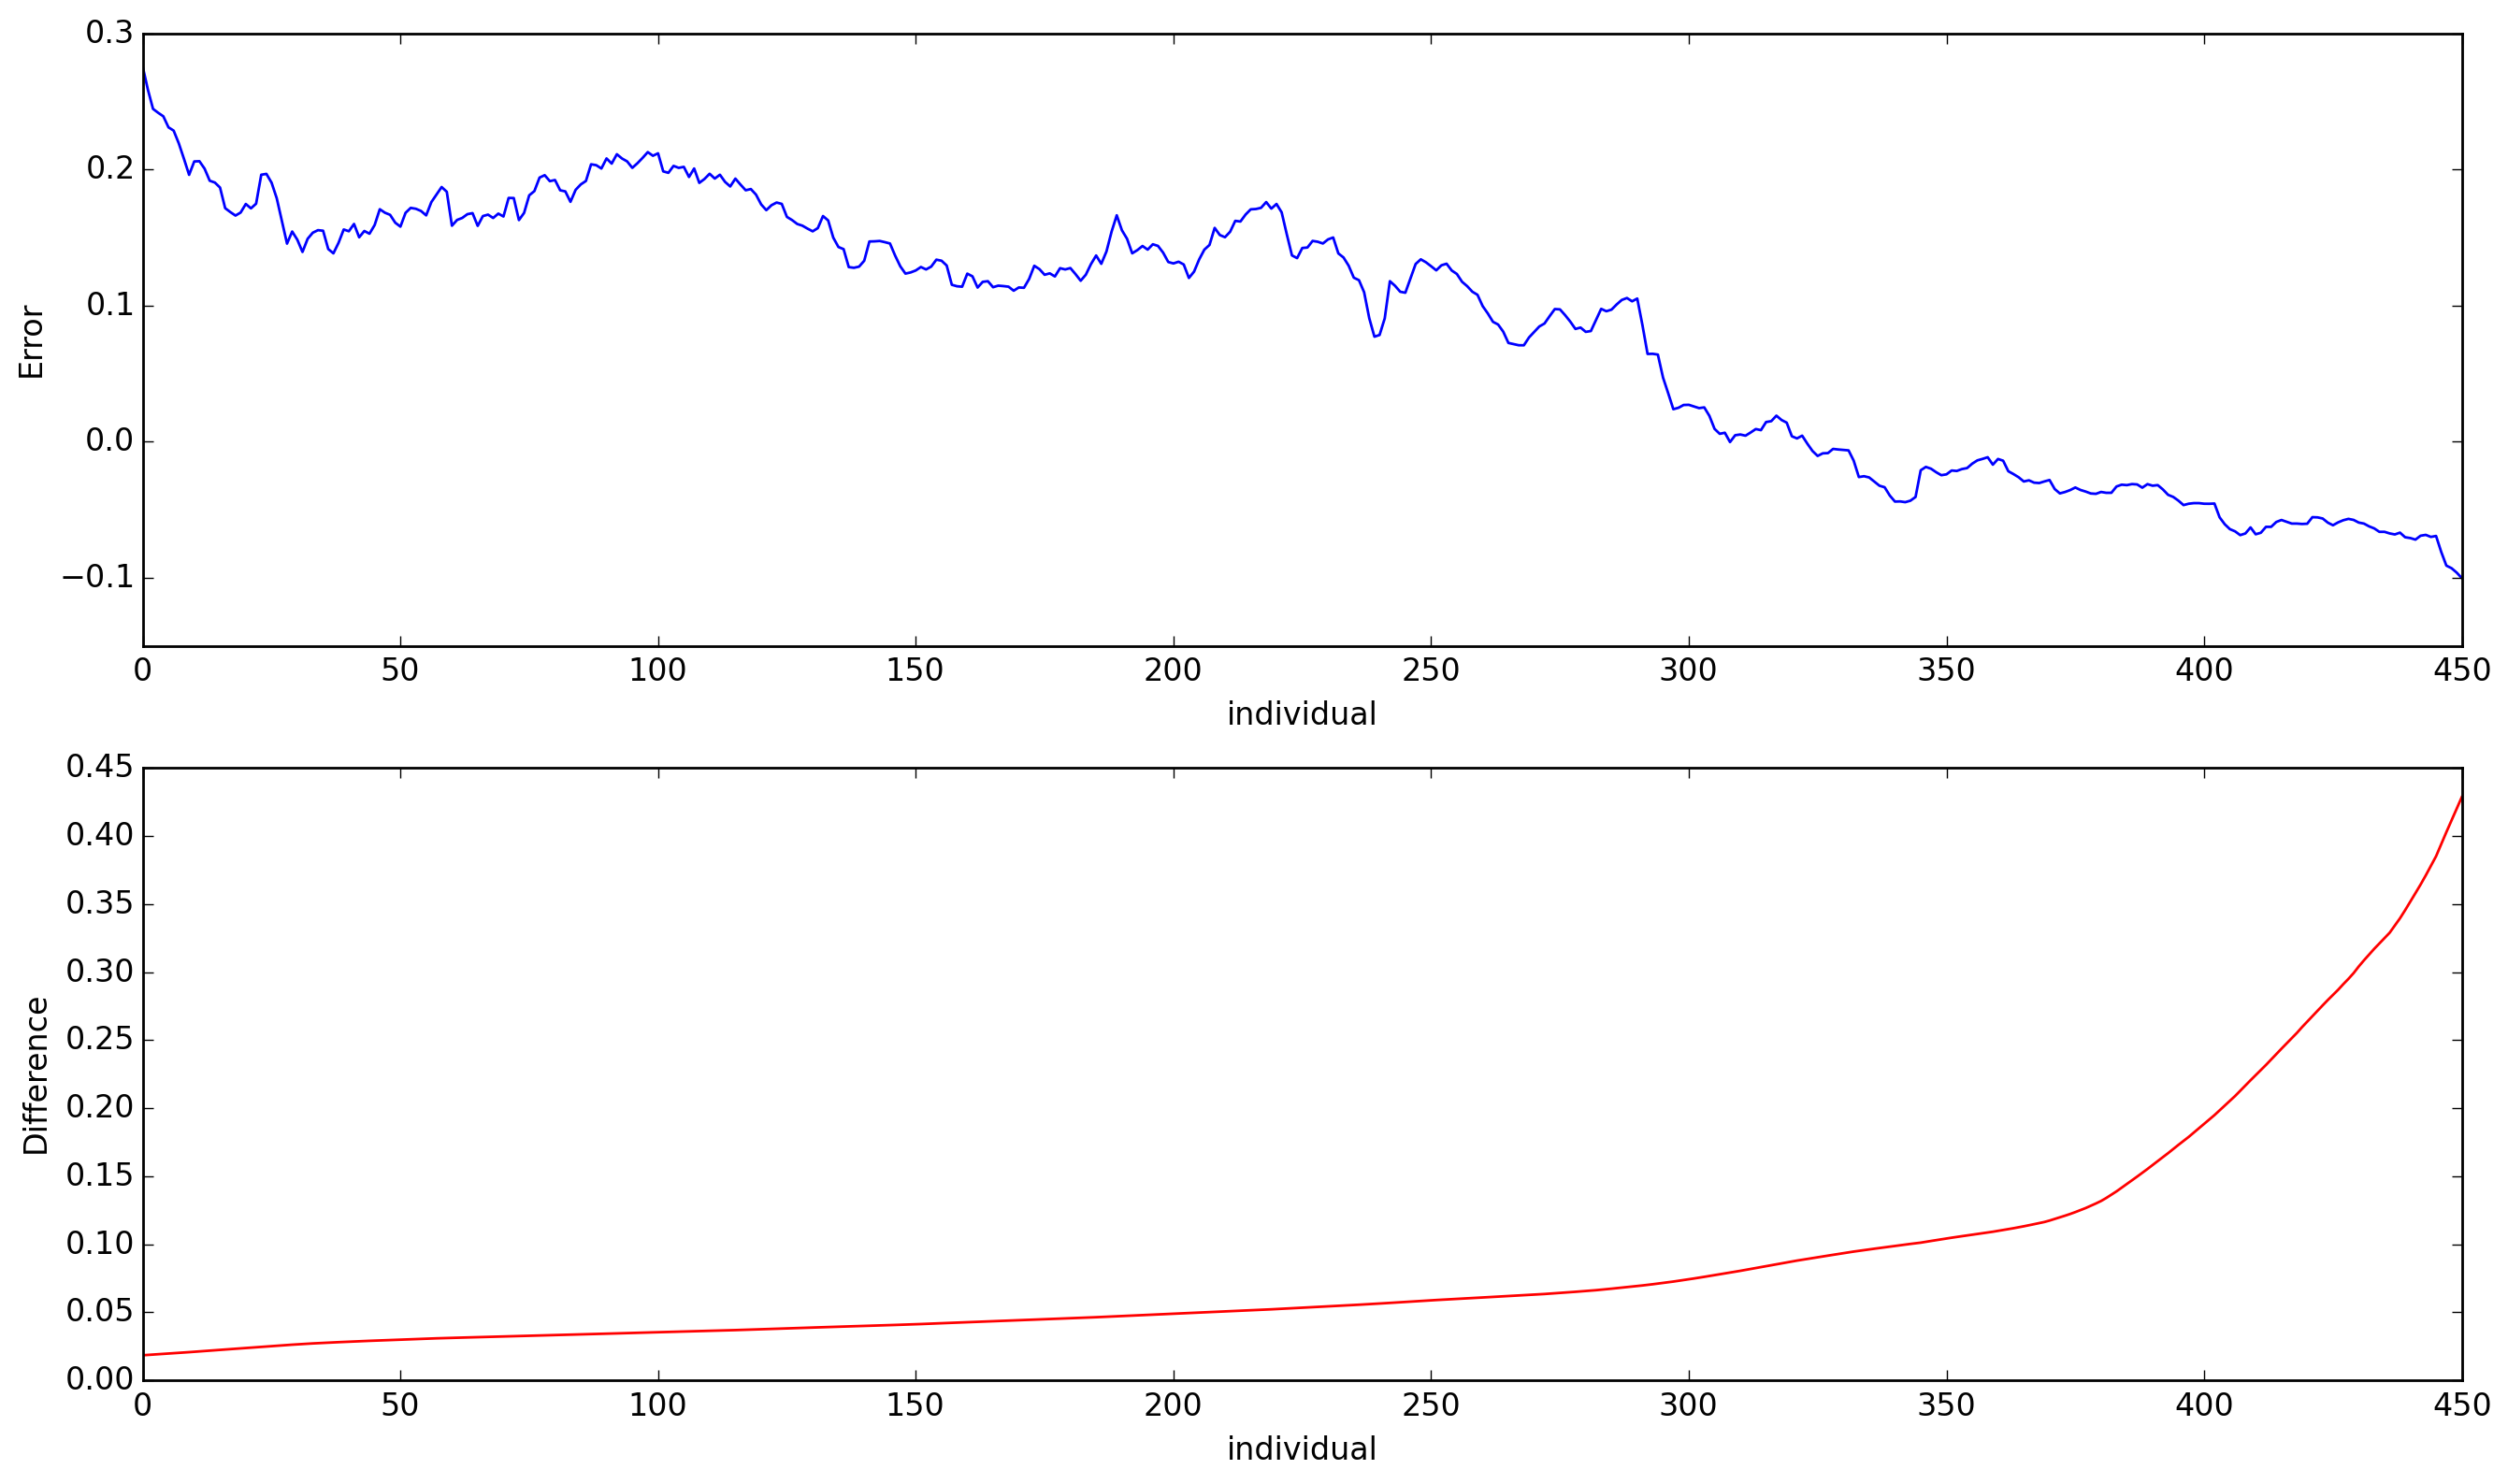
\includegraphics[width=1.0\textwidth]{error_vs_distance}
\caption{confronto tra media mobile dell'errore assoluto e media mobile della distanza euclidea dall'arma obiettivo}
\label{fig:error_vs_distance}
\end{figure}

Nella figura~\ref{fig:error_single_weap} visualizziamo nel dettaglio la media e la deviazione standard dell'errore (calcolato come differenza tra il bilanciamento ottenuto con \emph{goal score} pari a 40 e con \emph{goal score} pari a 20) per ogni popolazione finale ottenuta nei 10 esperimenti, e come si può vedere le considerazioni fatte precedentemente valgono anche per le singole popolazioni: qualitativamente possiamo notare un errore medio in generale molto piccolo e una deviazione standard sempre molto elevata rispetto all'errore medio.
\begin{figure}[htp]
\centering
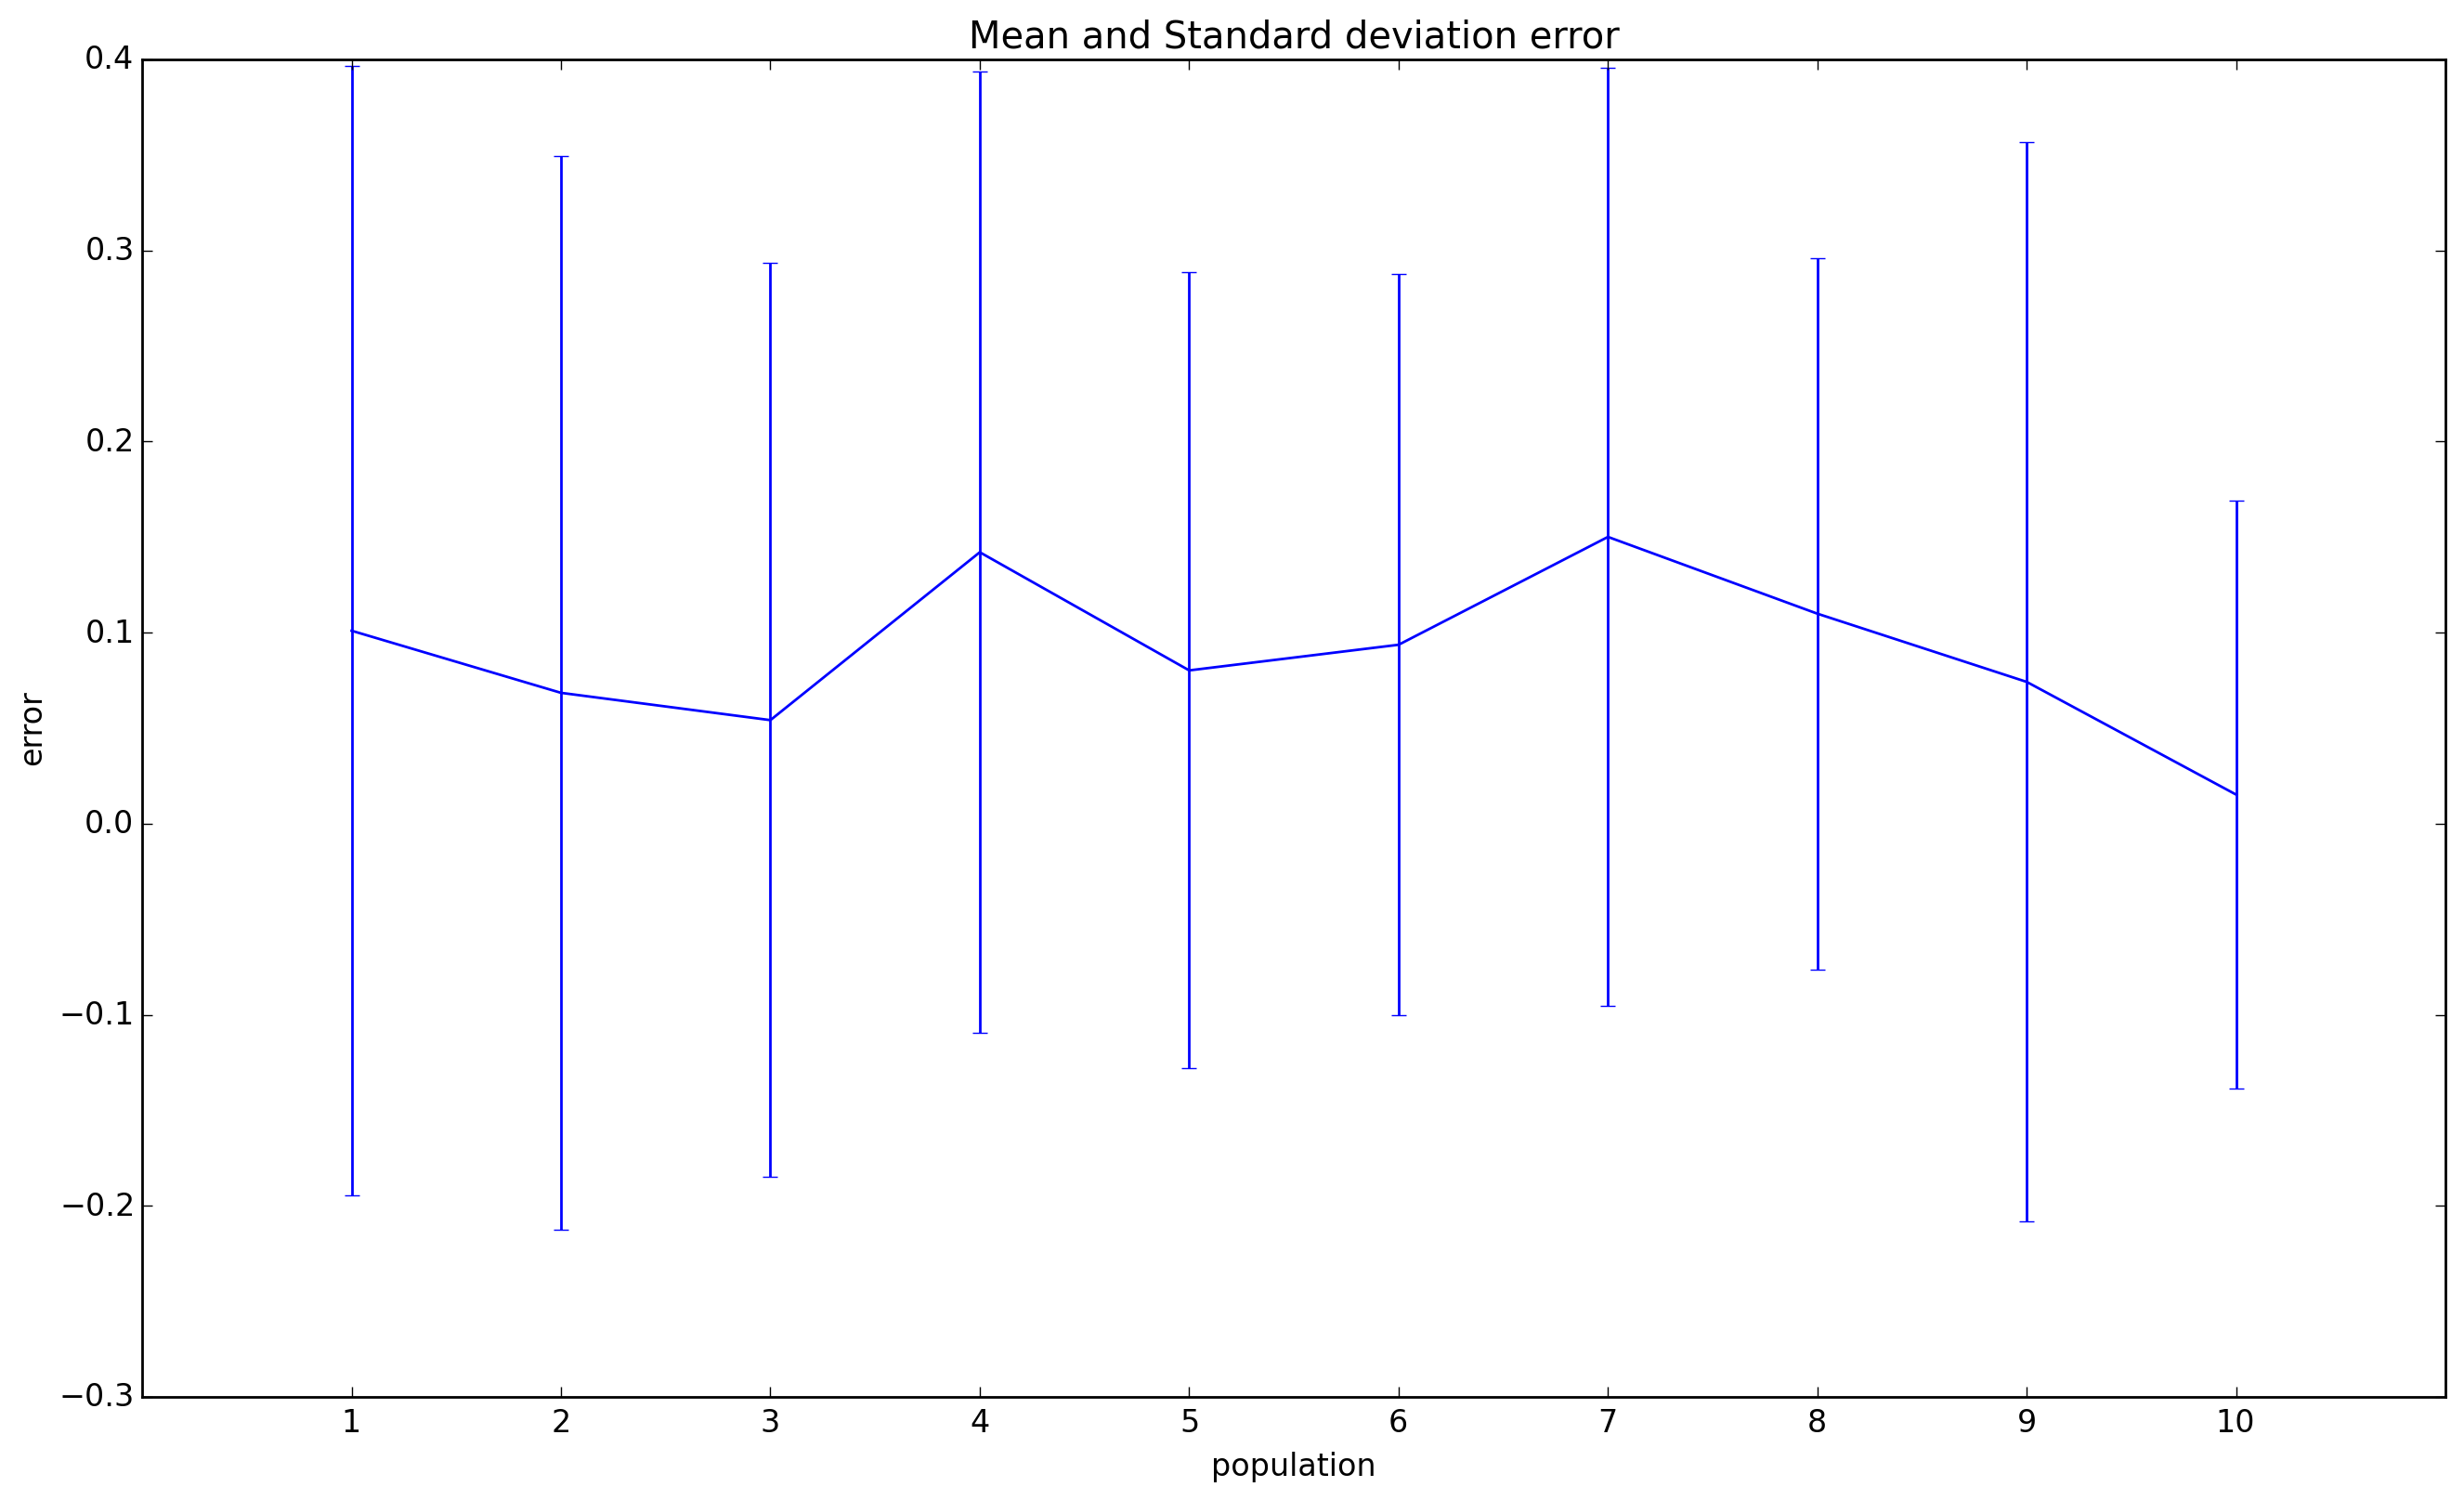
\includegraphics[width=1.0\textwidth]{error_single_weap}
\caption{media e deviazione standard dell'errore ottenuto dai risultati del bilanciamento dell'arma obiettivo}
\label{fig:error_single_weap}
\end{figure}

Per valutare i risultati ottenuti con un \emph{goal score} pari a 40 e fare un confronto qualitativo rispetto alle soluzioni ottenute con la valutazione con \emph{goal score} minore, mostriamo la pareto ottenuta dalle popolazioni finali ottenute con la nuova rivalutazione: la figura \ref{fig:pareto_single_weap_40} mostra il confronto tra distanza euclidea degli individui dall'arma obiettivo e la nuova valutazione del bilanciamento, dove i punti di colore blu sono le armi generate nelle 10 prove dell'esperimento e i punti di colore rosso sono la nuova pareto.
\begin{figure}[htp]
\centering
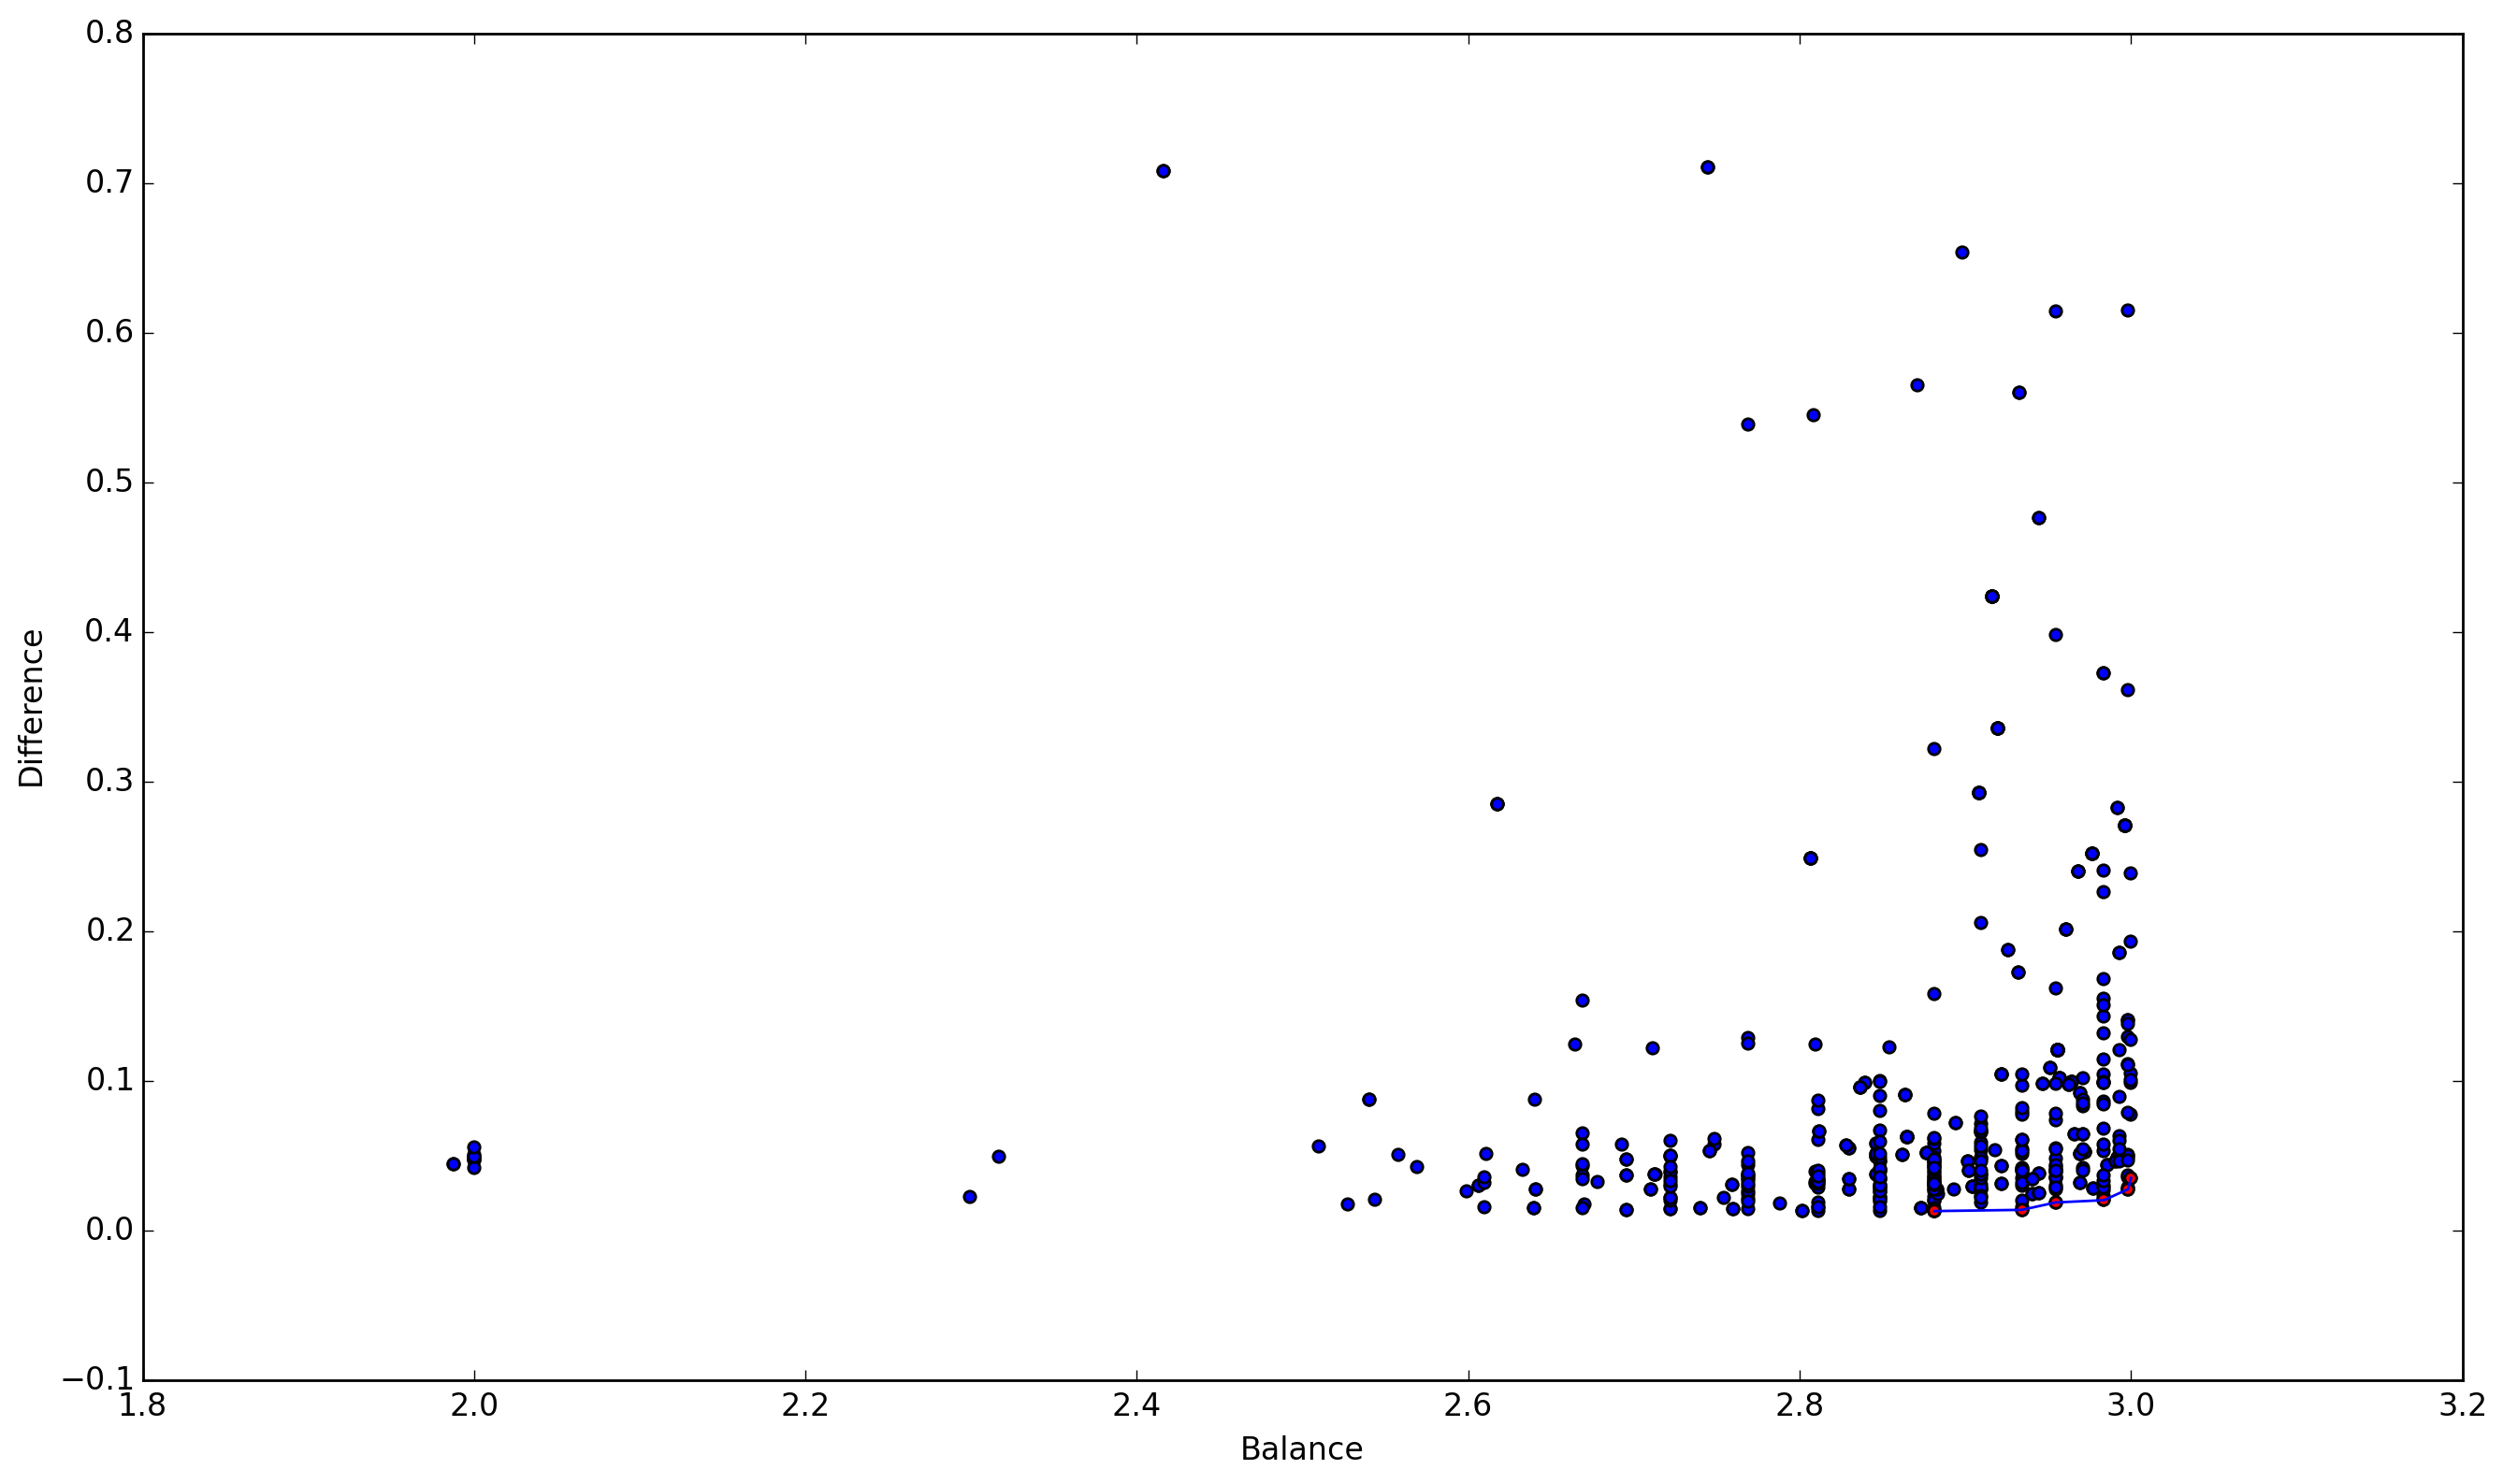
\includegraphics[width=1.0\textwidth]{pareto_single_weap_40}
\caption{pareto ottenuta con il bilanciamento dell'arma obiettivo nella validazione}
\label{fig:pareto_single_weap_40}
\end{figure}
Possiamo notare che abbiamo una valutazione più pessimistica delle armi generate, e che alcuni individui hanno una valutazione particolarmente differente, dovuta come abbiamo detto alle valutazione errate citate nella Sezione \ref{sec:error_single_obj}.
In generale possiamo concludere che le prestazioni degli individui sono molto simili alla valutazione con \emph{goal score} pari a 20: infatti possiamo notare che per gli individui con differenza dall'arma obiettivo minore di 0.1 gli individui hanno una valutazione decrescente del bilanciamento, esattamente come succedeva nella valutazione con \emph{goal score} minore.


\section{Sommario}
In questo capitolo ci siamo concentrati nel \emph{tuning} di un'arma obiettivo.
Nella Sezione 5.1 introduciamo le armi scelte per questo esperimento, cioè il \emph{Flak} e il \emph{Rocket Launcher}.
Nella Sezione 5.2 descriviamo i risultati ottenuti e mostriamo le armi migliori ottenute con questo esperimento.
Nella Sezione 5.3 infine andiamo a mostrare l'errore ottenuto rivalutando i risultati ottenuti con un \emph{goal score} pari a 40.

\chapter{Generazione di armi bilanciate con vincoli}
Ci siamo chiesti se fosse possibile vincolare la generazione delle armi con alcuni obiettivi aggiuntivi, con lo scopo di generare armi con determinati requisiti di gameplay.
Lo scenario applicativo di questi esperimenti è fornire uno strumento che generi coppie di armi equilibrate secondo alcuni vincoli decisi dal game designer.
Per mostrare le potenzialità di questo tipo di generazione abbiamo scelto tre vincoli, anche se potrebbero essere facilmente estesi con altri obiettivi secondari:
\begin{itemize}
\item Distanza media dei colpi ottenuti con l'arma, che chiameremo \emph{distanza media};
\item Tempo medio che trascorre tra quando un proiettile viene sparato e quando colpisce l'avversario, abbreviato con \emph{Hit Time};
\item Sequenza media di uccisioni effettuati con l'arma senza essere uccisi dall'avversario, che chiameremo \emph{Kill Streak}.
\end{itemize}

Inizialmente andremo a descrivere il design sperimentale in cui si svolgono questi esperimenti.
Successivamente andremo ad analizzare i risultati ottenuti in tre diversi esperimenti effettuati scegliendo diverse combinazioni dei tre obiettivi secondari:
\begin{itemize}
\item Distanza media dei colpi per la prima arma e \emph{Kill Streak} per la seconda;
\item \emph{Hit time} per la prima arma e \emph{Kill Streak} per la seconda;
\item \emph{Hit time} per la prima arma e distanza media dei colpi per la seconda;
\end{itemize}
Infine andremo a validare i risultati ottenuti nei tre esperimenti mediante una rivalutazione del bilanciamento delle armi ottenute con delle simulazioni più precise.

\section{Design Sperimentale}
In questa sezione andremo a descrivere l'algoritmo genetico scelto per gli esperimenti di questo capitolo e i parametri sperimentali utilizzati; successivamente andremo a descrivere come formalizziamo attraverso la funzione di fitness gli obiettivi secondari scelti per questi esperimenti, cioè la distanza media, l'\emph{Hit Time} e la \emph{Kill Streak}.

\subsection{Algoritmo e Parametri Sperimentali}
L'algoritmo utilizzato in questi esperimenti è un algoritmo multiobiettivo, dove come primo obiettivo abbiamo il bilanciamento, mentre i due obiettivi secondari dipendono dai vincoli scelti per l'esperimento.
Abbiamo scelto di effettuare tre esperimenti:
\begin{enumerate}
\item Massimizzazione del bilanciamento, della distanza media della prima arma e della \emph{Kill Streak} per la seconda;
\item Massimizzazione del bilanciamento , dello \emph{Hit time} per la prima arma e della \emph{Kill Streak} per la seconda;
\item Massimizzazione del bilanciamento , dello \emph{Hit time} per la prima arma e distanza media dei colpi per la seconda;
\end{enumerate}
L'implementazione dell'algoritmo scelta per questi esperimenti è l'\emph{NSGA-II} \cite{nsga2:article}, attraverso la libreria {P}ython  DEAP\cite{deap:article}.
Gli operatori genetici scelti per questi esperimenti sono i seguenti:  per il crossover abbiamo scelto il \emph{simulated binary crossover} con probabilità 0.9; per la mutazione abbiamo scelto la \emph{simulated binary mutation} con probabilità 0.05; e infine come selezione abbiamo scelto la \emph{tournament selection} a due individui.
Come abbiamo descritto nella Sezione \ref{sec:nsga2}, con questo algoritmo abbiamo un forte elitismo, per cui abbiamo deciso di utilizzare una probabilità di crossover molto più alta rispetto a quella usata nel Capitolo 4.

La \emph{rappresentazione} consiste in un vettore di 20 elementi: i primi 10 rappresentano i parametri della prima arma, mentre i successivi 10 rappresentano la seconda arma, quindi abbiamo nuovamente un \emph{encoding diretto}.
Dopo alcune valutazioni, abbiamo deciso di effettuare 50 generazioni per singola prova degli esperimenti, con una popolazione composta da 100 individui.
La simulazione avviene sulla mappa \emph{DM-Biohazard}, con un \emph{goal score} pari a 20 uccisioni totali e un tempo limite di 1200 secondi.
Le singole prove degli esperimenti hanno avuto una durata media di 16 ore.

\subsection{Funzione di Fitness}
Negli esperimenti descritti in questo capitolo possiamo assegnare degli obiettivi da massimizzare oltre al bilanciamento: la distanza media, lo \emph{Hit Time} e la \emph{Kill Streak}.
Uno di questi tre obiettivi può essere assegnato a un'arma della coppia da generare,  in modo tale che l'algoritmo genetico cerchi di massimizzare l'obiettivo indicato per l'arma selezionata.
Per formalizzare questi tre obiettivi abbiamo utilizzato tre funzioni aggiuntive, descritte nella tabella \ref{tab:vincoli}.
\begin{table}[htp]
\caption{Vincoli sulle armi}
\label{tab:vincoli}
\centering
	\begin{tabularx}{\textwidth}{lXr}
	\toprule
	Funzione & Descrizione & Unità Di Misura\\
	\midrule
	Distanza media & Media delle distanze coperte dai proiettili tra quando vengono sparati e quando colpiscono l'avversario & $UU$\\
	\midrule
	Hit Time & Media dei tempi medi impiegati dai proiettili tra quando vengono sparati e quando colpiscono l'avversario & $secondi$ \\
	\midrule
	Kill Streak & Media delle sequenze di uccisioni compiute con l'arma senza essere uccisi dall'avversario & $uccisioni$ \\
	\bottomrule
	\end{tabularx}
\end{table}
La distanza media ha come limite inferiore 0 UU, e non ha un limite superiore; lo \emph{Hit Time} ha come limite inferiore 0 secondi e ha come limite superiore la durata massima della partita, nel nostro caso 1200 secondi;
infine la \emph{Kill Streak} ha come limite inferiore 0 uccisioni e come limite superiore il \emph{goal score} cioè 20 uccisioni.
Queste tre funzioni sono calcolate dal server alla fine della simulazione in base ai dati raccolti dalla partita e vengono inviati al client per tutte e due le armi inviate, oltre al numero di uccisioni e suicidi dei due bot, come descritto nella Sezione \ref{sec:simulation}.
Quindi lato client, l'algoritmo estrae dai dati ricevuti solo quelli relativi all'obiettivo selezionato per l'arma, e ne assegna una fitness pari esattamente al valore della statistica ricevuta dal server.
Riassumendo la fitness di una coppia di armi è così composta:
\begin{itemize}
\item Bilanciamento --  $f_e + f_g + f_s$
\item Obiettivo selezionato per la prima arma
\item Obiettivo selezionato per la seconda arma
\end{itemize}
Il calcolo del bilanciamento è il medesimo descritto nella Sezione \ref{subsec:fitness}.

Ora andremo a descrivere nel dettaglio i risultati ottenuti dai singoli esperimenti effettuati.

\section{Massimizzazione distanza media e \emph{Kill Streak}}
\label{sec:dist_kill}

In questo esperimento andiamo a massimizzare la distanza media della prima arma e la \emph{Kill Streak} della seconda. 
Abbiamo condotto 10 prove di questo esperimento e abbiamo raccolto i risultat irelativi alla fitness delle armi generate e le popolazioni finali ottenute nelle prove.
Ora andremo a descrivere le prestazioni dell'algoritmo dal punto di vista delle tre funzioni da massimizzare, cioè bilanciamento, distanza media della prima arma e \emph{Kill Streak} della seconda.
Quindi andiamo ad analizzare i risultati ottenuti usano un algoritmo di clustering sugli individui ottenuti dalle 10 prove effettuate, in modo tale da analizzarne le caratteristiche emergenti per ogni obiettivo.
Successivamente mostreremo tre esempi principali, che massimizzano rispettivamente uno dei tre obiettivi di questo esperimento.
Infine ad analizzare l'errore con un validazione compiuta con delle valutazioni più precise dei risultati attraverso delle simulazioni con \emph{goal score} pari a 40.

\subsection{Analisi delle prestazioni}

Dopo aver effettuato 10 prove dell'esperimento abbiamo raccolto i dati relativi alla fitness delle popolazioni finali ottenute dalle prove effettuate.
Nella figura \ref{fig:pareto_dist_kill} mostriamo tre grafici: nel primo in alto a sinistra mostriamo i dati delle fitness relativi al confronto tra distanza media della prima arma e bilanciamento, in alto a destra mostriamo i dati relativi al confronto tra \emph{Kill Streak} della seconda arma e bilanciamento e infine nell'ultimo grafico mostriamo il confronto tra distanza media della prima arma e \emph{Kill Streak} della seconda. Con i punti blu indichiamo gli individui presenti nelle popolazioni finali, mentre con i punti rossi le pareto di ogni combinazione dei tre obiettivi.
Se prendiamo il primo grafico, si può notare come le armi riescano a essere bilanciate solo fino ad una distanza massima intorno ai 1000 UU, dopodiché abbiamo un decadimento molto veloce del bilanciamento, in quanto l'arma che massimizza la distanza diventa troppo avvantaggiata rispetto alla seconda arma, in quanto una distanza media troppo lunga permette di colpire senza essere mai colpiti. 
Se invece andiamo ad analizzare il grafico \emph{Kill Streak}-Bilanciamento possiamo notare che riusciamo ad ottenere armi bilanciate fino a una \emph{Kill Streak} massima di 10, cioè la metà del \emph{goal score}: questo è ragionevole in quanto nel caso un'arma riesca ad ottenere una sequenza di uccisioni maggiore a 10, è sicuramente più avvantaggiata rispetto all'arma avversaria, in quanto per avere armi bilanciate il massimo delle uccisioni concesse a un'arma è esattamente la metà del \emph{goal score}.
Per quanto riguarda invece l'ultimo grafico, notiamo che la \emph{Kill Streak} e la distanza media dei colpi sono due obiettivi conflittuali: quando la distanza media ha il suo massimo, 2500 $UU$, la \emph{Kill Streak} è intorno a valori tra 0 e 5, mentre quando la \emph{Kill Streak} è al suo massimo, cioè 19 uccisioni, la distanza media della prima arma diminuisce fino a 1000 $UU$. Questo è sempre dovuto al bilanciamento delle due armi: quando la distanza media dei colpi della prima arma è molto alto ($2500$ $UU$) la prima arma è in netto vantaggio sulla seconda, e questa non ha la possibilità di fare \emph{kill streak} che superino le 5 uccisioni; mentre quando la \emph{kill streak} della seconda arma è vicina al suo limite teorico (19 uccisioni) vuol dire che il bot con la prima arma non riesce a fare nemmeno una uccisione in quanto la seconda arma è così forte che non permette di ottenere nessuna uccisione a lunga distanza.

\begin{figure}[tp]
\centering
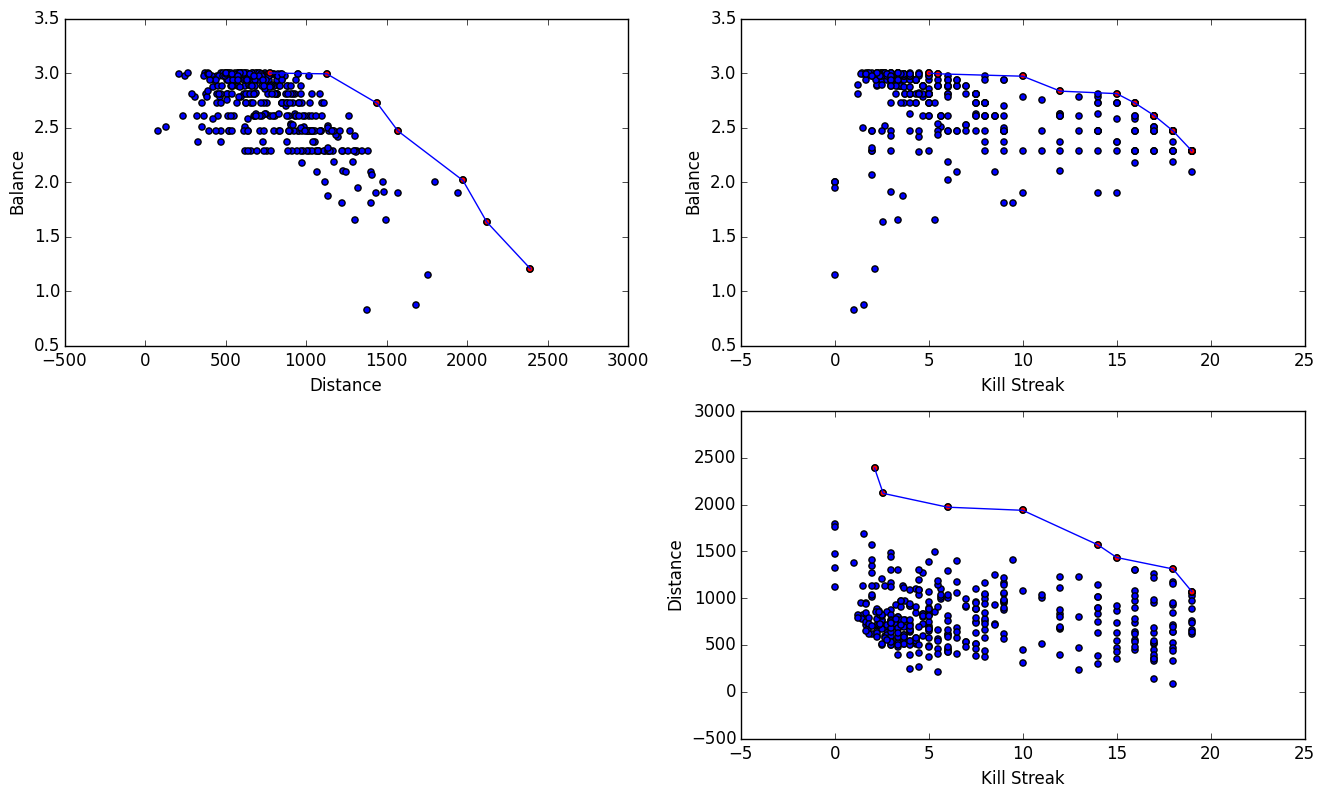
\includegraphics[width=1.0\textwidth]{pareto_dist_kill}
\caption{pareto ottenuto con il GA multiobiettivo (bilanciamento, distanza media e \emph{Kill Streak})}
\label{fig:pareto_dist_kill}
\end{figure}

\subsection{Analisi delle soluzioni}
Come abbiamo visto, nelle 10 prove effettuate siamo riusciti ad ottenere armi che riescono a massimizzare uno dei tre obiettivi, sebbene nessuna coppia di armi è riuscita ad ottenere dei buoni risultati in tutti e tre gli obiettivi contemporaneamente.
Per analizzare le caratteristiche trovate dall'algoritmo che riescono a massimizzare i tre obiettivi abbiamo sottoposto le popolazioni finali ottenute dalle 10 prove a un algoritmo di \emph{clustering}.
Per il clustering abbiamo utilizzato \emph{DBSCAN} con $\epsilon = 0.2$ e un numero minimo di punti per cluster pari a 5: abbiamo ottenuto 37 cluster da una popolazione finale composta da 1000 individui.
Nella figura \ref{fig:bar_dist_kill} mostriamo come si comportano in media le coppie di armi contenute nei cluster ottenuti (indicati da una lettera) per ogni parametro dell'arma. Per ogni cluster abbiamo due barre: la prima rappresenta il valore del parametro per la prima arma e la seconda rappresenta il valore del parametro per la seconda arma. In più ci sono tre grafici a barre che rappresentano rispettivamente la media e la varianza del bilanciamento, la media e la varianza della distanza media della prima arma e la media e la varianza della \emph{kill streak} della seconda arma.
Il primo aspetto che notiamo è che il parametro \emph{explosive} non è più così contenuto in tutte le armi come nell'esperimento della Sezione 4.1: questo è ragionevole in quanto la prima arma massimizzando la distanza può permettersi di avere dei raggi esplosivi più alti, in quanto massimizzando la distanza dei colpi ha una minore probabilità di fare danno al giocatore che la possiede, come per esempio nel cluster H.
La seconda arma cerca di aumentare il danno per singolo colpo, in modo tale da ottenere \emph{kill streak} più lunghe possibili. L'algoritmo ha quindi cercato di ottenere una combinazione di parametri per ottenere questo risultato e in un caso (cluster C) l'algoritmo ha cercato di aumentare il raggio esplosivo della seconda arma, con il risultato di ottenere delle valutazioni sul bilanciamento molto basse a causa dei suicidi, come si vede dalla valutazione del bilanciamento per il cluster C.
\'E possibile notare come la prima arma che compare nelle coppie abbiano un \emph{Rate of fire} in media molto basso: il primo motivo è che l'algoritmo cerca di bilanciare l'arma rallentando il suo rateo di fuoco, in modo tale che non sia avvantaggiato dal suo raggio di fuoco maggiore rispetto alla seconda arma; il secondo è che il bot avendo più tempo per mirare riesce a ottenere dei colpi con precisione maggiore (a meno di uno \emph{spread} molto alto), e quindi riesce a coprire distanze maggiori., come per esempio nel cluster C.
Al contrario la seconda arma delle coppie ha sempre un rateo di fuoco in media molto alto: questo perché dovendo massimizzare la \emph{Kill Streak} dell'arma, l'algoritmo ha cercato di aumentare il danno per secondo, in modo da ottenere sequenze di uccisioni più lunghe possibili.
Lo \emph{spread} della prima arma è spesso (tranne nel cluster F) minore di 0.5: il motivo è che dovendo massimizzare la distanza dei colpi abbiamo bisogno di armi precise, e quindi la soluzione è minimizzare lo \emph{spread} dei colpi.
Sempre per la prima arma abbiamo in media un rapporto tra gravità e velocità spesso molto piccolo, specie nei casi in cui otteniamo le distanze più alte, come nel cluster C: questo perché una gravità troppo alta rispetto alla velocità provocherebbe delle traiettorie non lineari, che pregiudicano la massimizzazione della distanza media dei colpi.
Per il seconda arma non abbiamo particolari sequenze di parametri che identificano un'arma che massimizzi la \emph{kill streak}: in generale possiamo dire che queste armi cercano di ottenere delle combinazioni di parametri che incrementano il danno per secondo, per esempio aumentando il danno e lo \emph{shotcost} per poter ottenere una uccisione per colpo, come nel caso del cluster H.

\begin{figure}[tp]
\centering
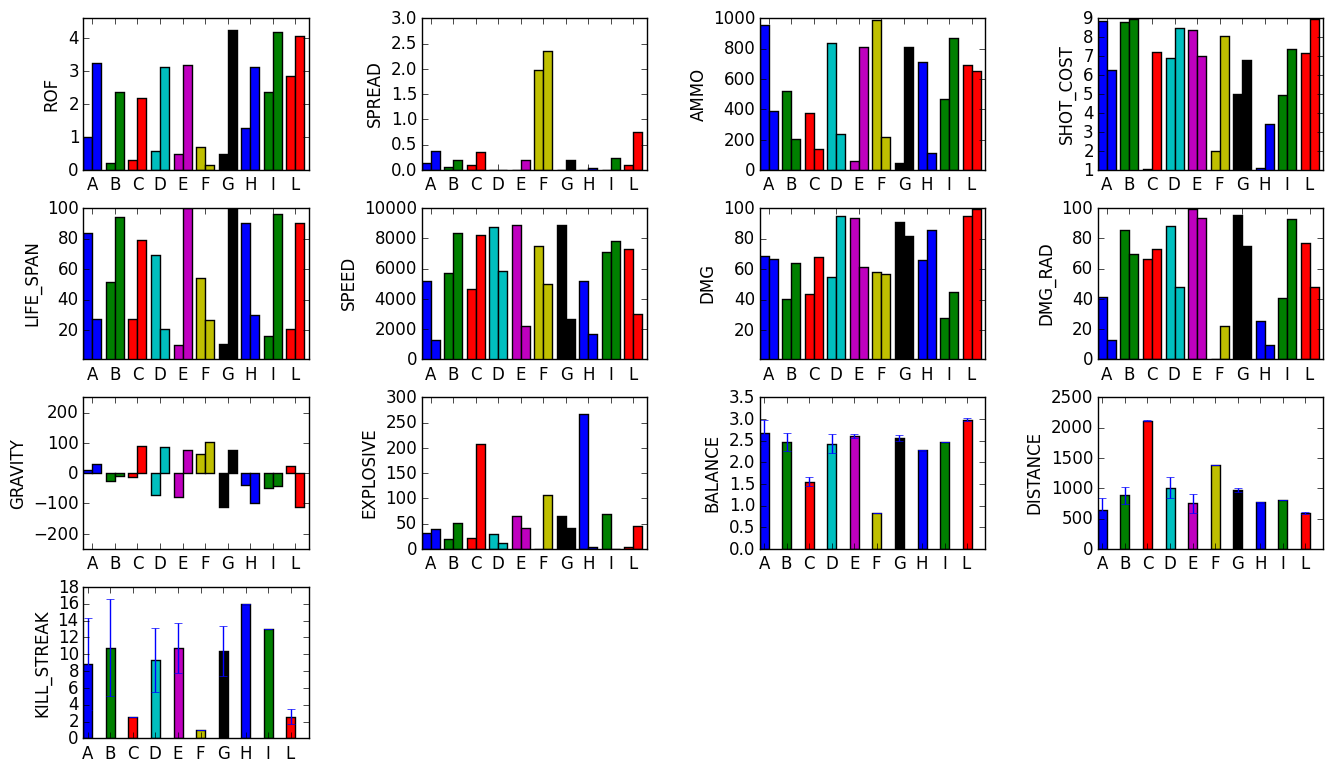
\includegraphics[width=1.2\textwidth, angle=90]{bar_dist_kill}
\caption{Grafico a barre delle armi ottenute attraverso \emph{clustering} con il GA multiobiettivo (bilanciamento, distanza media e \emph{Kill Streak}) }
\label{fig:bar_dist_kill}
\end{figure}


\subsection{Esempi significativi}
Ora andremo a descrivere nel dettaglio tre cluster che riescono a massimizzare uno dei tre obiettivi di questo esperimento.
Nelle figure \ref{fig:rad_dist_kill_1}, \ref{fig:rad_dist_kill_2} e \ref{fig:rad_dist_kill_3} mostriamo i \emph{radar chart} dei parametri delle due armi generate ottenute come media delle armi contenute nel cluster, e inoltre mostriamo tre \emph{boxplot} dei risultati ottenute dalle armi contenute nel cluster rispetto alle tre funzioni obiettivo.

Nella figura \ref{fig:rad_dist_kill_1} notiamo che in questo cluster la distanza media dei colpi ottenuta dalla prima arma è molto alta, 2212 UU. In questo cluster l'algoritmo ha massimizzato il raggio di danno dei proiettili e minimizzato gravità, \emph{shotcost} e \emph{spread} per essere più precisa possibile;  inoltre il rateo di fuoco è piuttosto basso. Queste caratteristiche ricordano molto i fucili da cecchino che possiamo trovare nei FPS. La seconda arma è notevolmente sbilanciata rispetto alla prima, come è possibile vedere dal \emph{boxplot} del bilanciamento, in quanto il raggio di fuoco della prima arma non permette al bot che possiede la seconda arma di avvicinarsi e quindi non gli permette di ottenere alcuna uccisione.
\begin{figure}[tp]
\centering
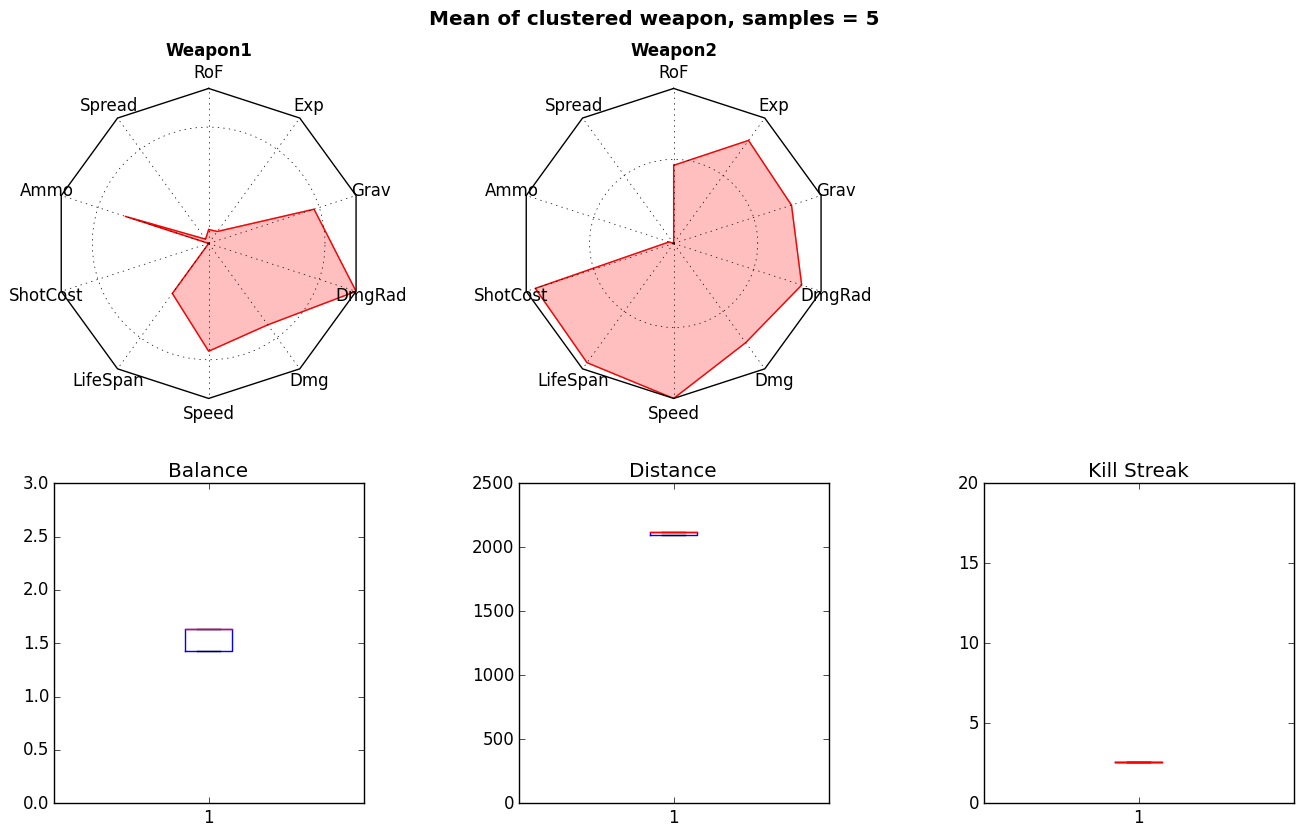
\includegraphics[width=1.0\textwidth]{rad_dist_kill_1}
\caption{\emph{radar chart} della 1°  arma generata con GA multiobiettivo (bilanciamento, distanza media e \emph{Kill Streak})}
\label{fig:rad_dist_kill_1}
\end{figure}
Nel secondo esempio preso in esame nella figura \ref{fig:rad_dist_kill_2}, la seconda arma ha ottenuto delle \emph{kill streak} in media molto alte, pari a 15. Come possiamo vedere, la \emph{kill streak} è un valore molto variabile, in quanto si basa su un numero di dati più basso rispetto al primo obiettivo. Infatti la \emph{kill streak} si basa unicamente sulla media di sequenze di uccisioni, le quali al massimo sono 20, mentre il primo obiettivo si basa su tutti i colpi sparati che colpiscono l'avversario nell'intera durata della partita.
L'algoritmo, in questo caso, ha massimizzato il \emph{rate of fire} e il raggio di danno dei proiettili. Queste combinazione permette di avere la maggiore probabilità di ottenere lunghe sequenze di uccisioni, grazie al danno notevole provocato per singolo sparo combinato all'altissimo rateo d fuoco, che viene parzialmente compensato dallo \emph{spread}.
\begin{figure}[tp]
\centering
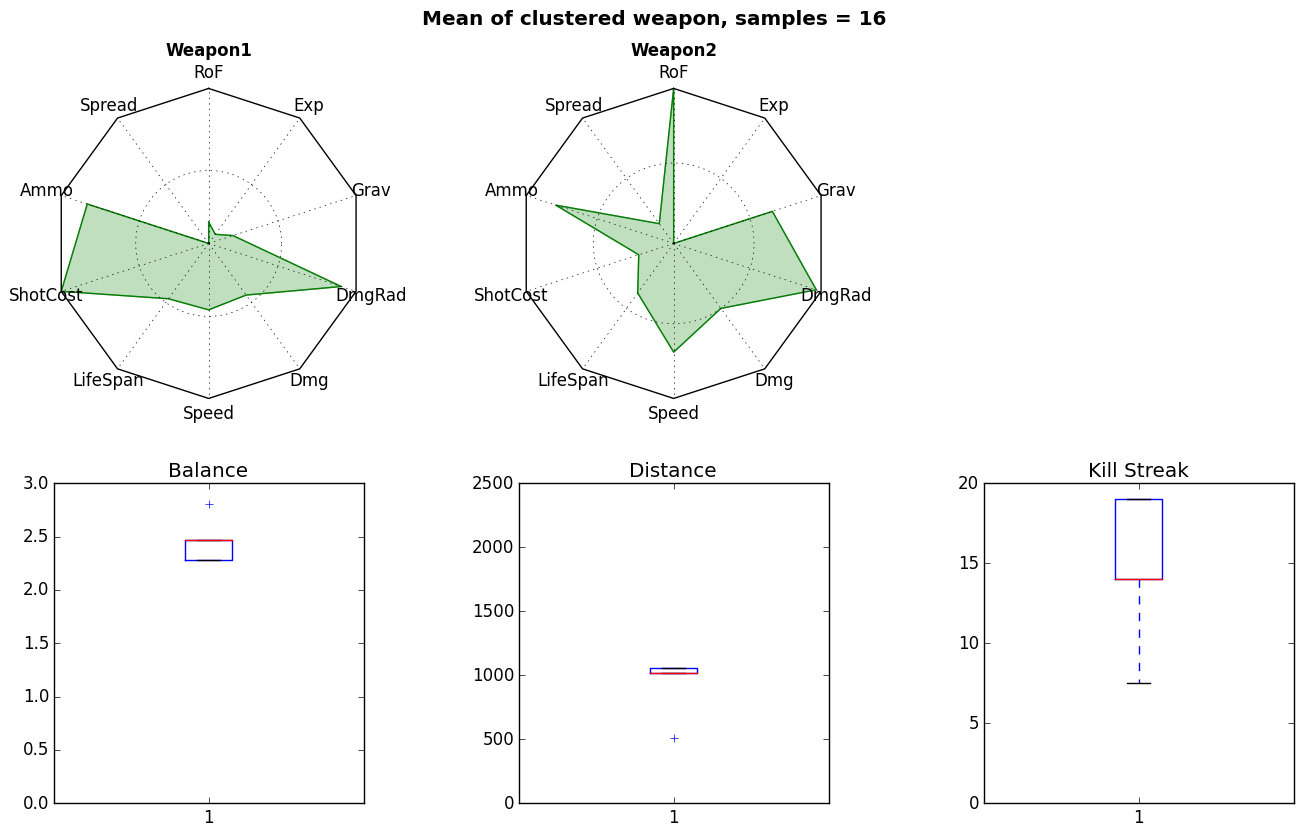
\includegraphics[width=1.0\textwidth]{rad_dist_kill_2}
\caption{\emph{radar chart} della 2°  arma generata con GA multiobiettivo (bilanciamento, distanza media e \emph{Kill Streak})}
\label{fig:rad_dist_kill_2}
\end{figure}
Infine se andiamo a scegliere una coppia di armi equilibrate, le armi hanno dei grossi limiti rispetto ai loro obiettivi secondari: la prima arma ha in media una distanza pari a 764 UU mentre la seconda arma riesce a totalizzare una \emph{Kill Streak} solo pari a 1.5. Il bilanciamento si basa sul limitare la loro efficienza rispetto ai loro obiettivi secondari: la prima arma limita il suo raggio di fuoco per permettere al secondo bot di potersi avvicinare abbastanza senza essere ucciso, mentre la seconda arma limita la sua \emph{kill streak} per permettere al primo bot di interrompere le sequenze di uccisioni troppo lunghe.
In particolare la prima arma limita la quantità di munizioni e aumenta la gravità, diventando meno precisa rispetto all'arma del primo esempio, perché il rapporto tra gravità e velocità aumenta e quindi la traiettoria dei proiettili diventa molto meno lineare rispetto al primo esempio. La seconda arma invece ha limitato alcune importanti parametri che permettevano di massimizzare la \emph{kill streak}, cioè ha diminuito il rateo di fuoco, il raggio di danno dei proiettili e il numero di munizioni.

\begin{figure}[tp]
\centering
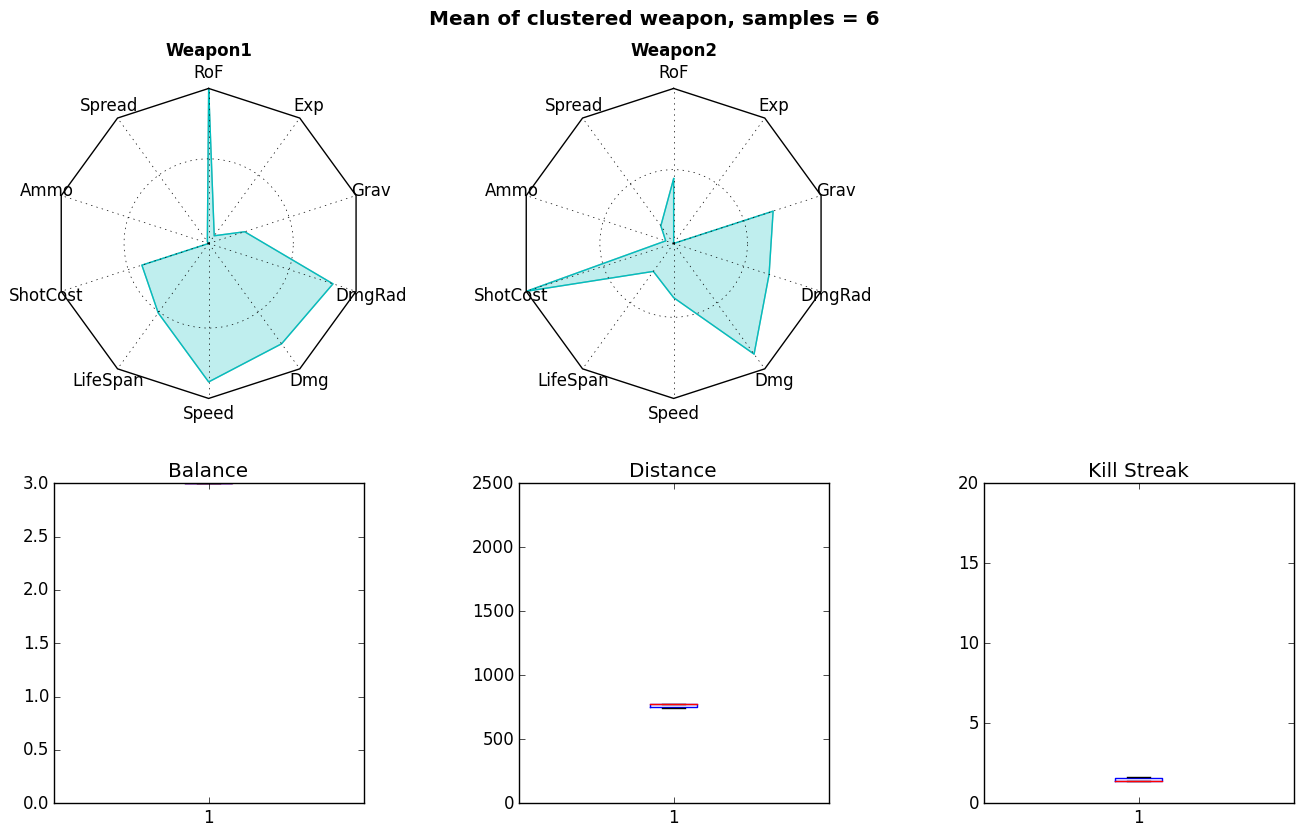
\includegraphics[width=1.0\textwidth]{rad_dist_kill_3}
\caption{\emph{radar chart} della 3°  arma generata con GA multiobiettivo (bilanciamento, distanza media e \emph{Kill Streak})}
\label{fig:rad_dist_kill_3}
\end{figure}

\section{Massimizzazione \emph{Hit time} e \emph{Kill Streak}}
\label{sec:delta_kill}

In questo esperimento andiamo a massimizzare lo \emph{Hit Time} della prima arma e la \emph{Kill Streak} della seconda.
Abbiamo condotto 10 prove di questo esperimento e abbiamo raccolto i risultati relativi alla fitness degli individui generati e le popolazioni finali ottenute nelle prove.
Ora andremo a descrivere le prestazioni dell'algoritmo dal punto di vista delle tre funzioni da massimizzare, cioè bilanciamento, \emph{Hit Time} della prima arma e \emph{Kill Streak} della seconda.
Quindi andiamo ad analizzare i risultati ottenuti usano un algoritmo di clustering sugli individui ottenuti dalle 10 prove effettuate, in modo tale da analizzarne le caratteristiche emergenti per ogni obiettivo.
Successivamente mostreremo tre esempi significativi, che massimizzano rispettivamente uno dei tre obiettivi di questo esperimento.
Infine analizzeremo l'errore con un validazione compiuta con delle valutazioni più precise dei risultati attraverso delle simulazioni con \emph{goal score} pari a 40.

\subsection{Analisi delle prestazioni}

Dopo aver effettuato 10 prove dell'esperimento abbiamo raccolto i dati relativi alla fitness delle popolazioni finali ottenute dalle prove effettuate.
Nella figura \ref{fig:pareto_dist_kill} mostriamo tre grafici: nel primo in alto a sinistra mostriamo i dati delle fitness relativi al confronto tra \emph{Hit Time} della prima arma e bilanciamento, in alto a destra mostriamo i dati relativi alla \emph{Kill Streak} della seconda arma e del bilanciamento e infine nell'ultimo grafico mostriamo il confronto tra \emph{Hit Time} della prima arma e \emph{Kill Streak} della seconda. Con i punti blu indichiamo gli individui presenti nelle popolazioni finali, mentre con i punti rossi le pareto di ogni combinazione dei tre obiettivi.

Nel grafico che confronta il bilanciamento con l'\emph{Hit time}, possiamo notare che il bilanciamento rimane massimo finché l'\emph{Hit Time} è minore di 1 secondo, dopo di che le armi hanno un rapido declino rispetto al bilanciamento. Le armi con lunghi \emph{Hit Time} sono infatti difficili da equilibrare, in quanto devono riuscire a ottenere abbastanza uccisioni nel tempo imposto dalla partita, e se i colpi colpiscono con troppo ritardo, diventa molto difficile competere con armi più veloci. 
Per quanto riguarda il confronto tra \emph{Kill Streak} e bilanciamento notiamo che, come nella sezione \ref{sec:dist_kill}, le armi bilanciate riescono a ottenere \emph{Kill Streak} non maggiori di 6 uccisioni, perché nel caso questo valore diventi maggiore di 10, il bilanciamento diventa impossibile, in quanto il massimo numero di uccisioni consentite per ottenere un'arma equilibrata è di 10 uccisioni.
Infine possiamo vedere nell'ultimo grafico che la massimizzazione della \emph{Kill Streak} non è conflittuale con lo \emph{Hit Time} e viceversa: possiamo vedere che l'algoritmo è riuscito a trovare armi che riescono a ottenere \emph{Hit Time} maggiori di 8 e \emph{Kill Streak} maggiori di 15, sebbene i limiti massimi dei due obiettivi non vengono mai raggiunti da nessuna coppia di armi.
Questo è possibile perché un'arma con dei proiettili molto lenti potenzialmente non preclude che una seconda arma riesca a ottenere lunghe sequenze di uccisioni, e viceversa.

\begin{figure}[tp]
\centering
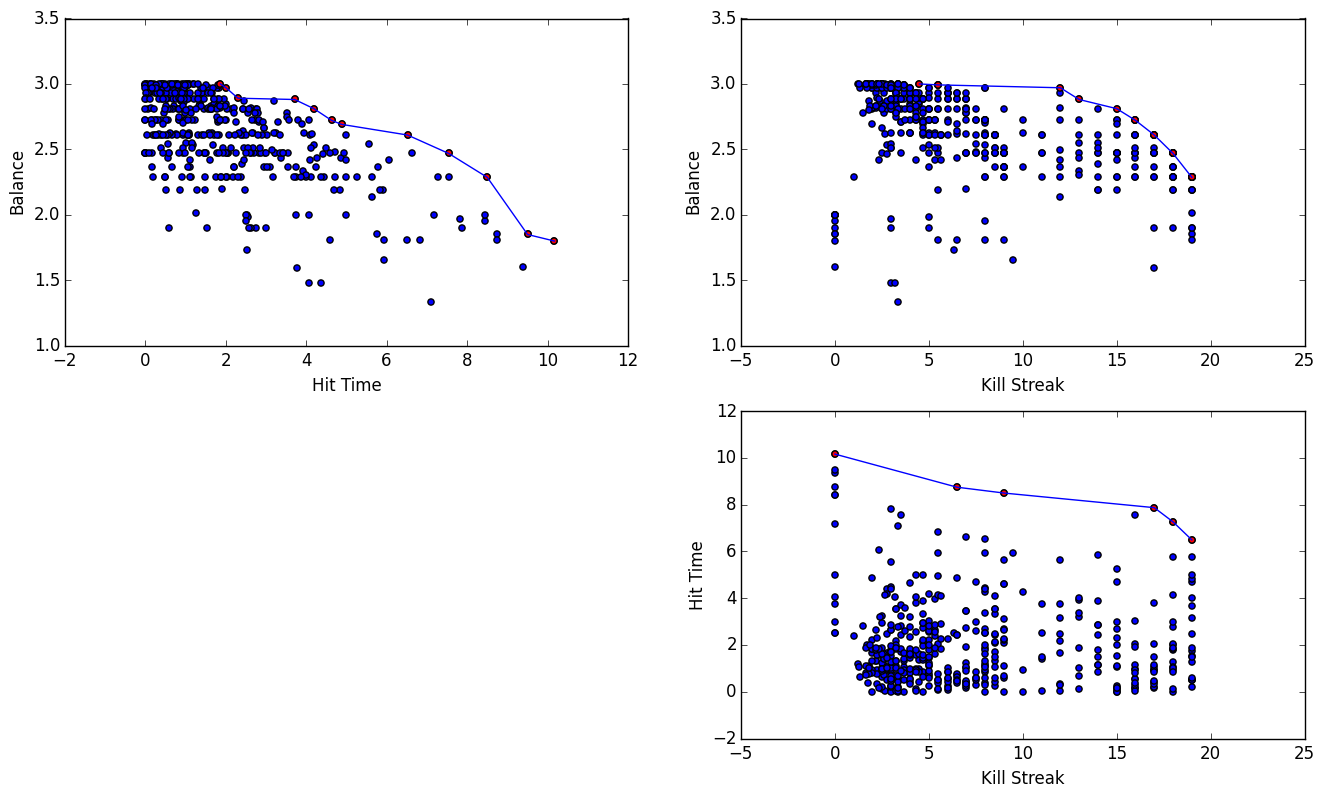
\includegraphics[width=1.0\textwidth]{pareto_delta_kill}
\caption{pareto ottenuto con il GA multiobiettivo (bilanciamento, \emph{Hit Time} e \emph{Kill Streak})}
\label{fig:pareto_delta_kill}
\end{figure}

\subsection{Analisi delle soluzioni}
\label{sec:delta_kill_sol}
Nelle 10 prove dell'esperimento di questa sezione siamo riusciti ad ottenere armi che riescono a massimizzare uno dei tre obiettivi, e sebbene nessuna coppia di armi è riuscita ad ottenere dei buoni risultati in tutti e tre gli obiettivi, abbiamo constatato che l'algoritmo è riuscito a trovare coppie armi che riescono ad ottenere prestazioni molto buone sia dal punto di vista dello \emph{Hit Time} della prima arma sia dal punto di vista della \emph{Kill Streak} per la seconda.
Per analizzare le caratteristiche delle armi trovate dall'algoritmo che riescono a massimizzare i tre obiettivi abbiamo sottoposto le popolazioni finali ottenute dalle 10 prove a un algoritmo di \emph{clustering}.
Per il clustering abbiamo utilizzato \emph{DBSCAN} con $\epsilon = 0.2$ e un numero minimo di punti per cluster pari a 5: abbiamo ottenuto 25 cluster da una popolazione finale composta da 1000 individui.

Nella figura \ref{fig:bar_delta_kill} mostriamo come si comportano in media le coppie di armi contenute nei cluster ottenuti (indicati da una lettera) per ogni parametro dell'arma. Per ogni cluster abbiamo due barre: la prima rappresenta il valore del parametro per la prima arma e la seconda rappresenta il valore del parametro per la seconda arma. In più ci sono tre grafici a barre che rappresentano rispettivamente: la media e la varianza del bilanciamento, media e varianza dello \emph{Hit Time} della prima arma e media e varianza della \emph{Kill Streak} della seconda arma.
Per la prima arma delle coppie possiamo notare che la velocità è sempre molto piccola, compresa tra i 100 $UU/s$ e 200 $UU/s$, e anche la gravità è sempre molto ridotta, con un valore in media di -20 $UU/s^2$. Infatti per ottenere armi che massimizzano lo \emph{Hit Time} l'algoritmo ha sviluppato armi che mantengono delle velocità molto basse e cercano di minimizzare il contributo dato dalla gravità, in modo tale che questa combinazione dei due parametri permetta ai proiettili di essere molto lenti e di non colpire ostacoli, come il pavimento, dovuti a una traiettoria non lineare. Purtroppo l'engine di UT3 in questo caso limite si comporta in modo poco realistico, in quanto anche con una gravità molto bassa i proiettili vengono soggetti comunque a un effetto gravitazionale abbastanza elevato. Questo ha spinto l'algoritmo a sviluppare armi con gravità sempre opposta pari a -20 $UU/{s^{2}}$: infatti la mappa usata nei nostri esperimenti è sviluppata anche in verticale, e quindi con una gravità opposta abbiamo una probabilità abbastanza alta di aumentare lo \emph{Hit Time} se l'avversario si trova a un'altezza superiore alla nostra. Inoltre la probabilità aumenta nel caso i proiettili siano esplosivi: come si può vedere il parametro \emph{explosive} della prima arma è in media maggiore di 100 UU (per esempio nei cluster B, E, F ,G) in quanto riescono a coprire un'area di danno più alta, e quindi abbiamo più possibilità di aumentare il tempo con cui colpiamo l'avversario.
Per quanto riguarda la seconda arma possiamo notare un rate di fuoco in media maggiore di 2 $proiettili/secondo$, un danno sempre maggiore di 50 e un raggio di danno in media maggiore di 50 UU. Queste armi, come nella sezione \ref{sec:dist_kill} cercano di massimizzare il danno per secondo, aumentando contemporaneamente il danno per singolo colpo e il rateo di fuoco, in modo tale da ottenere una probabilità più alta di lunghe sequenze di uccisioni.
Lo \emph{spread} di entrami le armi delle coppie ha un valore medio molto piccolo, in quanto entrambi le armi hanno bisogno di ottenere un'alta precisioni nei colpi. Infatti solo i colpi che colpiscono l'avversario influenzano le statistiche relative allo \emph{Hit Time} e alla \emph{Kill Streak}, quindi le due armi cercano di mantenere una precisione più alta possibile.
\begin{figure}[tp]
\centering
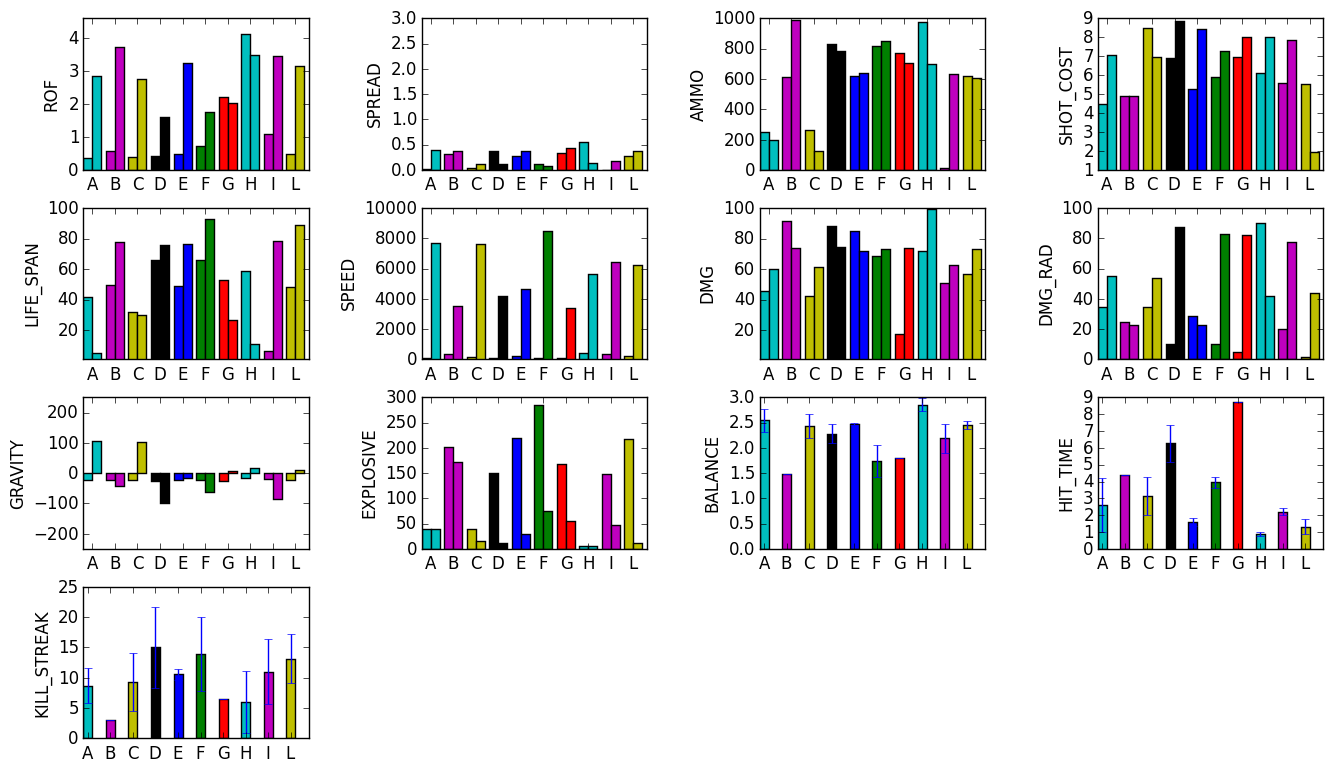
\includegraphics[width=1.2\textwidth, angle=90]{bar_delta_kill}
\caption{Grafico a barre delle armi ottenute attraverso \emph{clustering} con il GA multiobiettivo (bilanciamento, \emph{Hit Time} e \emph{Kill Streak})}
\label{fig:bar_delta_kill}
\end{figure}

\subsection{Esempi significativi}
Andremo ora a descrivere nel dettaglio tre cluster che riescono a massimizzare uno dei tre obiettivi di questo esperimento.
Nelle figure \ref{fig:rad_delta_kill_1}, \ref{fig:rad_delta_kill_2} e \ref{fig:rad_delta_kill_3} mostriamo i \emph{radar chart} dei parametri delle due armi generate ottenute come media delle armi contenute nel cluster, e inoltre mostriamo tre \emph{boxplot} dei risultati ottenute dalle armi contenute nel cluster rispetto al bilanciamento, allo \emph{Hit Time} della prima arma e alla \emph{Kill Streak} della seconda.

Il \emph{radar chart} \ref{fig:rad_delta_kill_1} mostra un coppia di armi in cui abbiamo per la prima arma uno \emph{Hit Time} in media pari a 5 secondi: la prima arma mostra una gravità molto piccola e opposta, una velocità molto bassa, e abbiamo una grande componente esplosiva dei proiettili. Questo cluster rispecchia le caratteristiche generali analizzate nella Sezione \ref{sec:delta_kill_sol}, dove abbiamo descritto come la combinazione di gravità opposta pari a -20 $UU/s^2$ e di velocità pari a 100 $UU/s$ permetta di ottenere una maggiore probabilità di colpire l'avversario con ampio ritardo.
Possiamo inoltre notare una densità di proiettili molto elevata (\emph{shotcost} pari a 9 e \emph{spread} vicino allo 0) e un rateo di fuoco contenuto che cerca di bilanciare l'alto danno causato per singolo colpo.
La seconda arma della coppia riesce a ottenere delle \emph{Kill Streak} abbastanza alte, in media comprese tra 5 e 10 uccisioni, il che dimostra come i due obiettivi, \emph{Hit Time} e \emph{Kill Streak}, possano essere ottenuti contemporaneamente in una coppia di armi.
Infine è possibile notare che il valore del bilanciamento è al di sotto di 2.5, il che mostra un'incompatibilità tra il bilanciamento e i due obiettivi secondari di questo esperimento.
\begin{figure}[tp]
\centering
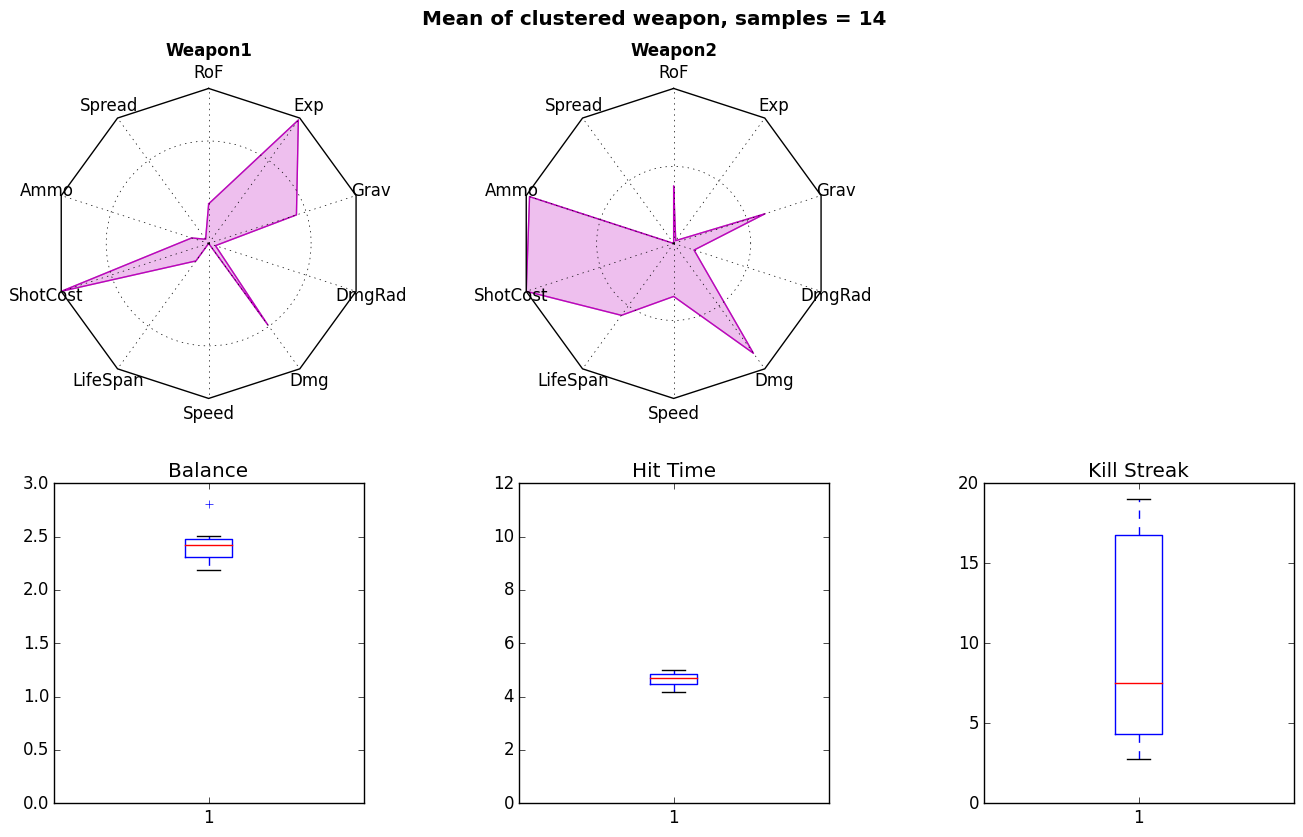
\includegraphics[width=1.0\textwidth]{rad_delta_kill_1}
\caption{\emph{radar chart} della 1°  arma generata con il GA multiobiettivo (bilanciamento, \emph{Hit Time} e \emph{Kill Streak})}
\label{fig:rad_delta_kill_1}
\end{figure}
Nel \emph{radar chart} \ref{fig:rad_delta_kill_2} la seconda arma riesce a ottenere delle \emph{Kill Streak} in media abbastanza lunghe grazie a dei proiettili che combinano velocità, danno e raggio per proiettili quasi massimi, oltre a un rateo di fuoco più alto della prima arma. La seconda arma ottimizza il danno per secondo dei proiettili, che permette di ottenere delle lunghe sequenze di uccisioni.
Anche in questo esempio l'algoritmo è riuscito a trovare coppie di armi che riuscissero a soddisfare entrambi gli obiettivi: infatti la prima arma riesce a ottenere dei \emph{Hit Time} abbastanza alti, tra i 2 e 4 secondi. 
Le caratteristiche della prima arma sono in generale molto simili a quelle analizzate nell'esempio precedente, l'unica differenza notevole è il parametro \emph{explosive}, pari a 47 UU, il che giustifica le prestazioni minori dell'arma dal punto di vista dello \emph{Hit Time}.
\begin{figure}[tp]
\centering
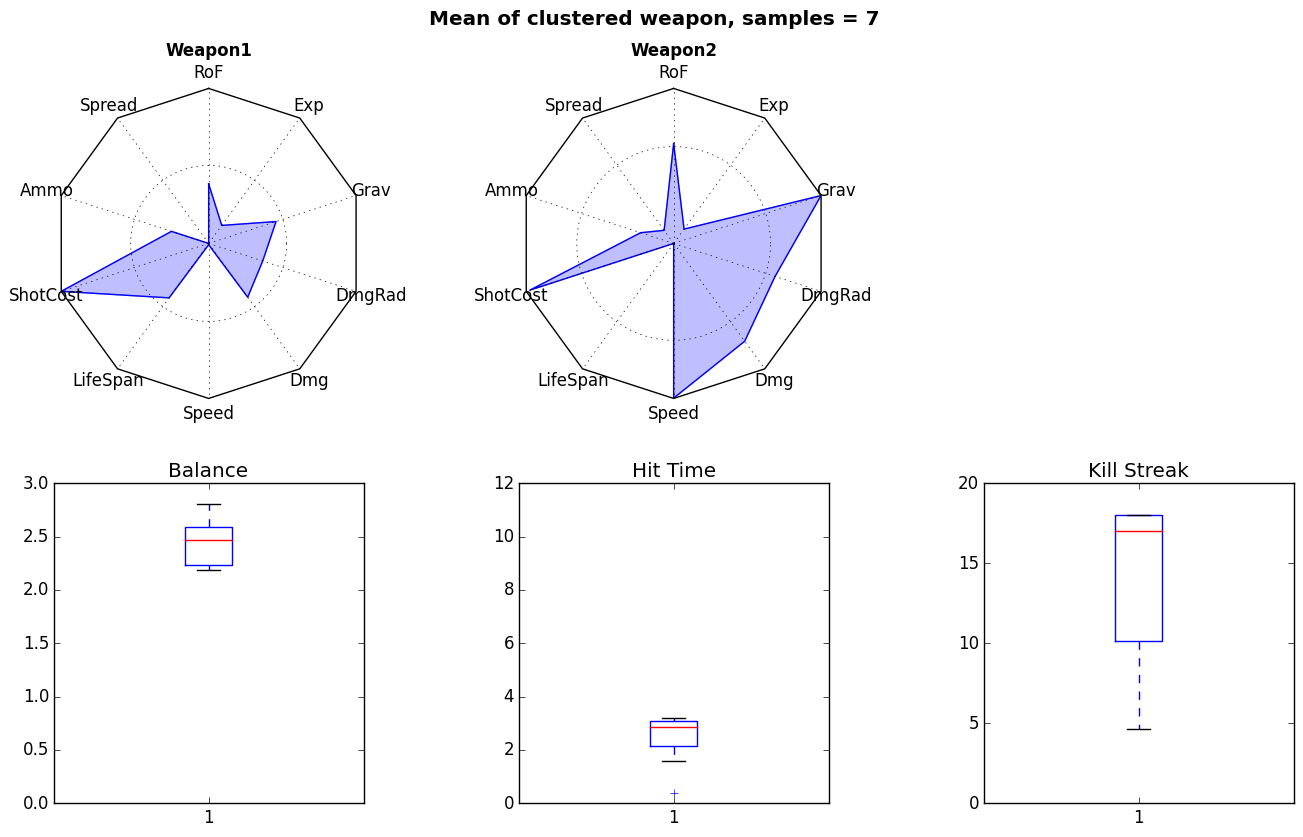
\includegraphics[width=1.0\textwidth]{rad_delta_kill_2}
\caption{\emph{radar chart} della 2° arma generata con il GA multiobiettivo (bilanciamento, \emph{Hit Time} e \emph{Kill Streak})}
\label{fig:rad_delta_kill_2}
\end{figure}
Nel terzo esempio mostriamo due armi che massimizzano il bilanciamento (vedi figura \ref{fig:rad_delta_kill_3}). Qui purtroppo dobbiamo constatare che i due obiettivi secondari non sono compatibili con il bilanciamento: infatti entrambi hanno dei risultati molto modesti sia dal punto di vista dello \emph{Hit time} e della \emph{Kill Streak}. Infatti e due armi hanno limitato proprio quelle caratteristiche che massimizzano i loro obiettivi secondari: la prima aumenta la velocità dei proiettili e diminuisce il raggio esplosivo, mentre la seconda diminuisce sia il raggio di danno dei proiettili sia il rateo di fuoco.
\begin{figure}[tp]
\centering
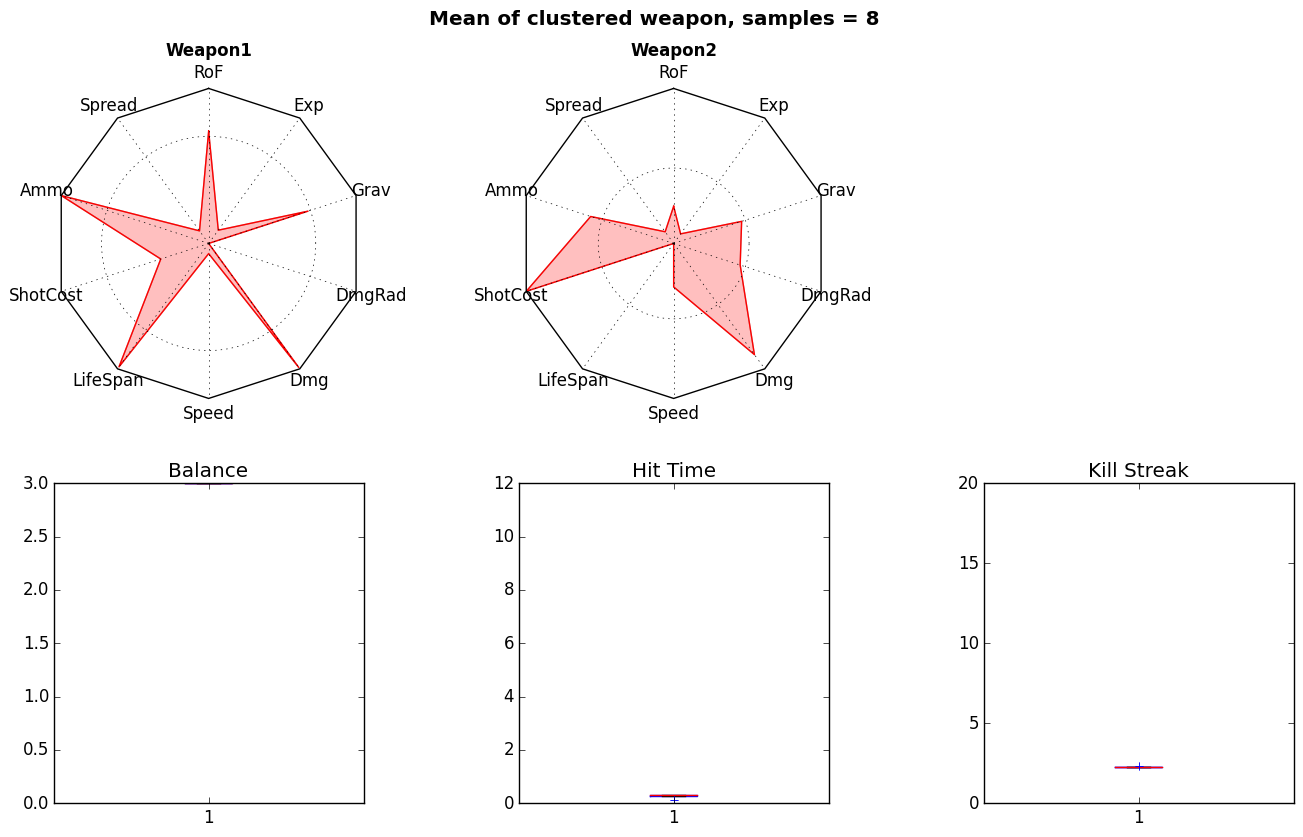
\includegraphics[width=1.0\textwidth]{rad_delta_kill_3}
\caption{\emph{radar chart} della 3° arma generata con il GA multiobiettivo (bilanciamento, \emph{Hit Time} e \emph{Kill Streak})}
\label{fig:rad_delta_kill_3}
\end{figure}

\section{Massimizzazione \emph{Hit time} e distanza media}
In questo esperimento andiamo a massimizzare lo \emph{Hit Time} della prima arma e la distanza media dei colpi della seconda arma.
Abbiamo condotto 10 prove di questo esperimento e abbiamo raccolto i risultati relativi alla fitness delle armi generate e le popolazioni finali ottenute nelle prove.
Ora andremo a descrivere le prestazioni dell'algoritmo dal punto di vista delle tre funzioni da massimizzare, cioè bilanciamento, \emph{Hit Time} della prima arma e distanza media dei colpi della seconda.
Quindi andiamo ad analizzare i risultati ottenuti usano un algoritmo di clustering sugli individui ottenuti dalle 10 prove effettuate, in modo tale da analizzarne le caratteristiche emergenti per ogni obiettivo.
Successivamente mostreremo tre esempi principali, che massimizzano rispettivamente uno dei tre obiettivi di questo esperimento.

\subsection{Analisi delle prestazioni}
\label{sec:delta_dist_prest}

Dopo aver effettuato 10 prove dell'esperimento abbiamo raccolto i dati relativi alla fitness delle popolazioni finali ottenute dalle prove effettuate.
Nella figura \ref{fig:pareto_delta_kill} mostriamo tre grafici: nel primo in alto a sinistra mostriamo i dati delle fitness relativi allo \emph{Hit Time} della prima arma e del bilanciamento, in alto a destra mostriamo i dati relativi alla distanza media dei colpi della seconda arma e del bilanciamento e infine nell'ultimo grafico mostriamo il confronto tra \emph{Hit Time} della prima arma e distanza media dei colpi della seconda. Con i punti blu indichiamo gli individui presenti nelle popolazioni finali, mentre con i punti rossi le pareto di ogni combinazione dei tre obiettivi.
Possiamo notare che i due grafici in cui compare lo \emph{Hit Time} sono molto diversi da quelli ottenuti dall'esperimento condotto nella sezione \ref{sec:delta_kill}: una popolazione (la 9°) è riuscita ad ottenere un'arma con uno \emph{Hit Time} molto più alto di quelli ottenuti fino ad ora.
Il motivo è dovuto al comportamento anomalo dell'engine UT3 che abbiamo spiegato nella sezione \ref{sec:delta_kill}: quando la velocità e la gravità dei proiettili sono molto bassi il proiettile viene comunque soggetto a una forza di gravità costante qualunque sia il valore della gravità. Però, nel caso la gravità sia esattamente zero, i proiettili non vengono più soggetti a forze di gravità, e quindi i proiettili rimangono sospesi. La popolazione presa in esame è riuscita a trovare questa particolare arma, che ottiene dei proiettil con \emph{Hit time} molto alti, in quanto questi rimangono in gioco nella posizione in cui vengono sparati finché il \emph{Life Span} non scade.
Questo comportamento anomalo dell'engine, nel quale l'accelerazione gravitazionale dei proiettili ha un impulso nel momento in cui il valore della gravità passa da 0 a un valore maggiore o minore, è un problema che non siamo riusciti a risolvere in modo completo, e richiederebbe di riscrivere il comportamento dei proiettili in UT3. Infatti è difficile per l'algoritmo genetico trovare queste armi con gravità pari a 0 in quanto non abbiamo un comportamento lineare della gravità all'interno del gioco.
Possiamo comunque notare che queste particolari armi sono dominanti rispetto a tutte le armi ottenute con le altre popolazioni, in quanto riescono anche a essere equilibrate fino a un tempo massimo di 16 secondi. 
Per quanto riguarda invece il confronto tra distanza media dei colpi e bilanciamento possiamo vedere che la distanza ha un limite oltre il quale le armi non riescono a essere bilanciate.
Questo limite è, come nell'esperimento condotto nella sezione \ref{sec:dist_kill}, pari a 1000 UU: oltre a questa distanza le armi diventano troppo avvantaggiate in quanto, avendo un raggio di fuoco troppo elevato, non permettono all'avversario di compiere nessuna uccisione.
Infine nel confronto tra \emph{Hit Time} e distanza media dei colpi vediamo che le armi che massimizzano lo \emph{Hit Time} riescono a ottenere dei valori elevati, cioè maggiori di 10 secondi, solo nel caso in cui la seconda arma non abbia una distanza media maggiore di 1000 UU: questo perché, nel caso queste ultime abbiano un raggio maggiore, diventano dominanti, e la prima arma della coppia non riesce ad effettuare abbastanza uccisioni per ottenere dei valori di \emph{Hit Time} più grandi di qualche secondo.

\begin{figure}[tp]
\centering
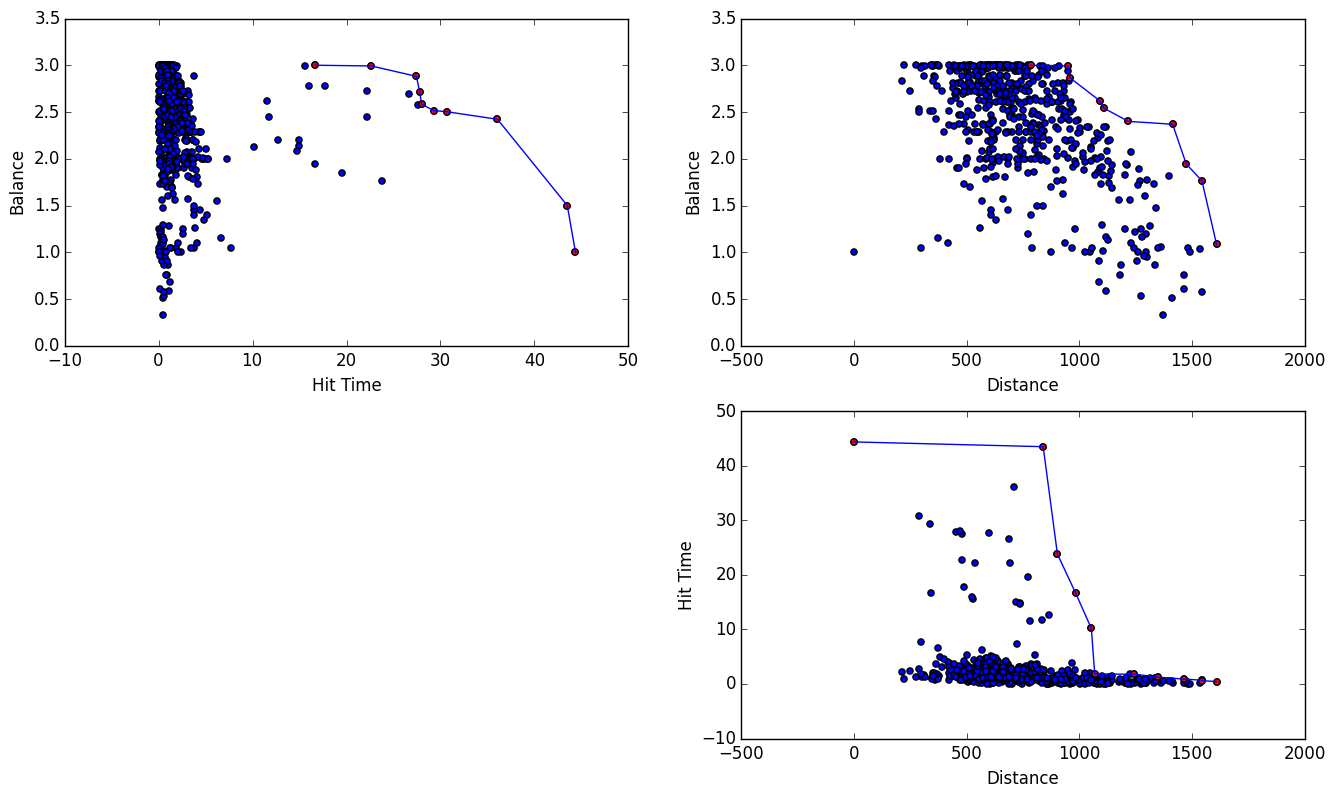
\includegraphics[width=1.0\textwidth]{pareto_delta_dist}
\caption{pareto ottenuto con il GA multiobiettivo (bilanciamento, \emph{Hit Time} e distanza media dei colpi)}
\label{fig:pareto_delta_dist}
\end{figure}

\subsection{Analisi delle soluzioni}

Nelle 10 prove dell'esperimento di questa sezione siamo riusciti ad ottenere armi che riescono a massimizzare uno dei tre obiettivi, e abbiamo potuto constatare che nel caso in cui la seconda arma delle coppie mantenga la distanza media dei colpi al di sotto di un certo valore limite, possiamo trovare delle coppie con dei buoni compromessi per tutti e tre gli obiettivi, a differenza dei due esperimenti precedenti.
Per analizzare le caratteristiche trovate dall'algoritmo che riescono a massimizzare i tre obiettivi abbiamo sottoposto le popolazioni finali ottenute dalle 10 prove a un algoritmo di \emph{clustering}.
Per il clustering abbiamo utilizzato \emph{DBSCAN} con $\epsilon = 0.2$ e un numero minimo di punti per cluster pari a 5: abbiamo ottenuto 31 cluster da una popolazione finale composta da 1000 individui.

Nella figura \ref{fig:bar_delta_dist} mostriamo come si comportano in media le coppie di armi contenute nei cluster ottenuti (indicati da una lettera) per ogni parametro dell'arma. Per ogni cluster abbiamo due barre: la prima rappresenta il valore del parametro per la prima arma e la seconda rappresenta il valore del parametro per la seconda arma. In più ci sono tre grafici a barre che rappresentano rispettivamente la media e la varianza del bilanciamento, la media e la varianza dello \emph{Hit Time} della prima arma e la media e la varianza della distanza media dei colpi della seconda arma.
Possiamo notare che le armi che massimizzano lo \emph{Hit time} (cioè le armi che compiano per prime nelle coppie) hanno sempre gravita molto vicine allo zero (nel cluster F, è esattamente zero) e velocità molto piccole, tra i 100 e i 400 $UU/s$. Questo permette di avere proiettili molto lenti e traiettorie il più possibili lineari, per quanto possibile dati i problemi dell'engine (vedi Sezione \ref{sec:delta_dist_prest}).
Invece le armi che massimizzano la distanza media (le armi che compiano per seconde nelle coppie), massimizzano la velocità, minimizzano lo \emph{spread} e in media hanno rateo di fuoco più basso rispetto alla prima arma delle coppie.
Inoltre possiamo notare che il rapporto tra gravità e velocità di queste armi è sempre molto piccolo: in questo modo la traiettoria è lineare, in quanto la gravità non riesce a essere abbastanza grande per modificarla.
Infine anche il raggio esplosivo di queste armi è sempre molto grande, in media è maggiore di 100 UU: questo permette di colpire l'avversario anche nel caso in cui non venga colpito direttamente, aumentando le statistiche relative alle distanze ottenute con l'arma.
Come possiamo notare l'algoritmo ha sviluppato alcune particolari caratteristiche per i due obiettivi secondari che possiamo ritrovare anche nei due esperimenti precedenti, sia per quanto riguarda lo \emph{Hit Time}, sia per quanto riguarda la distanza media.

\begin{figure}[tp]
\centering
\includegraphics[width=1.2\textwidth, angle=90]{bar_delta_dist}
\caption{Grafico a barre delle armi ottenute attraverso \emph{clustering} nell'esperimento di massimizzazione del bilanciamento, \emph{Hit Time} e \emph{Kill Streak}}
\label{fig:bar_delta_dist}
\end{figure}

\subsection{Esempi significativi}

Andremo ora a descrivere nel dettaglio tre cluster che riescono a massimizzare uno dei tre obiettivi di questo esperimento.
Nelle figure \ref{fig:rad_delta_dist_1}, \ref{fig:rad_delta_dist_2} e \ref{fig:rad_delta_dist_3} mostriamo i \emph{radar chart} dei parametri delle due armi generate ottenute come media delle armi contenute nel cluster, e inoltre mostriamo tre \emph{boxplot} dei risultati ottenute dalle armi contenute nel cluster rispetto al bilanciamento, allo \emph{Hit Time} della prima arma e alla distanza media dei colpi della seconda.

Nel \emph{radar chart} preso in considerazione nella figura \ref{fig:rad_delta_dist_1} mostriamo il cluster ottenuto con le armi ad alto \emph{Hit Time}: come si vede il cluster ha un massimo a 16 secondi, anche se la mediana si attesta sui 6 secondi. Questo si spiega data la particolarità dell'arma ottenuta, che permette di lasciare delle `mine' sulla mappa, e quindi il tempo con cui colpisce l'avversario è molto variabile. Inoltre l'intelligenza artificiale non comprende l'uso di una meccanica così diversa dal normale funzionamento dell'arma, il che spiega (oltre ai motivi descritti precedentemente) perché questo risultato è stato così raro da ottenere durante gli esperimenti effettuati. Questo comportamento è ottenuto con una gravità pari a zero, una velocità molto bassa (pari a 23 $UU/s$) e infine un \emph{life span} abbastanza ampio, pari a 47 secondi, che permette ai proiettili di rimanere in gioco abbastanza a lungo da poter colpire l'avversario.
Il bilanciamento di questo cluster è molto vicino al massimo teorico: 2.86. Infatti la seconda arma ha limitato il suo raggio di fuoco a 544 UU, dovuto a un valore della gravità pari a -100 $UU/s^2$, che modifica la traiettoria dei colpi e impedisce di colpire avversari troppo lontani. Questo ha permesso all'algoritmo di trovare trovare un buon compromesso tra i tre obiettivi di questo esperimento.
\begin{figure}[tp]
\centering
\includegraphics[width=1.0\textwidth]{rad_delta_dist_1}
\caption{\emph{radar chart} della 1° esempio di arma generata nell'esperimento di massimizzazione del bilanciamento, \emph{Hit Time} e \emph{Kill Streak}}
\label{fig:rad_delta_dist_1}
\end{figure}

Nel secondo esempio abbiamo la seconda arma che è riuscita a ottenere una distanza media particolarmente alta, in media pari a 1376 UU (vedi figura \ref{fig:rad_delta_dist_2}). Qui possiamo notare le caratteristiche che rendono la seconda arma molto simile a un fucile da cecchino: un danno pari al limite massimo, una velocità molto elevata, uno \emph{spread} minimo e una gravità vicina allo 0, che permettono un'alta precisione dei colpi e un raggio di fuoco elevato, in quanto i proiettili hanno una traiettoria precisa e lineare. Inoltre il rateo di fuoco è molto più contenuto in confronto alla prima arma, il che va a limitare la potenza di quest'arma.
Il bilanciamento ha un valore molto piccolo, pari a 1, il che significa che la prima arma non riesce ad ottenere nessuna uccisione, in quanto la seconda arma,  come abbiamo detto nell'analisi delle prestazioni, diventa dominante nel caso in cui la distanza media dei suoi colpi superi i 1000 UU.
\begin{figure}[tp]
\centering
\includegraphics[width=1.0\textwidth]{rad_delta_dist_2}
\caption{\emph{radar chart} della 2° esempio arma generata nell'esperimento di massimizzazione del bilanciamento, \emph{Hit Time} e \emph{Kill Streak}}
\label{fig:rad_delta_dist_2}
\end{figure}

Nel terzo esempio, prendiamo una coppia di armi perfettamente bilanciate (vedi figura \ref{fig:rad_delta_dist_3}). Qui mostriamo come la seconda arma limita il suo range di fuoco con una gravità più alta e una velocità minore rispetto al secondo esempio, oltre a limitare fortemente il danno. La prima arma d'altra parte cerca di limitare il raggio esplosivo dei proiettili (causando meno potenziali suicidi per il bot che la possiede) e riesce comunque a ottenere dei buoni risultati rispetto allo \emph{Hit Time}, nonostante un effetto gravitazione non nullo porti ad avere tempi minori rispetto all'arma analizzata nel primo esempio (vedi figura \ref{fig:rad_delta_dist_1}). 
L'algoritmo è stato capace quindi di ottenere due armi bilanciate che riescono a ottenere rispettivamente uno \emph{Hit Time} in media pari a 1 secondo e una distanza media pari a 665 UU: quindi possiamo affermare che questi tre obiettivi riescono a ottenere delle buone prestazioni contemporaneamente per un coppia di armi, a meno che la distanza media della seconda arma non superi il limite di 1000 UU.

\begin{figure}[tp]
\centering
\includegraphics[width=1.0\textwidth]{rad_delta_dist_3}
\caption{\emph{radar chart} della 3° esempio di arma generata nell'esperimento di massimizzazione del bilanciamento, \emph{Hit Time} e \emph{Kill Streak}}
\label{fig:rad_delta_dist_3}
\end{figure}

\section{Validazione}
Nella Sezione \ref{sec:goal_score} abbiamo evidenziato come le simulazioni effettuate in UT3 abbiano un errore di valutazione del bilanciamento nel caso che il \emph{goal score} sia 20.
Per validare i risultati ottenuti nei tre esperimenti, abbiamo rivalutato il bilanciamento delle popolazioni finali ottenute per i tre esperimenti con un \emph{goal score} più ampio, pari a 40, il che ci permette di avere una stima più precisa del vero valore del bilanciamento delle armi generate.
Quindi abbiamo cambiato la configurazione delle simulazioni: il limite delle uccisioni totali per partita è stato cambiato con 40, e il tempo limite delle partite è stato impostato a 2400 secondi.

\subsection{Validazione primo esperimento}
\label{sec:val_primo}

L'errore assoluto medio sul bilanciamento, calcolato come differenza tra la valutazione effettuata con \emph{goal score} pari a 40 e \emph{goal score} pari a 20, è di -0.12, con una deviazione standard di 0.31.
L'errore medio di questo esperimento è molto più grande rispetto agli esperimenti condotti nel Capitolo 4 e 5. 
Il motivo è che l'errore di valutazione diventa maggiore nel caso le armi abbiano un bilanciamento in media più basso, in quanto i tre contributi del bilanciamento, entropia, $f_g$ e $f_s$ possono diventare molto più variabili.
Infatti nei capitoli precedenti abbiamo sempre avuto delle fitness medie per il bilanciamento vicine al limite massimo teorico, il che comportava un errore dovuto a una valutazione sbagliata del solo contributo dovuto all'entropia, in quanto, a meno di casi specifici, le valutazioni relative a $f_s$ e $f_g$ erano sempre poco soggette ad errore.
Nel caso in cui però le armi non abbiano una valutazione sul bilanciamento sufficientemente alta, l'errore può essere dovuto a una combinazione di errore di tutti e tre i contributi, il che spiega l'errore in media più alto di questo esperimento.
Infatti la valutazione media del bilanciamento delle 10 prove di questo esperimento è di 2.5, una valutazione molto più bassa dovuta ai vincoli aggiunti, che come abbiamo detto, sono conflittuali rispetto al bilanciamento, e quindi portano una fitness relativa al bilanciamento più bassa.
Per quanto riguarda la varianza, questa è dovuta nuovamente alle valutazioni `diffettose' di cui abbiamo parlato nella Sezione \ref{sec:error_single_obj}.
La figura \ref{fig:error_dist_kill} mostra per ogni popolazione finale ottenuta nelle 10 prove effettuate la media e la varianza dell'errore. Come è possibile vedere, numerose popolazioni hanno ottenuto degli errori in media maggiori rispetto agli esperimenti precedenti, mentre la varianza rimane abbastanza simile come nelle validazioni effettuate nei capitoli 4 e 5. 
L'errore è in media molto spesso negativo, il che comporta che la valutazione effettuata con \emph{goal score} pari a 20 è in generale ottimistica rispetto a una valutazione più precisa effettuata con \emph{goal score} pari a 40.

\begin{figure}[tp]
\centering
\includegraphics[width=1.0\textwidth]{error_dist_kill}
\caption{errore ottenuto con la rivalutazione della popolazione finale per l'esperimento di massimizzazione del bilanciamento, distanza media dei colpi e \emph{Kill Streak}}
\label{fig:error_dist_kill}
\end{figure}

\subsection{Validazione secondo esperimento}
\label{sec:val_secondo}

L'errore assoluto medio sul bilanciamento per l'esperimento di massimizzazione dello \emph{Hit Time} per la prima arma e della \emph{Kill Streak} per la seconda, calcolato come differenza tra la valutazione effettuata con \emph{goal score} pari a 40 e \emph{goal score} pari a 20, è di -0.25, con una deviazione standard di 0.35.
Come per il primo esperimento, la media dell'errore è più alta degli esperimenti condotti nei capitoli 4 e 5. Il motivo è il medesimo: la media della fitness relativa al bilanciamento delle 10 popolazioni ottenute dalle prove dell'esperimento è pari a 2.5.
Questa media è molto più piccola rispetto al limite massimo teorico, ed è giustificata dalla ricerca di armi che soddisfino anche gli obiettivi secondari di questo esperimento, cioè lo \emph{Hit Time} e la \emph{Kill Streak}.
Purtroppo questo porta a un errore maggiore, perché la valutazione diventa più imprecisa dovuto all'errore introdotto da tutte e tre le funzioni che contribuiscono a valutare il bilanciamento, cioè entropia, $f_g$ e $f_s$.
La varianza invece è dovuta alle simulazioni errate citate nella Sezione \ref{sec:error_single_obj}.
La figura \ref{fig:error_delta_kill} mostra la media e la varianza dell'errore, calcolato come differenza tra la valutazione effettuata con \emph{goal score} pari a 40 e \emph{goal score} pari a 20, delle singole popolazioni ottenute nelle 10 prove effettuate: possiamo notare come l'errore in media sia sempre negativo, il che significa che con un \emph{goal score} pari a 20 abbiamo avuto una valutazione ottimistica rispetto alla valutazione più precisa ottenuta con \emph{goal score} pari a 40; inoltre la varianza rimane costante per tutte le popolazioni, il che mostra come non sia una popolazione particolare a incrementare la varianza.

\begin{figure}[tp]
\centering
\includegraphics[width=1.0\textwidth]{error_delta_kill}
\caption{errore ottenuto con la rivalutazione della popolazione finale per l'esperimento di massimizzazione del bilanciamento, \emph{Hit Time} e \emph{Kill Streak}}
\label{fig:error_delta_kill}
\end{figure}

\subsection{Validazione terzo esperimento}

L'errore assoluto medio sul bilanciamento per l'esperimento di massimizzazione dello \emph{Hit Time} per la prima arma e della distanza media dei colpi per la seconda, calcolato come differenza tra la valutazione effettuata con \emph{goal score} pari a 40 e \emph{goal score} pari a 20, è di -0.096, con una deviazione standard di 0.50.
Abbiamo un incremento delle media rispetto alle validazioni effettuate nei capitoli 4 e 5, e in questo caso anche un incremento della varianza. Questo è dovuto alle prestazioni ottenute in questo esperimento dal punto di vista del bilanciamento.
Infatti la media della fitness relativa al bilanciamento delle 10 popolazioni finali ottenute nelle prove dell'esperimento effettuate è $2.3$. 
Questa media è giustificata dalla ricerca di armi che soddisfino anche gli obiettivi secondari di questo esperimento, cioè l'\emph{Hit Time} e la distanza media dei colpi, il che comporta un bilanciamento medio delle armi più basso.
Purtroppo questo porta a un errore maggiore, perché la valutazione diventa più imprecisa dovuto all'errore introdotto da tutte e tre le funzioni che contribuiscono a valutare il bilanciamento, cioè entropia, $f_g$ e $f_s$.
Anche la varianza pare essere aumentata rispetto alle validazioni precedenti: anche questo è dovuto alla fitness media del bilanciamento, in quanto una valutazione così bassa incrementa le probabilità di aver ottenuto un errore nelle valutazioni con \emph{goal score} pari a 20, che deve essere aggiunto all'errore introdotto dalle simulazioni errate citate nella Sezione \ref{sec:error_single_obj} 
La figura \ref{fig:error_delta_kill} mostra la media e la varianza dell'errore, calcolato come differenza tra la valutazione effettuata con \emph{goal score} pari a 40 e \emph{goal score} pari a 20, delle singole popolazioni ottenute nelle 10 prove effettuate: possiamo notare come l'errore in media sia sempre negativo, il che significa che con un \emph{goal score} pari a 20 abbiamo avuto una valutazione molto spesso ottimistica rispetto alla valutazione più precisa ottenuta con \emph{goal score} pari a 40; inoltre possiamo notare come la varianza sia costante per tutte le popolazioni.

\begin{figure}[tp]
\centering
\includegraphics[width=1.0\textwidth]{error_delta_dist}
\caption{errore ottenuto con la rivalutazione della popolazione finale per l'esperimento di massimizzazione del bilanciamento, \emph{Hit Time} e distanza media dei colpi}
\label{fig:error_delta_dist}
\end{figure}

\section{Sommario}
In questo capitolo abbiamo descritto gli esperimenti compiuti per generare armi bilanciate con vincoli aggiuntivi.
Nella Sezione 6.1 abbiamo descritto le armi generate con gli obiettivi aggiuntivi riguardanti la distanza media dei colpi per la prima arma e la \emph{kill streak} per la seconda.
Nella Sezione 6.2 abbiamo riportato i risultatati ottenuti con gli obiettivi aggiuntivi riguardanti lo \emph{Hit Time} per la prima arma e la \emph{kill streak} per la seconda.
Nella Sezione 6.3 parliamo dei risultati ottenuti con gli obiettivi aggiuntivi riguardanti lo \emph{Hit Time} per la prima arma e la distanza media dei colpi per la seconda.
Infine nella Sezione 6.4 descriviamo i risultati ottenuti con la validazione dei tre esperimenti effettuati con una validazione del bilanciamento con \emph{goal score} pari a 40.


 
\chapter{Conclusioni e sviluppi futuri}

In questo lavoro abbiamo affrontato il problema di generare armi bilanciate per un videogioco sparatutto in prima persona.
Per risolvere questo problema abbiamo sviluppato uno strumento per generare automaticamente armi per il gioco \emph{Unreal Tournament III}.

\section{Conclusioni}

Per valutare le due armi generate eseguiamo una simulazione tra due giocatori controllati dall'intelligenza artificiale, con un determinato numero di uccisioni per partita e un tempo limite. Quando la simulazione termina raccogliamo i risultati e attraverso la funzione di fitness ne valutiamo le prestazioni.
Abbiamo condotto alcuni test per decidere come impostare la velocità e il numero di uccisioni per partita della simulazione, in modo tale che avessimo un compromesso accettabile tra tempo richiesto da una simulazione e l'errore nei dati raccolti.
Successivamente abbiamo condotto tre diversi tipi di esperimenti.
Nel primo abbiamo generato delle armi bilanciate con un algoritmo genetico a singolo obiettivo. La funzione obiettivo si compone di tre funzioni: la prima valuta il bilanciamento relativo alle uccisioni ottenute, la seconda l'efficacia e infine la terza l'usabilità.
I risultati mostrano che l'algoritmo riesce a ottenere una popolazione con fitness media vicina al limite massimo teorico e dimostra inoltre un notevole potenziale creativo, come si può vedere dal numero notevole di armi differenti generate. Infatti analizzando i dati è possibile trovare sia armi simili a quelle classiche che è possibile trovare negli sparatutto in prima persona, come per esempio i fucili da cecchino, sia armi completamente originali.
Nel secondo esperimento abbiamo provato a migliorare un'arma presente nel gioco, il \emph{Flak}, per renderla equilibrata rispetto un'altra arma, il \emph{Rocket Launcher}, entrambi armi presenti in Unreal Tournament III.
L'algoritmo è stato capace di trovare due soluzioni molto simili all'arma obiettivo e bilanciate rispetto \emph{Rocket Launcher}, il che dimostra come sia possibile utilizzare questo lavoro per automatizzare il bilanciamento di due armi create \emph{ad hoc} dai game designer. In particolare la prima soluzione aumenta il rateo di fuoco dell'arma, mentre nella seconda soluzione vengono aumentati il numero di munizioni e il raggio esplosivo dei proiettili.
Infine nel terzo esperimento abbiamo provato a estendere la generazione aggiungendo degli obiettivi secondari, cioè la distanza media dei colpi, la sequenza media di uccisioni senza interruzioni (\emph{Kill Streak}) e il tempo medio impiegato per colpire l'avversario (\emph{Hit Time}).
I risultati ottenuti massimizzando la distanza media dei colpi per la prima arma e la \emph{Kill Streak} per la seconda mostrano che questi due obiettivi sono inversamente proporzionali: se la distanza media dei colpi diventa troppo alta, la seconda arma non riesce a colpire l'avversario, mentre nel caso la \emph{Kill Streak} della seconda arma sia vicina al massimo teorico, la seconda arma riesce ad effettuare la maggior parte delle uccisioni, rendendo la partita squilibrata. Per massimizzare la distanza l'algoritmo ha generato armi con una gravità molto bassa, un'alta velocità e un \emph{spread} quasi nullo; invece per massimizzare la \emph{Kill Streak} l'algoritmo ha prodotto armi con un rateo di fuoco molto alto, un danno e un raggio di danno per proiettile molto elevati. Infine i risultati mostrano che le due armi per risultare equilibrate devono limitare i loro obiettivi secondari, cioè mostrano dei risultati modesti sia dal punto di vista della distanza media ottenuta dalla prima arma sia dal punto di vista della \emph{Kill Streak} della seconda arma.
I risultati ottenuti massimizzando lo \emph{Hit Time} per la prima arma e la \emph{Kill Streak} per la seconda mostrano che questi due obiettivi non sono per sé conflittuali, ma l'algoritmo non è riuscito a generare armi equilibrate che riuscissero a soddisfare in parte gli obiettivi secondari, cioè abbiamo una incompatibilità tra il bilanciamento e la combinazione di questi due obiettivi.
Per massimizzare lo \emph{Hit Time} l'algoritmo ha generato armi con una gravità molto bassa e opposta, una velocità ridotta e un raggio esplosivo dell'arma abbastanza alto. Per quanto riguarda la \emph{Kill Streak} valgono le medesime considerazioni fatte nell'esperimento precedente.
I risultati ottenuti massimizzando \emph{Hit Time} e \emph{Distance} mostrano che le armi a lungo raggio diventano dominanti rispetto a qualsiasi tipo di arma, mentre nel caso la seconda arma limiti parzialmente il suo raggio di fuoco, l'algoritmo è capace di creare coppie di armi equilibrate con \emph{Hit Time} e distanza media mediamente alti. Infatti in questo esperimento abbiamo trovato coppie armi che sono riuscite a ottenere buone prestazioni in tutti e tre gli obiettivi contemporaneamente, a differenza dei due esperimenti precedenti.

\section{Validazione bilanciamento}

Per valutare l'attendibilità della valutazione della fitness utilizzata per calcolare il bilanciamento delle armi generate, abbiamo condotto dei test con delle persone fisiche, che hanno provato una sessione di gioco con delle armi generate dall'algoritmo.
Abbiamo scelto due coppie di armi generate con l'esperimento effettuato nel capitolo 4, coppie che hanno ottenuto due diverse valutazioni della fitness, una con una valutazione vicina al limite massimo teorico e una con una valutazione minore.
Queste armi sono state scelte in quanto abbiamo voluto vedere se effettivamente la valutazione delle persone cambiava a seconda della valutazione più alta o più bassa ottenuta nella fitness.
La seconda coppia che ha ottenuto una fitness più bassa è stata scelta in quanto ha ottenuto una valutazione minore solo nel contributo relativo all'entropia, mentre per quanto riguarda gli altri due contributi relativi a suicidi e numero di uccisioni (vedi capitolo 4, Sezione 4.1) abbiamo una valutazione massima.
In questo modo ci siamo assicurati che anche la seconda coppia di armi fosse funzionale e potesse essere utilizzata dagli utenti e che l'unica differenza fosse nella valutazione dell'equilibrio delle due armi.
La prova è stata effettuata con la seguente configurazione: al giocatore venivano assegnate le due armi da testare, una di colore blu e una di colore rosso, e venivano fatti giocare contro l'intelligenza artificiale, a cui veniva assegnata dinamicamente l'arma della coppia non utilizzata in quel momento dal giocatore, affinché potessimo valutare il bilanciamento delle due armi. 
Nella figure \ref{fig:weap_test_1} e \ref{fig:weap_test_2} mostriamo i \emph{radar chart} dei parametri delle due coppie di armi utilizzate per la validazione, dove abbiamo chiamato \emph{arma blu} la prima arma fornita agli utenti e \emph{arma rossa} la seconda arma fornita.
\begin{figure}[htp]
\centering
\includegraphics[width=1.0\textwidth]{weap_test_1}
\caption{\emph{radar chart} della prima coppia di armi testata nella validazione con persone fisiche}
\label{fig:weap_test_1}
\end{figure}

\begin{figure}[htp]
\centering
\includegraphics[width=1.0\textwidth]{weap_test_2}
\caption{\emph{radar chart} della seconda coppia di armi testata nella validazione con persone fisiche}
\label{fig:weap_test_2}
\end{figure}
Le partite sono state eseguite con un limite di uccisioni totali (\emph{goal score}) pari a 10 e una durata massima di 10 minuti.
Dopo ogni partita abbiamo chiesto ai partecipanti di compilare un questionario, con domande relative alla loro esperienza di gioco.
In particolare abbiamo chiesto quale arma hanno preferito delle due utilizzate e di valutare con tre opzioni (poco, medio e alto) il divertimento e con altre tre opzioni (svantaggio, equilibrio, vantaggio) il bilanciamento della coppia di armi provate.
Abbiamo raccolto un totale di 35 prove, di cui 17 sono state eseguite con la coppia di armi con fitness massima e 18 con la coppia di armi con fitness minore.
Nelle figure \ref{fig:val_2} e \ref{fig:val_2} mostriamo i risultati ottenuti nelle prove effettuate con le due coppie: mostriamo cinque grafici che riassumono le risposte ottenute dai questionari, dove il primo grafico mostra per le due armi (blu e rossa) la percentuale delle preferenze, mentre nei grafici seguenti mostriamo le percentuali delle risposte relative al divertimento e al bilanciamento delle due armi della coppia, rispettivamente la prima di colore blu e la seconda di colore rosso.
La figura \ref{fig:val_2} e \ref{fig:val_1} mostrano i risultati ottenuti con la prima e la seconda coppia di armi selezionate.
\begin{figure}[htp]
\centering
\includegraphics[width=1.0\textwidth]{validation_2}
\caption{percentuali delle risposte ottenute dai gli utenti rispetto i test effettuati con la prima coppia di armi}
\label{fig:val_2}
\end{figure}
\begin{figure}[htp]
\centering
\includegraphics[width=1.0\textwidth]{validation_1}
\caption{percentuali delle risposte ottenute dai gli utenti rispetto i test effettuati con la seconda coppia di armi}
\label{fig:val_1}
\end{figure}
Dai grafici possiamo notare che gli utenti hanno considerato molto più bilanciata la seconda coppia di armi rispetto alla prima.
Se analizziamo i risultati della prima coppia di armi (vedi figura \ref{fig:val_2}) notiamo come l'arma blu sia stata preferita dal 70\% delle persone, e se ci concentriamo sul bilanciamento notiamo come per l'arma blu abbiamo un 40\% di persone che hanno considerato l'arma bilanciata e la medesima quantità di persone ha considerato l'arma avvantaggiata; al contrario il 41\% di persone ha considerato l'arma rossa bilanciata e un altrettanto numero di persone ha considerato invece l'arma svantaggiata rispetto all'arma blu.
Invece nei grafici relativi alla seconda coppia di armi (vedi figura \ref{fig:val_1}) per quanto riguarda il bilanciamento il 60\% degli utenti ha considerato entrambi le armi bilanciate, mentre per quanto riguarda la preferenza tra le due armi abbiamo una differenza minima tra prima e seconda arma. 
Dai dati possiamo concludere che gli utenti hanno considerato la prima coppia di armi più sbilanciata rispetto alla seconda coppia: quindi i test hanno dato dei risultati opposti a quelli previsti dalla simulazione, che aveva valutato più sbilanciate la seconda coppia e più bilanciata la prima.
Il motivo è che nella prima coppia, le armi sono molto particolari (vedi figura \ref{fig:weap_test_1}): queste armi sono molto diverse nel loro utilizzo, in quanto l'arma blu è utilizzabile per le lunghe distanze, mentre la seconda arma è più efficace a corto raggio, avendo una combinazione di gravità e velocità che determina delle traiettorie paraboliche dei proiettili molto ravvicinate.
Inoltre la seconda arma necessita una grande precisione dei colpi, e nel caso l'avversario venga colpito, questo viene immediatamente ucciso dal colpo, a differenza della prima, che ha bisogno di più colpi per uccidere l'avversario.
Gli utenti si sono trovati in difficoltà nell'utilizzare la seconda arma, date la sua peculiare modalità di fuoco, molto diversa dalle normali modalità di fuoco delle armi.
Hanno quindi preferito utilizzare un'arma più classica, cioè l'arma blu, che assomiglia a un fucile in quanto può colpire sulle medie e lunghe distanze.
Nel caso invece della seconda coppia di armi, queste hanno una modalità d'uso più classica e più facilmente comprensibile, il che ha comportato un giudizio più favorevole rispetto a questa coppia di armi.


\section{Sviluppi Futuri}

Uno dei sviluppi futuri di questo lavoro sarà generare contemporaneamente le mappe e le armi per un videogioco sparatutto in prima persona. Infatti nei nostri esperimenti abbiamo supposto che la mappa scelta per le simulazioni fosse ininfluente rispetto al bilanciamento della partita. In verità questa è una semplificazione che abbiamo adottato per poterci concentrare sulla generazione delle armi, ma sarebbe interessante estendere il lavoro svolto con un algoritmo coevolutivo che generi contemporaneamente le armi e le mappe per il gioco, utilizzando le tecniche sviluppate per generare le mappe che si possono trovare in letteratura (come nel lavoro di Cardamone et al. \cite{fpsmaps:article}).
Un altro sviluppo possibile potrebbe essere estendere le funzionalità delle armi presenti nel gioco UT3, aggiungendo effetti procedurali come nel lavoro di Erin J. Hastingsa et al. \cite{gar:article}, sempre cercando di generare armi equilibrate. Questo comporterebbe modificare l'intelligenza artificiale del gioco per poter simulare correttamente le partite. Per esempio si potrebbero modificare sia il comportamento dei proiettili, per esempio utilizzando \emph{cgNEAT}, sia aggiungendo effetti aggiuntivi ai danni possibili, come avvelenamento, guarigione, elettrici ecc.

\cleardoublepage
\phantomsection
\addcontentsline{toc}{chapter}{\bibname}
\printbibliography

\end{document}